
\documentclass[leqno]{memoir}
\usepackage{graphicx}
\usepackage{pdfpages}

\usepackage{zref-abspage}
\usepackage{atveryend}

\chapterstyle{article}

\title{Matthew's Songbook}

\makeatletter
% Because of starred chapters we need an extra chapter counter
% for identifying a chapter. \thechapter is not unique in general.
\newcounter{abschap}
\renewcommand*{\theabschap}[1]{abschap.\the\value{abschap}.#1}

\renewcommand*{\clearforchapter}{%
  \EndChapter
  \stepcounter{abschap}%
  \zref@refused{\theabschap{beg}}%
  \zref@refused{\theabschap{end}}%
  \def\ClearChapter{\cleartoverso}%
  \zref@ifrefundefined{\theabschap{beg}}{%
  }{%
    \zref@ifrefundefined{\theabschap{end}}{%
    }{%
      \ifnum\numexpr
        \zref@extract{\theabschap{end}}{abspage}%
        -\zref@extract{\theabschap{beg}}{abspage}%
      = 1 %
        \let\ClearChapter\@empty
      \fi
    }%
  }%
  \ClearChapter
  \zref@wrapper@immediate{%
    \zref@labelbyprops{\theabschap{beg}}{abspage}%
  }%
}
\newcommand*{\EndChapter}{%
  % flush floats
  \clearpage
  % Set an anchor after the last page with contents of the current
  % chapter.
  \zref@wrapper@immediate{%
    \@ifundefined{\theabschap{end}}{%
      \zref@labelbyprops{\theabschap{end}}{abspage}%
      \global\expandafter\let\csname\theabschap{end}\endcsname\@empty
    }{}%
  }%
}
\AfterLastShipout{\EndChapter}
\newcommand*{\org@part}{}
\let\org@part\part
\renewcommand*{\part}{%
  \EndChapter
  \org@part
}
\makeatother


\begin{document}

\pagestyle{headings}
\setcounter{page}{1}
\pagenumbering{roman}

\tableofcontents



\chapter{NORTHWEST PASSAGE - Stan Rogers}
\setcounter{page}{1}
\pagenumbering{arabic}

\begin{verbatim}
from the album "Northwest Passage"
(c) 1981 Fogarty's Cove Music Inc.

               D        A            G                  Bm
        Ah for just one time I would take the Northwest Passage
           G                D                 Em               G
        To find the hand of Franklin reaching for the Beaufort Sea
                D        A              G                Bm
        Tracing one warm line through a land so wide and savage
            G                D       A      D
        And make a Northwest Passage to the sea

Westward from the Davis Strait, 'tis there was said to lie
The sea route to the orient for which so many died
Seeking gold and glory, leaving weathered broken bones
And a long forgotten lonely cairn of stones

Three centuries thereafter I take passage over land
In the footsteps of brave Kelso where his "sea of flowers" began
Watching cities rise before me then behind me sink again
This tardiest explorer driving hard across the plains

And through the night behind the wheel, the mileage clicking west
I think upon Mackenzie, David Thompson, and the rest
Who cracked the mountain ramparts and did show a path for me
To race the roaring Fraser to the sea

How then am I so different from the first men through this way
Like them, I left a settled life, I threw it all away
To seek a Northwest Passage at the call of many men
To find there but the road back home again
\end{verbatim}
\newpage

\chapter{Famous Inside}
Capo 3rd fret works good
\begin{verbatim}
      G
I can almost hear some of you say,
       G
"You'd think he'd have more sense at his age,
    C
The crazy old man in the old tam-o-shanter's
        G
Getting carried away."

Sometimes it's almost too much to stand,
But it's not my place to take you in hand.
It used to be a man and his madness
Were as sacred as the coming of day.

It's strange how things will stick in the mind.
You'd think the years would leave them behind,
But long ago moments as a winner
Kind of push the recent memories aside.

Symptomatic, you say, of old age,
But it's something that nobody can gage.
It may be that I've sorted out the memories I can keep
And thrown the others away.

D
There's some who would say, "Just let him sit and decay",
      C                              G
But I really can't believe that it's true.
        F#7
There's bits of yourself you always have to live up to
   C                    D7
If only for a moment or two!

There's little time to spend sitting down,
When feeling good means moving around,
And I can't be blamed if I remember my name
And why it made me so proud.

There's some who would say, "Just let him sit and decay",
But I really can't believe that it's true!
There's bits of yourself you always have to live up to,
If only for a moment or two!

At my age I do as I choose,
And shouldn't need to make an excuse.
I know that you all feel a little famous inside
And I'm no different than you.
I know that you all feel a little famous inside,
And I'm no different than you.
\end{verbatim}
\newpage

\chapter{Down the Road}
\begin{verbatim}
G Em C G  
Em C G
G G/D C/E C     
Em C G

G             Em  C                 G
Sun is rising high, burning into the day,
               Em C               G
I will say goodbye, I'll be going away,
              G      G/D                 C/E C
Brush away my doubts, what tomorrow will hold,
                 Em C               G
Feeling fine for now, going down the road...


             Em  C                        G
To a city to sing, about the trees and the wind,
                   Em    C                    G
'Bout the hills in spring, and the rivers that bend,
               G    G/D                  C/E C
The rocky deep pass, and the poppies and posies,
                    Em   C                G
Running through the grass, up and down the road.


           Em C              G
Do do do dodo  do do do do do do
           Em C              G
Do do do dodo  do do do do do do 
                 G  G/D            C/E C
Do do do do do dodo do do do do do do   do 
           Em C              G
Do do do dodo  do do do do do do 


                 Em C                    G
In the dark they sit  and they holler for more,
                 Em  C                 G
White smoke in a wisp, from here to the door,
                     G    G/D                      C/E C
Their admission they paid, for the stories they're told,
               Em C                    G
Of a clear new day, hold me down on the road.


                    Em  C              G
So heavy rain at my back, lazy meadows ahead,
                  Em   C                G
In my book I keep track, of the promises said.
                  G    G/D                 C/E C
For my songs in a town, that tomorrow will hold
                 Em C                G
Feelin' fine for now, facin' down the road.


           Em C              G
Do do do dodo  do do do do do do
           Em C              G
Do do do dodo  do do do do do do 
                 G  G/D            C/E C
Do do do do do dodo do do do do do do   do 
           Em C              G
Do do do dodo  do do do do do do 


              Em  C                 G
Sun is rising high, burning into the day,
               Em C               G
I will say goodbye, I'll be going away,
                   G      G/D                 C/E C
I'll brush away my doubts, what tomorrow will hold,
                     Em C               G
I'm feeling fine for now, going down the road...
                     Em C               G
I'm feeling fine for now, going down the road...
                     Em C               G
I'm feeling fine for now, going down the road.


           Em C              G
Do do do dodo  do do do do do do
           Em C              G
Do do do dodo  do do do do do do 
                 G  G/D            C/E C
Do do do do do dodo do do do do do do   do 
           Em C              G
Do do do dodo  do do do do do do
\end{verbatim}
\newpage

\chapter{Barretts Privateers}
\begin{verbatim}
        1        *         5       1
Oh, the year was seventeen seventy-eight
      *      4      1          5     (*)
How I wish I was in Sherbrooke now
  1         5           1        *
A letter of marque came from the king
       *         *          5    4
To the scummiest vessel I'd ever seen


CHORUS:
    5         1    *     4
God damn them all, I was told,
     1          4          1       4
We'd cruise the seas for A-merican gold
     5       1     5       4     (*)
We'd fire no guns, shed no tears
          1      4        1       4
But I'm a broken man on a Halifax pier
    *       *         5     1
The last of Barrett's Priva-teers


    1     *       5         1
Oh, Elcid Barrett cried the town
      *      4      1          5    (*)
How I wish I was in Sherbrooke now
    1            5        1          *
For twenty brave men, all fishermen, who
      *        *       5          4
Would make for him the Antelope's crew

    1        *           5         1
The Antelope sloop was a sickening sight
      *      4      1          5    (*)
How I wish I was in Sherbrooke now
        1           5            1        *
She'd a list to the port and her sails in rags
        *           *                 5            4
And the cook in the scuppers with the staggers and jags

       1            *      5      1
On the King's birth-day we put to sea
      *      4      1          5    (*)
How I wish I was in Sherbrooke now
        1          5           1    *
We were ninety-one days to Mon-tego Bay
*            *      5       4
Pumping like madmen all the way



       1            *      5        1
On the ninety-sixth day we sailed a-gain
      *      4      1          4    (*)
How I wish I was in Sherbrooke now
       1            5      1       *
When a bloody great Yankee hove in sight
         *            *            5       1
With our cracked four-pounders, we made to fight


    1      *       5         1
The Yankee lay low down with gold
      *      4      1          5     (*)
How I wish I was in Sherbrooke now
        1         5       1        *
She was broad and fat and loose in stays
       *                  *        5         1
But to catch her took the Antelope two whole days

        1         *         5        1
Then at length we stood two cables a-way
      *      4      1          5     (*)
How I wish I was in Sherbrooke now
    1            5                1     *
Our cracked four-pounders made an awful din
         *       *             5        1
But with one fat ball the Yank stove us in


    1        *         5              1
The Antelope shook and pitched on her side
      *      4      1          5     (*)
How I wish I was in Sherbrooke now
1           5              1       *
Barrett was smashed like a bowl of eggs
        *          *           5       1
And the main-truck carried off both me legs


   1      *         5            1
So here I lay in my twenty-third year
      *      4      1          5     (*)
How I wish I was in Sherbrooke now
     1        5              1        *
It's been six years since we sailed a-way
      *         *       5      1
And I just made Halifax yester-day
\end{verbatim}
\newpage


\chapter{THE WOODBRIDGE DOG DISASTER}
(Written by Royston Wood as performed by Stan Rogers)
\begin{verbatim}
There was an old woman in Woodbridge, there was,
So proper and tidy and all of those things,
She would wander all day with her duster in hand.
She was one of those women who cleaned where they stand,
And while she is at it she sings, boys!
And while she is at it, she sings!

Now, there's no doubt about it, her house was a show,
With everything proper and stowed in its place,
And that's why her dustbins had a shed of their own.
Like a mirror, each one of those bins it had grown!
You could read every line in your face, boys!
You could read every line in your face!

Now, there's nothing the matter with tidiness, no,
No matter with keeping your house up to scratch,
But these bins were located one side of a yard,
Where a Doberman Pinscher was prowling on guard,
Trained to kill if you lifted the latch, boys!
Trained to kill if you lifted the latch!

Now it's all very well to protect what is yours,
And it's better not leaving temptation around,
But a job on the "dust" is rewarding enough,
And there's nothing like taking the smooth with the rough,
To be savaged by some bloody hound, boys!
To be savaged by some bloody hound!

Now, this Doberman Pinscher would play in the yard,
And a couple of old tennis balls as its game.
In his make-believe game, it's himself that he saw,
As the world's only dog with a bionic jaw,
And that's when the garbage-man came, boys!
And that's when the garbage-man came!

Now, fate took a hand on this coldest of days,
For his wife, she had made him to wear a warm coat,
And to knot up his muffler to keep out the chill,
And, for once in his life, he had bent to her will,
And the dog couldn't get at his throat, boys!
And the dog couldn't get at his throat!

Now, when the woman above was drawn to the noise,
It's down from a high chamber-window she calls,
To the dustman, engaged in a struggle for life,
In a middle-class tone you could cut with a knife,
She loudly exclaimed, "Kick his balls!" boys!
She loudly exclaimed, "Kick his balls!"

Now, the dustman could scarcely believe the command,
But he didn't have time to request it again,
So ignoring distinction of language and class,
He unleashed a size ten at the Doberman's ass,
And its eyes misted over with pain, boys!
And its eyes misted over with pain!

Now, imagine the silence that followed that blow,
With the command ringing on in the poor dustman's ears,
And as the poor doggie lay writhing around,
He could see the two tennis balls there on the ground,
And her meaning was rendered quite clear, boys!
And her meaning was rendered quite clear!

Now, I'd like to explain that this dog was "at stud",
And the dustman was sued for the fees that he'd lost,
But it's lucky he was to escape with his life!
He went home with a kiss for his poor startled wife,
Who harangued him for what it might cost, boys!
Who harangued him for what it might cost!

Now, if there's a moral to be gained from this song,
It's that innocent language might sometimes sound crude,
And as in the case of the carpenter's mate,
Your linguistic enlightenment might arrive late,
And you could end up getting screwed, boys!
And you could end up getting screwed! 
\end{verbatim}
\newpage

\chapter{Love will Endure}
\begin{verbatim}
     G                       C                G
When first I came to town, I came in from the country.
      G                             C            G
Not a penny did I have, and not one cent could I offer.
    Em                              G                  D7
But still our love was new, and our troubles they were few,
           G
They were few.

Many times I tried to tell you all the hurt that I was feelin'
But my thoughts stumbled in my mind, and my words lost their meanin'
I didn't mean to cause you pain, so I'm leavin' once again
Once again.

There is no need to think of me. I'll be happy where I'm going.
I've got roots that need a-plantin' and a love that needs a-growin',
Where my pride won't have to bend, and my lips can taste wind,
Taste the wind.

And as for you, your tears will heal all the wounds that have been opened,
Just as time will clear the fields of all the flowers that have ripened,
And of all these things, you can be sure only love
Will endure.

\end{verbatim}
\newpage

\chapter{Me and Julio down by the Schoolyard}
\begin{verbatim}
Words & music by Paul Simon 1971


   |G          
The mama pajama rolled out of bed
       |                 |C
And she ran to the police station
        |D                
When the papa found out he began to shout
      |                  |G     
And he started the investigation
                |C
It's against the law
                  |G
It was against the law
             |D
What the mama saw
                  |G
It was against the law

   |                     
The mama looked down and spit on the ground
    |                 |C
Everytime my name gets mentioned
   |D                
The papa said oy if I get that boy
         |                           |G
I'm gonna stick him in the house of detention
              |C  
Well I'm on my way
             |G
I don't know where I'm going
         |C
I'm on my way 

             |G
I'm taking my time
      A          D
But I don't know where
          |C                   |G   
Goodbye to Rosie the queen of Corona
\end{verbatim}
\newpage
\begin{verbatim}
        |G      F
See you, me and Julio
C           D    |G
Down by the schoolyard
        |G      F
See you, me and Julio
C           D    |G   |
Down by the schoolyard
G      F     C           D    |G
Me and Julio down by the schoolyard

    |G  
In a couple of days they come and take me away
       |                   |C
But the press let the story leak
            |D 
And when the radical priest

Come to get me released
      |                   |G
We was all on the cover of Newsweek

             |C  
And I'm on my way
            |G
I don't know where I'm going
         |C
I'm on my way 
             |G
I'm taking my time
     A          D
But I don't know where
          |C                   |G   
Goodbye to Rosie the queen of Corona
        |G      F
See you, me and Julio
C           D    |G
Down by the schoolyard

        |G      F
See you, me and Julio
C           D    |G   |
Down by the schoolyard
G      F     C           D    |G
Me and Julio down by the schoolyard
\end{verbatim}
\newpage


\chapter{Patterns}
\begin{verbatim}
Written by Paul Simon

    Dm          
The night sets softly
                         F    Dm     
With the hush of falling le-e-eaves,
                     
Casting   shivering shadows
                          C            
On the houses through the trees,
        Dm                  
And the light from a street lamp
                       F    Dm   
Paints a pattern on my wa-a-all,
                       C
  Like the pieces of a puzzle
     Bb      C        Dm           
Or a child's   uneven scrawl

     Dm                  
Up a narrow flight of stairs
                   F    Dm   
In a narrow little ro-o-oom,
                  
As I lie upon my bed
                     C            
In the early evening gloom.
  Dm                 
Impaled on my wall
                  F    Dm   
My eyes can dimly se-e-e
                   C
 The pattern of my life
        Bb     C        Dm        
And the puzzle  that is me.

         Dm              
From the moment of my birth
                     F    Dm    
To the instant of my de-e-eath,
                           
There are Patterns I must follow
                            C             
Just as I must breathe each breath.
       Dm             
Like a rat in a maze
                   F    Dm   
The path before me li-I-ies,
                       C
 And the pattern never alters
  Bb  C        Dm          
Until  the rat dies.

        Dm                  
And the pattern still remains
                           F    Dm    
On the wall where darkness fe-e-ell,
                          
And it's fitting that it should,
                        C            
For in darknesss I must dwell.
         Dm                
Like the color of my skin,
                       F     Dm   
Or the day that I grow o-o-o-old,
                   C
My life is made of Patterns
         Bb       C      Dm             
That can scarcely  be controlled.
\end{verbatim}
\newpage

\chapter{Kathy's Song}
\begin{verbatim}
Words & music by Paul Simon 1965


|G          |C      |      |G   |   |
  I hear the drizzle of the rain

Am      |Em |C    |Bm7  |   |
  Like a memory it falls 

G         |Bm     |G  |C  |  |
  Soft and warm continuing 

Am       |Em   |D       |G     C|G  |  C|G  |
  Tapping on my roof and walls.


G           |C      |     |G   |   |
And from the shelter of my mind

Am           |Em    |C    |Bm7 |   |
  Through the window of my eyes

G         |Bm     |G            |C      |  |
 I gaze beyond the rain-drenched streets

Am  |Em     |D             |G    C|G  |  C|G  |
  To England where my heart lies.


G             |C      |      |G    |   |
  My mind's distracted and diffused

Am  |Em          |C          |Bm7 |   |
  My thoughts are many miles away

G              |Bm      |G      |C    |  |
  They lie with you when you're asleep

Am   |Em      |D                  |G   C|G  |  C|G  |
  And kiss you when you start your day.
\end{verbatim}
\newpage
\begin{verbatim}
|G                |C         |      |G   |   |
  And a song I was writing is left undone

Am       |Em        |C       |Bm7 |   |
  I don't know why I spend my time

G       |Bm     |G      |C    |  |
 Writing songs I can't believe

Am               |Em      |D        |G   C|G  |  C|G  |
  With words that tear and strain to rhyme.


|G          |C         |       |G    |   |
  And so you see I have come to doubt

Am        |Em    |C      |Bm7 |   |
  All that I once held as true

G       |Bm       |G    |C    |  |
 I stand alone without beliefs

Am        |Em     |D      |G   C|G  |  C|G  |
  The only truth I know is you.


|G        |C       |        |G   |   |
  And as I watch the drops of rain

Am           |Em   |C        |Bm7 |   |
  Weave their weary paths and die

G           |Bm  |G       |C   |  |
 I know that I am like the rain

Am                 |Em      |D     |G  C|G  |  C|G  |
  There but for the grace of you go I. 
\end{verbatim}
\newpage

\chapter{April, Come she Will}
\begin{verbatim}
Words & music by Paul Simon 1965


G C |G C        |G   Am G| 
A-april Come She Will

Am                Em     |Fmaj7        Em   |   
When streams are ripe and swelled with rain;

C  D           |G     Em |
Ma-ay, she will sta-a-ay,

Am      Em   |Fmaj7  Em  
Resting in my arms again.

G  C |G  C                 |G   Am G|
Ju-u-une, she'll change her tune,

Am         |Em          |Fmaj7    Em   |  
In restless walks she'll prowl the night;

C    D           |G    Em |
July-y, she will fly-y-y

Am          Em     |Fmaj7    Em
And give no warning to her flight.

G C  |G    C        |G   Am G| 
A-a-august, die she must,

Am         Em         |Fmaj7     Em   |
The autumn winds blow chilly and cold;

   |C  D        |G  Em |
September I'll remember.

Am         |Em     |C   D    |G
A love once new has now grown old. 
\end{verbatim}
\newpage

\chapter{Flowers Never Bend With the Rainfall}
\begin{verbatim}
           |G           |Bm
Through the corridors of sleep

        |Cmaj7           |G 
Past the shadows dark and deep

  |Bm             |Cmaj7      |G      |C G
My mind dances and leaps in confusion.

       |            |Bm
I don't know what is real,

       |Cmaj7       |G
I can't touch what I feel

     |Bm             |Cmaj7         |G      |C G|
And I hide behind the shield of my illusion.

D |         |C          |G    |       |Em  |
So   I'll continue to continue   to pretend

  |C6  |            |Em  |
My life   will never end,

   |A      |      |C   |C/D     |G
And Flowers  Never Bend With The Rainfall.

   |G           |Bm
The mirror on my wall

        |Cmaj7         |G 
Casts an image dark and small

   |Bm             |Cmaj7        |G        |C G
But I'm not sure at all it's my reflection.

    |              |Bm
I am blinded by the light

  |Cmaj7            |G
Of God and truth and right

     |Bm           |Cmaj7          |G       |C G|
And I wander in the night without direction.



D |         |C          |G    |       |Em  |
So   I'll continue to continue   to pretend

  |C6  |            |Em  |
My life   will never end,

   |A      |      |C   |C/D     |G
And Flowers  Never Bend With The Rainfall.


       |G               |Bm
It's no matter if you're born

  |Cmaj7           |G 
To play the King or pawn

       |Bm            |Cmaj7               |G      |C G
For the line is thinly drawn 'tween joy and sorrow,

|          |Bm
 So my fantasy

 |Cmaj7     |G
Becomes reality,

          |Bm            |Cmaj7        |G      |C G|
And I must be what I must be and face tomorrow.




D |         |C          |G    |       |Em  |
So   I'll continue to continue   to pretend

  |C6  |            |Em  |
My life   will never end,

   |A      |      |C   |C/D     |G
And Flowers  Never Bend With The Rainfall. 
\end{verbatim}
\newpage

\chapter{Baby Driver}
\begin{verbatim}
Words & music by Paul Simon 1969

  |D                   |
My daddy was the family bassman

  |                |
My mamma was an engineer

   |              |
And I was born one dark gray morn

    |G                 |
With music coming in my ears

     |D    |
In my ears.


    |G           |
They call me Baby Driver

   |                   |
And once upon a pair of wheels

                    |D      |
Hit the road and I'm gone ah

D      Db Am B7
What's my number

 |Em                    |
I wonder how your engine feels.

           |
Ba ba ba ba

D                  |
Scoot down the road

       Db Am B7
What's my number

 |Em7             A7    |D     |  |  |
I wonder how your engine feels.


  |D                    |
My daddy was a prominent frogman

  |                      |
My mamma's in the Naval reserve

    |             |
When I was young I carried a gun

     |G                      |
But I never got the chance to serve

         |D     |
I did not serve.



    |G           |
They call me Baby Driver

   |                   |
And once upon a pair of wheels

                    |D      |
Hit the road and I'm gone ah

D      Db Am B7
What's my number

 |Em                    |
I wonder how your engine feels.

           |
Ba ba ba ba

D                  |
Scoot down the road

       Db Am B7
What's my number

 |Em7             A7    |D     |  |  |
I wonder how your engine feels.


  |D                 |
My daddy get a big promotion

  |                      |
My mamma's got a raise in pay

       |                  |
There's no-one home, we're all alone

  |G                    |
Oh come into my room and play

          |D    |
Yes we can play.


       |G                 |
I'm not talking about your pigtails

   |                        |
But talking 'bout your sex appeal


                    |D      |
Hit the road and I'm gone ah

D      Db Am B7
What's my number

 |Em                    |
I wonder how your engine feels.

           |
Ba ba ba ba

D                  |
Scoot down the road

       Db Am B7
What's my number

 |Em7             A7    |D     |  |  |
I wonder how your engine feels. 
\end{verbatim}
\newpage

\chapter{Blues run the Game}
\begin{verbatim}
G                  C             
   Catch a boat to England, baby
G           C
   Maybe to Spain,
G           C
   Wherever I have gone,
G                C
   Wherever I've been and gone,
G           C
   Wherever I have gone,
       D7            G
   The blues run the game.

Send out for whiskey, baby,
Send out for gin,
Me and room service, honey,
Me and room service, babe,
Me and room service,
For we're livin' the life of sin.

When I ain't drinkin', baby,
You are on my mind,
When I ain't sleepin', honey,
When I ain't sleepin', babe,
When I ain't sleepin', well,
You know you'll find me crying.

(refrain)

Livin' is a gamble, baby,
Lovin's much the same,
Wherever I have played,
Wherever I've thrown those dice,
Wherever I have played,
The blues run the game.

Maybe when I'm older, baby,
Someplace down the line,
I'll wake up older,
So much older, mama,
Wake up older and I'll just stop all my tryin'.

(refrain) 
\end{verbatim}
\newpage

\chapter{Sounds of Silence}
\begin{verbatim}
Words & music by Paul Simon 1964

Dm7                      |C      |
   Hello darkness, my old friend,

                            |Dm   |
 I've come to talk with you again,

F6                       |Bb  F    |
  Because a vision softly creeping,

                           |Bb  F    |
 Left its seeds while I was sleeping,

        |Bb             |             |F
 And the vision that was planted in my brain

       |     |
Still remains

Dm F           |C       |Dm     |
     Within the sound of silence


Dm7                            |C   |
   In restless dreams I walked alone

                        |Dm    |
 Narrow streets of cobblestone,

           F6       |Bb     F    |
'Neath the halo of a street lamp,

                         |Bb       F   |
I turned my collar to the cold and damp

       |Bb                      |               |F
When my eyes were stabbed by the flash of a neon light

              |     |
That split the night

Dm F               |C       |Dm      |
    And touched the sound of silence.


Dm7                        |C  |
   And in the naked light I saw

                          |Dm  |
Ten thousand people, maybe more

F6                      |Bb  F    |
  People talking without speaking,

                      |B b  F    |
People hearing without listening,

              |Bb        |            |F
People writing songs that voices never share

          |     |
And no one dared

Dm F           |C       |Dm     |
    Disturb the sound of silence


Dm7                           |C   |
   "Fools" said I, "You do not know

                     |Dm   |
Silence like a cancer grows

F6                          |Bb    F   |
  Hear my words that I might teach you,

                         |Bb    F    |
Take my arms that I might reach you"

      |Bb        |                |F
But my words like silent raindrops fell,

   |      |
And echoed

Dm F      |C       |Dm     |
    In the wells of silence


Dm7                        |C     |
   And the people bowed and prayed

                    |Dm   |
To the neon god they made.

        F6                  |Bb F    |
And the sign flashed out its warning,

                        |Bb F    |
In the words that it was forming.

                       |Bb                       |
And the sign said, "The words of the prophets are 

                     |F
written on the subway walls

            |       |
And tenement halls."

Dm F                    |C       |Dm      |
    And whisper'd in the Sound of Silence. 
\end{verbatim}
\newpage


\chapter{The Rose of Aberdeen}
Sing lower octave or with capo 5th fret
\begin{verbatim}
G
I'm a rambler.  I'm a gambler.
      C                D
I'm a long way from my home.
       G            C    G
If you people don't like me,
      C    G   Am    D
I can make out on my own.

'Cause it's dark, and it's rainin'.
And the moon gives no light.
And my pony can hardly travel,
On this darkened road at night.

You know once I had a true love.
Lord, her age was just sixteen.
She was the flower of Belton,
And the rose of Aberdeen.

But her parents did not like me.
And now she feels much the same.
If I'm writ' on your diary,
Well, blot out my name.

'Cause there's changes in the ocean.
And there's changes in the sea.
And there's changes in my own true love,
But there ain't no change in me.
\end{verbatim}
\newpage

\chapter{Leaves that are Green}
\begin{verbatim}
Words & music by Paul Simon 1965


                |Em        |A7          |D    |
I was twenty-one years when I wrote this song.

   |          |         |G     C     |D  |  |
I'm twenty-two now but I won't be for long

G   |       |A7 |
Time hurries on.

       |D     |C       |G  Em7| A7     |D     |  |  |
And the Leaves That Are Green   turn to brown,

        |Bm             |     |  |
And they wither with the wind,

        |Em7            |A7   |  |
And they crumble in your hand.


D      |         |Em             |A7       |D    |
Once my heart was filled with the love of a girl.

 |        |              |G     C     |D    |  
I held her close, but she faded in the night

      |G   |          |A7
Like a poem I meant to write.

       |D     |C       |G  Em7| A7     |D     |  |  |
And the Leaves That Are Green   turn to brown

        |Bm             |     |  |
And they wither with the wind,

        |Em7            |A7   |  |  |
And they crumble in your hand.
\end{verbatim}
\newpage
\begin{verbatim}

  D      |Em    |A7  |D    
I threw a pebble in a brook

   |           |       |G   C|D    |
And watched the ripples run away

        |G           |A7    |
And they never made a sound.

       |D     |C       |G  Em7| A7       |D     |  |  |
And the Leaves That Are Green   turned to brown

        |Bm             |     |  |
And they wither with the wind,

        |Em7            |A7   |  |  |
And they crumble in your hand.


D  |      |Em    |A7      |D   
 Hello, Hello, Hello, Good-bye,

    |         |         |G    C   |D  |  |
Good-bye, Good-bye, Good-bye, Good-bye

G                |A7 |
 That's all there is.


       |D     |C       |G  Em7| A7       |D     |  |Bm |
And the Leaves That Are Green   turned to brown, 
\end{verbatim}
\newpage


\chapter{The Boxer}
\begin{verbatim}
Words & music by Paul Simon 1968


C          |
I am just a poor boy.

                        |Am
Though my story's seldom told,

      |G              |
I have squandered my resistance

     |G7            |                 |C       |  |
For a pocket full of mumbles, Such are promises

             |Am
 All lies and jest

       |G                |F
Still a man hears what he wants to hear

   |              |C    |G |  |  |C |  |  |
And disregards the rest.


      | 
When I left my home

      |
And my family,

     |              Am
I was no more than a boy

      |G         |
In the company of strangers

      |G7          |                |
In the quiet of the railway station,

C              |  |
Running scared,
\end{verbatim}
\newpage
\begin{verbatim}
       |Am
 Laying low,

       |G             |F
Seeking out the poorer quarters

         |             |C
Where the ragged people go

       |G             |
Looking for the places

F    Em   Dm   |C   |
Only they would know


      |Am
Lie-la-lie, 

      |G            |          |Am  |
Lie-la-lie la lie-la-lie lie-la-lie, 

      |F               |G              |C   |  |  | 
Lie-la-lie la la la la, Lie la la la la lie.


      |              |
Asking only workman's wages

      |             |Am 
I come looking for a job,

            |G      |
But I get no offers,

      |G7
Just a come-on from the whores

          |C     |  |
On Seventh Avenue
\end{verbatim}
\newpage
\begin{verbatim}
       |Am
 I do declare,

          |G               |F
There were times when I was so lonesome

 |                 |C
I took some comfort there.

      |G          |   |  |C |
Ooo-la-la la-la la-la


        |             | 
Then I'm laying out my winter clothes

   |             |Am 
And wishing I was gone,

     |G   |
Going home

          |G7           |
 Where the New York City winters

      |C           |  |
Aren't bleeding me,

        |Em  |Am | 
 Leading me - e,

      |G    |  |C |
 Going home.
\end{verbatim}
\newpage
\begin{verbatim}
      |C                |
In the clearing stands a boxer,

     |              |Am
And a fighter by his trade

      |G            |
And he carries the reminders

  |G7              | 
Of ev'ry glove that laid him down

  |               | 
Or cut him till he cried out

      |             |Am
In his anger and his shame,
 
     |G            |F
"I am leaving, I am leaving."

       |               |C    |G |G7 |C |
But the fighter still remains


       |Am
 Lie-la-lie, 

      |G            |          |Am  |
Lie-la-lie la lie-la-lie lie-la-lie, 

      |F               |G              |C   |  |  | 
Lie-la-lie la la la la, Lie la la la la lie. 
\end{verbatim}
\newpage

\chapter{By Your Side}
\begin{verbatim}
The Everybodyfields

Capo 3

G                              C
Let's go back to the shore and forget our troubles here
G                             D
I'm gonna gas up the Ford the waves are crashing and the sky is
Am   C          G          D      Am C        G          D
  Clear I wanna be by your side-, I---I wanna be by your side--


These old hills are my home but I've seen them for too long
I'm gonna burn up the road and be on our way we'll reach the sea by 
dawn  - I wanna be by your side
I wanna be by your side

I can get on the road see leaves that are green if I don't wait 'til fall
I can be at the end with my two feet in the sand sun setting with kisses on my
hand - I wanna be by your side
I wanna be by your side.

\end{verbatim}
\newpage


\chapter{Kathy With A Ks Song }
\begin{verbatim}
Chords by Bright Eyes tabs


        G           C
Love is real, it is not
        D             G
just in novels or the movies
      G                       C
It is fact And it is standing here
         D
right in front of you

So if you open your eyes
oh what a sweet discovery
There is hope, and there is joy
and there is acceptance

      C                          D
So now let all of the light that collects on your plants
         Bm             G
Keep you warm, make you smile
    C                         D
And I will be there with this pen in my hand
    Bm7           G
To record all the while
          C           D             Bm7                    A7
You'll be laughing so loud that the house would shake with sound
    C                     D                     G
And everything will be as new as the day it was found

(bridge)
Am Bm C D
      ohhhh

Love is real it is not
just in long distance commercials
Or something that you thought you felt
back in high school

So I will turn black and white
Become that horoscope you're reading
It predicts something good
is on its way


        C                        D
Oh, and then I will send you the world green and blue
     Bm              G
In a box through the mail
    C                    D
You can open it up, hold it right in your hand
       Bm7            G
And be glad that it's there
       C                D
And be glad that you're there
            Bm7                                         A7
Now you can feel all the knots in your stomach start to untie
    C                    D                      G
And suddenly it's not so hard to say you're all right

(bridge)
Am Bm C D
      ohhhh

Love is real, it is not
just in poetry and stories
It is truth, and it will follow you
Everywhere you go from now on

So if you'd just cast off your doubt
Then your lips would answer for you
Oh my darling, when you smile, it is like a song
And I can hear it now

And I can hear it now (repeat, screaming, with power chords)

\end{verbatim}
\newpage

\chapter{Landlocked Blues}
\begin{verbatim}
Artist: Bright Eyes
(feat. Emmylou Harris)
Capo on 3

    C             G         C
If you walk away, I'll walk away
      C             G             C
First tell me which road you will take
  Am            G              C             Am
I don't want to risk our paths crossing some day
   C                  G              C
So you walk that way, I'll walk this way


        C            G        C
And the future hangs over our heads
       C               G       C
And it moves with each current event
  Am               G             C           Am
Until it falls all around like a cold steady rain
     C                 G            C
Just stay in when it's looking this way

        C             G          C
And the moon's laying low in the sky
        C          G        C
Forcing everything metal to shine
        Am             G                 C             Am
And the sidewalk holds diamonds like the jewelry store case
     C                    G             C
They argue walk this way, now walk this way

    C        G           C
And Laura's asleep in my bed
       C           G            C
As I'm leaving she wakes up and says
   Am               G                   C         Am
"I dreamed you were carried away on the crest of a wave
     C          G        C
Baby don't go away, come here"
\end{verbatim}
\newpage
\begin{verbatim}
            C            G           C
And there's kids playing guns in the street
         C            G              C     
And ones pointing his tree branch at me
     Am           G         C         Am
So I put my hands up I say "enough is enough,
   C             G          C
If you walk away, I'll walk away"
And he shot me dead

Am          G      C
I found a liquid cure
    Am  G          C
From my landlocked blues
      F    G           C    Am
It'll pass away like a slow parade
     C             G              C
It's leaving but I don't know how soon 

        C              G     C
And the world's got me dizzy again
                C          G            C
You think after twenty-two years I'd be used to the spin
       Am         G            C           Am
And it only feels worse when I stay in one place
       C             G                  C
So I'm always pacing around or walking away

       C            G           C
I keep drinking the ink from my pen
        C         G             C
And I'm balancing history books up on my head
       Am        G           C        Am
But it all boils down to one quotable phrase
       C               G       C
If you love something, give it away

       C          G        C
A good woman will pick you apart
      C       G                    C
A box full of suggestions for your possible heart
        Am     G                C      Am
But you may be offended and you may be afraid
    C                G          C
But don't walk away, don't walk away
\end{verbatim}
\newpage
\begin{verbatim}
        C           G           C
We made love on the living room floor
         C            G               C
With the noise in the background of a televised war
           Am        G                    C             Am
And in the deafening pleasure I thought I heard someone say
    C             G            C
"If we walk away, they'll walk away"

    C          G          C
But greed is a bottomless pit
        C           G               C
And our freedom's a joke we're just taking a piss
        Am               G             C     Am
And the whole world must watch the sad comic display
          C                G       C
If you're still free start running away
Cause we're coming for you!

           C        G            C
I've grown tired of holding this post
       C           G             C
I feel more like a stranger each time I come home
       Am       G             C         Am
So I'm making a deal with the devils of faith
        C             G       C
Saying "let me walk away, please"

          C          G             C
You'll be free child once you have died
         C           G            C
From the shackles of language and immeasurable time
         Am           G            C       Am
And then we can trade places, play musical grace
     C          G         C
Till then walk away, walk away
   Am  G     C
So I'm up at dawn
Am      G     C
Putting on my shoes
   F           G      C     Am
I just want to make a clean escape
    Am            G                C
I'm leaving but I don't know where to
    Am                   G                C
I know I'm leaving but I don't know where to
\end{verbatim}
\newpage


\chapter{Heart with no Companion}
\begin{verbatim}
Intro: G     C     G     G


        G         C      G
Now I greet you from the other side
    G    D        G
Of sorrow and despair
        G       C         G
With a love so vast and shattered
         G        D      G
It will reach you everywhere


       G         C       G
And I sing this for the captain
        G       D        G
Whose ship has not been built
         G     C      G
For the mother in confusion
      G      D      G
Her cradle still unfilled


         G          C     G
For the heart with no companion
         G       D      G
For the soul without a king
          G    C    G
For the prima ballerina
            G       D    G
Who cannot dance to anything


              G        C             G
Throught the days of shame that are coming
             G         D        G
Through the nights of wild distress
              G      C         G
Though your promise count for nothing
          G       D      G
You must keep it nonetheless



          G       C       G
You must keep it for the captain
        G       D        G
Whose ship has not been built
         G     C      G
For the mother in confusion
      G      D      G
Her cradle still unfilled


         G          C     G
For the heart with no companion
         G       D      G
For the soul without a king
          G    C    G
For the prima ballerina
            G       D    G
Who cannot dance to anything


       G       C         G
And I greet you from the other side
    G     D       G
Of sorrow and despair
        G       C         G
With a love so vast and shattered
         G        D      G
It will reach you everywhere


G     C     G     G
G     D     G     G...

\end{verbatim}
\newpage

\chapter{If I Needed you}
\begin{verbatim}
The lower D,A, and E string are all thumb work...

   G                                                         C
E --------------------------------------------------------0-----|
B ----0-1h--0--------0-----1---3h---1--0---0-----1---3h------1--|
G --0-----------0-----------------------------------------------|
D ---0---0------------------------------------------------------|
A -----------continue bass line --                        ---3--|
E -3---3--------------------------                        ------|
   If I nee-ded you, would you come to me, would you come to me

          D
E -----------------------|
B -----------------------|
G ------0----------------|
D -2--2h---0-------------|
A -------------0---------|
E -----------------0-----|

       and ease my pain?

If you needed me
I would come to you
I'd swim the seas
for to ease your pain

In the night forlorn
the morning's born
and the morning shines
with the lights of love
You will miss sunrise
if you close your eyes
that would break
my heart in two

The lady's with me now
since I showed her how
to lay her lily
hand in mine
Loop and Lil agree
she's a sight to see
and a treasure for
the poor to find
\end{verbatim}
\newpage


\chapter{Redemption Song}
Capo 2nd, 3rd, or 5th fret
\begin{verbatim}
    G                      Em7
Old Pirates, yes, they rob I.
    C         G/B             Am
Sold I to the merchant ships
G                      Em  C         G/B       Am
minutes after they took I   from the bottomless pit.
       G            Em7
But my hand was made strong
C           G/B          Am
By the hand of the Almighty.
     G                  Em   C          D
We forward in this generation triumphantly.

Chorus
                         G  C    D          G
   Won't you help to sing    these songs of freedom?
          C     D       Em  C   D      G
   'Cause all I ever had,    redemption songs,
  C   D      G        C
   redemption songs.
D     G                           Em7
Emancipate yourselves from mental slavery,
           C           G/B             Am
None but ourselves can free our minds.
       G                    Em
Have no fear for atomic energy,
              C         G/B            Am
'Cause none of them can stop the time.
    G                        Em7
How long shall they kill our prophets
        C       G/B            Am
While we stand aside and look?
             G            Em
Yes, some say it's just a part of it.
      C                 D
We've got to fulfill the book.

\end{verbatim}
\newpage
\begin{verbatim}
Chorus

Emancipate yourselves from mental slavery,
None but ourselves can free our minds.
Have no fear for atomic energy,
'Cause none of them can stop the time.
How long shall they kill our prophets
While we stand aside and look?
Yes, some say it's just a part of it.
We've got to fulfill the book.
Won't you help to sing these songs of freedom?
'Cause all I ever had, redemption songs,
These songs of freedom, songs of freedom.


\end{verbatim}
\newpage

\chapter{Tangled up in Blue}
I play one step lower,
G F\\
G F \\
G F C\\
...\\
D Em G C\\
(or with capo 2nd fret)
\begin{verbatim}
NOTE:   
The G6 chord is nothing. Just strum the guitar.

The chords for every verse are:

A G6 A G6 A G6 D (x2)

E F#m A D E F#m A D E GDA Asus

INTRO: A Asus4 A Asus4

Verse 1:

(A)                   (G6)
Early one mornin' the sun was shinin',

(A)             (G6)
I was layin' in bed

(A)                (G6)
Wond'rin' if she'd changed at all

       (D)              
If her hair was still red.

(A)                     (G6)
Her folks they said our lives together

(A)               (G6)
Sure was gonna be rough

(A)                        (G6)
They never did like Mama's homemade dress

       (D)
Papa's bankbook wasn't big enough.

(E)                            (F#m)
And I was standin' on the side of the road

(A)                (D)
Rain fallin' on my shoes

(E)                 (F#m)
Heading out for the East Coast

     (A)                  (D)          (E)
Lord knows I've paid some dues gettin' through,

(G)     (D)   (A)   Asus  A  Asus
Tangled up in blue.

Verse 2:

She was married when we first met
Soon to be divorced
I helped her out of a jam, I guess,
But I used a little too much force.
We drove that car as far as we could
Abandoned it out West
Split up on a dark sad night
Both agreeing it was best.
She turned around to look at me
As I was walkin' away
I heard her say over my shoulder,
"We'll meet again someday on the avenue,"
Tangled up in blue.

Verse 3:

I had a job in the great north woods
Working as a cook for a spell
But I never did like it all that much
And one day the ax just fell.
So I drifted down to New Orleans
Where I happened to be employed
Workin' for a while on a fishin' boat
Right outside of Delacroix.
But all the while I was alone
The past was close behind,
I seen a lot of women
But she never escaped my mind, and I just grew
Tangled up in blue.

Verse 4:

She was workin' in a place
And I stopped in for a beer,
I just kept lookin' at the side of her face
In the spotlight so clear.
And later on as the crowd thinned out
I's just about to do the same,
She was standing there in back of my chair
Said to me, "Don't I know your name?"
I muttered somethin' underneath my breath,
She studied the lines on my face.
I must admit I felt a little uneasy
When she bent down to tie the laces of my shoe,
Tangled up in blue.

Verse 5:

She lit a burner on the stove and offered me a pipe
"I thought you'd never say hello," she said
"You look like the silent type."
Then she opened up a book of poems
And handed it to me
Written by an Italian poet
From the thirteenth century.
And every one of them words rang true
And glowed like burnin' coal
Pourin' off of every page
Like it was written in my soul from me to you,
Tangled up in blue.

Verse 6:
I lived with them on Montague Street
In a basement down the stairs,
There was music in the cafes at night
And revolution in the air.
Then he started into dealing with slaves
And something inside of him died.
She had to sell everything she owned
And froze up inside.
And when finally the bottom fell out
I became withdrawn,
The only thing I knew how to do
Was to keep on keepin' on like a bird that flew,
Tangled up in blue.

Verse 7:

So now I'm goin' back again,
I got to get to her somehow.
All the people we used to know
They're an illusion to me now.
Some are mathematicians
Some are carpenter's wives.
Don't know how it all got started,
I don't know what they're doin' with their lives.
But me, I'm still on the road
Headin' for another joint
We always did feel the same,
We just saw it from a different point of view,
Tangled up in blue.
\end{verbatim}
\newpage


\chapter{Mal's Song}
\begin{verbatim}
by Michelle Dockrey, (c) 2004

           D                            C
When the stars shine bright through the engine's trail
         F                      Am     Dm   Dm
And the dust of another world drops behind
          F                 C
When my ship is free of the open sky
          F                   Am     Dm    Dm
It's a damn good day to my way of mind
There's a barren planet you never can leave
There's a rocky valley where we lost a war
There's a cross once hung round a soldier's neck
There's a man's faith died on Serenity's floor

        F                       Am       Dm    Dm
But I stood my ground and I'll fly once more
It's the last oath that I ever swore

  D            C
Take my love, take my land
  G              D       A
Take me where I cannot stand
F              C
I don't care, I'm still free
 G                  D       A   A
You can't take the sky from me
Take me out into the black
Tell 'em I ain't comin' back
Burn the land and boil the sea
You can't take the sky from me
 F                  C       D   D
You can't take the sky from me

When you see a man and he's standin' alone
Well you might just take him for an easy mark
And there's many a man has tried his hand
And there's worse than wolves in the borderland dark
From the savage men to the government hounds
Try to take what's yours and tear you through
But them that run with me's got my back
It's a fool don't know that his family's his crew
Don't you tell me what I cannot do
Don't you think I've got to run from you

[Chorus]

When you've walked my road and you've seen what I've seen
Well you won't go talkin' 'bout righteous men
You'll know damn well why I want to keep to my sky
Never cry 'neath nobody's heel again
I've seen torment raked 'cross innocent souls
Seen sane men mad and good men die
I've been hounded, hated, married and tricked
Been tortured, cheated, shot and tied

You won't see no tears when I say goodbye
I've still got my family and my Firefly

[Chorus]
Last line of last chorus:
 F                  C    C        D (single strum) 
You can't take the sky       from me
\end{verbatim}
\newpage

\chapter{I will Follow you Into the Dark}
\begin{verbatim}
G                     Em
Love of mine, someday you will die,
              C
But I will be close behind,
            G            D
I'll follow you into the dark.


   G                         Em
No blinding light, or tunnels to gates of white,
               C
Just our hands clasped so tight,
         G                D
Waiting for the hint of a spark.


    Em                G              C           G         G/Em
If heaven and hell decide that they both are satisfied,
    Em               G        D
Illuminate the no's on their vacancy signs,
   Em              G                    B     Em    Em/C
if there's no-one beside you when your soul embarks,
C              Cdim        G  
I will follow you into the dark.

G                              Em
Catholic school, as vicious as Roman rule,
          C                    G       D
I got my knuckles bruised by a lady in black.
  G                       Em                       C
I held my tongue, as she told me "Son, fear is the heart of love"
     G           D       
So I never went back.


    Em                G              C           G         G/Em
If heaven and hell decide that they both are satisfied,
    Em               G        D
Illuminate the no's on their vacancy signs,
   Em              G                    B     Em    Em/C
if there's no-one beside you when your soul embarks,
C              Cdim        G  
I will follow you into the dark.


G                     Em      
You and me have seen everything to see,
                 C
From Bangkok to Calgary,
           G          D
And the soles of your shoes,

     G                          Em     
Are all worn down, the time for sleep is now,
                     C
But it's nothing to cry about,
                G              D         Em          C
'Cause we'll hold each other soon in the blackest of rooms.

    Em                G              C           G         G/Em
If heaven and hell decide that they both are satisfied,
    Em               G        D
Illuminate the no's on their vacancy signs,
   Em              G                    B     Em    Em/C
if there's no-one beside you when your soul embarks,
C              Cdim        G  
I will follow you into the dark.

C              Cdim        G  
I will follow you into the dark.
\end{verbatim}
\newpage


\chapter{Flat Stuff}
Capo on 2nd or so
\begin{verbatim}

G6
Sundown like a showtune
G
Trumpets play full blast
Em
To create a great impression
          C                  G6
Ah, but it doesn't seem to last

G             Em
Flat stuff, flat stuff
C               D7                    G6   G
Way out to the way out to the setting sun

The muskrat and the bullfrog
The rabbit and the skunk
Old barns full of blue sky
Backyards full of junk

Flat stuff, flat stuff
Way out to the way out to the setting sun

You can't find no river
That ain't low and brown
It's full of sixteen catfish
Who just lay there farting aroun'

Flat stuff, flat stuff
Way out to the way out to the setting sun

Pete hollers to Ruthie
"Open me a beer.
When you get it open,
Bring it over here."

Flat stuff, flat stuff
Way out to the way out to the setting sun





The sun looks like a cookie
That didn't come out right
Ah, the moon looks like a cookie
And someone stole a bite

Flat stuff, flat stuff
Way out to the way out to the setting sun

When them old boys come through
Sometimes I think it would have been best
If they'd said, "Jesus, it's too flat here"
And just kept going West.

Out of the flat stuff, flat stuff
Way out to the setting sun.

\end{verbatim}
\newpage

\chapter{New Slang}
\begin{verbatim}
Intro:
3x Am C F C G C Am G
Am C F C G C Am G C

Am x2            C              F x2
Gold teeth and a curse for this town
C              G x2
Were all in my mouth
     C            F x2         Am   G
Only I don't know how they got out, dear
Am x2          C      F x2
Turn me back into the pet
C             G x2
I was when we met
C             F            Am   G x4
I was happier then with no mind set

G x2                   C x2
And if you'd a took to me like
  F    C            G x2
A gull takes to the wind
            G x2        C x2
Well, I'd a jumped from my tree
    F     C               F           C
And I'd a danced like the king of the eyesores
F                   C             G x4
And the rest of our lives would'a fared well

Am x2              C          F x2
New slang when you notice the stripes
C                G x2
The dirt in your fries
     C                   F x2
Hope it's right when you die
        Am  G
Old and booony
\end{verbatim}
\newpage
\begin{verbatim}
Am x2              C                F x2
Dawn breaks like a bull through the hall
C              G x2
Never should'a called
    C               F 
But my heads to the wall
        Am  G x4
And I'm lonely

G x2                   C x2
And if you'd a took to me like
  F    C            G x2
A gull takes to the wind
            G x2        C x2
Well, I'd a jumped from my tree
    F     C               F           C
And I'd a danced like the king of the eyesores
F                   C             G x4
And the rest of our lives would'a fared well

Am x2             C          F x2
God speed all the baker's at dawn
             C         G x2
May they all cut their thumbs
    C                F
And bleed into their buns
           Am   G x4
'Till they melt away

G x2                  C x2
I'm looking in on the good life
  F        C               G x2
I might be doomed never to find
          G x2             C
Without a trust or flaming fields
F        C        G x2
Am I too dumb to refine?
    G x2               C
And if you'd a took to me like
     F     C               F            C
Well I'd a danced like the queen of the eyesores
F                   C             G x4
And the rest of our lives would'a fared well

Outro:
2x Am C F C G C Am G
\end{verbatim}
\newpage


\chapter{Don't Think Twice its Alright}
\begin{verbatim}

        C               G               Am
Well it ain't no use to sit and  wonder why, babe,
F                         C      G
   If'n you don't know by now.       
   C               G              Am
It ain't no use to sit and wonder why, babe.
D7                       G        G7
   It'll never do, some- how.

         C                     C7
When the rooster crows at the break of dawn
F                          D7
  look out your window and I'll be gone
C          G          Am        F
You're the reason I'm travelin' on,
    C           G              C
but don't think twice, it's al-right.

VERSE 2:
Ain't no use in turnin' on your light, babe,
That light I never knowed.
Ain't no use in turnin' on your light, babe,
I'm on the dark side of the road.

Still I wish there was somethin' you would do or say,
To try & make me change my mind and stay.
We never did too much talkin' anyway,
So don't think twice, it's all right.

VERSE 3:
It ain't no use in callin out my name, gal
Like you never done before.
It ain't no use in callin out my name, gal
I can't hear anymore

I'm sittin & a wonderin, walkin down the road
I once loved a woman - a child I am told
I give her my heart, but she wanted my soul
but don't think twice, it's alright.
\end{verbatim}
\newpage
\begin{verbatim}
VERSE 3:
So lo-ong honey babe
where I'm bound, I can't tell.
Goodbye is too good a word babe.
So I'll just say, "Fare thee well."

I ain't sayin you treated me unkind
You coulda done better but, I don't mind
You just kind of wasted my precious time
but don't think twice, it's alright.

\end{verbatim}
\newpage

\chapter{Hey There Delilah}
\begin{verbatim}
Artist: Plain White Ts
Song: Hey There Delilah


Capo:7th Fret
 Transposed

INTRO
    C, Em, C, Em
    
    VERSE 1
    C                            Em 
    Hey there Delilah, What’s it like in New York City?
          C                               Em 
    I’m a thousand miles away, But girl tonight you look so pretty,
            Am  F                 G                  Am 
    Yes you do, Time Square can’t shine as bright as you,
                 G 
    I swear it’s true.
    C                            Em 
    Hey there Delilah, Don’t you worry about the distance,
              C                                  Em 
    I’m right there if you get lonely, Give this song another listen,
               Am    F            G                Am 
    Close your eyes, Listen to my voice it’s my disguise,
                G 
    I’m by your side.
    
    CHORUS
    C                      Am  C                      Am 
    Oh it’s what you do to me, Oh it’s what you do to me,
    C                      Am  C                      Am           
    Oh it’s what you do to me, Oh it’s what you do to me,
                   C 
    What you do to me.
\end{verbatim}
\newpage
\begin{verbatim}
    VERSE 2
    C                         Em 
    Hey there Delilah, I know times are getting hard,
               C                                    Em 
    But just believe me girl some day, I'll pay the bills with this guitar,
                  Am    F              G               Am 
    We'll have it good, We'll have the life we knew we would,
               G 
    My word is good.
    C                           Em   
    Hey there Delilah, I’ve got so much left to say,
             C                                 Em 
    If every simple song I wrote to you, Would take your breath away,
                 Am   F            G                  Am 
    I’d write it all, Even more in love with me you’d fall,
                 G 
    We’d have it all.
    
    CHORUS
    C                      Am  C                      Am 
    Oh it’s what you do to me, Oh it’s what you do to me,
    C                      Am  C                      Am           
    Oh it’s what you do to me, Oh it’s what you do to me,
    
    Bridge
    F                                      G 
    A thousand miles seems pretty far, But they’ve got planes and trains and cars,
    C                                 Am 
    I’d walk to you if I had no other way
    F                                         G 

    Our friends would all make fun of us, And we'll just laugh along because,
       C                                     Am 
    We know that none of them have felt this way,
    F                               G           
    Delilah I can promise you, That by the time that we get through,
        Am                                               G 
    The world will never ever be the same, And you’re to blame.
\end{verbatim}
\newpage
\begin{verbatim}
    VERSE 3
    C                        Em 
    Hey there Delilah you be good, And don’t you miss me,
             C                                         Em 
    Two more years and you’ll be done with school, And I'll be making history,
    Am        F                 G              Am 
    Like I do, You’ll know it's all because of you,
    F             G            Am 
    We can do whatever we want to,
    F           G               Am                  G 
    Hey there Delilah here's to you, This one’s for you.
    
    FINAL CHORUS
    C                      Am  C                      Am 
    Oh it’s what you do to me, Oh it’s what you do to me,
    C                      Am  C                      Am 
    Oh it’s what you do to me, Oh it’s what you do to me,
                   C 
    What you do to me.
       Am   C    Am    C    Am   C    Am   C C 
    Ohhh


\end{verbatim}
\newpage

\chapter{Big Ben}
\begin{verbatim}

(Capo 3rd or 5th Fret)

    G
The stripes you wore
    C
The lines you get
    Am            Em
The holes in your sleeve
    Am        Em     Gm    G
You told me to leave them alone


      G
Does "House of Leaves"
      C
Still lie on your bed?
    Am        Em
You told me to read
       Am         Em
But I still never read
Gm   G
Your mind


        C
When I look at my city
G
Something's not right
   C
No doubt it's so pretty
         G              D
But they turned out the light
     Am         
And instead of good morning
     Em           Gm      G
They tell you goodnight

\end{verbatim}
\newpage
\begin{verbatim}
G
You hung yourself
       C
On the wall up above
    Am           Em
The bed you made love
    Am              Em
The girls you don't love
Gm G
To touch


    G
And they never guessed
    C
The girl you loved best
   Am          Em
To draw, always drew
Am         Em
Pictures of you
Gm G
Undressed


       C
When I look at my city
G
Something's not right
  C
No doubt it's so pretty
        G              D
But they turned out the light
      Am
And instead of good morning
    Em
They tell you goodnight
\end{verbatim}
\newpage

\chapter{Give Yourself to Love}
\begin{verbatim}
Capo: 3 fret  Key of:B flat

Verse 1

        G                   Em    C                         G
Kind friends all gathered round, there's something I would say
                   Em               C                D
What brings us together here has blessed us all today
G                  D          C             G
Love has made a circle that holds us all inside
                  Em       C       D        C      
Strangers are as family and loneliness can't hide

Chorus

Cmaj7          G            Em   C                     G   
You must give yourself to love, if love is what your after
               Em      D
Open up your heart to the tears and laughter
     G                 Em  C        D             G   Gsus4(add9) G  Gsus4(add9)
And give yourself to love, give yourself to love....


Verse 2

        G                         Em       C                       G       
I've walked these mountains in the rain, I've learned to love the wind
                   Em                     C            D
I've been up before the sunrise to watch the day begin
G                 D             C                        G
And I always knew I'd find you, though I never did know how
                  Em         C         D         C
Like sunshine on cloudy day you stand before me now

Chorus

Cmaj7      G          Em   C                    G
So give yourself to love, if love is what your after
               Em       D
Open up your hearts to the tears and laughter
  G                Em    C        D          G   Gsus4(add9) G  Gsus4(add9)
Give yourself to love, give yourself to love....
\end{verbatim}
\newpage
\begin{verbatim}
Verse 3

     G           Em     C                 G
Love is born in fire and planted like a seed
                 Em              C                      D
Love can't give you everything, but it will give you what you need
G                 D              C                        G
Love comes when you are ready, love comes when you are afraid
              Em               C               D              C
It will be your best teacher, the best friend you have ever made

Chorus

Cmaj7    G            Em   C                   G
So give yourself to love, if love is what your after
              Em           D
Open up your hearts to the tears and laughter
   G                Em  C       D          G    Gsus4(add9) G  Gsus4(add9)
Give yourself to love, give yourself to love....

Chorus Outro

Cmaj7   G           Em   C                  G
Give yourself to love, if love is what your after
              Em        D
Open up your hearts to the tears and laughter
  G                Em   C       D           G   Gsus4(add9) G  Gsus4(add9)
Give yourself to love, give yourself to love....

\end{verbatim}
\newpage

\chapter{Beautiful Dawn}
(chords need work still)\\
Really its
G C G
G D G

the others are
C G
D G
\begin{verbatim}
Beautiful Dawn Chords by The Wailin Jennys, www.Ultimate-Guitar.Com

G C D G
Take me to the breaking of a beautiful dawn
Take me to place where we came from
Take to me to the end so I can see the start
There’s only one way to mend a broken heart

G C D G
Take me to the place where I can feel so small
Take me where I don’t have to stand so tall
Take me to the end so I can fall apart
There’s only one way to mend a broken heart

C G D G
Take me where love is not for sale
Take me where are hearts are not so frail
G C D G
Take me where the fire still owns its spark
There’s only one way to mend a broken heart

C G D G
Teach me how to see when I close my eyes
Teach to forgive and to apologize
G C D G
Show me how to love in the darkest dark
There’s only one way to mend a broken heart

G C D G
Take me where the angels are close on hand
Take me where the ocean meets the sky and land
Show me the very first evening star
There’s only one way to mend a broken heart

C G D G
Take me to the place where I feel no shame
Take me where courage doesn’t need a name
G C D G
Learning how to cry is the hardest part
There’s only one way to mend a broken heart
\end{verbatim}
\newpage

\chapter{Hotel California}
\begin{verbatim}

Verse:
Bm                        F#7
On a dark desert highway, cool wind in my hair
A                     E7
Warm smell of colitas rising up through the air
G                         D
Up ahead in the distance, I saw a shimmering light
Em                                        F#7
My head grew heavy and my sight grew dim; I had to stop for the night.

Bm                              F#7
There she stood in the doorway; I heard the mission bell
A                                            E7
And I was thinking to myself, "This could be Heaven or this could be Hell"
G                        D
Then she lit up a candle and she showed me the way
Em                                  F#7
There were voices down the corridor I thought I heard them say...

Chorus:
G                        D 
Welcome to the Hotel California... 
       F#7                                      Bm        F#7(on C#)Bm(on D)
Such a lovely place,(such a lovely place)such a lovely face...
G                               D
Plenty of room at the Hotel California... 
    Em                                     F#7
Any time of year,(any time of year)you can find it here...

Verse:
Bm                           F#7
Her mind is Tiffany-twisted, she got the Mercedes Bends
A                                     E7
She got a lot of pretty, pretty boys, that she calls friends
G                                D
How they dance in the courtyard, sweet summer sweat
Em                      F#7
Some dance to remember, some dance to forget
\end{verbatim}
\newpage
\begin{verbatim}
Bm                           F#7
So I called up the Captain, "Please bring me my wine"
          A                                     E7
He said, "We haven't had that spirit here since nineteen sixty nine"
G                                       D
And still those voices are calling from far away,
Em                                     F#7
Wake you up in the middle of the night just to hear them say...

Chorus:
G                        D 
Welcome to the Hotel California... 
       F#7                                      Bm        F#7(on C#)Bm(on D)
Such a lovely place,(such a lovely place)such a lovely face...
G                                  D
They livin' it up at the Hotel California... 
       Em                                             F#7
What a nice surprise,(what a nice surprise)bring your alibis...

Verse:
Bm                      F#7
Mirrors on the ceiling, the pink champagne on ice
              A                               E7
And she said "We are all just prisoners here, of our own device"
G                                  D
And in the master's chambers, they gathered for the feast
Em                                              F#7
They stab it with their steely knives, but they just can't kill the beast

Bm                           F#7
Last thing I remember, I was running for the door
A                                 E7
I had to find the passage back to place I was before
G                                   D
"Relax" said the night man, "We are programmed to receive.
Em                                   F#7
You can check out any time you like, but you can never leave".

\end{verbatim}
\newpage

\chapter{Casimir Pulaski Day}
\begin{verbatim}
D                 C
Goldenrod and the 4h stone,
    Am
the things I brought you,
       G             D                      C Am G
when I found out you had cancer of the bone.

D                C
Your father cried on the telephone,
       Am              G
and he drove his car into the navy yard,
        D                        C Am G
just to prove that he was sorry. 

       D                    C
In the morning, through the window shade,
          Am                       G
when the light pressed up against your shoulderblade,
        D                          C Am G
I could see what you were reading.
         
        D              C
All the glory that the Lord has made,
        Am                       G
and the complications you could do without,
       D                       C Am G 
when I kissed you on the mouth.

D                    C
Tuesday night at the Bible study,
   Am                  G
we lift our hands and pray over your body,
    [Banjo]
but nothing ever happens.

D             C
I remember at Michael's house,
        Am                   G
in the living room when you kissed my neck,
      [Banjo]
and I almost touched your blouse.
\end{verbatim}
\newpage
\begin{verbatim}
       D              C
In the morning at the top of the stairs,
          Am                        G
when your father found out what we did that night,
        [Banjo]
and you told me you were scared.

        D              C
All the glory when you ran outside,
          Am                        G
with your shirt tucked in and your shoes untied,
        [Banjo]
and you told me not to follow you.

[Interlude thinger. You can play whatever you]
[want here.]

D                   C
Sunday night when I cleaned the house,
  Am                       G
I find the card where you wrote it out,
         [Banjo]
with the pictures of your mother.

D                   C
On the floor at the great divide,
        Am                      G
With my shirt tucked in and my shoes untied,
     [Banjo]
I am crying in the bathroom.

       D                C
In the morning when you finally go,
        Am                      G
and the nurse runs in with her head hung low,
        [Banjo]
and the cardinal hits the window.

       D              C
In the morning in the winter shade,
       Am                     G
on the first of March on the holiday,
          [Banjo]
I thought I saw you breathing.
\end{verbatim}
\newpage
\begin{verbatim}
        D              C
All the glory that the Lord has made,
        Am                    G
and the complications when I see His face,
       [Banjo]
in the morning in the window.

        D             C
All the glory when he took our place,
       Am                         G
but he took my shoulders and he shook my face,
                  [Banjo or Main Riff, played quietly]
and he takes, and he takes, and he takes.


\end{verbatim}
\newpage

\chapter{Till Kingdom Come}
For Banjo: capo on 5th fret works good, play melody while singing on G, then Em C\\
For C/G(2) use 2nd fret 5th string.

\begin{verbatim}
C5    C/D  C/E            C/D   C5
Still my   heart and hold my    tongue
       C/D  C/E           C/D   C5
I feel my   time, my time has   come
    C/D  C/E        C/D C5
Let me   in, unlock the door
  C/G   C/E  C/F  C/D  C/E CMaj7    C5
I ne - ver   felt this way be    -  fore

        Am          F5      C5
And the wheels just keep on turning
    Am           F5      C5
The drummer be - gins to drum
        Am         F5      C5
I don’t know which way I’m going
        Am         F5       C5
I don’t know which way I’ve come

Instrumental: C5-C/D-C/E-C/D-C5

(C5) C/D  C/E         C/D  C5
Hold my   head inside your hands
    C/D   C/E        C/D   C5
I need some - one who under - stands
       C/D    C/E          C/D  C5
I need some - one, someone who  hears
    C/G C/E  C/F   C/D C/E CMaj7 C5
For you I’ve wai - ted all these years

            F2                C5
For you I’d wait till kingdom come
         F2             C5
Until my day, my day is done
               F2              Am
And say you'll come and set me free
                C/G(2)   F5/D             C5
Just say you'll wait,     you'll wait for me

    C/D   C/E            C/D    C5
In your tears and in your blood
    C/D   C/E                C5
In your fire and in your flood
       C/D   C/E              C/D   C5
I hear you laugh, I heard you sing
  C/G   C/E  C/F   C/D  C/E   CMaj7  C5
I would not change a    sin - gle    thing

        Am          F5      C5
And the wheels just keep on turning
    Am            F5     C5
The drummers be - gin to drum
        Am         F5      C5
I don’t know which way I'm going
        Am        F5        C5
I don’t know what I've be - come

            F2                C5
For you I’d wait till kingdom come
         F2             C5
Until my day, my day is done
               F2              Am
And say you'll come and set me free
                C       F5/D             C5
Just say you'll wait,    you'll wait for me
C               C/G(2)  F5/D             C5
Just say you'll wait,    you'll wait for me
C               C/G(2)  F5/D             C5
Just say you'll wait,    you'll wait for me

(For C/G2 on banjo, use)
|--|X-|-
|--|--|-
|--|--|-
|--|--|-

\end{verbatim}
\newpage

\chapter{Such Great Heights}
\begin{verbatim}
Capo on 5th Fret
G                   D
I am thinking its a sign that the freckles
       Cadd9
In our eyes are mirror images
    G                  D
And when we kiss their perfectly alighned
    G                D
And I have to speculate that god himself
    Cadd9                      G
Did make us into corresponding shapes
            D
Like puzzle pieces from the clay
    G                          D
And true, it might seem like a stretch
                                Cadd9
But its thoughts like this that catch
                           G
My troubled head when your away
         D
And I am missing you today
     G                        D
When you are out there on the road
                     Cadd9
For several weeks of shows and when you scan
        G             D
The radio I hope this song will guide you home

G                            D
They will see us waving from such greak heights
      Cadd9             G      D
"Come down now" they'll say
    G                             D
But everything looks perfect from far away
      Cadd9                G       D
"Come down now", but we'll stay
\end{verbatim}
\newpage
\begin{verbatim}
G                   D
I tried my best to leave this all on your
  Cadd9                            G
Machine but the persistant beat it sounded
     D
Thin upon listening
    G                     D
And that frankly will not fly, you will hear
              Cadd9
The shrillest highs and lowest lows with
       G                   D
The windows down when this is guideing you home

G                            D
They will see us waving from such great heights
      Cadd9             G      D
"Come down now" they'll say
    G                             D
But everything looks perfect from far away
      Cadd9                G      D
"Come down now", but we'll stay
\end{verbatim}
\newpage

\chapter{Big Rock Candy Mountain}
\begin{verbatim}
Traditional
Intro: C G C G C G C
    C       G7  C       G7
One     evening,    as the  sun went    down
        C   G7      C
And the     jungle  fire was    burning,
    C       G7  C
Down the track came a   hobo,   hiking,
    C       G7      C
And he said, "Boys,     I'm not     turning.
    F       C       F   C
I'm     headed for a    land that's     far a-  way
    F           G
Be- side the crystal    fountains.
    C       G7      C   G7
So  come with   me, we'll   go and  see
    C       G7  C
The     Big Rock    Candy   Mountain.

    C
In the  Big Rock Candy Mountains
        F           C
There's a   land that's fair and    bright,
        F           C
Where the   handouts grow on    bushes
        Dm          G
And you     sleep out ev'ry     night,
        C
Where the   boxcars all are empty,
        F           C
And the     sun shines ev'ry    day
    F       C       F       C
On the  birds and the   bees and the    cigarette   trees,
    F       C           F       C
The     lemonade    springs where the   bluebird    sings
    G7      C
In the  Big Rock Candy  Mountains.

    C
In the  Big Rock Candy Mountains,
        F           C
All the     cops have wooden    legs,
        F           C
And the     bulldogs all have   rubber teeth
        Dm          G
And the     hens lay soft-boiled    eggs.
    C
The     farmer's trees are full of fruit
        F           C
And the     barns are full of   hay.
    F       C           F       C
Oh I'm  bound to    go, where there     ain't no    snow,
        F       C       F       C
Where the   rain don't  fall and the    wind don't  blow
    G7      C
In the  Big Rock Candy  Mountains.

    C
In the  Big Rock Candy Mountains,
    F           C
You     never change your   socks,
        F           C
And the     little streams of   alcohol
    Dm          G
Come a- trickling down the  rocks.
    C
The     brakemen have to tip their hats
        F           C
And the     railroad bulls are  blind,
        F       C       F       C
There's a   lake of     stew and of     whiskey,     too,
        F       C       F   C
You can     paddle all a-   round 'em in a  big ca- noe
    G7      C
In the  Big Rock Candy  Mountains.

    C
In the  Big Rock Candy Mountains,
    F           C
The     jails are made of   tin,
    F           C
And     you can walk right  out again,
    Dm          G
As  soon as you are     in.
\end{verbatim}
\newpage
\begin{verbatim}
    C
There   ain't no short-handled shovels
    F       C
No  axes, saws or   picks-
    F       C           F       C
I'm a-  going to    stay, where you     sleep all   day
        F       C       F   C
Where they  hung the    jerk that in-   vented  work
    G7      C
In the  Big Rock Candy  Mountains.

    F       C       F   C
I'll    see you     all this    comin'  fall
    G7      C
In the  Big Rock Candy  Mountains.
\end{verbatim}
\newpage

\chapter{All I want is You}
Alternately:\\
G C G\\
G D7 G
\begin{verbatim}
   A                      D        A
If I was a flower growing wild and free

        A                    EM13sus4    A
All I'd want is you to be my sweet honey bee.

       A                    D        A
And if I was a tree growing tall and greeen

        A                           EM13sus4 A
All I'd want is you to shade me and be my leaves

V V V repeat for the rest of the song!!! V V V

If I was a flower growing wild and free
All I'd want is you to be my sweet honey bee.
And if I was a tree growing tall and greeen
All I'd want is you to shade me and be my leaves

All I want is you, will you be my bride
Take me by the hand and stand by my side
All I want is you, will you stay with me?
Hold me in your arms and sway me like the sea.

If you were a river in the mountains tall,
The rumble of your water would be my call.
If you were the winter, I know I'd be the snow
Just as long as you were with me, let the cold winds blow

All I want is you, will you be my bride
Take me by the hand and stand by my side
All I want is you, will you stay with me?
Hold me in your arms and sway me like the sea.

If you were a wink, I'd be a nod
If you were a seed, well I'd be a pod.
If you were the floor, I'd wanna be the rug
And if you were a kiss, I know I'd be a hug
\end{verbatim}
\newpage
\begin{verbatim}
All I want is you, will you be my bride
Take me by the hand and stand by my side
All I want is you, will you stay with me?
Hold me in your arms and sway me like the sea.

If you were the wood, I'd be the fire.
If you were the love, I'd be the desire.
If you were a castle, I'd be your moat,
And if you were an ocean, I'd learn to float.

All I want is you, will you be my bride
Take me by the hand and stand by my side
All I want is you, will you stay with me?
Hold me in your arms and sway me like the sea.

\end{verbatim}
\newpage

\chapter{I'll fly Away}

\begin{verbatim}
G                        G7       
Some bright morning when this life is over,
C           G                  
I' - ll fly away. 
                Em
To that home on God's celestial shore,
G  C  G  D7  G
I' -  ll fly away.

Chorus:

G            G7
I' - ll fly away oh glory,
C           G
I' - ll fly away, (in the morning),
G               Em
When I die Hallelujah by and by,
G  C  G  D7  G
I' - ll  fly away.

G                G7       
When the shadows of this life have gone,
C           G                  
I' - ll fly away.
                       Em
Like a bird from these prison walls I'll fly,
G C G    D7  G
I' - ll  fly away.

Chorus: - Break (One verse Instrumental)

G               G7       
Oh how glad and happy when we meet,
C           G                  
I' - ll fly away.
                  Em
No more cold iron shackles on my feet,
G C G    D7  G
I' - ll fly away.

Chorus
\end{verbatim}
\newpage
\begin{verbatim}
G               G7       
Just a few more weary days and then,
C           G                  
I' - ll fly a - way.
                Em
To a land where joys will never end,
G C G    D7  G
I' - ll fly away.

Chorus
\end{verbatim}
\newpage

\chapter{Shady Grove}
My Version:\\
Em D Em G\\
G D Em D Em\\
\begin{verbatim}
Intro: Dm

Dm             (C)
Peaches in the summertime,
Dm     (C)    Dm
Apples in the fall,
                   C
If I can't get the girl I love,
Am                 Dm
Won't have none at all.

Chorus:

Dm           (C)
Shady grove, my true love,
Dm    (C)      Dm
Shady grove, I know,
             C
Shady grove, my true love,
    Am                  Dm
I'm bound for the shady grove.


Once I was a little boy,
Playin' in the sand,
Now I am a great big boy,
I think myself a man,

Chorus

When I was a little boy,
I wanted a whittlin' knife;
Now I am a great big boy
And I want a little wife.

Chorus

Wish I had a banjo string,
Made of golden twine,
And every tune I'd pick on it
Is "I wish that girl were mine."

Chorus

Some come here to fiddle and dance,
Some come here to tarry,
Some come here to fiddle and dance,
I come here to marry.

Chorus

Every night when I go home,
My wife, I try to please her,
The more I try, the worse she gets,
Damned if I don't leave her.

Chorus 2:
Shady grove, my little love,
Shady grove, my darlin',
Shady grove, my little love,
I'm going back to Harlan.

Fly around, my blue-eyed girl,
Fly around, my daisy,
Fly around, my blue-eyed girl,
Nearly drive me crazy.

Chorus 2

The very next time I go that road
And it don't look so dark and grazy,  
The very next time I come that road
I'll stop and see my daisy.

Chorus 2
\end{verbatim}
\newpage

\chapter{Feliz Navidad}
\begin{verbatim}
G          C    D
Feliz Navidad,
D          G
Feliz Navidad,
G          C            D            G
Feliz Navidad, próspero ano y felicidad.
G          C    D
Feliz Navidad,
D          G
Feliz Navidad,
G          C            D            G
Feliz Navidad, próspero ano y felicidad.

G                  C
I wanna wish you a Merry Christmas,
D                  G
I wanna wish you a Merry Christmas,
Em                 C
I wanna wish you a Merry Christmas,
         D             G
from the bottom of my heart.

G          C    D
Feliz Navidad,
D          G
Feliz Navidad,
G          C            D            G
Feliz Navidad, próspero ano y felicidad.
G          C    D
Feliz Navidad,
D          G
Feliz Navidad,
G          C            D            G
Feliz Navidad, próspero ano y felicidad.

G                  C
I wanna wish you a Merry Christmas,
D                  G
I wanna wish you a Merry Christmas,
Em                 C
I wanna wish you a Merry Christmas,
         D             G
from the bottom of my heart.
\end{verbatim}
\newpage

\chapter{Keep on the Sunny Side}
\begin{verbatim}
Key of Bb: capo 3, play in G

|G |C |G |G |G |G |D |D |D |D |G |G |D |D |G |G |

          G            C              G
There's a dark and a troubled side of life
              G                       D
But there's a bright and a sunny side too
           D                          G                
Though you meet with the darkness and strife
     D                      G
The sunny side you also may view


G                       C             G
Keep on the sunny side, always on the sunny side
G                         D
Keep on the sunny side of life
        G                          C                G
It will help us every day, it will brighten all the way
          G   C      G     D       G
If we'll keep on the sunny side of life



Though the storm and its furies rage today
Crushing hope that we cherish so dear
The cloud and storm will in time pass away
And the sun again will shine bright and clear

chorus

Let us greet with a song of hope each day
Though the moment be cloudy or fair
And let us trust in our Saviour always
He'll keep us everyone in His care

chorus

\end{verbatim}
\newpage

\chapter{You are my Sunshine}
\begin{verbatim}
KEY of F#: tune guitar down to Eb, play in G

          G                            G7
The other night dear as I laid sleeping
            C              G
I dreamed I held you in my arms
           C                  G
But when I woke dear I was mistaken
       G      D          G
And I hung my head and I cried


           G                        G7
You are my sunshine, my only sunshine
             C                   G
You make me happy when skies are gray
             C                      G
You'll never know dear, how much I love you
             G         D       G
Please don't take my sunshine away


I'll always love you and make you happy
If you will only say the same
But if you leave me and love another
You'll regret it all some day

(chorus)

You told me once dear you really loved me
And no one could come between
But now you've left me to love another
You have shattered all of my dreams

(chorus)

In all my dreams you seem to leave me
When I awake my poor heart pains
So won't you come back and make me happy
I'll forgive dear I'll take all the blame

(chorus)

\end{verbatim}
\newpage

\chapter{I Will}
\begin{verbatim}
      G        Em        Am         D
Who knows how long I've loved you?
     G      Em       Bm    
You know I love you still.
 G7     C      D      Em       Am  G
Will I wait a lonely lifetime?
        C       D    G    Em  Am  D
If you want me to I will.

    C          D     Em
   Love you forever and forever,
    C            D       G
   Love you with all my heart.
    C           D     Em
   Love you whenever we're together,
    A                    D
   Love you when we're apart.


For if I ever saw you,
I didn't catch your name.
But it never really mattered;
I will always feel the same.

   Love you forever and forever, etc.

And when at last I find you,
A song will fill the air.
Sing it loud so I can hear you.
Make it easy to endear you to me,
Ah, you know I will.
\end{verbatim}
\newpage

\chapter{I will (Alternate, harder version)}
\begin{verbatim}
F Dm7 Gm7 C7
     F         Dm7        Gm7   C7
Who knows how long I've loved you
     F      Dm        Am
You know I love you still
F7      Bb      C7     Dm     F
Will I wait a lonely lifetime
        Bb     C7    F   Dm7 Gm7 C7
If you want me to I will

     F    Dm7  Gm7   C7
For if I ever saw you
    F     Dm         Am
I didn't catch your name
F7      Bb     C7     Dm     F
But it never really mattered
         Bb    C7       F   F7
I will always feel the same

Bb         C7    Dm7
Love you forever and forever
Gm             C7      F   F7
Love you with all my heart
Bb            C7  Dm7      
Love you whenever we're together
G7                    C7
Love you when we're apart

      F      Dm7    Gm7   C7
And when at last I find you 
          F      Dm      Am
Your song will fill the air
F7       Bb      C7    Dm Bb F
Sing it loud so I can hear you
         Bb  C7    Dm Bb F
Make it easy to be near you
          Bb        C7   Dm       F
For the things you do endear you to me
Bb       C7     Db7
Ah, you know I will
   F  F7
I will
Bb    F/C C7 Dm7  Gm7 C7 F
La la la...
\end{verbatim}
\newpage

\chapter{Mad World}
\begin{verbatim}
Maybe try a capo on 1st fret
Em                G
All around me are familiar faces 
D             A
Worn out places – worn out faces 
Em                          G
Bright and early for their daily races 
D               A
Going nowhere – going nowhere 
Em                      G
Their tears are filling up their glasses 
D             A
No expression – no expression 
Em                     G
Hide my head I want to drown my sorrow 
D           A
No tomorrow – no tomorrow 

Em          A                      Em
And I find it kinda funny, I find it kinda sad 
Em                      A                            Em
The dreams in which I’m dying are the best I’ve ever had 
Em                 A                           Em
I find it hard to tell you, I find it hard to take 
Em                  A
When people run in circles it’s a very very 
   Em       G        A
            Maaaaaad world 
   Em       G         A
            Maaaaaaad world 

\end{verbatim}
\newpage
\begin{verbatim}
Em                        G
Children waiting for the day they feel good 
D               A
Happy birthday – happy birthday 
Em                        G
Made to feel the way that every child should 
D               A
 Sit and listen – sit and listen 
Em                       G
Went to school and I was very nervous 
D              A
No one knew me – no one knew me 
Em                     G
Hello teacher tell me what’s my lesson 

D                     A
Look right through me – look right through me 

Em          A                      Em
And I find it kinda funny, I find it kinda sad 
Em                      A                             Em
The dreams in which I’m dying are the best I’ve ever had 
Em                A                            Em
I find it hard to tell you, I find it hard to take 
Em                  A
When people run in circles it’s a very very 
   Em       G        A
            Maaaaaad world 
Em   G             A
   Enlarging your world 
Em   G   A
     Mad world
\end{verbatim}
\newpage

\chapter{Eleven Saints}
\begin{verbatim}
Intro
G

Verse
G
And if my cat looks scared, it's because it knows
                           D7
It won't be going to heaven

Oh oh oh-oh
                   G
Not going to heaven

And if you ask how many saints it takes
                   D7  
The answer's eleven

Woah-oh oh-oh
                      G
It's gonna take eleven

PreChorus
C
Man, oh, man, what's that guy got in his hand?
G
It's an egg, it's a spoon, it's a snapshot of the moon
D7                                       G G7
It's the coffee percolator going wheeeeee!
C
Me, oh, Michelangelo and I
G
We're just sittin' by the traintracks

Reading Kafka to the sky
D7                                         G G7
While the coffee percolator's going wheeeee!
\end{verbatim}
\newpage
\begin{verbatim}
Chorus
C                    G   
Oh-oh-oh yadda-da-da oh-Ohh-Oh
D7
Ya-di-dadda-da Di-dadda-da-da
G G7
Yah-da-dah
C                    G
Woah-oh-oh yadda-da-da Oh-oh-oh
D7
Ya-di-dadda-da Ye-dadda-da-da
G
Yah-da-dah (keep the G going)

Verse
G
If you'd like to bake me a loaf of bread
                        D7
It's gotta be unleavened

Oh-oh oh-oh
          G
Only unleavened
G
And if you'd like to eat the tomatoes in the patch
                                      D7
You've got to get past old man McGrevin

Oh oh-oh-oh oh
                            G  G7   
Try your luck with Mr. McGrevin

PreChorus
C
Man, oh, man, what's that guy got in his hand?
G
It's an egg, it's a spoon, it's a snapshot of the moon
D7                                      G G7
It's a coffee percolator going wheeeeee!
C
Why, oh, Wy-nona Rider's in the sky
G
Turning fishes into wishes like a pumpernickel pie
D7
While the old refrigerator's going:


Solo
Use Quick Strokes of Chords


D7                          D7
Boom! Chicka-chica! Chi-boom!
                      G
Chicka-chica! Chi-boom!

Chicka-chicka-chicka!
G                          C
Boom! Chicka-chica! Chi-boom!
                      C
Chicka-chica! Chi-boom!

Chicka-chicka-chicka!
G                           G
Boom! Chicka-chica! Chi-boom!
                      D7
Chicka-chica! Chi-boom!

Chicka-chicka-chicka!
D7                          G
Boom! Chicka-chica! Chi-boom!
                     G
Chicka-chica! Chi-boom!
          G7
Chicka-chicka-chicka!

Chorus
C                   G
Oh-oh-oh yadda-da-da Oh-Ohh-Oh
D7                           
Ya-di-dadda-da Di-dadda-da-da
G   G7
Dah-da-dah
C                    G
Oh-oh-oh yadda-da-da-da Oh-Ohh-Oh
D7
Ya-di-dadda-da Di-dadda-da-da
G G7
Dah-da-dah

PreChorus
C
Man, oh, man, what's that guy-guy-guy got in his hand?
G
It's an egg, it's a spoon, it's a snapshot of the moon
D7                                                G  G7
It's a coffee-coffee percolator-lator going-going wheeeeee!
C
Me, oh, Michelangelo and I
G
We're just sittin' by the traintracks

Reading Kafka to the sky
D7 (keep going with this chord)

Outro
While the old refrigerator
D7
And the rusty cheese grater
D7
And the dirty masturbators
D7
Eating packs of "Now-and-Later"
D7 (now really fast)
While the coffee percolator's
       G              G D7 G     
Going wheeee-eeeeeee!
\end{verbatim}
\newpage

\chapter{The Son never Shines on Closed Doors}
\begin{verbatim}
[Verse]
[G]I saw her there [C]fade from a[G]far
[G]Her hair gray char[C]coal
Takes a [G]drag from her [D]tar.
I [C]kissed her a [D]smile,
but her [G]blood red shot [C]eyes
Said "the [C]son never [D]shines on closed [G]doors."

[Verse]
[G]It's been eight long [C]years since I [G]saw
The [G]woman who's [C]labored
Since the [G]day I was [D]born.
Those [C]wrinkles now [D]face
To that [G]cold dark damp [C]place,
Where the [C]son never [D]shines on closed [G]doors.

[Chorus]
She said the [C]son never [D]shines on closed [G]doors
I [C]open to [D]find only [G]hurricanes [D]blow.
[C]Takes me [D]away, to the [G]green fields of [C]May,
Because the [C]son never [D]shines on closed [G]doors.

[Verse]
[G]Death comes like a [C]thief in the [G]night
To [G]steal while you [C]sleep,
the soul's [G]flickering [D]light.
Well [C]maybe it's [D]then,
she said I'll [G]see you [C]again,
Because the [C]son never [D]shines on closed [G]doors.

[Chorus]
She said the [C]son never [D]shines on closed [G]doors
I [C]open to [D]find only [G]hurricanes [D]blow.
[C]Takes me [D]away, to the [G]green fields of [C]May,
Because the [C]son never [D]shines on closed [G]doors.

[Bridge]

[Outro]
And we [D]all go the [C]same way [G]home,
yeah we [D]all go the [C]same way [G]home. [Repeat until end]
\end{verbatim}
\newpage

\chapter{Black Friday Rule}
\begin{verbatim}
Intro:  Em G D Em(3x)
    Em D Em

(just drums)
I want to believe in myself once again
So I dream of a man whose hopes never end
To kiss with a girl who's as lovely as you
I'd give you my heart, if you gave me the truth

Verse
    G                                  D
And for every tear that is lost from an eye
    B                    Em
I'd dig me a well where no man could destroy
  G                                  D
I want to believe in a freedom that's bold
    B
But all I remember is the freedom of old

       Em        G          D          Em
Well I lost me a wife, so I found me a plane
D                          Em
Flew all the way to California
     Em         G         D            Em
This mess in my head is a mess getting out
   D                                       Em
Ya drink too much coffee, I drink too much stout

Verse
But after a while, when my mouth's not so dry
I'll dance up a storm, sure life's looking fine
But as darkness falls, I return to my bed
Don't ask me more questions, don't fuck with my head

          Em           G      D               Em
I've been down in this world, down and almost broken
     Em           D                              Em
Like thousands of people, left standing in their shoe
          Em           G      D               Em
I've been down in this world, down and almost broken
   Em             D                            Em
As thousands they grieve, as the Black Friday rule

Solo (mess around on Em)

(only drums)
The buildings they shake but my heart it beats still
Oh mother of Jesus, I feel pretty ill
I want to go home where my feet both feel safe
But there ain't no jobs in the old free state

Verse
So I must remain in my new adopted land
I'm doing the best, Hell I'm doin' all I can
So next time you see me, don't ask for my name
  B
For I am the King and sure long may I reign

Chorus 2x

\end{verbatim}
\newpage

\chapter{Jolene}
\begin{verbatim}
Note:  The record is in C#m.  Capo the 4th fret and use these chords to play
with the record.   
                                        
Am          C     G        Am       G                 Em                Am
Jolene, Jolene, Jolene, Jolene  I'm begging of you please don't take my man
Am      C        G          Am   G                    Em               Am
Jolene, Jolene, Jolene. Jolene  Please don't take him just because you can
                                              (Please don't take him even
though you can) 

       Am            C                 G                Am
1. Your beauty is beyond compare with flaming locks of auburn hair
           G              Em               Am
      with ivory skin and eyes of emerald green.
      Am                 C                     G                   Am
    Your smile is like a breath of spring your voice is soft like summer rain
     G                Em             Am
    And I can not compete with you Jolene.
     Am                C                        G             Am
    He talks about you in his sleep and there's nothing I can do to keep
          G              Em               Am
    from crying when he calls your name Jolene
    Am               C              G                Am
   Now I can easily understand  how you could easily take my man 
            G                 Em              Am
   But you don't know what he means to me Jolene           go to chorus,
then to 2nd verse

      Am              C                 G              Am
2.  You can have your choice of men but I could never love again 
       G            Em            Am
      He's the only one for me Jolene  
     Am                  C                  G          Am
     I had to have this talk with you  My happiness depends on you
        G                Em            Am
     and whatever you decide to do Jolene
go to chorus, then ending.
ENDING:
Am
Jolene   Jolene.
\end{verbatim}
\newpage

\chapter{Folsom Prison Blues}
\begin{verbatim}
G
I HEAR THE TRAIN A COMIN, IT'S ROLLIN ROUND THE BEND,
                                G7
I AIN'T SEEN THE SUNSHINE SINCE I DON'T KNOW WHEN.
    C                                             G
I'M STUCK IN FOLSOM PRISON AND TIME KEEPS DRAGGIN ON.
        D7                                   G
BUT THE TRAIN KEEPS ROLLIN ON DOWN TO SAN ANTONE.


G
WHEN I WAS JUST A BABY MY MAMA TOLD ME, SON
                      G7
ALWAYS BE A GOOD BOY, DON'T EVERY PLAY WITH GUNS.
      C                                     G
BUT I SHOT A MAN IN RENO JUST TO WATCH HIM DIE.
       D7                                          G
WHEN I HEAR THAT WHISTLE BLOWIN I HANG MY HEAD AND CRY.


G
I BET THERE'S RICH FOLKS EATIN IN A FANCY DININ CAR,
                                   G7
THEY'RE PROB'LY DRINKIN COFFEE AND SMOKIN BIG CIGARS,
       C                                       G
BUT I KNOW I HAD IT COMIN, I KNOW I CAN'T BE FREE, 
          D7
BUT THOSE PEOPLE KEEP A MOVIN AND THAT'S WHAT 
                  G
          TORTURES ME.

G
WELL IF THEY FREED ME FROM THIS PRISON, IF THAT RAILROAD

          TRAIN WAS MINE
                 G7
I BET I'D MOVE A LITTLE FARTHER ON DOWN THE LINE.
         C                                    G
FAR FROM FOLSOM PRISON THAT'S WHERE I WANT TO STAY
        D7                                      G
AND I'D LET THAT LONESOME WHISTLE BLOW MY BLUES AWAY.

\end{verbatim}
\newpage

\chapter{Ring of Fire}
\begin{verbatim}
Chords:
G         C       G
Love is a burnin' thing
        G      C      G
And it makes a firery ring
G        C    G
Down, my wild desires
G             C       G
I fell into a ring of fire

Chorus:
D             C               G
I fell into a burnin' ring of fire
       D                       C           G
I went down down down, and the flames went higher
       G
And it burns burns burns
    C       G         C       G
The ring of fire, the ring of fire

Verse 2:
G   C   G
The taste of love is sweet
G   C   G
When hearts like ours meet
G   C   G
I fell for you like a child 
G   C   G
Ohh but the fire was wild


\end{verbatim}
\newpage

\chapter{I walk the Line}
Just play in G\\
\begin{verbatim}
Verse I:
E        B7                           E
I keep a close watch on this heart of mine
          B7                     E
I keep my eyes wide open all the time
           A                         E
I keep the ends out for the tie that binds
               B7               E
Because you're mine, I walk the line

Verse II:
A         E          E7         A
I find it very, very easy to be true
         E               E7          A
I find myself alone when each day is through
            D                       A
Yes, I'll admit that I'm a fool for you
               E     E7         A
Because you're mine, I walk the line

Verse III:
D          A             A7         D
As sure as night is dark and day is light
           A               A7      D
I keep you on my mind both day and night
         G                                D
And happiness I've known proves that it's right
               A     A7         D
Because you're mine, I walk the line

Verse IV
A            E              E7      A
You've got a way to keep me on your side
            E              E7           A
You give me cause for love that I can't hide
          D                             A
For you I know I'd even try to turn the tide
               E     E7         A
Because you're mine, I walk the line

Repeat Verse I
\end{verbatim}
\newpage
\chapter{Hurt}
As performed by Johnny Cash
\begin{verbatim}
C      D      Am         C      D       Am
I hurt myself today   to see if I still feel

C       D      Am         C       D        Am
I focus on the pain   the only thing that's real

C        D        Am          C      D      Am
The needle tears a hole   the old familiar sting

     C       D      Am           C       D       G          
Try to kill it all away   but I remember everything


Chorus:
Am          F             C        G
What have I become?   My sweetest friend

Am          F           C          G
Everyone I know   goes away in the end

Am                     F         C       G
And you could have it all   My empire of dirt

Am              F             C        G
I will let you down   I will make you hurt


C           D        Am         C      D     Am
I wear this crown of thorns   upon my liars chair

C          D        Am    C     D     Am
Full of broken thoughts   I cannot repair

C           D         Am         C       D      Am
Beneath the stains of time   the feeling disappears

C         D      Am    C     D     G
You are someone else   I am still right here

Chorus
\end{verbatim}
\newpage
\begin{verbatim}
Am                F        C            G
If I could start again   A million miles away
Am                F (let ring)        
I would keep myself   I would find a way

\end{verbatim}
\newpage
\chapter{Halleluja}
\begin{verbatim}
||CAPO 5 TO MATCH CD||

          G                 Em
Well I've heard there was a secret chord
     G                    Em
That David played, and he pleased the Lord 
    C                D               G       D
But you don't really care for music, do you? 
         G                   C           D
Well, it goes like this, the fourth, the fifth 
    Em                 C
The minor fall and the major lift 
    D               Bm          Em
The baffled king composing hallelujah 
     C           Em
Hallelujah, hallelujah
     C           G  D G
Hallelujah, hallelu-u-jah 

          G                         Em
Well your faith was strong, but you needed proof 
    G               Em
You saw her bathing on the roof 
    C             D             G         D
Her beauty in the moonlight overthrew you 
        G               C       D
And she tied you to her kitchen chair 
        Em                         C
And she broke your throne, and she cut your hair 
    D                  Bm            Em
And from your lips she drew the hallelujah 
     C           Em
Hallelujah, hallelujah
     C           G  D G
Hallelujah, hallelu-u-jah 
\end{verbatim}
\newpage
\begin{verbatim}
     G              Em
Well baby I've been here before 
     G                       Em
I've seen this room and I've walked this floor 
            C            D              G        D            
You know, I used to live alone before I knew you 
         G                     C      D
And I've seen your flag on the marble arch 
    Em            C
And love is not a victory march 
       D               Bm          Em
It's a cold and it's a broken hallelujah 
     C           Em
Hallelujah, hallelujah
     C           G  D G
Hallelujah, hallelu-u-jah 

           G                   Em
Well there was a time when you let me know 
       G            Em
What's really going on below 
    C             D                G       D
But now you never show that to me, do you? 
    G             C        D
I remember when I moved in you 
        Em            C
And the Holy Dove was moving too
    D               Bm            Em
And every breath we drew was hallelujah
     C           Em
Hallelujah, hallelujah
     C           G  D G
Hallelujah, hallelu-u-jah 

G                Em
Maybe there is a God above 
    G             Em
But all I've ever learned from love 
    C            D               G        D
Was how to shoot somebody who outdrew you 
         G                  C       D
And it's not a cry that you hear at night
     Em                 C 
It's not somebody who's seen the light
       D               Bm          Em 
It's a cold and it's a broken hallelujah 
     C           Em
Hallelujah, hallelujah
     C           G  D
Hallelujah, hallelu,
     C           Em
Hallelujah, hallelujah
     C           G  D
Hallelujah, hallelu,
     C           Em
Hallelujah, hallelujah
     C           G   D  Em  C  Em  C  Em
Hallelujah, hallelu-                     -jah,
     C  D G
Hallelu-u-jah. 

\end{verbatim}
\newpage

\chapter{Waltzing Matilda}
For banjo, might be easier to put capo 2nd fret, play
C G Am F
\begin{verbatim}
Tuning: standard

D            A       Bm           G
Once a jolly swagman camp'd by a billabong
D         A7         D         A
under the shade of a coolibah tree and he
D          A           Bm              G
sang as he watched and waited till his billy boiled
D                       A7          D
You'll come a waltzing Matilda with me


D                 G          
Waltzing Matilda, Waltzing Matilda,
D             G          D            A
you'll come a waltzing Matilda with me and he          (chorus)
D        A7         Bm              G
sang as watched and waited till his billy boiled
D                       A7          D
You'll come a waltzing Matilda with me


D            A         Bm           G
Down came a jumbuck to drink at the waterhole
D             A7           D               A
Up Jumped the swagman and grabbed him with glee
        D          A           Bm              G
And he sang as he stowed that jumbuck in his tucker bag
D                       A7          D
You'll come a waltzing Matilda with me


D              A         Bm             G
Down came the Squatter, mounted on his thoroughbred
D            A7          D            A
Down came the troopers, one , two and three
D              A            Bm             G
Whose is that jumbuck you've got in ya tucker-bag?
D                      A7          D
You'll come a waltzing Matilda with me


D                 A              Bm         G
But the swagman he up and jumped into that water-hole
D           A7          D         A
Drowning himself by the Coolibah tree
        D             A           Bm           G
And his ghost may be heard as you pass by the billabong
D                      A7          D
Who'll come a waltzing Matilda with me?

\end{verbatim}
\newpage

\chapter{And the Band Played Waltzing Matilda}
\begin{verbatim}
C            F           C          Am
When I was a young man I carried a pack
      C              G7        C
and I lived the free life of a rover.
     C              F            C        Am
From the Murray's green banks to the dusty outback
  C          G7          C
I waltzed my Matilda all over.
        G7                  F             C
Then in nineteen fifteen my country said "son",
        G7                         F          G7
There's no time for rovin' there's work to be done!
         C             F       C          Am
And they gave me a tin hat and gave me a gun
         C       G7          C
And they sent me away to the war.


Chorus

C                   F           C
And the band played Waltzing Matilda
       C           F             Dm
As the ship pulled away from the quay,
G7                  F                C          Am
 and amidst all the cheers, the flag waving and tears,
   C              G7     C
We sailed off for Gallipoli


2.
How well I remember that terrible day
How our blood stained the sand and the water
And how in that hell they called Suvla Bay
We were butchered like lambs at the slaughter
Johhny Turk he was waiting, he'd primed himself well
He showered us with bullets, and rained us with shell,
And in five minutes flat, he'd blown us to hell
Nearly blew us right back to Australia

And the Band Played Waltzing Matilda
As we stopped to bury the slain
We buried ours and the Turks buried theirs,
Then we started all over again

3.
They collected the crippled, the wounded and maimed
And they shipped us back home to Australia
The armless the legless, the blind and insane,
All the brave heroes of Suvla
And when our ship pulled in to Circular Quay,
I looked at the place where my legs used to be,
And thanked Christ there was nobody waiting for me -
To grieve, to mourn and to pity.

And the band played Waltzing Matilda,
As they carried us down the gangway,
But nobody cheered, they just stood and stared -
And they turned all their faces away.

4.
And so now every April I sit on my porch,
And I watch the parade pass before me,
And I see my old comrades how proudly they march,
Reviving old dreams and past glories,
But the old men march slowly their bones stiff and sore,
Tired old men from a tired old war,
And the young people ask what are they marching for,
And I ask myself the same question.

But the band played Waltzing Matilda
And the old men still answer the call,
But year by year more old men disappear
Soon no one will march there at all.

C                 F         
Waltzing Matilda, Waltzing Matilda,
C             F          C           G
you'll come a waltzing Matilda with me and he
C        G7         Am              F
sang as watched and waited till his billy boiled
C                       G7          C
You'll come a waltzing Matilda with me

\end{verbatim}
\newpage\chapter{Both Sides Now}
\begin{verbatim}
 G         C      G       C
Bows and flows of angel hair
      C          Bm     Em     G
And ice cream castles in the air
              C        Am
And feather canyons everywhere
                 C          D
I've looked at clouds that way
     G         C        G      C
But now they only block the sun
        C       Bm     Em   G
They rain and snow on everyone
          C        Am
So many things I could have done
                C     D
But clouds got in my way

CHORUS:
         G          C           G
   I've looked at clouds from both sides now
        C       G          C        G
   From up and down, and still somehow
          Bm        C      G
   It's clouds' illusions I recall
      G   C  G    Em      D7    D    G
   I really don't know clouds    at all

Moons and Junes and ferris wheels
The dizzy, dancing way you feel
As every fairy tale comes real
I've looked at love that way
But now it's just another show
You leave them laughing as you go
And if you care don't let them know
Don't give yourself away

   I've looked at love from both sides now
   From give and take, and still somehow
   It's love's illusions I recall
   I really don't know love at all
\end{verbatim}
\newpage
\begin{verbatim}
Tears and fears and feeling proud
To say, "I love you" right out loud
Dreams and schemes and circus crowds
I've looked at life that way
But now old friends are acting strange
They shake their heads, they say I've changed
Something's lost and something's gained
In living every day

   I've looked at life from both sides now
   From win and lose, and still somehow
   It's life's illusions I recall
   I really don't know life at all

\end{verbatim}
\newpage

\chapter{The Entertainer}
\begin{verbatim}
NO CAPO

note: all "G/B" chords are just two quick downstrums

Intro: G

  G                        C 
I am the entertainer and I know just where I stand
 C              G/B     C                  D      
Another Serenader and another long-haired band
  G                         C
Today I am your champion, I may have won your hearts
      Cmaj7                   D
But I know the game, you'll forget my name
      Am               Cmaj7 
And I won't be here in another year
     D                   G 
If I don't stay on the charts

  G                           C
I am the entertainer and I've had to pay my price
    C                            G/B    C            D 
The things I did not know at first I learned by doin' twice
        G                             C
Ah, but still they come to haunt me, still they want their say
         Cmaj7                   D
So I've learned to dance with a hand in my pants
          Am                Cmaj7
I let 'em rub my neck and I write 'em a check
         D                G 
And they go their merry way

  G                   C 
I am the entertainer, been all around the world
     C                         G/B    C                D    
I've played all kinds of palaces and laid all kinds of girls
  G                    C 
I can't remember faces, I don't remember names
        Cmaj7                      D
Ah, but what the hell, You know it's just as well
        Am                  Cmaj7 
'Cause after a while and a thousand miles
D                    G
 It all becomes the same

  G                     C 
I am the entertainer, I bring to you my songs
    C                        G/B     C                D 
I'd like to spend a day or two, but I can't stay that long
         G                       C
No, I've got to meet expenses, I got to stay in line
      Cmaj7                 D
Gotta get those fees to the agencies
        Am                       C
And I'd love to stay but there's bills to pay
     D                     G 
So I just don't have the time

  G                     C 
I am the entertainer, I come to do my show
       C                    G/B     C             D
You've heard my latest record, it's been on the radio
       G                                        C
Ah, it took me years to write it, they were the best years of my life
          Cmaj7                 D
It was a beautiful song, but it ran too long
          Am                    C
If you're gonna have a hit, you gotta make it fit
        D                 G
So they cut it down to 3:05

G                         C 
I am the entertainer, the idol of my age
  C                     G/B    C           D 
I make all kinds of money when I go on the stage
           G                           C
Ah, you've seen me in the papers, I've been in the magazines
       Cmaj7       D 
But if I go cold I won't get sold
         Am                     C
I'll get put in the back in the discount rack
      D               G
Like another can of beans
\end{verbatim}
\newpage
\begin{verbatim}
  G(let ring)               C(let ring)
I am the entertainer, and I know just where I stand
 C(let ring)    G/B     C                 D  
Another Serenader and another long-haired band
  G(let ring)               C(let ring)  
Today I am your champion, I may have won your hearts
      Cmaj7                    D
But I know the game, you'll forget my name
  Am                Cmaj7
I won't be here in another year
     D                  G 
If I don't stay on the charts


\end{verbatim}
\newpage\chapter{The Hero of Canton}
\begin{verbatim}
Capo II

C....................................C
Jayne The man they call Jayne
 

....C
He robbed from the rich
..........Am
and he gave to the poor
.........C
Stood up to the man
..........Am
and he gave him what for
......F
Our love for him now
......G7
ain't hard to explain
......C
The hero of Canton
.....G7................C.........C/B...Am
the man they call Jayne

......Am.................E7....................Am
Now Jayne saw the mudders' backs breakin'
....Dm........E7............Am
He saw the mudders' lament
...........Am.......E7............Am
And he saw the Magistrate takin'
.........Dm..........E7.............Am
every dollar and leavin' five cents
...............Dm...............................Am
so he said "You can't do that to my people"
...........Dm......................................E7
he said "can't crush them under your heel"
.........Am..................E7
Jayne strapped on his hat
.........Am...........Dm
and in 5 seconds flat
.......Aaug5sus4.........E7..................Am
stole everything Boss Higgins had to steal

Chorus-

Verse 2-
Now here is what separates heroes
From common folk like you and I
The man they call Jayne
He turned 'round his plane
And let that money hit sky
He dropped it onto our houses
He dropped it into our yards
The man they call Jayne
He stole away our pain
And headed out for the stars

Chorus-
\end{verbatim}
\newpage

\chapter{Deeper Well}
\begin{verbatim}
Ebm
The sun burned hot, it burned my eyes 

Burned so hot I thought I'd died 

Thought I'd died and gone to hell 

Lookin' for the water from a deeper well 

I went to the river but the river was dry 

I fell to my knees an I looked to the sky 

I looked to the sky and the spring rain fell 

I saw the water from a deeper well 

Well...lookin for the water from a deeper well

Well...lookin for the water from a deeper well 

I was ready for love I was ready for the money 

Ready for the blood and ready for the honey 

Ready for the winnin', ready for the bell 

Lookin' for the water from a deeper well

I found some love and I found some money 

Found that blood would drip from the honey 

Found I had a thirst that I could not quell 

Lookin'for the water from a deeper well 

Well...lookin for the water from a deeper well 

Well...lookin for the water from a deeper well 

Well I did it for kicks and I did it for faith 

I did it for lust and I did it for hate 

I did it for need and I did it for love 

Addiction stayed on tight like a glove 

So I ran with the moon and I ran with the night 

And the three of us were a terrible sight 

Nipple to the bottle to the gun to the cell 

To the bottom of a hole of a deeper well

Well...lookin for the water from a deeper well 

Well...lookin for the water from a deeper well 

I rocked with the cradle and I rolled with the rage 

I shook those walls and I rattled that gage 

I took my trouble down a deadend trail 

Reachin' out a hand for a holier grail 

Hey there mama did you carry that load 

Did you tell your baby 'bout the bend in the road

'Bout the rebel yell 'bout the one that fell 

Lookin' for the water from a deeper well 

Well...lookin for the water from a deeper well 

Well...lookin for the water from a deeper well

\end{verbatim}
\newpage\chapter{Sun's Gonna Rise}
\begin{verbatim}
Intro: C G D x3
       D                            C G  D
I have lines under my eyes that I didn't have last year
             D                                          C     G        D
I've got the world's weight on my shoulders and I have wept a thousand years
        D                                C G           D
And I'm looking for a saviour to take me far away from here
          D                             C G          D
Where the storm has passed over and the sky above is clear
       
I've got lines under my eyes that I've never had before
There's a war outside my window and a wasteland outside my door
And I've been traveling down this road all these days and all these nights
I've been traveling for so long now, I've been searching for the light

We've got pain and we've got sorrow that we've been trying not to feel
We've got trouble all around us and we've got wounds that still won't heal
So let's hold on to each other and let love take us through the night
Help us stumble through the darkness, take us to the morning light

I have lines under my eyes that I didn't have last year
I've got the world's weight on my shoulders but I won't shed another tear
Cause the sun is gonna rise and tomorrow's another day
And we will hold on to each other and we will sing and we will pray
            C  G             D
And we will sing and we will pray
            C  G             D
And we will sing and we will pray
\end{verbatim}
\newpage

\chapter{Glory Bound}
\begin{verbatim}
Capo 7th fret

intro: Mandolin

When I hear that trumpet sound
I will lay my burdens down            }1st verse is just lead and mandolin
I will lay them deep into the ground
Then I'll know that I am glory bound


(Guitar comes in) GCGCDEmGDCG(this is verse 2)

G                         C
I'll be traveling far from home
G                            C
But I won't be looking for to roam
D                          Em    G       
I'll be crossing o'er the great divide
D                        C      G
In a better home soon I will reside


G    C  G
Hallelujah
G   *C   Bm A  C*               *This is just walking from C back up to C*
Hallelu--u--u--jah              *Walking is playing individual notes on a 
G    C  G                        string. So C B A are the notes that you play 
Hallelujah                       on the A string. The ones on hallelujah that  
G    C   Bm A  G                 I wrote were the chords but I play the
Hallelu--u--u--jah               notes. It's easier than it sounds.*


G                      C 
When I'm in my resting place
G                        C
I'll look on my mother's face
D                 Em       G
Never more will I have to know
D                       C          G
All the loneliness that plagues me so
\end{verbatim}
\newpage
\begin{verbatim}
G                                C
So I'm waiting for that train to come
G                             C
And I know where she's coming from
D                       Em     G
Listen can you hear her on the track
D                       C       G
When I board I won't be looking back


G    C  G
Hallelujah
G    C   Bm A  C
Hallelu--u--u--jah
G    C  G
Hallelujah
G    C   Bm A  G
Hallelu--u--u--jah        (Repeat)


Play through last verse twice then end on G)

\end{verbatim}
\newpage\chapter{The Parting Glass}
\begin{verbatim}
Oh all the money that e'er I spent
I spent it in good company
And all the harm that e'er I've done
Alas, it was to none but me And all the harm that e'er I've done
Alas, it was to none but me
And all I've done for want of wit
To memory now I can't recall
So fill to me the parting glass
Good night and joy be with you all

Oh all the comrades that e'er I've had
Are sorry for my going away
And all the sweethearts that e'er I've had
Would wish me one more day to stay
But since it falls unto my lot
That I should rise and you should not
I'll gently rise and I'll softly call
Good night and joy be with you all
\end{verbatim}
\newpage

\chapter{Promising Light}
\begin{verbatim}
Verse:
C                G    F                     C           G
Time and all you gave I was the jerk who preferred the sea 
   C               G
To tussling in the waves 
F                           C               G
Tugging your skirt, singing please, please, please 

Chorus:
    Am        G    F                              C      G
But now I see love tracked on the floor where you walked outside 
Am        G    F                       C            G
Now I see love looking for you in this other girl's eyes 

Verse:
Time & all you took only my freedom to fuck the whole world 
Promising not to look promising light on the sidewalk girls 

But now I see love there in your car where I said those things 
Now I see love tugging your skirt, singing please, please, please 

Solo:( Banjo )
D:-------------------------------------------|
B:--------4b----------------2h4--2-4-2-------|
G:-4----6----6---------4b---3h4--------4-4/6-|
D:(4)----------4-4---6----6------------------|

D:-----------------------------------------------------|
B:--------4b----------------2h4--2-4-2-----------------|
G:-4----6----6---------4b---3h4--------4-4/6----4------|
D:(4)----------4-4---6----6----------------------------|


Verse:
Time and all you gave there on your cross that I never saw 
Well beyond the waves dunking my head when I heard you call 

Chorus:
But now I see love 
There in the scab where you pinched my leg 
Now I see love 
There on your side of my empty bed
\end{verbatim}
\newpage

\chapter{Cinder and Smoke}
\begin{verbatim}
Intro: Bm Em add2 F#m Em add2 (x2)
                         Bm
            Give me your hand
                           Em  add2                 F#m
            The dog in the garden row is covered in mud
                              Em add2
            And dragging your mother's clothes

            Cinder and smoke
            The snake in the basement found the juniper shade
            The farmhouse is burning down
       
            Bm G F#m Em add2 (x2)
            haaaaaaa


            Give me your hand
            And take what you will tonight, I'll give it as fast
            And high as the flame will rise
            Cinder and smoke
            Some whispers around the trees - the juniper bends
            As if you were listening
            
            Bm G F#m Em add2 (x2)
            haaaaaaaaaaaaaa


            Give me your hand
            Your mother is drunk as all the firemen shake
            A photo from father's arms
            Cinder and smoke
            You'll ask me to pray for rain - with ash in your mouth
            You'll ask it to burn again...

            Bm G F#m Em add2 (x3) Bm
            haaaaaaaa, after 3x or so, add hy yi yi yi yi ya
\end{verbatim}
\newpage

\chapter{Naked as we Came}
\begin{verbatim}
G                 C
She says wake up, it's no use pretending
G                   C   
I'll keep stealing, breathing her
G                 C 
Birds are leaving over autumn's ending
G              C                D
One of us will die inside these arms

C    D    G   D
Eyes wide open
C   D G     D 
Naked as we came
C   D    G      D
One will spread our
C               G  
Ashes round the yard

G             C
She says if I leave before you darling
G                  C
Don't you waste me in the ground
G              C
I lay smiling like our sleeping children
G              C                D
One of us will die inside these arms

C    D    G   D
Eyes wide open
C   D G     D 
Naked as we came
C   D    G      D
One will spread our
C               G  
Ashes round the yard
\end{verbatim}
\newpage

\chapter{Raggle Taggle Gypsies}
\begin{verbatim}
           Am
There were three auld gypsies came to our hall door.
 Am        G         Em   
They came brave and boldly-o.
    Am                    Em         F
And one sang high and the other sang low
        Am                         G    Am
And the other sang a raggle taggle gypsy-o.
 
It was upstairs, downstairs the lady went,
Put on her suit of leather-o,
And it was the cry all around her door;
"She's away with the raggle taggle gypsy-o"
 
It was late that night when the lord came in,
Enquiring for his lady-o,
And the servant girl's reply to him was;
"She's away with the raggle taggle gypsy-o"
 
"Then saddle for me my milk-white steed
Me big horse is not speedy-o
And I will ride and I'll seek me bride,
She's away with the raggle taggle gypsy-o"
 
He rode east and he rode west
He rode north and south also,
And when he rode to the wide open field
It was there that he spied his lady-o.
 
"Arra, why did you leave your house and your land,
Why did you leave your money-o?
Why did you leave your only wedded lord
All for the raggle taggle gypsy-o?"
 
"Yerra what do I care for me house and me land?
What do I care for money-o?
What do I care for me only wedded lord?
I'm away with the raggle taggle gypsy-o"
 
"It was there last night you'd a goose feather bed,
Blankets drawn so comely-o.
But tonight you lie in a wide open field
In the arms of the raggle taggle gypsy-o"
 
"Yerra, what do I care for me goose feather bed?
Yerra, what do I care for blankets-o?
What do I care for me only wedded lord?
I'm away with the raggle taggle gypsy-o"
 
"Oh, for you rode east when I rode west,
You rode high and I rode low.
I'd rather have a kiss of the yellow gypsy's lips
Than all the cash and money-o"

\end{verbatim}
\newpage

\chapter{Whiskey in the Jar}
\begin{verbatim}
[C]As I was going over the[Am,] far fam'd Kerry Mountains,
I[F] met with Captain Farrel, and his[C] money he was[G] countin',
I[C] first produced my pistol, and I[Am] than produced my rapier,
Sayin': [F]"Stand and deliver for you[C] are my bold deceiver". 

CHO: Musha[G] ring dum a doo dum a da,
[C]Whack fol de daddy o,
[F]Whack fol de daddy o
There's[C] whiskey[G] in the[C] jar. 

I counted out his money and it made a pretty penny,
I put it in my pocket, and I took it home to Jenny,
She sighed, and she swore that she never would deceive me,
But the devil takes the women for they never can be easy.

I went into my chamber all for to take a slumber,
I dreamt of gold and jewels and for sure it was no wonder,
But Jenny drew my charges and she filled them out with water,
Then sent for Captain Farrel, to be ready for the slaughter.

'Twas early in the morning just before I rose to travel,
Up comes a band of footmen and likewise, Captain Farrel,
I first produced my pistol for she stole away my rapier,
But I couldn't shoot the water, so a prisoner I was taken.

If anyone can aid me 'tis my brother in the army,
If I can find his station, in Cork or in Killarney,
And if he'll go with me we'll go roving in Kilkenny,
And I'm sure he'll treat me better than my darling sporting Jenny. 
\end{verbatim}
\newpage

\chapter{The Rare Auld Times}
\begin{verbatim}
[G]Raised on songs &[C] stor[G]ies
[Em]Heroes of re[C]nown
The[G] passing tales &[C] glor[G]ies
That once was Dublin[D] Town
The[G] hallowed halls and[C] hous[G]es
The[Em] haunting children's[C] rhymes
That[G] once was Dublin[C] Ci[G]ty
In the[D] rare ould[G] times.

Chorus:
[G]Ringa Ringa[C] Ros[G]ey
As the[Em] light de[C]clines
I'll[G] remember Dublin[C] Ci[G]ty
In the[D] rare ould [G]Times.

My name it is Sean Dempsey
As Dublin as could be
Born hard & late in Pimlico
In a house that ceased to be
My trade I was a cooper
Lost out to redundancy
Like my house that fell to progress
My trades a memory

I courted Peggy Digman
As pretty as you please.
A rage and child of Mary
from the rebel liberties
I lost her to a student chap
With skin as back as coal
When he took her off to Birmingham
She took away my soul.

The years have made me bitter
The gargle dims me brain
Cause Dublin keeps on changing
and Nothing seems the same.
The Pillar and the Met have gone
The Royal long since pulled down
As the grey unyielding concrete
Makes a city of my Town.
\end{verbatim}
\newpage
\begin{verbatim}
Fare thee well sweet Anna Liffey
I can no longer stay
And watch me new glass cages that
Spring up along me Ouay
My mind's too full of memories
Too old to hear new chimes
l'm a part of what was Dublin
In the rare ould times.
\end{verbatim}
\newpage

\chapter{Poor Wayfarin' Stranger}
\begin{verbatim}
INTRO:  Am  Dm  Am

VERSE:
      Am
      I'M JUST A POOR 
      WAYFARING STRANGER
                   Dm
      TRAVELLING THROUGH
                   Am
      THIS WORLD BELOW
      THERE IS NO SICKNESS
      NO TOIL, NOR DANGER
                      Dm
      IN THAT BRIGHT LAND
                 Am
      TO WHICH I GO

CHORUS:
                  F
      I'M GOING THERE
                 C
      TO SEE MY FATHER
                  F
      AND ALL MY LOVED ONES
                  E  E7 E
      WHO'VE GONE ON
                Am
      I'M JUST GOING OVER JORDAN
                Dm         Am
      I'M JUST GOING OVER HOME

INSTRUMENTAL:   Am  Dm  Am      Am  Dm  Am 

VERSE:
      I KNOW DARK CLOUDS
      WILL GATHER ROUND ME
      I KNOW MY WAY
      IS HARD AND STEEP
      BUT BEAUTIOUS FIELDS
      ARISE BEFORE ME
      WHERE GOD REDEEMS
      THERE VIDUALS KEEP

CHORUS:
      I'M GOING BACK
      TO SEE MY MOTHER
      SHE SAID SHE'D MEET ME
      WHEN I COME
      SO I'M JUST GOING OVER JORDAN
      I'M JUST GOING OVER HOME
      I'M JUST GOING OVER JORDAN
                           Am -- end dead on this chord
      I'M JUST GOING OVER HOME

I want to wear a crown of glory
When I get home to that bright land
I want to shout Salvation's story
In concert with that bloodwashed band.
I'm going there to meet my Saviour
To sing His praises forevermore
I'm only going over Jordan
I'm only going over home.

Chrous
\end{verbatim}
\newpage

\chapter{You've got to Hide Your Love Away}
\begin{verbatim}
THE BEATLES


VERSE
G      D          F       G    C                   F   C
Here I stand with head in hand turn my face to the wall.
G        D      F        G  C                F     C   D
If she's gone I can't go on feeling two foot small.
G    D     F      G     C              F
Everywhere people stare each and every day
G     D        F        G   C               F C D D/C D/B D/A
I can see them laugh at me  And I hear them say


Chorus
G                   C              Dsus4   D D/add E  D
Hey,  you've got to hide your love away
G                   C              Dsus4   D D/add E  D
Hey,  you've got to hide your love away


VERSE
G       D F    G   C           F   C
How can I even try I can never win.
G       D      F      G    C                F   C   D
Hearing them,  seeing them in the state I'm in.
G         D   F      G   C                F   C
How could she say to me "Love will find a way" ?
G       D      F       G       C               F C D D/C D/B
Gather 'round, all you clowns, Let me hear you say
D/A

Chorus


\end{verbatim}
\newpage

\chapter{House of the Rising Sun}
\begin{verbatim}
      Am    C        D          F
There is a house in New Orleans,
      Am        C      E7
They call the "Rising Sun",
      Am       C       D           F
It's been the ruin of many a poor girl, (boys?)
     Am     E        Am    E7
And God, I know, I'm one.

My mother was a tailor,
She sewed those new blue jeans,
my husbend he's a gambling man,
(drinks) down in New Orleans.

My husbend in a gambler,
He goes from town to town,
The only time, he's satisfied, is when
He drinks his liquor down.

Oh, mother, tell your children
Not to do what I have done -
Spend your lives in sin and misery
In the House of Rising Sun

One foot on the platform,
The other's on the train,
I'm going back to New Orleans,
to wear that ball and chain.

Going back to New Orleans,
My race is almost run,
I'm going to spend the rest of my life,
Beneath that "Rising Sun".

\end{verbatim}
\newpage
\chapter{Stand by me}
\begin{verbatim}
       G                       Em
      When the night has come and the land is dark
              C           D               G
      and the moon is the only light to see
      G                           Em
      No I won't be afraid No I..I won't be afraid
              C            D                   G
      Just as long as you stand,     stand by me
      G                   
      Darling Darling Stand, By Me
            Em
      Oh Oh,Stand by me
      C      D            G
      Stand, Stand by me, Stand by me



      If the Sky that we look upon should tumble and fall
      and the mountains should crumble to the sea

      I won't cry I won't cry  No I..I won't shed a tear
      Just as long as you stand by me stand by me

      Darling Darling Stand By Me
      Oh Stand by me
           Stand by me
           Stand by me



      Whenever your in trouble won't you stand by me
      Oh now now stand by me oh stand by me stand by me

      Darling Darling Stand By Me
      Oh Stand by me
          Stand by me
          Stand by me

\end{verbatim}
\newpage

\chapter{Stayin' Alive}
\begin{verbatim}
 Intro:
    Em
    Em7
Well you can    tell by the way I use my walk
    D   Em
I'm a   womans man,no   time to talk
    Em7
M   usic loud and women warm
    D   Em
Iv'e been k icked around since  I was born
    A7
And now it  's alright,it's ok, you may look the other way
We can try to understand the New York Times' effect on man

chorus
    Em7
W   hether your a brother or whether your a mother you're
Stayin' alive, Stayin' alive
Feel the city breakin' and everybody shakin' and we're
Stayin' alive, Stayin' alive
    Em7 A7  Em7 A7  Em7
A   h h a h a h a, S    tayin' alive, Stayin' alive
    Em7 A7  Em7 A7  Em  D/E Em  Bm7
A   h h a h a h a, S    tayin' ali  ----    ----    ve
    Em

    Em7
Well now,I   get low and I get high
    D   Em
and If I can    't get either   I really try
    Em7
Got the w   ings of heaven on my shoes
    D   Em
I'm a d ancin' man and I    just can't lose
    A7
You know I  t's alright, it's ok, I live to see another day
We can try to understand the New York Times' effect on man

chorus

    A7
L   ife going nowhere,somebody help me
    Em7
Somebody help me y  eah
    A7
L   ife going nowhere
    Em
Somebody help me yeah  (we're stayin'ali--  --ve) 

repeat first verse, then chorus

Life going nowhere,somebody help me
    Em
Somebody help me yeah  (we're stayin'ali--  --ve) 
repeat 'till fade

\end{verbatim}
\newpage


\chapter{In my Life}
\begin{verbatim}

G     D     G     D

            G            Em    G7         C   Cm7        G
There are places I'll remember    all my li--ife though some have changed,

        G             Em    G7            C   Cm7     G
Some forever not for better,    some have go--one and some remain.

            Em              C             F                     G
All these places had their moments, with lovers and friends I still can recall,

          Em                A7        Cm7           G                  D
Some are dead and some are living, in my life I've loved them all.


        G                     Em    G7          C  Cm7     G
But of all these friends and lovers,   there is no one compares with you,

           G                   Em     G7          C       Cm7     G
And these memories lose their meaning,   when I think of love as something new.

          Em                     C           F                      G
Though I know I'll never lose affection for people and things that went before,

   Em                              A7           Cm7           G               D
I know I'll often stop and think about them, in my life I'll love you more.


(Piano/Harpsichord solo)

   G                   Em     G7          C       Cm      G

   G                   Em     G7          C       Cm      G


          Em                     C           F                      G
Though I know I'll never lose affection for people and things that went before,

   Em                              A7           Cm7           G               D
I know I'll often stop and think about them, in my life I'll love you more.

   Cm7                    G      D    D7   G
In my life I'll love you more.
\end{verbatim}
\newpage
\chapter{Black and Gold}
\begin{verbatim}
E
The fish swam out of the ocean
E
and grew legs and they started walking
E
and the apes climbed down from the trees
C
and grew tall and they started talking
Am                             Bm

and the stars fell out of the sky
E
and my tears rolled into the ocean
E
now I'm looking for a reason why
C
you even set my world into motion
Am                         Bm

'cause if you're not really here
E
then the stars don't even matter
E
now I'm filled to the top with fear
C
but it's all just a bunch of matter
Am                           Bm
'cause if you're not really here
E
then I don't want to be either
E
I wanna be next to you
C
black and gold
          Am
black and gold
          Bm
black and gold
          E
\end{verbatim}
\newpage
\begin{verbatim}
I looked up into the grey sky
and see a thousand eyes staring back
and all around these golden beacons
I see nothing but black

I feel a way of something beyond them
I don't see what I can feel
if vision is the only validation
then most of my life isn't real

'cause if you're not really here
then the stars don't even matter
now I'm filled to the top with fear
but it's all just a bunch of matter
'cause if you're not really here
then I don't want to be either
I wanna be next to you
black and gold
black and gold
black and gold
\end{verbatim}
\newpage
\chapter{Yellow}
\begin{verbatim}
INTRO:

G___ G   Gsus4   D   Dsus4   C   Csus2   G   Gsus4



VERSE 1:

G                                         D
 look at the stars, look how they shine for you
                   Csus2
and everything you do, yeah they were all yellow
G                                 D
 I came along, I wrote a song for you
                       Csus2
and all the things you do and it was called yellow
G                  D                             Csus2
 and so I took my turn, oh what a thing to have done
                    Gsus4   G
and it was all yellow



CHORUS 1:

C             Em              D           C
 and your ski-in, oh yeah your skin and bo-ones
       Em            D        C
turn I-into something beautifu-ul
            Em           D           C                       
and you kno-ow you know I love you so-o
Csus2                  (G)
 you know I love you so-o


(G)   Gsus4   D   Dsus4   C   Csus2   G   Gsus4

\end{verbatim}
\newpage
\begin{verbatim}
VERSE 2:
G                                   D
 I swam across, I jumped across for you
                    Csus2
oh what a thing to do, cos you were all yellow
G                                 D
 I drew a line, I drew a line for you
                    Csus2
oh what a thing to do
                     G   Gsus4   G
and it was all yellow

CHORUS 2:

C             Em              D           C
 and your ski-in, oh yeah your skin and bo-ones
       Em            D        C
turn I-into something beautifu-ul
            Em            D            C                       
and you kno-ow for you I'd bleed myself dry
Csus2                    (G)
 for you I'd bleed myself dry


(G)   Gsus4   D   Dsus4   C   Csus2   G   Gsus4

OUTRO:

     G   Gsus4                     D   Dsus4
it's true, look how they shine for you
                        C   Csus2
look how they shine for you
                       G   Asus4
look how they shine for
                        D   Dsus4
look how they shine for you
                        C   Csus2
look how they shine for you

look how they shine
G                                         Em
 look at the stars, look how they shine for you
                       C
and all the things you do


\end{verbatim}
\newpage
\chapter{What a Freind we have in Jesus}
\begin{verbatim}
 D                        G
What a friend we have in Jesus,
 D                           A
All our sins and griefs to bear!
 D                   G
What a privilege to carry
 D             A       D
Ev'rything to God in prayer!
A7                     D
O what peace we often forfeit,
G       D       (Em)     Asus  A
O what needless pain we bear,
 D                     G
All because we do not carry
 D     A               D
Ev'rything to God in prayer!

Have we trials and temptations?
Is there trouble anywhere?
We should never be discouraged:
Take it to the Lord in prayer.
Can we find a friend so faithful,
Who will all our sorrows share?
Jesus knows our ev'ry weakness:
Take it to the Lord in prayer.

Are we weak and heavy laden,
Cumbered with a load of care?
Jesus only is our refuge:
Take it to the Lord in prayer.
Do thy friends despise, forsake thee?
Take it to the Lord in prayer;
In His arms He'll take and shield thee,
Thou wilt find a solace there.

\end{verbatim}
\newpage

\chapter{Come thou Fount}
\begin{verbatim}
VERSE 1:
            D              Asus              G        A         D
Come, Thou Fount of every blessing, Tune my heart to sing Thy grace
            Bm             Em         D/F#m    G        A       D
Streams of mercy, never ceasing, Call  for   songs of loudest praise
  A       D   D/F#m  G      D      A      D   D/F#m    G      D
Teach me some  mel-odious sonnet, Sung by flam-ing  tongues above
            Bm               Em                G     D       D
Praise the mount, I'm fixed upon it, Mount of Thy redeeming love

VERSE 2:
Here I raise mine Ebenezer, Hither by Thy great help I come
And I hope by Thy good pleasure, Safely to arrive at home
Jesus sought me when a stranger, Wandering from the fold of God
He to rescue me from danger, Interposed His precious blood

VERSE 3:
Oh to grace how great a debtor, Daily I'm constrained to be
Let Thy goodness, like a fetter, Bind my wandering heart to Thee
Prone to wander, Lord I feel it, Prone to leave the God I love
Here's my heart, Oh take and seal it, Seal it for Thy courts above

\end{verbatim}
\newpage

\chapter{Wagon Wheel}
\begin{verbatim}
by Old Crow Medicine Show chords from ultimateguitar
Standard Tuning
Capo 2nd fret

G, D, Em, C
G, D, C   2x

G                        D
Headed down south to the land of the pines
        Em                   C
And I'm thumbin' my way into North Caroline
G
Starin' up the road
            D         C
And pray to God I see headlights

  G                         D
I made it down the coast in seventeen hours
Em                      C
Pickin' me a bouquet of dogwood flowers
          G
And I'm a hopin' for Raleigh
      D             C
I can see my baby tonight

   G                   D
So rock me mama like a wagon wheel
Em              C
Rock me mama anyway you feel
G   D     C
Hey, mama rock me
G                     D
Rock me mama like the wind and the rain
Em                  C
Rock me mama like a south-bound train
G   D     C
Hey, mama rock me

G, D, Em, C
G, D, C
\end{verbatim}
\newpage
\begin{verbatim}
G                     D
Runnin' from the cold up in New England
      Em                         C
I was born to be a fiddler in an old-time stringband
   G
My baby plays the guitar
D              C
I pick a banjo now

        G                            D
Oh, the North country winters keep a gettin' me now
        Em                       C
Lost my money playin' poker so I had to up and leave
      G
But I ain't a turnin' back
   D                    C
To livin' that old life no more

   G                   D
So rock me mama like a wagon wheel
Em              C
Rock me mama anyway you feel
G   D     C
Hey, mama rock me
G                     D
Rock me mama like the wind and the rain
Em                  C
Rock me mama like a south-bound train
G   D     C
Hey, mama rock me

G, D, Em, C
G, D, C   2x
\end{verbatim}
\newpage
\begin{verbatim}
G                    D
Walkin' to the south out of Roanoke
           Em
I caught a trucker out of Philly
      C
Had a nice long toke
    G                           D
But he's a headed west from the Cumberland Gap
   C
To Johnson City, Tennessee

      G                   D
And I gotta get a move on fit for the sun
          Em
I hear my baby callin' my name
      C
And I know that she's the only one
    G
And if I die in Raleigh
   D                C
At least I will die free


   G                   D
So rock me mama like a wagon wheel
Em              C
Rock me mama anyway you feel
G   D     C
Hey, mama rock me
G                     D
Rock me mama like the wind and the rain
Em                  C
Rock me mama like a south-bound train
G   D     C           G
Hey, mama rock me
\end{verbatim}
\newpage

\chapter{Lua}
\begin{verbatim}
     by Bright Eyes from I'm Wide Awake It's Morning 

He plays this with a Classical Guitar and a Capo 7e fret

Intro: 

G | G | C | C 

Verse I: G | G | C | C | 2x
        Am | Am | D | D |
        Am | C | Am | D | G |
                             
I know that it is freezing but I think we have to walk 
keep waving at the taxis they keep turning their lights off 
but julie knows a party at some actor's west-side loft
supplies are endless in the evening by the morning they'll be gone

 G | G | C | C | 2x
Am | Am | D | D |
Am | C | Am | D | G |

When everything is lonely I can be my own best friend
I get a coffee and the paper have my own conversations
with the sidewalk and the pigeons and my window reflection
the mask I polish in the evening by the morning looks like shit


Chorus I: C | C | G | G |
          C | C | G | A7 |
          C | Em | Am | G | C |
          Am | C | Am | D | G |

And I know you have a heavy heart, I can feel it when we kiss 
So many men stronger than me have thrown their backs out trying to lift it
But me I'm not a gamble you can count on me to split 
The love I sell you in the evening by the morning won't exist

\end{verbatim}
\newpage
\begin{verbatim}
Verse II: G | G | C | C | 2x
         Am | Am | D | D |
         Am | C | Am | D | G |

 
You're looking skinny like a model with your eyes all painted black
Just keep going to the bathroom always say you'll be right back
Well it takes one to know one kid I think you've got it bad
But whats so easy in the evening by the morning's such a drag




G | G | C | C | 2x
Am | Am | D | D |
Am | C | Am | D | G |


I've got a flask inside my pocket we can share it on the train
And if you promise to stay conscious I will try and do the same
Yeah we might die from medication but we sure killed all the pain
But what was normal in the evening by the morning seems insane


Chorus II: C | C | G | G |
          C | C | G | A7 |
          C | Em | Am | G | C|
          Am | C | Am | D | G |
          Am | C | Am | D | Em
          Am | C | Am | C | Am | C |....G

And I'm not sure what the trouble was that started all of this 
The reasons all have run away but the feeling never did
It's not something I would recommend but it is one way to live
Cause what is simple in the moonlight by the morning never is 
Yeah it was simple in the moonlight now it's so complicated 
It was so simple in the moonlight, so simple in the moonlight, so simple in the moonlight
\end{verbatim}
\newpage
\chapter{First Day of My Life}
\begin{verbatim}
by Bright Eyes
Capo on the 4th fret

C         - X32010
E         - 022100
Am        - X02210
F         - XX3321
G         - 320033
D7        - XX0212
C/B       - X20010
Dminsus2  - X03230
Fminsus2  - X06560
Fminsus2? - X06568

C E Am
F G C

C             E               Am
This is the first day of my life
F             G                 C
Swear I was born right in the doorway
C                   E                         Am
I went out in the rain, suddenly everything changed
                D7              G
They're spreading blankets on the beach

C              E                 Am
Yours is the first face that I saw
F             G              C
Think I was blind before I met you
C                    E                         Am
Don't know where I am, don't know where I've been
         D7              G
But I know where I want to go

   C           G       Am
So I thought I'd let you know
         F              G
That these things take forever
 C      C/B   Am
I especially am slow
    Dminsus2                                                    C
But I realized how I need you and I wondered if I could come home 

G Am
Dminsus2 Fminsus2 Fminsus2?

C                E                  Am
I remember the time you drove all night 
F         G              C
Just to meet me in the morning 
C                  E                            Am
I thought it was strange, you said everything changed 
          D7                 G
You felt as if you'd just woke up 

           C             E               Am
And you said, "This is the first day of my life.
F                   G            C
I'm glad I didn't die before I met you.
C             E                   Am
Now I don't care, I could go anywhere with you,
      D7            G
And I'd probably be happy."

        C       G       Am
So if you want to be with me 
         F                 G
With these things there's no telling 
         C       C/B      Am
We'll just have to wait and see
                Dminsus2                                               C
But I'd rather be working for a paycheck than waiting to win the lottery 

E Am

          Dminsus2                                                      C
Besides, maybe this time its different, I mean I really think you like me

E Am
Dminsus2 Fminsus2 Fminsus2?
C E Am
Dminsus2 Fminsus2 Fminsus2?
C
\end{verbatim}
\newpage

\chapter{Man of Constant Sorrow}
\begin{verbatim}
Man of Constant Sorrow
Soggy Bottom Boys


Intro: G - C - D - G

             D    C         G
I: (In constant sorrow through his days)

    G                C             D         G
1. I am the man of constant sorrow, I've seen trouble all my days 
2. For six long years, I've been in trouble, No pleasure here on earth I find
3. It's fare-thee-well my own new lover, I never expect to see you again
4. You can bury me in some deep valley, Or any hill where I may lay
5. Maybe your friends think I'm just a stranger, My face you'll never see no more

    G                C                 D               G 
1. I bid farewell to old Kentucky, The place where I was born and raised
2. For in this world, I'm bound to ramble, I have no friends to help me now 
3. For I'm bound to ride that northern railroad, Perhaps I'll die upon this train
4. Then you may learn to love another, While I am sleeping in my grave
5. But there is one promise that is given, I'll meet you on God's golden shore

            D   C            G
1. (The place where he was born and raised)
2. (He has no friends to help him now)
3. (Perhaps I'll die upon this train)
4. (While he is sleeping in his grave
5. (He'll meet you on God's golden shore)
\end{verbatim}
\newpage


\chapter {Margaritaville}
\begin{verbatim}
D
Nibblin on sponge cake, watchin the sun bake, all of those tourist covered 
     A
with oil.  Strummin my six string, on my front porch swing, smell those 
                         D      D7
shrimp there beginnin to boil.
G      A                   D       D7  G              A               D   D7
Wastin away again in Margaritaville,   searchin for my lost shaker of salt.
G            A                    D  A     G            A
Some peolple claim that there's a woman to blame, but I know, it's nobody's
D
fault.
D
Don't know the reason, I stayed here all season.  Nothin to show but this 
             A
brand new tattoo.  But it's a real beauty, a Mexican cutie, how it got here 
            D     D7
I haven't a clue.
G      A                   D       D7  G              A               D   D7
Wastin away again in Margaritaville,   searchin for my lost shaker of salt.
G           A                    D  A     G            A
Some people claim that there's a woman to blame, now I think, hell it could
      D
be my fault.
D
I blew out my flip flop, stepped on a pop top, cut my heal had to cruise on 
     A
back home.  But there's booze in the blender, and soon it will render, that
                                     D    D7
frozen concoction that helps me hang on.
G      A                   D       D7  G              A               D   D7
Wastin away again in Margaritaville,   searchin for my lost shaker of salt.
G           A                    D  A     G            A
Some people claim that there's a woman to blame, but I know, it's my own 
     D      D7        G           A                    D  A     G
damn fault.  Yes and, some people claim that there's a woman to blame, and 
  A                      D
I know, it's my own damn fault.

\end{verbatim}
\newpage
\chapter{Volcano}
\begin{verbatim}
Chorus:
     F
     I don't know
             C7
     I don't know
     F                     Bb
     I don't know where I'm a gonna go
              F   C7   F
     When the vol-cano blow

F                   Bb    F
Ground she's movin' under me
                Bb     F
Tidal waves out on the sea
                 Bb     F
Sulphur smoke up in the sky
               Bb       F
Pretty soon we learn to fly

(Repeat chorus)

My girl quickly say to me
Mon you better watch your feet
Lava come down soft and hot
You better lava me now or lava me not

(Repeat chorus)

No time to count what I'm worth
'Cause I just left the planet earth
Where I go I hope there's rum
Not to worry mon soon come

(Repeat chorus)
\end{verbatim}
\newpage
\begin{verbatim}
      F                     Bb       F
But I don't want to land in New York City
                      C7   F
Don't want to land in Mexi-co
                         Bb         F
Don't want to land on no Three Mile Island
                     C7    F
Don't want to see my skin aglow

Don't want to land in Commanche Sky park
Or in Nashville, Tennessee
Don't want to land in no San Juan airport
Or the Yukon Territory

Don't want to land no San Diego
Don't want to land in no Buzzards Bay
Don't want to land on no Eye-Yatullah
I got nothing more to say

(Repeat chorus)
\end{verbatim}
\newpage

\chapter{Freebird}
\begin{verbatim}

G     D/F#        Em
If I leave here tomorrow
F         C              D
Would you still remember me?
G          D/F#          Em
For I must be travelling on now
F                       C          D
Cos there's too many places I must see



G     D/F#          Em
If I stay here with you girl
F           C                 D
Things just couldn't be the same
G          D/F#      Em
Cos I'm as free as a bird now
F        C                 D
And this bird you cannot change
F        C                 D
And this bird you cannot change
F        C                 D
And this bird you cannot change
F    C             D
Lord knows I can't change



G        D/F#        Em
Bye bye, it's been a sweet love
F           C                 D
Though this feeling I can't change
G                D/F#       Em
But please don't take it so badly
F                  C            || D
Cos the Lord knows I'm to blame
\end{verbatim}
\newpage
\begin{verbatim}
G        D/F#           Em
But if I stay here with you girl
F           C                 D
Things just couldn't be the same
G          D/F#      Em
Cos I'm as free as a bird now
F        C                 D
And this bird you cannot change oh oh oh
F        C                 D
And this bird you cannot change
F        C                 D
And this bird you cannot change
F    C             D
Lord knows I can't change



F    C               D
Lord help me I can't change
F  C       D
Oh I can't change
F   C    D
Fly high freebird oh yeah!
\end{verbatim}
\newpage
\chapter{Chineese Translation}
\begin{verbatim}
capo 2nd
           C
I sailed a wild, wild sea
             F
climbed up a tall, tall mountain
        C
I met a old, old man
          G
beneath a weeping willow tree
            C
He said now if you got some questions
       F
go and lay them at my feet
       C
but my time here is brief
          G
so you'll have to pick just three

And I said
C                                          Fmaj7
What do you do with the pieces of a broken heart?
    C
and how can a man like me remain in the light?
       C                 C7
and if life is really as short as they say
     F                   Fm
then why is the night so long
             C
and then the sun went down
      G (let ring)      C
and he sang for me this song
\end{verbatim}
\newpage
\begin{verbatim}
      C                         F
See I once was a young fool like you
 C
afraid to do the things
       G
that I knew I had to do
     G
So I played an escapade just like you
  Dm                          G
I played an escapade just like you
           C
I sailed a wild, wild sea
             F
climbed up a tall, tall mountain
         C
I met an old, old man
         G
he sat beneath a sapling tree
            C
He said now if you got some questions
       F
go and lay them at my feet
       C
but my time here is brief
          G
so you'll have to pick just three

And I said
C                                          Fmaj7
What do you do with the pieces of a broken heart?
    C
and how can a man like me remain in the light?
       C                 C7
and if life is really as short as they say
     F                   Fm
then why is the night so long?
             C
and then the sun went down
      G (let ring)        C
and he played for me this song
\end{verbatim}
\newpage

\chapter{All My Life's a Circle}
\begin{verbatim}
G               Gmaj7   Gmaj6       Am7
All my life's a circle, sunrise and sundown

     Am7                  Am7(G)               D9(F#)          G   Gmaj7
The moon rose through the night time, till the daybreak rolls around

G                             Gmaj7 Gmaj6    Am7
All my life's a circle, but I can't tell you why

Am7     Am7(G)   D9(F#)           C          D9(F#)  G   Gmaj7
Seasons spinning round again, the years keep rolling by


Seems like I've been here before, I can't remember when
But I've got this funny feeling, that we'll all get together again
There's no straight lines make up my life, all the roads have bends
There's no clear cut beginning, and sometimes no clear end


I've found you a thousand times, I guess you've done the same
But then we lose each other, it's just like a children's game
But as I find you here again, the thought rolls through my mind
Our love is like a circle, let's go 'round one more time.

\end{verbatim}
\newpage

\chapter{We Shall Overcome}
\begin{verbatim}
CAPO: 3 

intro:G C G Em
      G C G Em  
      G C EM D
      C G
      C C/B AM BM
      G C G D G 


G        C   G    EM
We shall overcome
G        C   G    EM
We shall overcome
G        C   EM        D
We shall overcome some day

CHORUS:
    
    C          G
Oh, deep in my heart
C C/B  AM  BM
I do believe
G        C   G    D    G
We shall overcome some day

    

We'll walk hand in hand
We'll walk hand in hand
We'll walk hand in hand some day

CHORUS:
    
    C          G
Oh, deep in my heart
C C/B  AM  BM
I do believe
G        C   G    D    G
We shall overcome some day

 
    

We shall all be free
We shall all be free
We shall all be free some day

CHORUS:
    
    C          G
Oh, deep in my heart
C C/B  AM  BM
I do believe
G        C   G    D    G
We shall overcome some day

    

We are not afraid
We are not afraid
We are not afraid some day

CHORUS:
    
    C          G
Oh, deep in my heart
C C/B  AM  BM
I do believe
G        C   G    D    G
We shall overcome some day

    

We are not alone
We are not alone
We are not alone some day

CHORUS:
    
    C          G
Oh, deep in my heart
C C/B  AM  BM
I do believe
G        C   G    D    G
We shall overcome some day

 
    

The whole wide world around
The whole wide world around
The whole wide world around some day

CHORUS:
    
    C          G
Oh, deep in my heart
C C/B  AM  BM
I do believe
G        C   G    D    G
We shall overcome some day


We shall overcome
We shall overcome
We shall overcome some day

CHORUS:
    
    C          G
Oh, deep in my heart
C C/B  AM  BM
I do believe
G        C   G    D    G
We shall overcome some day
\end{verbatim}
\newpage
\chapter{Nothing Else Matters}
\begin{verbatim}
Em                 D      C
So close no matter how far
Em                    D             C 
Couldn't be much more from the heart
Em               D         C
Forever trusting who we are
G   B            Em
And nothing else matters

Em             D            C
Never opened myself this way
Em                       D      C
Life is ours, we live it our way
Em                      D       C
All these words I don't just say
G   B            Em
And nothing else matters

Em               D          C
Trust I seek and find in you
Em               D            C
Every day for us something new
Em              D             C
Open mind for a different view
G   B            Em
And nothing else matters 

{chorus}
C A D                          C
     Never cared for what they do
  A D                          C
     Never cared for what they know
  A D      Em
     But I know

{repeat 1st verse}
{chorus}
{repeat 2nd and 3rd verse}
\end{verbatim}
\newpage
\begin{verbatim}
C A D                          C
     Never cared for what they say
  A D                          C
     Never cared for what they play
  A D                          C
     Never cared for what they do
  A D                          C
     Never cared for what they know
  A D      Em
     But I know

{repeat 1st verse}

\end{verbatim}
\newpage
\chapter{The Engine Driver}
\begin{verbatim}
Cmaj7         Em Bm
I'm an engine driver
Cmaj7          G    D
On a long run, on a long run
Cmaj7          Em   Bm
Would I were beside her
Cmaj7             G      D
She's a long one, such a long one

Cmaj7            G       D     Cmaj7 Em Bm
And if you don't love me let me go
Cmaj7            G       D     Cmaj7 Em Bm
And if you don't love me let me go

Cmaj7        Em  Bm
I'm a county lineman
Cmaj7            G      D
On the highline, on the highline
Cmaj7         Em   Bm
So will be my grandson
Cmaj7                G      D
There are powerlines in our bloodlines

Cmaj7            G       D     Cmaj7 Em Bm
And if you don't love me let me go
Cmaj7            G       D     Cmaj7 Em Bm
And if you don't love me let me go

G          Bm                Em
And I am a writer, writer of fictions
         C                   G
I am the heart that you call home
                 Bm         Em
And I've written pages upon pages
          C               F E
Trying to rid you from my bones
   F E
My bones

My bones

(Interlude:)
Cmaj7 Em Bm Cmaj7 G D
Cmaj7 Em Bm Cmaj7 G D

Cmaj7       Em Bm
I'm a money lender
Cmaj7           G    D
I have fortunes upon fortunes
Cmaj7            Em Bm
Take my hand for tender

Cmaj7         G    D
I am tortured ever tortured

Cmaj7            G       D     Cmaj7 Em Bm
And if you don't love me let me go
Cmaj7            G       D     Cmaj7 Em Bm
And if you don't love me let me go

G          Bm                Em
And I am a writer, writer of fictions
         C                   G
I am the heart that you call home
                 Bm         Em
And I've written pages upon pages
          C               G
Trying to rid you from my bones
       Bm
I am a writer
     Em                C     G
I am all that you have home, home
                 Bm         Em
And I've written pages upon pages
          C               F E
Trying to rid you from my bones
   F E
My bones

My bones

Cmaj7             G       D     
(And if you don't love me let me go)
Cmaj7            G       D     
And if you don't love me let me go
Cmaj7             G       D     
(And if you don't love me let me go)
Cmaj7            G       D     Cmaj7
And if you don't love me let me go
\end{verbatim}
\newpage

\chapter{Walking}
by the Dodos
\begin{verbatim}
You can fight the fire that's in your head
Lay it down, the hour has come to end
Walk around without her just for a bit
Looking back upon the way things had been

Man, I've been wasting so much time
Walking the same street every night
Don't you think maybe it's about time?

You can light the fire that's in your head
Put it off, tomorrow will come instead
We don't watch the tower that tells us when
Pull the wicked flower out from its bed

Man's been wasting so much time
Sending the children out to fight
Don't you think maybe it's about time? 
\end{verbatim}
\newpage

\chapter{Different Names for the Same Thing}
Deathcab for Cutie
\begin{verbatim}
this song is originally played on piano and there is a synth part in the middle that I 
transcribe.  D augmented is a D with a high Bb on piano.

D           Daugmented     G/D     D/F#
Alone on a train aimless in wonder
An outdated map crumbled in my pocket
But I didn't care where I was going
             Bm       F#m          Gmaj7       D
'Cause they're all different names for the same place.

The coast disappeared when the sea drowned the sun
And I knew no words to share with anyone
The boundaries of language I quietly cursed
And all the different names for the same thing

Bm      F#m           Gmaj7        D
There are different names for the same things
There are different names for the same things...
\end{verbatim}
\newpage

\chapter{Soul Meets Body}
\begin{verbatim}
Tuning: Capo on 4th or 5th fret depending on how Your guitar is tuned

Am                   C
I want to live where soul meets body
Am                       C
And let the sun wrap its arms around me
Am                         C
And bathe my skin in water cool and cleansing
    G                              Am
And feel, feel what its like to be new

                           C
Cause in my head there’s a greyhound station
Am                          C
Where I send my thoughts to far off destinations
Am                           C
So they may have a chance of finding a place
              G
where they’re far more suited than here


Am   C            G
I do believe it’s true
               Am            C           G
That there are roads left in both of our shoes
       Am            C
If the silence takes you
       G
Then I hope it takes me too


   Am           C        G
So brown eyes I hold you near
                 Am          C       G
Cause you’re the only song I want to hear
       Am       C       G
A melody softly soaring through my atmosphere
\end{verbatim}
\newpage
\begin{verbatim}
Am                  C
I cannot guess what we'll discover
Am                        C
We turn the dirt with our palms cupped like shovels
      Am                       C
But I know our filthy hand can wash one another’s
    G
And not one speck will remain

Am   C            G
I do believe it’s true
               Am            C           G
That there are roads left in both of our shoes
       Am            C
If the silence takes you
       G
Then I hope it takes me too


(Strum loudly)
      Am   @     Am    C  Am   @   Am    
Where soul meets body                    
      Am   @     Am    C
Where soul meets body
G
Where soul meets body

Am   C            G
I do believe it’s true
               Am            C           G
That there are roads left in both of our shoes
       Am            C
If the silence takes you
       G
Then I hope it takes me too


   Am           C        G
So brown eyes I hold you near
                 Am          C       G
Cause you’re the only song I want to hear
      Am        C       G
A melody softly soaring through my atmosphere (x4)
\end{verbatim}
\newpage

\chapter{Marching Bands of Manhattan}
\begin{verbatim}
VERSE 1
C                   G
If I could open my arms 
Dm                            Am
And span the length of the isle of Manhattan, 
C                          G
I'd bring it to where you are 
Dm                     Am
Making a lake of the East River and Hudson 
C                       G
And if I could open my mouth 
Dm                  Am
Wide enough for a marching band to march out of 
C                          G
They would make your name sing 
Dm                             Am
And bend through alleys and bounce off other buildings. 

C   Am   C   G   
C   Am   C   G

VERSE 2
C                         G
I wish we could open our eyes 
Dm                 Am
To see in all directions at the same time 
C                    G
Oh what a beautiful view 
Dm                  Am
If you were never aware of what was around you 
C                        G
And it is true what you said 
Dm                  Am
That I live like a hermit in my own head 
C                        G
But when the sun shines again 
Dm                            Am
I'll pull the curtains and blinds to let the light in. 
\end{verbatim}
\newpage
\begin{verbatim}
CHORUS
F                     Am               
Sorrow drips into your heart through a pinhole 
C                            G
Just like a faucet that leaks and there is comfort in the sound 
F                     Am
But while you debate half empty or half full 
C               G
It slowly rises, your love is gonna drown

F      Am      C      G
                         Your love is gonna drown
F      Am      C      G                       (F)
                         Your love is gonna...

END

\end{verbatim}
\newpage

\chapter{The Funeral}
\begin{verbatim}

    F          C      G        Am
I'm coming up only to hold you under
F             C       G        Am
I'm coming up only to show you wrong
F      C            G          Am
And to know you is hard and we wonder
F  C            G        Am
To know you all wrong we were

F          C      G        Am
Ooo 
F          C      G        Am
Ooo

F          C       G          Am
Really too late to call so we wait for
Morning to wake you is all we got
To know me as hardly golden
To know me all wrong they were

G                            C             F
And every occasion I will be ready for the funeral
G                       C                  F
And every occasion once more is called the funeral
Every occasion I am ready for the funeral
And every occasion one brilliant day funeral

I am coming up only to show you down for it
I am coming up only to show you wrong
To the outside
The dead leaves, they are alive
For they don't have trees to hang their hearts

Ooo
Ooo

G                            C             F
And every occasion I will be ready for the funeral
G                       C                  F
And every occasion once more is called the funeral
And every occasion I am ready for the funeral
And every occasion one brilliant day funeral 
\end{verbatim}


\chapter{That's the way that the world goes round}
\begin{verbatim}
C
I know a guy that's got a lot to lose.
       F
He's a pretty nice fellow but he's kind of confused.
         C
He's got muscles in his head that ain't never been used.
                           G
Thinks he own half of this town.

C
Starts drinking heavy, gets a big red nose.
F
Beats his old lady with a rubber hose,
        C
then he takes her out to dinner and buys her new clothes.
                        G          C
That's the way that the world goes 'round.

C
That's the way that the world goes 'round.
       F
You're up one day and the next you're down.
     C
It's half an inch of water and you think you're gonna drown.
                        G          C
That's the way that the world goes 'round.
-------------------------------------------------------------
C
I was sitting in the bathtub counting my toes,
         F
when the radiator broke, water all froze.
      C
I got stuck in the ice without my clothes,
                       G
naked as the eyes of a clown.

C
I was crying ice cubes hoping I'd croak,
         F
when the sun come through the window, the ice all broke.
  C
I stood up and laughed thought it was a joke
                        G          C
That's the way that the world goes 'round. (Repeat Chorus 2x:)
\end{verbatim}
\newpage
\chapter{Wake Up}
\begin{verbatim}
Intro: C
C                 C/B
Woah oh, oh oh oh oh
Am
Oh oh,   oh oh oh oh
F                     C
Oh oh,   oh oh oh oh  oh

C                   C/B
Something filled up
Am
My heart with nothin' 
F              C
Someone told me not to cry

C                      C/B
But now that I'm older
Am
My heart's colder
F                 C
And I can see that it's a lie

C                 C/B
Woah oh, oh oh oh oh
Am
Oh oh,   oh oh oh oh
F                     C
Oh oh,   oh oh oh oh  oh

C                C/B
Children wake up
Am
Hold your mistake up 
F                                C
Before they turn the summer into dust

C                             C/B
If the children don't grow up
Am
Our bodies get bigger but our hearts get torn up
F
We're just a million little gods causing rain storms turning every good thing 
   C
to rust. (as choir starts) I guess we'll just have to adjust  

C                 C/B
Woah oh, oh oh oh oh
Am
Oh oh,   oh oh oh oh
F                     C
Oh oh,   oh oh oh oh  oh

D#                        C
With my lightning bolts a glowin' 
D#                   F
I can see where I am going to be when
                                     C
the reaper he reaches and touches my hand
 

C     C/B Am     |
Oh oh oh  oh oh  |
         F       |
Oh oh oh oh oh   |   x2
         C       |
Oh oh oh oh      |

C                      C/B Am
With my lightning bolts a  glowin' 
                F           C
I can see where I am going 

C                      C/B Am
With my lightning bolts a  glowin' 
                F           C
I can see where I am going

C 
Better look out below!
\end{verbatim}
\newpage

\chapter{Little Lion Man}
\begin{verbatim}

Intro:   (Listen for rhythm and strumming pattern)

Am      C       x4

(To emulate banjo play   Am    Am-add6     Am    C    the last two times)

Verse 1:
Am
Weep for yourself, my man,
                               C
you'll never be what is in your heart.
Am
Weep little lion man,
                                       C
you're not as brave as you were at the start.
G
Rate yourself and date yourself,
F            Fmaj7            C
take all the courage you have left.
G
Wasted on fixing all the
F                Fmaj7             C
problems that you made in your own head.

Chorus: (Sustain C chord)

         Am          F          C
But it was not your fault but mine,
         Am         F         C
and it was your heart on the line.
         Am        F        C
I really fucked it up this time,
             G
didn't I, my dear?
                  Am
Didn't I, my dear?


Am    C     x2




Verse 2:
Am
Tremble for yourself my man,
                                       C
you know that you have seen this all before.
Am
Tremble little lion man,
                                C
you'll never settle any of your scores.
G
Your grace is wasted in your face,
     F               Fmaj7            C
your boldness stands alone among the wreck.
G
Learn from your mother or else
F               Fmaj7            C
spend your days biting your own neck.


Chorus:
         Am          F          C
But it was not your fault but mine,
         Am         F         C
and it was your heart on the line.
         Am        F        C
I really fucked it up this time,
             G
didn't I, my dear?
         Am          F          C
But it was not your fault but mine,
         Am         F         C
and it was your heart on the line.
         Am        F        C
I really fucked it up this time,
             G
didn't I, my dear?
                  Am
Didn't I, my dear?

Am    C    x2






Bridge:

G     C      F       x8

(Sing "aaah"s times 3-8)


Chorus:
         Am (Mute)              C
But it was not your fault but mine,
         Am         F         C
and it was your heart on the line.
         Am        F        C
I really fucked it up this time,
             G
didn't I, my dear?
         Am (Mute)
But it was not your fault but mine,

and it was your heart on the line.

I really fucked it up this time,

didn't I, my dear?
                 C
Didn't I, my dear?
\end{verbatim}
\newpage

\chapter{Country Roads}
\begin{verbatim}

G               Em             D                     C          G
Almost Heaven, West Virginia, Blue Ridge Mountains, Shenandoah River.
G                 Em                    D                           C
Life is old here, older than the trees, younger than the mountains, blowin 
         G
like a breeze.

               G               D          Em              C
chorus: Country Roads, take me home, to a place, where I belong, West 
    G             D               C              G
Virginia, mountain mama, take me home, country roads.

        G                Em                D              C
verse 2: All my memories gather round her, miner's lady, stranger to blue 
G
water.
G                Em                  D                         C
Dark and dusty, painted on the sky, misty taste of moonshine, teardrop in my 
 G
eye.

                 (chorus)

       Em            D          G                           C
verse 3: I hear her voice in the morning hour she calls me, the radio reminds
          D        
me of my home far away.
    Em                D              C
And driving down the road I get a feeling that I should have been home 
     D           D7
yesterday, yesterday.

                  (chorus)x2
\end{verbatim}
\newpage


\chapter{Rocky Mountain High}
\begin{verbatim}

Rocky Mountain High (John Denver)
#A much simpler version, a sort of a camp-fire version of it, and easy to sing 
along with as well, which works best for me. A friend of mine used to play like 
this, I just tabbed it#


       G                         C    D
He was born in the summer of his 27th year,
       G                          C
Comin' home to a place he'd never been before.
        G           Em                  C                D
He left yesterday behind him, you might say he was born again,
          G                            C
You might say he found a key for every door.

        G                              C             D
When he first came to the mountain his life was far away,
       G                     C
On the road and hangin' by a song,
        G                Em            C              D
But the string's already broken and he doesn't really care,
         G                                   C
It keeps changin' fast and it don't last for long.

        C        D              G          C               D           G
But the Colorado Rocky Mountain high, I've seen it rainin' fire in the sky.
    C               D            G                  C
The shadow from the starlight is softer than a lullaby.
               G         C                    G         C
Rocky Mountain high, Colorado, Rocky Mountain high, Colorado.

   G                                   C               D
He climbed cathedral mountains, he saw silver clouds below,
       G                            C
He saw everything as far as you can see.
         G               Em                C                  D
And they say that he got crazy once and he tried to touch the sun,
       G                               C
And he lost a friend, but kept his memory.




G                                  C               D
Now he walks in quiet solitude the forests and the streams,
        G                      C
Seeking grace in every step he takes.
    G                  Em              C            D
His sight has turned inside himself to try and understand
    G                                 C
The serenity of a clear blue mountain lake.

        C        D              G          C               D           G
And the Colorado Rocky Mountain high, I've seen it rainin' fire in the sky.
        C               D             G        C
You can talk to God and listen to the casual reply.
               G         C                    G         C
Rocky Mountain high, Colorado, Rocky Mountain high, Colorado.

        G                               C                     D
Now his life is full of wonder, but his heart still know some fear
     G                            C
Of a simple thing he cannot comprehend.
         G               Em               C                 D
Why they try to tear the mountain down to bring in a couple more,
     G                           C
More people, more scars upon the land.

        C        D              G          C               D           G
And the Colorado Rocky Mountain high, I've seen it rainin' fire in the sky.
  C              D                G                  C
I know he'd be a poorer man if he never saw an eagle fly.
               G            C        D              G
Rocky Mountain high, it's a Colorado Rocky Mountain high,
     C               D           G    C                 
I've seen it rainin' fire in the sky, friends around the
D            G   C
campfire and everybody's high,
               G         C                    G         C       
Rocky Mountain high, Colorado, Rocky Mountain high, Colorado.



\end{verbatim}
\newpage


\chapter{Angel Band}
\begin{verbatim}
Angel Band

             G            C      G
   My latest sun is sinking fast,               Oh, bear my loving heart to him
                                                Who bled and died for me,
                 D    G                         Whose blood now cleanses from all sins,
   My race is nearly run,                       And give me victory,
                                                Chorus. . .
                      C        G
   My longest trials now are passed,
                                                I've almost reached my heavenly home,
               D   G                            My spirit loudly sings,
   My triumph has begun,                        The holy ones, behold they come,
Chorus. . .                                     I hear the noise of wings,
   D       G                                    Chorus. . .
   Oh come angel band,

   D          G
   Come and around me stand,

   C                     G
   Bear me away on your snow white wings,

            D      G
   To my immortal home,

   C                    G
   Bear me away on your snow white wings,

           D       G
   To my immortal home,
\end{verbatim}
\newpage



\chapter{The Fox}
\begin{verbatim}
The Fox, performed by Nickel Creek


Capo 2; chords relative to capo

 
G 
The fox went out on a chilly night 
                          D 
He prayed for the moon to give him light 
G                       C 
For heâd many a mile to go that night 
G         D           G       D       G 
Before he reached the town-o, town-o, town-o 
C                   G              D                     G 
Heâd many a mile to go that night, before he reached the town-o 
 
 
G 
He ran til he came to the farmer's pen 
                             D 
The ducks and the geese were kept therein 
G                                   C 
He said, "a couple of you are gonna grease my chin, 
G        D          G       D       G 
Before I leave this town-o, town-o, town-o"
C                              G              D                    G 
Said a couple of you are gonna grease my chin, before I leave this town-o 
 
 
G 
He grabbed the great goose by the neck 
                    D 
And he threw a duck across his back 
G                      C 
And he didnât mind the quack, quack 
G                D        G       D       G 
And the legs all dangling down-o, down-o, down-o 
C                     G                    D                 G 
He didnât mind the quack, quack and the legs all dangling down-o 
 
 
 
 
G 
The old grey woman jumped out of bed 
                      D 
Out of the window she popped her head, 
G                            C 
Crying John, John, the great goose is gone 
G              D      G       D       G 
And the fox is on the town-o, town-o, town-o 
C                     G                     D             G 
John, John, the great goose is gone and the fox is on the town-o 
 
 
G 
He ran til he came to his nice warm den 
                                D 
And there were the little ones, eight, nine, ten 
G                          C 
Sayin Daddy, Daddy, better go back again 
G                D          G       D       G 
For it must be a might fine town-o, town-o, town-o 
C             G                    D                   G 
Daddy, Daddy, go back again for it must be mighty fine town-o 
 
 
G 
The fox and his wife, without any strife 
                        D 
Cut up the goose with a fork and a knife 
G                     C 
They never had such a supper in their life 
G                   D             G        D        G 
And the little ones chewed on the bones-o, bones-o, bones-o 
C                     G 
They never had such a supper in their life 
        D                         G 
And the little ones chewed on the bones 

\end{verbatim}
\newpage


\chapter{Doubting Thomas}
\begin{verbatim}

Artist: Nickel Creek
Song: Doubting Thomas

Intro:  F C, F C, F G C

C            F               C            F 
what will be left when I've drawn my last breath,
  Am                   F                     G       G
besides the folks I've met and the folks who know me,
C         F        C           F 
will I discover a soul saving love, (or)
  Am              F          G       G
or just the dirt above and below me,


       F       C 
I'm a doubting thomas,
F            C 
   I took a promise,
F           G        C     Cadd9
   but I do not feel safe,
Am          G       F C, F C, F G C (like intro) 
   oh me of little faith,


C           F          C           F
sometimes I pray for a slap in the face,
       Am        F                   G 
then I beg to be spared 'cause I'm a coward,
             C         F                   C           F
if there's a master of death I'll bet he's holding his breath,
              Am                 F              G
as I show the blind and tell the deaf about his power,


      F        C
I'm a doubting thomas,
F                  C
   I can't keep my promises,
F                 G           C      Cadd9
   'cause I don't know what's safe,
Am          G       F C, F C, F G 
   oh me of little faith

(BRIDGE)
Ab
can I be used to help others find truth,
Am
when I'm scared I'll find proof that its a lie,
Ab
can I be lead down a trail dropping bread crumbs,
Am
that prove I'm not ready to die,

C              F         C          F
please give me time to decipher the signs,
          Am          F              G  G  G  G
please forgive me for time that I've waaaaaaaasted,

      F        C
I'm a doubting thomas,
F                 C
   I'll take your promise,
F                G        C      Cadd9
   though I know nothin's safe,
Am          G       F C,  F C,               F G C 
   oh me of little faith    oh me of little faith

\end{verbatim}
\newpage



\chapter{Green and Grey}
\begin{verbatim}
Verse1:
A                                                        C#m
I'm in a room full of people all hanging on one person's breath.
G                                                Bm
We would all vote him most likely to be loved to death,
      A                                                  C#m
And I hope he still wants it, but it might remind him of when
    G                                                   A
He aimed for the bulls eye and hit it nine times out of ten.

Verse2:
Then one time his hand slipped and I saw the dart sail away.
I don't know where it landed but I'm guessing between green and gray.
I thought nothing of it, but it still haunts him like a ghost.
With all eyes upon him except two that matter the most, he says:

CHORUS:
A     B/A    B          D        F#m  D          E
Green is the color that everyone sees all around me
A     B/A    B       D          F#m      E            A 
Gray  is the color I see around her, but she's just a blur
    D              C#m        Bm         A         
The more the crowd cheers the less I can hear 
         F#m                      C#
And they don't really care what I play
D            C#m          Bm          E              A
Might be for her, but for now it's between green and gray.

\end{verbatim}
\newpage


\chapter{Sigh No More}
\begin{verbatim}
C             Am      Em
Serve God love me and men
C       Am        Em
This is not the end
C               Am        Em
Lived unbruised we are friends
Am        C
And I'm sorry
Am    C
I'm sorry

Sigh no more, no more
One foot in sea one on shore
My heart was never pure
And you know me
And you know me


Am            G       C
And man is a giddy thing
Am            G       C
Oh man is a giddy thing
Am            G       C
Oh man is a giddy thing
Am            G       C
Oh man is a giddy thing



G                   C                     G
Love that will not betray you, dismay or enslave you,
        Am   G   F
It will set you free
                 C            Am G  C
Be more like the man you were made to be.
G            C                     G
There is a design, An alignment to cry,
        Am   G   F
At my heart you see,
               C              Am   G  C
The beauty of love as it was made to be (x4)

\end{verbatim}
\newpage

\chapter{The Cave}
Banjo  just plays F-C
\begin{verbatim}

Capo: 4th Fret


                  Am             C
It's empty in the valley of your heart
                  Am            C
The sun, it rises slowly as you walk
                  Am
Away from all the fears
            C             G    C       
And all the faults you've left behind


                    Am              C
The harvest left no food for you to eat
                  Am              C
You cannibal, you meat-eater, you see
                    Am
But I have seen the same
           C        G    C
I know the shame in your defeat


    C      F       C  
But I will hold on hope
    C       F       C  
And I won't let you choke
F            C           G
On the noose around your neck


    Am        F           C
And I'll find strength in pain
    Am     F         C
And I will change my ways
F            C                   G
I'll know my name as it's called again






             Am                      C 
Cause I have other things to fill my time
                 Am                  C
You take what is yours and I'll take mine
                  Am
Now let me at the truth
           Am         G      C
Which will refresh my broken mind


               Am                C 
So tie me to a post and block my ears
          Am                            C 
I can see widows and orphans through my tears
                          Am
I know my call despite my faults
    C          G       C 
And despite my growing fears


    C      F       C  
But I will hold on hope
    C       F       C  
And I won't let you choke
F            C           G
On the noose around your neck


    Am        F           C
And I'll find strength in pain
    Am     F         C
And I will change my ways
F            C                   G
I'll know my name as it's called again


                    Am                   C 
So come out of your cave walking on your hands
                  Am             C 
And see the world hanging upside down
                   Am
You can understand dependence
         C        G       C 
When you know the maker's hand


   C         F       C  
So make your siren's call
    C    F       C  
And sing all you want
  F        C             G
I will not hear what you have to say


      Am     F       C  
Cause I need freedom now
   Am F            C  
And I need to know how
   F       C            G 
To live my life as it's meant to be


    C      F       C  
But I will hold on hope
    C       F       C  
And I won't let you choke
F            C           G
On the noose around your neck


    Am        F           C
And I'll find strength in pain
    Am     F         C
And I will change my ways
F            C                   G
I'll know my name as it's called again

\end{verbatim}
\newpage


\chapter{Roll Away your Stone}
\begin{verbatim}
Roll Away your Stone - Mumford & Sons

Chords used are:

  C   G   F  Gsus4 Dm  C/E Am7 G7sus4
 -0- -2- -0-  -0-  -2-  -0-  -0-   -2-
 -0- -4- -2-  -0-  -2-  -0-  -0-   -0-
 -1- -4- -2-  -4-  -2-  -1-  -1-   -2-
 -2- -4- -2-  -4-  -4-  -2-  -2-   -2-
 -2- -2- -0-  -2-  -4-  -2-  -4-   -2-
 -0- -x- -0-  -x-  -2-  -4-  -x-   -x-

Intro (tab is on here for it but chords are)
C  C  C  G
C  C  C G C

Verse 1:
C                F                      C
Roll Away your stone I'll roll away mine
C                 F                  C
Together we will see what we will find
C                 F             C
Don't leave me alone at this time
   Gsus4           F             (pause)   C
for I'm afraid of what I will discover inside

Bridge: C

Verse 2:
C                       F                C
'Cause you told me that I would find a hole
C                   F                 C
within the fragile substance of my soul
C                        F                 C
But I have filled this void with things unreal
   Dm                 F             C
And All the while my character it steals

Chorus 1:
    Am7          C/E        G           C
And darkness is a harsh term don't you think?
    Am7       C/E        G       C
And yet it dominates the things I see

Verse 3:
C                       F                C
It seems that all my bridges have been burned
C                    F                     C
But you say that's exactly how this grace thing works
C                        F                  C
It's not the long walk home that will change this heart
    Dm               F               C
But the welcome I receive with every start

Chorus 2:
    Am7          C/E        G           C
And darkness is a harsh term don't you think?
    Am7       C/E        G       C
And yet it dominates the things I see
    Am7          C/E        G           C
And darkness is a harsh term don't you think?
    Am7       C/E        G       C
And yet it dominates the things I see

Bridge 2: E  (strummed and eventually start to palm mute it)

C   C/E   F        C       
   Stars hide your fires
   C/E           F     C
   These here are my desires
   C/E         F      Gsus4                         
   And I will give them up to you this time around and
C  C/E F      C
   So I'll be found
            C/E       F         C
   With my stake stuck in this ground
   C/E           F     Gsus4                       C
   Marking the territory of this newly impassioned soul
   C/E   F        C   
   Hide your fires
C/E           F     C
   These here are my desires
   C/E         F      Gsus4                         
   And I will give them up to you this time around and
C  C/E F      C
   So I'll be found
            C/E       F         C
   With my stake stuck in this ground
   C/E           F     Gsus4                       C
   Marking the territory of this newly impassioned soul
   
Bridge 3: C/E F C  C/E F C  C/E F G7sus4

Finish:
     C   C/E             F         C
But you, you've gone too far this time
    C/E           F          C
You have neither reason nor rhyme
     C/E       F        Gsus4            G7sus4     C
With which to take this home that is so rightfully mine

\end{verbatim}
\newpage

\chapter{Blank White Page}
\begin{verbatim}
Capo 2
Intro: Em,C,G,C,G,Em

Em
Can you lie next to her
Em                C    G      C    G
And give her your heart, your heart
G(Run down)     Em
As well as your body
Em
And can you lie next to her
Em               C   G      C   G
And confess your love, your love
G(Run down)     Em
As well as your folly
Em
And can you kneel before the king
Em          C   G      C   G
And say I’m clean, I’m clean

Chorus:
D           Em          C      D
But tell me now, where was my fault
D          Em      C         D
In loving you with my whole heart
D          Em         C      D
Oh tell me now, where was my fault
D         Em       C        D     Em,C,G,C,G,Em
In loving you with my whole heart

Em                                C  G  C  G(Run down)
A white blank page and a swelling rage, rage
Em                                        C   G     C    G(Run down)
You did not think when you sent me to the brink, the brink
Em                                     C        G    C        G
You desired my attention but denied my affections, my affections

Chorus x2
Break:Em,C,G,C,G,Em

D       Em     C         D             Em       C        D
Lead me to the truth and I will follow you with my whole life
D       Em     C         D             Em       C        D
Lead me to the truth and I will follow you with my whole life 
\end{verbatim}
\newpage

\chapter{Winter Winds}
\begin{verbatim}
INTRO:

  C    G    Am     F (x2)


VERSE 1:

        C     G            Am                 F
As the winter winds litter London with lonely hearts
        C             G              Am         F
Oh the warmth in your eyes swept me into your arms
        C                    G           Am             F
Was it love or fear of the cold that led us through the night?
    C               G                 Am         F
For every kiss your beauty trumped my doubt


CHORUS:

       F            C
And my head told my heart
 F    C    G  
"Let love grow"
       F             C
But my heart told my head
  F    C   G                 C
"This time no, this time no..."


VERSE 2:

           C        G          Am     F
We'll be washed and buried one day my girl
         C          G              Am             F
And the time we were given will be left for the world
     C                    G            Am          F
The flesh that lived and loved will be eaten by plague
    C                  G         Am        F
So let the memories be good for those who stay... hey!





CHORUS:
       F            C
And my head told my heart
 F    C    G  
"Let love grow"
       F             C
But my heart told my head
  F    C   G                 C
"This time no, this time no..."



VERSE 3:  (Strum chords only once)

       C                  G            Am              F
Oh the shame that sent me off from the God that I once loved
        C          G       Am       F
Was the same that sent me into your arms
       C             G                Am            F
Oh and pestilence is won when you are lost and I am gone
       C        G         Am    F
And no hope, no hope will overcome


(Bring back to normal strumming)
            C      G          Am    F
And if your strife strikes at your sleep
           C     G      Am        F
Remember spring swaps snow for leaves
  C        G          Am       F
You'll be happy and wholesome again
         C     G         Am     F
When the city clears and sun ascends... hey!

PAUSE

SOLO: 

  C        G          Am       F  (x2)









CHORUS:

       F            C
And my head told my heart
 F    C    G  
"Let love grow"
       F             C
But my heart told my head
  F    C   G                 
"This time no..."

       F            C
And my head told my heart
 F    C    G  
"Let love grow"
       F             C
But my heart told my head
  F    C   G                 C
"This time no, this time no..."

\end{verbatim}
\newpage

\chapter{On the Radio}
\begin{verbatim}
FIRST VERSE
C
This is how it works
G
It feels a little worse
Am
Than when we drove our hearse
F
Right through that screaming crowd

While laughing up a storm
Until we were just bone
Until it got so warm
That none of us could sleep

And all the styrofoam
Began to melt away
We tried to find some words
To aid in the decay

But none of them were home
Inside their catacomb
A million ancient bees
Began to sting our knees

While we were on our knees
Praying that disease
Would leave the ones we love
And never come again

REFRAIN
C
On the radio
G
We heard November Rain
Am
That solo's really long (awful long)
F
But it's a pretty song (a good refrain)

C
We listened to it twice
G
'Cause the DJ was asleep

SECOND VERSE
This is how it works
You're young until you're not
You love until you don't
You try until you can't

You laugh until you cry
You cry until you laugh
And everyone must breathe
Until their dying breath

No, this is how it works
You peer inside yourself
You take the things you like
And try to love the things you took

And then you take that love you made
And stick it into some
Someone else's heart
Pumping someone else's blood

And walking arm in arm
You hope it don't get harmed
But even if it does
You'll just do it all again

\end{verbatim}
\newpage

\chapter{The Call}
\begin{verbatim}
  G                D
It started out as a feeling
           Em          C
Which then grew into a hope
           G             D
Which then turned into a quiet thought
           Em                  C
Which then turned into a quiet word
    D                   D7
And then that word grew louder and louder
 G                   Em
'Til it was a battle cry
          C
I'll come back
         D    Em
When you call me
G                  D
No need to say goodbye

G                         D
Just because everything's changing
                  Em                    C
Doesn't mean it's never been this way before
G                        D
All you can do is try to know who your friends are
   Em                  C
As you head off to the war
D                  D7
Pick a star on the dark horizon
    G          Em
And follow the light
            C
You'll come back 
          D Em
When it's over
G          D       Em
No need to say goodbye
            C            
You'll come back 
          D Em
When it's over
G          D       G
No need to say goodbye

G                       D
Now we're back to the beginning
            Em                       C
It's just a feeling and no one knows yet
    G                       D
But just because they can't feel it too
        Em                       C
Doesn't mean that you have to forget
D                      D7
Let your memories grow stronger and stronger
G                        Em
'Til they're before your eyes
            C
You'll come back
          D    Em
When they call you
G          D       Em
No need to say goodbye
            C
You'll come back
          D    Em
When they call you
G          D       G
No need to say goodbye 

\end{verbatim}
\newpage



\chapter{Eet}
\begin{verbatim}
Regina Spektor - Eet
Capo 1st.

           Am       G          C               F
It’s like forgetting the words to your favorite song

         Am        G
You can’t believe it

          C              F
You were always singing along

         Am     G        C        F 
It was so easy and the words so sweet

        Am       G
You can’t remember

            C          F
You try to feel the beat



F       C    G
Eeeeeeeeeee, eet, eet, eet

F       C    G
Eeeeeeeeeee, eet, eet, eet


               Am          G  C              F
You spent half of your life trying to fall behind

                  Am      G       C           F
You’re using your headphones to drown out your mind

          Am G           C        F
It was so easy, and the words so sweet

          Am     G
You can’t remember

           C          F
You try to move your feet


F       C    G
Eeeeeeeeeee, eet, eet, eet

F       C    G
Eeeeeeeeeee, eet, eet, eet









              Am   G     C           F
Someone’s deciding whether or not to steal

             Am   G      C            F
He opens the window just to feel the chill

             Am     G        C                F
He hears that outside a small boy just starting to cry

                 Am         G                     C
‘Cause it’s his turn but his brother won’t let him try



Am       G          C               F
It’s like forgetting the words to your favorite song

         Am        G
You can’t believe it


          C              F
You were always singing along

         Am     G        C        F 
It was so easy and the words so sweet

        Am       G
You can’t remember

            C          F
You try to feel the beat



\end{verbatim}
\newpage


\chapter{Samson}
\begin{verbatim}
Capo 2nd fret 
INTRO: A (let it ring)

G      Am     Bm      C9
  You are  my sweetest down-fall
C    D         Em        D           C9
  I loved you first,      I loved you first
C                G        Am     Bm       C9  C
  Beneath the sheets of paper lies my truth
    D      Em     D          C
  I have to go, I have to go
                      C9              C -  C9
  Your hair was long,  when we first met


  D        Em         G
  Sam - son  went back to bed
  G                  C
  Not much hair left on his head
      D    Em      G                     G           D
  He ate a slice of wonder bread and went right back to bed
         D    Em       G                    G              C         
  And history books for-got about us and the bible didn't mention us
            G     D     Em                         
  And the bi-ble didn't mention us, not
C9 - C
 even once

  

G      Am     Bm      C9
  You are my sweetest downfall
C    D         Em        D           C9
  I loved you first, I loved you first
C                G        Am     Bm       C9  C
  Beneath the stars came fallin' on our heads
    D      Em     D          C
  But they're just old light, they're just old light
                      C9              C -  C9
  Your hair was long when we first met

  
  
  
D        Em         G
  Sam - son came to my bed
  G                  C
  Told me that my hair was red
  D    Em      G                     G           D
  Told me I was beautiful and came into my bed
  D    Em      G                     G           
  Oh I cut his hair my - self one night
     G                             C
  A pair of dull scissors in the yellow light
          C                G
  And he told me that I'd done alright
          G      D       Em                C
  and kissed me 'til   the mornin' light, the mornin' light
            G      D       Em
  and he kissed me 'til   the mornin' light


 
  D        Em         G
  Sam - son went back to bed
  G                  C
  not much hair left on his head
  D    Em      G                     G           D
  Ate a slice of wonderbread and went right back to bed
  D    Em      G                     G           
  Oh, we couldn't bring the columns down
     G                             C
  Yeah we couldn't destroy a single one
          C                G
  And history books forgot about us
          G      D       Em                C
  And the bible  didn't  mention us, not even once....

  
G      Am     Bm      C9
  You are  my sweetest downfall
C    D         Em                  
I   loved  you    first
\end{verbatim}
\newpage


\chapter{Field Below}
\begin{verbatim}
G           C              G
I wish I'd see a field below
G           C                G
I wish I'd hear a rooster crow
D             D/C                 Bm            Am    
But there are none who live downtown
G             C             G
And so the day starts out so slow
D         D/C           G
Again the sun was never called
Am             C               D
And darkness spreads over the snow
     D/C D/B   C    C/B     Am
Like an-cient bru---------ises
D     D/C       Bm        Am
I'm awake and feel the ache
       G          C            G
But I wish I'd see a field below
G            C             G
I wish I'd see a field below



Repeat Verse



G             C              G
I wish I'd see your face below
G             C              G
I wish I'd hear you whispering low
D             D/C               Bm            Am
But you don't live downtown no more
Em        D                  D/B      D/B-Am-C
And everything must come and go
D    D/C     D/B     D



Repeat Verse




D         D/C              G
Again the sun was never called
    Am         C               D
And darkness spreads over the snow
     D/C D/B  C    C/B     Am
Like an-cient bru----------ises
D           D/C          Bm            Am
I'm awake and feel the ache
Em            D         D/B    D/B-Am-C    D  D/C  D/B D
I'm awake and feel the ache


G             C               G
But I wish I'd see a field below
But I wish I'd see a field below
I'm awake and feel the ache
But I wish I'd see a field below
I'm awake and feel the ache
But I wish I'd see a field below
I wish I'd see a field below
I wish I'd see a field below
\end{verbatim}
\newpage


\chapter{Will the Circle be Unbroken}
\begin{verbatim}
CHORUS

Will the circle be unbroken
By and by Lord by and by.
There's a better home awaiting
In the sky lord by and by.

VERSE 1

      G
I was standing by my window
      C               G
On a cold and cloudy day.
                            Em
When I saw that hearse come rollin
         G       D      G
For to carry my mother away.

CHORUS

     G
Will the circle be unbroken
     C               G
By and by Lord by and by.
                     Em
There's a better home awaiting
     G         D       G
In the sky lord by and by.

VERSE 2

     G
I said to that, undertaker
     C                G
Undertaker please drive slow.
                      Em
For this lady you are carrying
     G        D       G  
Lord I hate to see her go.





CHORUS

     G
Will the circle be unbroken
     C               G
By and by Lord by and by.
                     Em
There's a better home awaiting
     G         D       G
In the sky lord by and by.

VERSE 3

     G
Oh I followed close behind her
     C                G
Tried to hold up and be brave.
                      Em
But I could not hide my sorrow
     G         D         G
When they laid her in the grave.

CHORUS

     G
Will the circle be unbroken
     C               G
By and by Lord by and by.
                     Em
There's a better home awaiting
     G         D       G
In the sky lord by and by.

VERSE 4

     G
I went back home, my home was lonesome
     C                G
Miss my mother she was gone.
                          Em
All my brothers, and sisters crying
     G          D       G
What a home so sad and lone.



CHORUS

     G
Will the circle be unbroken
     C               G
By and by Lord by and by.
                     Em
There's a better home awaiting
     G         D       G
In the sky lord by and by.

VERSE

     G
We sang the songs of childhood.
     C                  G
Hymns of faith that made us strong.
                          Em
Ones that Mother Maybelle taught us
     G        D       G
And the angels sang along.

CHORUS 2x

     G
Will the circle be unbroken
     C               G
By and by Lord by and by.
                     Em
There's a better home awaiting
     G         D       G
In the sky lord by and by.
\end{verbatim}
\newpage


\chapter{Pretty Polly}
\begin{verbatim}
Chords are just G, D, G

4
Oh Polly, Pretty Polly, would you take me unkind
Polly, Pretty Polly, would you take me unkind
Let me set beside you and tell you my mind

Well my mind is to marry and never to part
My mind is to marry and never to part
The first time I saw you it wounded my heart

Oh Polly Pretty Polly come go along with me
Polly Pretty Polly come go along with me
Before we get married some pleasures to see

Oh he led her over mountains and valleys so deep
He led her over hills and valleys so deep
Pretty Polly mistrusted and then began to weep

Oh Willie, Little Willie, I'm afraid to of your ways
Willie, Little Willie, I'm afraid of your ways
The way you've been rambling you'll lead me astray

Oh Polly, Pretty Polly, your guess is about right
Polly, Pretty Polly, your guess is about right
I dug on your grave the biggest part of last night

Oh she knelt down before him a pleading for her life
She knelt down before him a pleading for her life
Let me be a single girl if I can't be your wife

Oh Polly, Pretty Polly that never can be
Polly, Pretty Polly that never can be
Your past reputation's been trouble to me

He opened up her busom, as white as any snow.
He opened up her busom, as white as any snow.
He stabbed her through the heart,
and the blood did overflow.

Oh went down to the jailhouse and what did he say
He went down to the jailhouse and what did he say
I've killed Pretty Polly and trying to get away
\end{verbatim}
\newpage

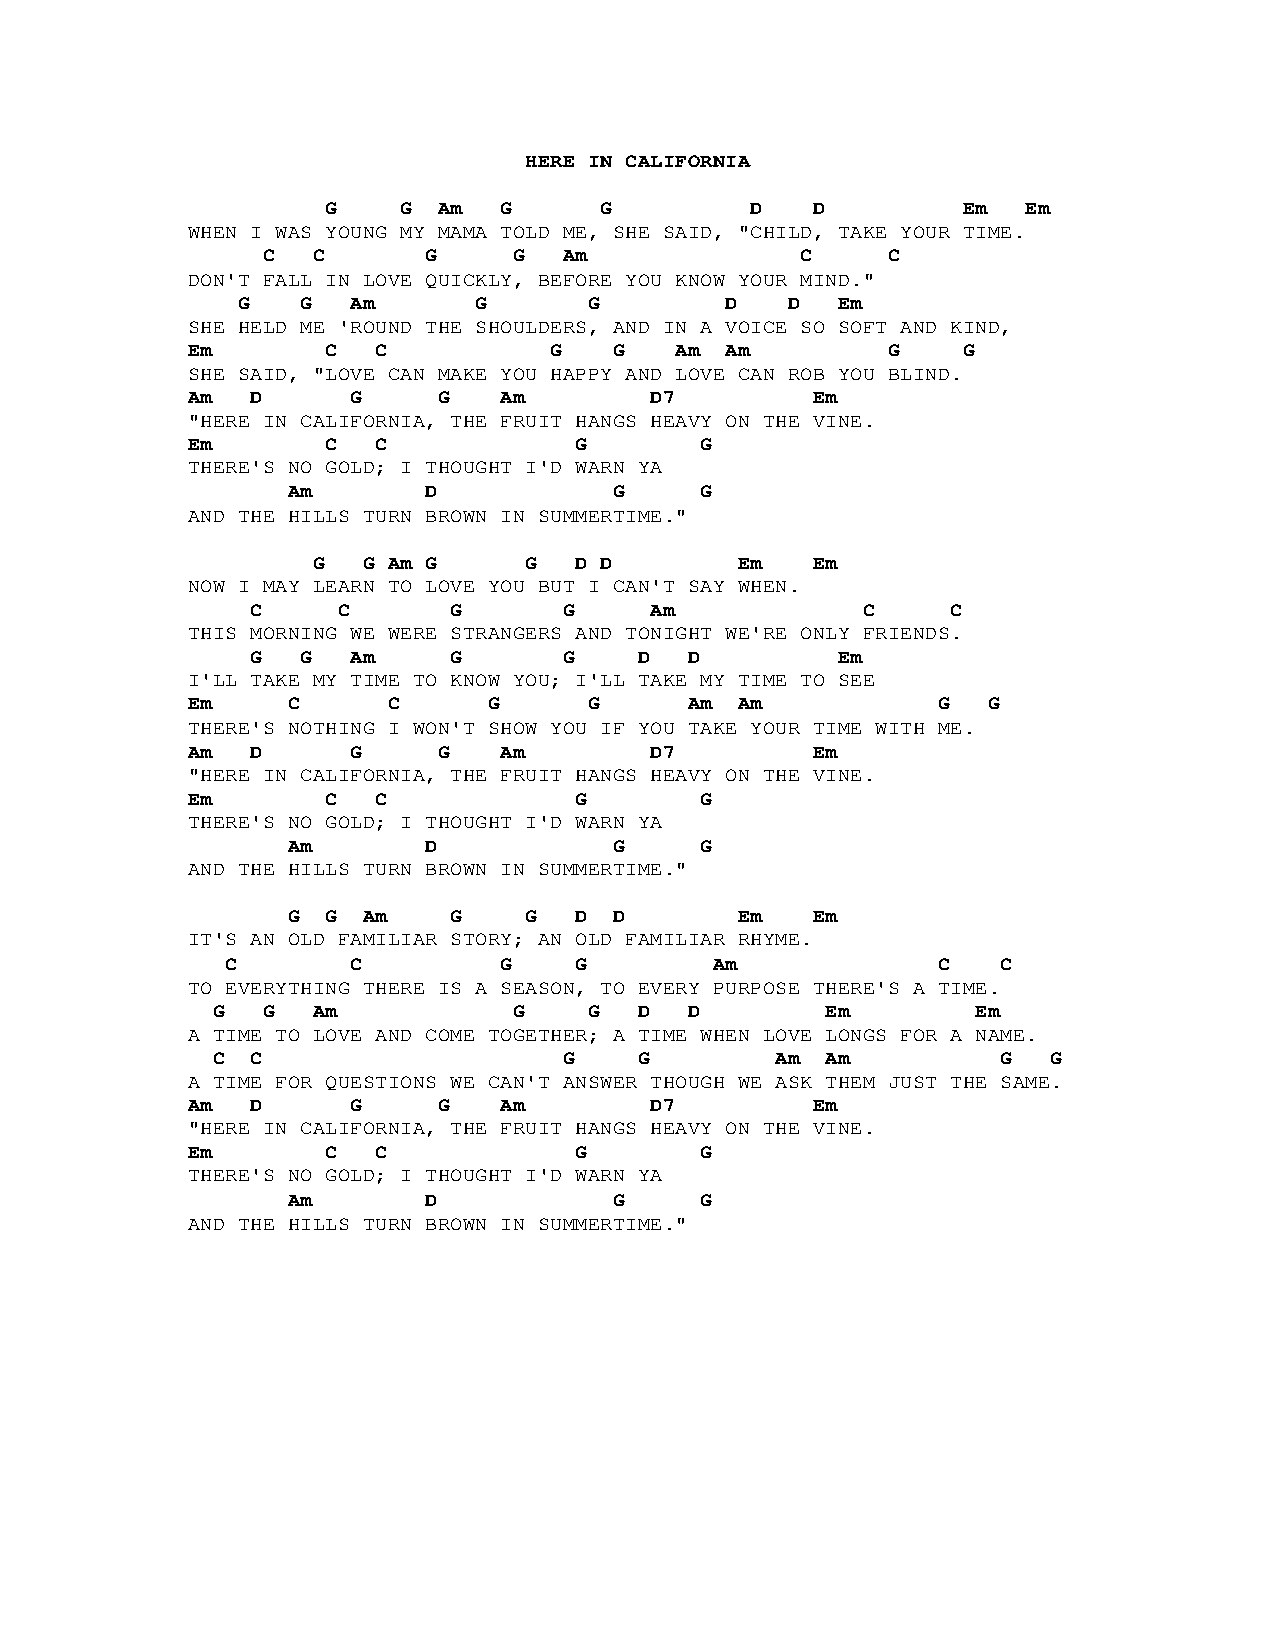
\includepdf[addtotoc={275, chapter, 1, Here in California, p1}]{here_in_california.pdf}

\chapter{Long Journey Home}
\begin{verbatim}
G                       
Lost all my money but a two-dollar bill 
G                       C
Two-dollar bill, boys, two-dollar bill
G
Lost all my money but a two-dollar bill
          D            G
I'm on my long journey home
 
Well, black smoke's a-rising and it surely is a train 
Surely is a train, boys, surely is a train 
Black smoke's a-rising and it surely is a train 
I'm on my long journey home 
 
 
There's pretty girls a-waiting on down the line 
On down the line, Lord, on down the line 
There's pretty girls a-waiting on down the line 
And I?m on my long journey home 
 
 
Well I'm homesick and lonesome and feeling kind of blue 
Feeling kind of blue, boys, feeling kind of blue 
Homesick and lonesome and I'm feeling kind of blue 
And I'm on my long journey home 
 
Cloudy in the west and it looks like rain
Looks like rain boy, looks like rain.
Cloudy in the west and it looks like rain
I'm on my long journey home.

It's starting raining and I've got to go home
I've got to go home boys, I've got to go home
It's starting raining and I've got to go home
I'm on my long journey home.Long
 
Lost all my money but a two-dollar bill 
Two-dollar bill, boys, two-dollar bill 
Lost all my money but a two-dollar bill 
And I'm on my long journey home 
 
Chorus 
     
\end{verbatim}
\newpage


\chapter{The Hills that I call Home}
\begin{verbatim}
The Hills That I Call Home
Recorded by Front Range
Album: Back To Red River (2006)

Intro.:  |(Am) |(Am) |(C) |(C) |(G) |(G) |(C) |(C)

I was (C)born (G) upon a (C)hillside
Where the (F)pines sing in the (C)wind
Where my daddy (E/B)lived be-(Am)fore me
And my (G)grandpa before (C)him

We be-(C)lieve (G) in simple (C)livin'
It's the (F)only life we (C)know
All we (C)need here (E/B)is our (Am)freedom
And a (G)place to call our (C)own

(Chorus)
In the (Am)land of Ethan (C)Allen
Where the (G)sugar maples (C)grow
Where the wild grass (C/B)fills the (Am)meadows
And the (G)rocky rivers (Am)flow
By the (G)hills that I call (C)home

Inst.:  |(C) |(C) |(C) |(C) |(F) |(F) |(C) |(C) |
        |(C) |(C)(C/B)|(Am) |(Am) |(G) |(G) |(C) |(C)

Now I have (C)trav-(G)eled cross the (C)country
And there is (F)much that I have (C)learned
Still I felt no (E/B)peace in-(Am)side me
Till the (G)day that I re-(C)turned

For there're (C)two (G) things you can (C)count on
In this (F)troubled world we (C) face
Every season (E/B)has an (Am)ending
Every (G)person has a (C)place

Repeat Chorus

Outro.:  |(Am) |(Am) |(C) |(C) |(G) |(G) |(C) |(C) -----
\end{verbatim}
\newpage

\chapter{Green rolling hills}
\begin{verbatim}
Green rolling hills
Emmylou Harris
    C                   G               C
    The green rolling   hills of West   Virginia
        F                               G
Are the nearest thing to heaven that I  know
        C
Tho the times are sad and drear
        F
And I   cannot linger here
            C           G           C
They'll     keep me and never let me go
    C                   G           C
    My daddy said don't ever be a   miner
        F                                 G
For a   miner's grave is all you'll ever own
            C
'Cause the  hard times everywhere
    F
I   can't find a dime to spare
    C                   G               C
    These are the worst times I've ever known
    C                   G               C
    The green rolling   hills of West   Virginia
        F                               G
Are the nearest thing to heaven that I  know
        C
Tho the times are sad and drear
        F
And I   cannot linger here
        C           G            C
They'll keep me and never let me go

    C                    G               C
    So I'll move away in to some crowded city
            F                                   G
In some     northern factory town you'll find me there
            C
Tho I'll    leave the past behind
        F
I'll    never change my mind
        C                   G               C
These   troubled times are  more than I can bear

    C                   G               C
The green rolling   hills of West   Virginia
            F                               G
Are the     nearest thing to heaven that I  know
            C
Tho the     times are sad and drear
        F
And I   cannot linger here
            C           G            C
They'll     keep me and never let me go

SOLO

        C               G               C
    But someday I'll go back to West    Virginia
        F                               G                       
To the  green rolling hills I love so   well
        C
    Yes, someday I'll go home
        F
And I   know I'll right the wrong
        C                   G             C
These   troubled times will follow me no more
    C
    Yes, someday I'll go home
        F
And     I know I'll right the wrong
        C                   G               C   G   C
These   troubled times will follow me no    more            
\end{verbatim}
\newpage

\chapter{Yuba City}
\begin{verbatim}
G                   D
I came into Yuba as soon as I read
D                           G
Of all of those twenty-five hobos found dead,
G                        C
I came in to find out if one of the slain
G                       D           G
Could have answered to my brother's name.
G                           D
It might be your brother, I just couldn't say,
D                           G
We hire lots of floaters who work by the day;
G                        C
Now I see his photo they might be the same,
G                   D       G
But I never did ask him his name.
G                             D
If I had a list and if I only knew,
D                                           G
I'd write down their names and sing them to you,
G                                   C
And when I got done, I'd sing them again,
G                       D         G
So you'd all know each one had a name.

He had a room and ran out on the rent,
Hired on a crew, I don't know where he went,
If I knew his boss, I might make a claim,
But I never did write down his name.

He stopped for a drink every now and again,
Didn't look no different than hundreds of men;
You know these old bums, they all look the same,
No reason to ask him his name.

It might have been Shorty, a feller I knew,
We bunked in the empties when the season was through.
You know, I been thinking, it sure is a shame
I never did ask him his name.

We always abandon the old for the new,
And second-hand people get thrown away, too;
I know it won't help, but still it explains
Why no one remembers their names. 
\end{verbatim}
\newpage



\chapter{Walking Through your Town in the Snow}
\begin{verbatim}
        D                 A         D
I'm walking through your town in the snow
                          A        D
I'm walking through your town in the snow
  G                  
I've got no place to go –
                           D
All the trains are running slow
        D                    A            D
And I'm walking through your town in the snow

  D                       A               D
It's getting late and all the bars are closed
  D                       A               D
It's getting late and all the bars are closed
   G                 
I'm so cold I can't think –
                     D
I could really use a drink
   D                  A                   D
And I'm walking through your town in the snow

                               A                  D
Don't all these little winter towns all look the same
                               A                  D
Don't all these little winter towns all look the same
     G
How the freezing winds they blow
                           D
When the mission doors are closed
     D                       A           D
Now I'm walking through your town in the snow

  D           A        D
I carry my home on my back
  D           A         D
I carry my home on my back
        G            
But the police only frown
                     D
Every time I lay it down
                            A                 D
And I'm walking through your town in the snow

                           A             D
There's some fellows jungled up by the yard
                           A              D 
There's some fellows jungled up by the yard
     G
They're cooking up down there
                       D
And I've nothing left to share
                      A                   D
And I'm walking through your town in the snow

               A        D
Maybe I can rustle up a job
               A        D 
Maybe I can rustle up a job
         G
But there's nothing I can do
                          D  
My best working days are through
                        A               D
And I'm walking through your town in the snow

                           A           D
Don't ever think I'll find my way back home
                           A           D
Don't ever think I'll find my way back home
  G
I can see my golden years
                              D
Shining through these golden tears
    D                     A             D
And I'm walking through your town in the snow

                          A            D
I'm walking through your town in the snow
                          A            D
I'm walking through your town in the snow
   G
I've got no place to go –
                         D    
All the trains are running slow
                             A           D
And I'm walking through your town in the snow 
\end{verbatim}
\newpage



\chapter{Corn Bread and Butterbeans}
\begin{verbatim}
Chorus:
G                                            C
Cornbread and butterbeans and you across the table
D                                                 G
Eating them beans and making love as long as I am able
G                                               C
Growing corn and cotton too and when the day is over
D                                                 G
Ride the mule and cut the fool and love again all over

G                                        C
Goodbye don't you cry I'm going to Louisiana
D                                             G
Buy a coon dog and a big fat hog and marry Suzianna.
G                                       C
Same song ding dong I'll take a trip to China
D                                              G
Cornbread and butterbeans and back to North Carolina.

REPEAT CHORUS

G                                                 C
Wearin' shoes and drinkin' booze goes against the Bible.
D                                                   G
A necktie will make you die and cause you lots of trouble
G                                                 C
Streetcars and whiskey bars and kissing pretty women
D                                         G
Women yeah that's the end of a terrible beginning

REPEAT CHORUS

G                                              C
I can't read and don't care and education is awful
D                                                   G
Raisin' heck and writing checks it ought to be unlawful
G                                                 C
Silk hose and frilly clothes is just a waste of money
D                                                   G
Come with me and stay with me and say you'll be my honey

REPEAT CHORUS
\end{verbatim}
\newpage



\chapter{The Real old Mountain Dew}
The Chocolate Drops mostly just play G with a little Em now and again.
\begin{verbatim}
                     G                         C
Hay da diddle diddle doo, hay da diddle diddle day, 
       G                  D
Hay da diddle did doo dal day
                     G                         C
Hay da diddle diddle doo, hay da diddle diddle day
       G          D       G
Hay da diddle did doo dal day


    G                C                G             D
Let grasses grow and waters flow in a free and easy way
    G                     C                     G         D      G
But give me enough of the rare old stuff that's made near Galway Bay
     G                                                Em
Come gaugers all from Donegal, from Sligo and Leitrim too
      G                            C                 G        D        G
We'll give them the slip and we'll take a sip of the real old Mountain Dew

Chorus:

At the foot of the hill there's a neat little still, where the smoke curls up the sky
By a whiff of the smell you can plainly tell, there's a poitin still close by
Oh it fills the air with a perfume rare and betwixt both me and you
As home we roll, we can drink a bowl or a bucket of Mountain Dew
Chorus:

Now learned men who use the pen have wrote the praises high
Of the sweet poitin from Ireland green, destilled from wheat and rye
Away with pills, it will cure all ills of the Pagan, Christian or Jew
So take off your coat and grease your throat with the real old Mountain Dew

Chorus:
\end{verbatim}
\newpage

\chapter{Falling Slowly}
\begin{verbatim}
#------------------------------------------------------------------#
Falling Slowly chords
Marketa Irglova & Glen Hansard  *


C F Am F 3x

C                F
I don t know you but I want you
C                F
All the more for that
C                     F
Words fall through me and always fool me
C             F
And I can t react

Am         G      F        G               Am
Games that never amount to more than their meant
     G               F 
Will play themselves out

C         G       Am       G        F
Take this sinking boat and point it home
      C         G  F
We ve still got time
C          G       Am        G      F
Raise your hopeful voice you have a choice
       C       G   F
You ve make it known

C               F 
Falling slowly, eyes that know me
C              F
And I can t go back
C                  F
Moods that take me and erase me
C               F
And I m painted black

Am       G         F         G               Am
You have suffered enough and warred with yourself
     G             F
It s time that you won

C         G       Am       G        F
Take this sinking boat and point it home
      C         G  F
We ve still got time
C          G       Am        G      F
Raise your hopeful voice you have a choice
       C       G   F
You ve make it known
C       G       Am        G
Falling slowly, sing your melody
F    C       G  F
I ll sing it loud

C G Am G F C G F 3x

* Alternate:


Capo III

C  = A
F  = D
Am = F#m
G  = E

\end{verbatim}
\newpage

\chapter{Nothing Better}
Capo 2nd fret to match recording
\begin{verbatim}
Intro
-----

C - F - Am - G - F - Am - G - G(7)
C - F - Am - G - F - Am - G - G(7)


Verse
-----
                           C
Will someone please call a surgeon
        F                   Am                     G
Who can crack my ribs and repair this broken heart
               F                           G     (G7)
That your're deserting for better company?


                         C
I can't accept that it's over...
       F                     Am                     G
I will block the door like a goalie tending the net
               F                            G    (G7)
In the third quarter of a tied-game rivalry


Chorus
------

   C          F                G     Em
So,  just say how to make it right
    C              F                G   Em
And,  I swear I'll do my best to comply


Am      F      G                       C                 Am
Tell me am I right to think that there could be nothing better
     Am     F       G               Em          Am
Than making you my bride and slowly growing old together

C - C - C - C


Verse
-----
                 C                        F                    Am       
I feel must interject here you're getting carried away feeling sorry for
     G                 F                        G    (G7)
yourself With these revisions and gaps in history
                     C
So let me help you remember
          F                             Am                G
I've made charts and graphs that should finally make it clear
                  F                         G    (G7)
I've prepared a lecture on why I have to leave


Chorus
------

   C              F               G    Em
So,  please back away and let me go
C            F                   G        Em
  I can't my darling I love you so...  Oh oh


Am      F      G                       C                 Am
Tell me am I right to think that there could be nothing better
     Am     F       G               Em          Am
Than making you my bride and slowly growing old together

Am        F        G               C           Am
Don't you feed me lines about some idealistic future
Am         F           G                Em              Am
Your heart won't heal right if you keep tearing out the sutures

Am / F - G - C - Am
Am / F - G - Em - Am

Am / F - G - C - Am
Am / F - G - Em - Am








Outro
-----

C              F               Am   G     F
  I admit that I have made mistakes   and   I swear
                      G    (G7)
I'll never wrong you again

C              F               Am    G
  You've got a lure I can't deny,
    F                                    G    (G7)
But   you've had your chance so say goodbye
        C
Say goodbye
\end{verbatim}
\newpage





\chapter{Horchata}
Drop C, maybe with capo and falsetto?
\begin{verbatim}

C    F       G          C
in december drinking horchata
C           F          G    C
I'd look psychotic in a balaclava
F                 G          C
winter's cold is too much to handle
F                   G            C
puncher crabs that pinch at your sandals

C       C       C       C 
aaah ah aaah ah aaah ah aaah
C       F       G       C
(instrumental)
C       C       C       C 
aaah ah aaah ah aaah ah aaah
C       F       G       C
(instrumental)

C    F       G          C
in december drinking horchata
C              F             G     C
look down your glass at that aranciata
F                      G          C
with lips and teeth to ask how my day went
F                  G            C
boots and fists to pound at the pavement

F9/C                       G6
here comes the feeling you thought you'd forgotten
F9/A               G6/B        C 
chairs to sit and sidewalks to walk on

C       C       C       C 
aaah ah aaah ah aaah ah aaah
C       F       G       C

C       C       C       C 
aaah ah aaah ah aaah ah aaah
C       F       G       C


C    F       G          C
you'd remember drinking horchata
C           F          G    C
you'd still enjoy it with your foot on masada
F                 G          C
(instrumental)
F                 G          C
(instrumental)

F                 G          C
winter's cold is too much to handle
F                   G            C
puncher crabs that pinch at your sandals

F9/C                       G6
here comes the feeling you thought you'd forgotten
F9/A               G6/B        C
chairs to sit and sidewalks to walk on
F9/C                 G6
ooh you had it but oh no you lost it
F9/A               G6/B        C
chairs to sit and sidewalks to walk on 

C     C     G7     C
(instrumental)
C     C     G7     C
(instrumental)
C     C     G7     C
(instrumental)
C     C     G7     C
(instrumental)















C    F       G          C
in december drinking horchata
C           F          G    C
I'd look psychotic in a balaclava
F                 G          C
winter's cold is too much to handle
F                   G            C
puncher crabs that pinch at your sandals
F                 G             C
years go by and hearts start to harden
F                         G            C
those palms and firs that grew in your garden
F                    G           C
are falling down and nearing the rose beds
F                     G               C
the roots are shooting up through the tool shed
F                 G          C
those lips and teeth that asked how my day went
F                   G            C
are shouting up through cracks in the pavement

F    F    G    C
(instrumental)

F9/C                       G6
here comes the feeling you thought you'd forgotten
F9/A               G6/B        C
chairs to sit and sidewalks to walk on
F9/C                 G6
ooh you had it but oh no you lost it
F9/A               G6/B        C
you understood so you shouldn't have fought it

F9/C                       G6
here comes the feeling you thought you'd forgotten
F9/A               G6/B        C
chairs to sit and sidewalks to walk on
F9/C                 G6
ooh you had it but oh no you lost it
F9/A               G6/B        C
chairs to sit and sidewalks to walk on. 

\end{verbatim}
\newpage


\chapter{We will Become Silhouettes (Shins version)}
\begin{verbatim}
Into:
A  D (5x)

A
              A                    D
I've got a cupboard with cans of food, 
           A                     D
filtered water, And pictures of you 
         A                    D
and I'm not coming out until this is all over

A  D

         A                    D                       
And I'm looking through the glass 
           A                   D
where the light bends at the cracks
             A                       D                  
And I'm screaming at the top of my lungs pretending
      A                D                                       
The echoes belong 


Pre Chorus:
        Bm       D
to someone 
                                                   
Someone I used to know

A  D


Chorus:
         Bm       E
And we become 

silhouettes when our bodies finally go

A  D  (5x)

A



Verse 2:
             A                      D
I wanted to walk through the empty streets
                     A                D
And feel something constant under my feet,
            A                      D                A     D
But all the news reports recommended that I stay indoors
            A                 D
Because the air outside will make 
            A                    D
our cells divide at an alarming rate 
            A                         D
until our shells simply cannot hold all our insides in,
            A                   D
And that's when, (that's when), that's when


Pre Chorus:
           Bm        D
we'll explode

and it won't be a pretty sight

A  D  


Chrorus:
           Bm        E
And we'll become 

silhouettes when our bodies finally go


A  D  (10x) (la la la la la)

Bm  E

\end{verbatim}
\newpage


\chapter{Kissing the Lipless}
\begin{verbatim}
Intro
C  D  C  D


C          D           C        D
Called to see If your back was still aligned

          C          D                         C             D 
And your sheets Were growing grass all on the corners of your bed

     C             D                    C
But you've got too much to wear on your sleeves 

         D                   C     D                 C              D
that has too much to do with me and secretly I want to bury in the yard

    Em               F          C     D
The grey remains of a friendship scarred


    C               D                     C                D
You told us of your new life there you got someone coming 'round

         C                D               C               D
Glueing tinsel to your crown he's got you talkin' pretty loud

       C   D             C                     D
you berate remember your ailing heart and your criminal eyes

    C                     D         C                   D
You say you're still in love if it's true, what can be done?

     Em                     F         C   D
It's hard to leave all these moments behind










C          D           C        D
Called to see If your back was still aligned

          C          D                         C             D 
And your sheets Were growing grass all on the corners of your bed

     C             D                    C
But you've got too much to wear on your sleeves 

         D                   C     D                 C              D
that has too much to do with me and secretly I want to bury in the yard

    Em               F          G
The grey remains of a friendship scarred



    C           D        C            D
You tested your mettle on doe skin and petals

    C           D          C             C#         Em  F  C  C#
And kissing the lipless you bleed all the sweetness away


Outro

C  D  Em  F    Reapeted A# few times

Finish: C  D  Em  F  G
\end{verbatim}
\newpage


\chapter{Gone For Good (The Shins)}
\begin{verbatim}

Untie me, I've said no vows
C
The train is getting way too loud
         F
I gotta leave here my girl
                C
Get on with my lonely life
               G
Just leave the ring on the rail
                       C
For the wheels to nullify

C
Until this turn in my head
C
I let you stay and you paid no rent
        F                          C
I spent twelve long months on the lam
              G
That's enough sitting on the fence
                        C
For the fear of breaking dams


Am       C
I find a fatal flaw
       F
In the logic of love
       C          G     Am
And go out of my head

           C
You love a sinking stone
        F
That'll never elope
       C           G
So get used to the lonesome
       C          G
Girl, you must atone some
       C          G            F        C
Don't leave me no phone number there

(Solo): C/C/F/C/G/C

C
It took me all of a year
C
To put the poison pill to your ear
          F                          C
But now I stand on honest ground, on honest ground
            G
You want to fight for this love
              F
But honey you cannot wrestle a dove
            C
So baby it's clear


Am          C
You want to jump and dance
       F
But you sat on your hands
         C                 G
And lost your only chance
Am          C
Go back to your hometown
         F
Get your feet on the ground
         C         G
And stop floating around

Am       C
I find a fatal flaw
       F
In the logic of love
       C          G     Am
And go out of my head

           C
You love a sinking stone
        F
That'll never elope
       C                   G
So get used to used to the lonesome
       C          G
Girl, you must atone some
       C          G            F         C
Don't leave me no phone number there
\end{verbatim}
\newpage


\chapter{Peace Train}
\begin{verbatim}
    C    G    C
Now I've been happy lately, 
F         C        F
thinking about the good things to come
    G   Am 
And I believe it could be, 
F         G    F
something good has begun

   C    G    C
Oh I've been smiling lately, 
F         C        F
dreaming about the world as one
    G   Am
And I believe it could be, 
F    G        F
some day it's going to come

      C   G      C
Cause out on the edge of darkness, 
F     C       F
there rides a peace train
         G     Am
Oh peace train take this country, 
F    G       F
come take me home again

    C    G    C
Now I've been happy lately, 
F         C        F
thinking about the good things to come
    G   Am 
And I believe it could be, 
F         G    F
something good has begun

   C     G     C        G  C
Oh peace train sounding louder
F     C      F
Glide on the peace train
F    G  Am
Come on now 
F    G      F
come on the peace train

C     G     C    G  C  
peace train holy roller
F        C             F
Everyone jump upon the peace train
F   G   Am
oooooooooo
F       G   F
Come on now peace train

Get your bags together, 
go bring your good friends too
Cause it's getting nearer, 
it soon will be with you

Now come and join the living, 
it's not so far from you
And it's getting nearer, 
soon it will all be true

Now I've been crying lately, 
thinking about the world as it is
Why must we go on hating, 
why can't we live in bliss

Cause out on the edge of darkness, 
there rides a peace train
Oh peace train take this country, 
come take me home again

\end{verbatim}
\newpage



\chapter{I Want to Live in a Wigwam}
\begin{verbatim}
VERSE 1

G                         D (Dsus4)
   I'd like to live in a wigwam. 
     Bm7                   Am
Yes, I'd like to live in a wigwam.
(Am)         D         G   C
I'd like to live in a wig-wam, 
     D                     Em   Riff 1
And dance round the totem pole. 

VERSE 2

G                          D (Dsus4)
   I'd like to live in an igloo. 
     Bm7                     Am
Yes, I'd like to live in an igloo.
(Am)         D          G    C
I'd like to live in an igloo-oo,
     D                Em    Riff 2
And fish from an ice-hole.


VERSE 3

         G                 D (Dsus4)
Oh, I'd like to ride on a caravan.
     Bm7                      Am
I'd like to take a ride on a cara-van.
     (Am)         D         G   C
Yes, I'd like to ride on a cara-van, 
     D                 Em   Riff 1
And sing with the gyp-sies.

VERSE 4
G                         D (Dsus4)
   I'd like to live on a commune.
     Bm7                    Am
Yes, I'd like to live on a commu-une.
(Am)         D         G    C
I'd like to live on a commu-une,
     D                    Em     Riff 2
And people can call me a hippie.


INTERLUDE

| G | D7/F# (D7sus4/F#) | Bm7 | Em | 

| Am Asus4 | D | Am7 (A7sus4) D | 

|: A7sus4 A7sus2 Am7 :| (x2)

| D Am B/F# | Em | Riff 2 |


VERSE 5
   G                       D (Dsus4)
I don't want to live in a palace.
   Bm7                          Am
No, I don't want to live in no palace.
   (Am)              D          G    C
Oh, I don't want to live in no pala-ace.
         D               Em     Riff 2
There's too many empty rooms. 


VERSE 6
       G                       D (Dsus4)
And I don't want to live in a barracks,
      Bm7                Am
Don't want to live in a barracks.
   (Am)              D          G    C
Oh, I don't want to live in a barra-acks,
     D                    Em     Riff 1
And wake up to the bugle tune.


VERSE 7
     G                      D (Dsus4)
I'd just like to live on a tree hut. 
     Bm7                    Am
Yes, I'd like to live on a tree hu-ut.
    (Am)          D         G      C
Yes, I'd like to live on a tree hu-ut,
     D                          Em     Riff 2
And listen to the sound of the birds.



VERSE 8
   G                       D (Dsus4)
I don't want to live in a jailhouse. 
       Bm7                      Am
Don't wanna bide my time in no jailhouse. 
   (Am)              D          G      C
No, I don't want to live in no jailhou-use,
    D                         Em     Riff 2
And be fed bread through the bars.


OUTRO
     C/G
I'm glad I'm alive am I,
     F/C              G
I'm glad I'm alive am I, 
     F/C        C/G
I'm glad I'm a-live,
     F/C        C/G
I'm glad I'm a-live,
     F/C              G
I'm glad I'm alive am I.

    C/G
We gotta get our heads up in the sky,
    F/C                           G
We gotta get our heads up in the sky,
    F/C           C/G
We gotta get our heads up,
 F/C   Em/B  Am
Gotta give a try,
    F/C                           G
We gotta get our heads up in the sky.

    C/G
We gotta get to Heaven, get a guide, 
    F/C                        G
We gotta get to Heaven, get a guide,
    F/C         C/G
We gotta get a Heaven,
    F/C          C/G
We gotta have a guide, 
    F/C                       G      Em
We gotta get a Heaven, get a guide_______.
\end{verbatim}
\newpage



\chapter{Us}
\begin{verbatim}

Us - Regina Spektor


(CAPO 1st Fret)


INTRO:     C        F         C          F  (x2)


C           F         C            F
They made a statue of us
C           F             C            F
Then put it on a mountain top
C            F                 C            F
The tourists come and stare at us
     C                  F
Blow bubbles with their gum
     C                F         C        F        C        F
Take photographs have fun, have fun


C              F          C            F
They'll name a city after us
C         F                C            F
And later say it's all our fault
C                      F
Then they'll give us a talking to
C                      F
Then they'll give us a talking to
C                 F             C          F
Cause they've got years of experience


      C          F              Am       G
We're liiiiiiiiiiiiiiiiiving in a den of theives
C            F              Am   G
Rumaging for answers in the pages
      C          F              Am       G
We're liiiiiiiiiiiiiiiiiving in a den of theives
C           F
And its contagious
Am          G
And its contagious
C           F
And its contagious
Am          G           C         F         C          F
And its contagious


C           F                   C            F
We wear our scarves just like a noose
C                F            C            F
But not cause we want eternal sleep
C              F                 C            F
And though our parts are slighty used
C            F                   C            F
New ones are slave labor you can keep


      C          F              Am       G
We're liiiiiiiiiiiiiiiiiving in a den of theives
C            F              Am   G
Rumaging for answers in the pages
      C          F              Am       G
We're liiiiiiiiiiiiiiiiiving in a den of theives
C           F
And its contagious
Am          G
And its contagious
C           F
And its contagious
Am          G           C         F         C          F
And its contagious


C           F         C
They made a statue of us
            F         C
They made a statue of us
             F                 C
The tourists come and stare at us
              F             C
The sculptors mama sends regards
            F         C
They made a statue of us
            F         C
They made a statue of us
          F             C
Our noses have begun to rust


      C          F              Am       G
We're liiiiiiiiiiiiiiiiiving in a den of theives
C            F              Am   G
Rumaging for answers in the pages
      C          F              Am       G
We're liiiiiiiiiiiiiiiiiving in a den of theives
C           F
And its contagious
Am          G
And its contagious
C           F
And its contagious
Am          G           C         F         C          F
And its contagious
\end{verbatim}
\newpage


\chapter{Summer in the City}
\begin{verbatim}

C                        F
Summer in the city means cleavage cleavage cleavage
C                              G
And I start to miss you, baby, sometimes          
          C              G              C         F
I've been staying up and drinking in a late night establishment
C                 G
Telling strangers personal things

C                          F
Summer in the city, I'm so lonely lonely lonely
C                                             G
So I went to a protest just to rub up against strangers
      C             G            C              F
And I did feel like coming but I also felt like crying
C                           G
It doesn't seem so worth it right now

F                                          C
And the castrated ones stand in the corner smoking
F                                     C              G
They want to feel the bulges in their pants start to rise
        C        G               C         F
At the site of a beautiful woman they feel nothing but
C                                            G
Anger, her skin makes them sick in the night nauseaous, nauseaous, nauseaous

C                          F
Summer in the city, I'm so lonely lonely lonely
            C                                             G
I've been hallucinating you, babe, at the backs of other women
      C            G               C             F
And I tap on their shoulder and they turn around smiling
           C                       G
But there's no recognition in their eyes








C                           F      
Oh summer in the city means cleavage cleavage cleavage
C                                                        G
And don't get me wrong, dear, in general I'm doing quite fine
                    C             G               C                      F
It's just when it's summer in the city, and you're so long gone from the city
   C                 G     C
I start to miss you, baby, sometimes

INSTRUMENTAL

          C             G
When it's summer in the city
              C                  F
And you're so long gone from the city
C                    G     F
I start to miss you, baby, sometimes
C                    G     F
I start to miss you, baby, sometimes
C                    G     F
I start to miss you, baby, sometimes
\end{verbatim}
\newpage


\chapter{Two Birds}
\begin{verbatim}
C   G          Am Em
Two birds on a wire
F          G    F
One tries to fly away
        G
And the other
C           G
Watches him close
          Am Em
From that wire
F                     G
He says he wants to as well
F       G
But he is a liar

C               G   C
I'll believe it all
        Am        F     G
There's nothing I won't understand
C               G   C
I'll believe it all
  Am        F        G
I won't let go of your hand

C   G          Am Em
Two birds on a wire
F       G
One says come on
F
And the other says
G
I'm tired
C          G
The sky is overcast
        Am  Em
And I'm silent
F               G
One more or one less
F     G
Nobody's worried




C               G   C
I'll believe it all
Am                F         G
There's nothing I won't understand
C               G    C
I'll believe it all
Am          F         G
I won't let go of your hand

C   G          Am Em
Two birds of a feather
F               G
Say that they're always
F          G
Gonna stay together
C                G
But one's never goin' to
    Am          Em
Let go of that wire
F              G
He says that he will
F             G
But he's just a liar

C   E          Am E
Two birds on a wire
F           G   F
One tries to fly away
        G
And the other
C           E
Watches him close
          Am E
From that wire
F                     G
He says he wants to as well
F        G
But he is a liar

C   G          Am Em
Two birds on a wire
F           G   F
One tries to fly away
         G
And the other
\end{verbatim}
\newpage




\chapter{My Little Armalite}
\begin{verbatim}
I was [G] stopped by a soldier he called me a Fenian swine
He [D] hit me with his rifle and he [G] kicked me in the [D] groin
I [G] begged and [C] pleaded told him [G] that I wouldn`t [D] fight
But sure [G] all that I could [Em] think of was my [D] little arma[G]lite

[chorus]
And it`s down in the Bogside that`s where I want to be
Lying in the dark with a Provo company
A comrade on my left and another one on my right
And a clip of ammunition for my little armalite

Well a brave RUC man came walking down our street
Six hundred British soldiers he had lined up at his feet
Come out you cowardly Fenians come on out and fight
But he cried I`m only joking when he heard our armalites

And its up along the Falls Road...

Now the Brits came to visit me twas in the early hours
With Saracens and Saladans and great big armoured cars
They thought they had me covered but I gave them all a fright
With the armour-piercing bullets from my little armalite

And it`s down in the New Lodge...

When big Harry came to Belfast he said the battles won
The generals had all told them that we were on the run
Their coorporals and privates went on patrol one night
They cried send home for reinforcements its those bloody armalites

And it`s out in Crossmaglen...

And it`s down in old Andy` town...
\end{verbatim}
\newpage


\chapter{Old Joe Clark}
Chords are G and F, listen for the changes.
\begin{verbatim}
Old Joe Clark's a fine old man
Tell you the reason why
He keeps good likker 'round his house
Good old Rock and Rye

Chrous:
Fare ye well, Old Joe Clark
Fare ye well, I say
Fare ye well, Old Joe Clark
I'm a going away

Round and Round, Old Joe Clark
Round and Round I say
I've come about ten thousand miles
to hear your banjo play

Old Joe Clark, the preacher's son
Preached all over the pain
The only text he ever knew
Was High, low, Jack and the game

Old Joe Clark had a mule
His name was Morgan Brown
And every tooth in that mule's head
Was sixteen inches around

Old Joe Clark had ayellow cat
She would neither sing or pray
She stuck her head in the butermilk jar
And washed her sins away

Old Joe Clark had a house
Fifteen stories high
And every story in that house
Was filled with chicken pie

I went down to Old Joe's house
He invited me to supper
I stumped my toe on the table leg
And stuck my nose in the butter


Now I wouldn't marry a widder
Tell you the reason why
She'd have so many children
They'd make those biscuits fly

Sixteen horses in my team
The leaders they are blind
And every time the sun goes down
There's a pretty girl on my mind

Eighteen miles of mountain road
And fifteen miles of sand
If ever travel this road again
I'll be a married man

Never Marry and old school teacher
Tell you the reason why
Blow her nose in old corn bread
and call it pumkin pie



\end{verbatim}
\newpage

\chapter{Holocene}
\begin{verbatim}
C                    C            Am        G    
Someway, baby, it's part of me, apart from me.
        Am             F
you're laying waste to Halloween 
   C                                         Am             G
you fucked it friend, it's on it's head, it struck the street 
       Am             F
you're in Milwaukee, off your feet 


         F                                     Am   G   
and at once I knew I was not magnificent 
F                                Am  G
strayed above the highway aisle 
 F      Am        C           G
jagged vacance, thick with ice 
                Am       F      G     C   
I could see for miles, miles, miles 


C                                 Am  G
3rd and Lake it burnt away, the hallway 
    Am                  F
was where we learned to celebrate 
C                                Am       G
automatic bought the years you'd talk for me 
     Am                F
that night you played me ?Lip Parade? 
C                                   Am   G
not the needle, nor the thread, the lost decree 
       Am               F
saying nothing, that's enough for me 


       F                                   Am   G
And at once I knew I was not magnificent 
F                                 Am  G
hulled far from the highway aisle 
  F      Am         C        G
jagged, vacance, thick with ice
                Am      F      G     C
I could see for miles, miles, miles 


C                                       Am             G
Christmas night, it clutched the light, the hallow bright 
C                     G
above my brother, I and tangled spines 
                                         Am     G
we smoked the screen to make it what it was to be 
       Am              F
now to know it in my memory: 

 
        F                               Am     G
And at once I knew I was not magnificent 
 F                           Am  G
high above the highway aisle 
 F       Am       C          G
jagged vacance, thick with ice 
                Am     F      G     C
I could see for miles, miles, miles
\end{verbatim}
\newpage


\chapter{Let My Love Open the Door}
\begin{verbatim}
  C           G      F      G       C              G        F      G
When people keep repeating      That you'll never fall in love
  C      G               F   G      C                    G    F    G
When everybody keeps retreating   But you can't seem to get enough

 A m       G         F
Let my love open the door
 A m       G         F
Let my love open the door
 A m       G         F
Let my love open the door
To your heart  [C,G,F,G]

        C        G         F   G
When everything feels all over
When everybody seems unkind
I'll give you a four leaf clover
Take all the worry out of your mind

 A m        G        F
Let my love open the door
Let my love open the door
Let my love open the door
To your heart
 
Am (Strum)                               Dm (Strum)
I have the only key to your heart       I can stop you falling apart
F                                                           G
Release yourself from misery    Only one thing's gunna set you free
            C G F G
N’ that's my love
Let my love open the door
Let my love open the door          A
Let my love open the door to your heart
 
A m                 F              A m                    F
When tragedy befalls you          Don't let them bring you down
A m                   F            A m             F
Love can cure your problems  You're so lucky I'm around

 A m                 F
Let my love open the door
Let my love open the door              A
Let my love open the door    To your heart
\end{verbatim}
\newpage


\chapter{My Hands are Shaking}
\begin{verbatim}
     G             B7
My hands are shaking 
        C                 B7
from carrying this torch 
C                 D7          G    D7
carrying this torch for you 

     G         B7
My lips are bleeding
        C                     B7
from kissing you goodbye 
C                      D7           G      D7
kissing you goodbye every night 

      G             B7
My sheets are tearing
        C                    B7
from sleeping in too long
C                    D7          G    D7
sleeping in too long with you 

     G             B7
My hands are shaking 
        C                 B7
from carrying this torch 
C                 D7          G
carrying this torch for you 

[Chorus 1]
     Am       C#m
My head is where 
      F#m
it's always been 
          B7       E       E7
if only I knew where 

     Am    
My feet can't stand 
       E          G#m  C#m
that ground  no      more 
   G#m          F#m   B      C
It seems that I don't care 


[Verse 2]
     G             B7
My hands are shaking 
        C                 B7
from carrying this torch 
C                 D7          G    D7
carrying this torch for you 

     G         B7
My lips are bleeding
        C                     B7
from kissing you goodbye 
C                      D7           G     
kissing you goodbye every night

[Chorus 2]
     Am       C#m
My heart is pounding
F#m
yes yes yes 
             B7              E       E7
My mind just second guess 
    Am
My love is so 
E  G#m C#m
Ar -ti-   culate 
G#m F#m  B7    C
I am such a mess 

[Verse 3]
     G             B7
My hands are shaking 
        C                 B7
from carrying this torch 
C                 D7          G    D7
carrying this torch for you 

     G         B7
My lips are bleeding
        C                     B7
from kissing you goodbye 
C                      D7           G      D7
kissing you goodbye is all that I do 



     G             B7
My hands are shaking 
        C                 B7
from carrying this torch 
C                 D7          G   D7
carrying this torch for you

     G             B7
I said my hands are shaking 
        C                 B7
from carrying this torch 
C                 D7          G
carrying this torch for you 

[Ending]
G B7 C B7 C D7 G D7 
G B7 C B7 C D7 G

The end

Take the non Barré B7 to make like he does it… that means:

e|-2-----
B|-0-----
G|-2-----
D|-1-----
A|-2-----
E|-------
\end{verbatim}
\newpage


\chapter{Please Speak well of me}
\begin{verbatim}
C    F | C    F 

C              F
I've been away 
C                F
a year and a day
C                            F
You recognize love after the fact
C                                     F
You did what you did and that was that

Em        Am
Don't say words 
Em             Am
that you don't mean
Em             G                     | C     F | C     F
When I'm gone, please speak well of me

C                F
Looking back now
C                            F
I only wish I had been kinder
      C                               F
Did I ever know love, did I ever know love?
C                              F
And could I have been blinder?


Em        Am
Don't say words 
Em             Am
that you don't mean
Em             G                     | C     F | C     F
When I'm gone, please speak well of me
Em         Am
Don't hold back 
Em       Am
all your love 
F          | G
for someday, for someday




C                         F
I would say that I'm sorry 
C                       F
if it would do any good
C                                        F
But to never regret means you have to forget
C                              F
and I don't think that I could 

Em        Am
Don't say words 
Em             Am
that you don't mean
Em           | Em
When I'm gone, When I'm gone, 
Em             G                      | C    F
When I'm gone, please speak well of me

C    F | C    F | C   F | C

\end{verbatim}
\newpage



\chapter{I was Made for Sunny Days}
\begin{verbatim}
[G]                 [C]
I went to the market
[G]                                  [C]
though it was threatening rain
[G]                     [C]
I was late to the station
[G]                    [C]
so I missed that train
[G]                                 [C]
and the streets filled with umbrellas
[G]                         [C]
and we all look the same
[G]                            [C]
but I'm the one who's waiting
[D]
til the sun comes out again

chorus:
[C]              [D] [G]    [C]
I was made for sunny days
[C]              [D] [G]
I make do  with grey
        [C]
but I didn't stay
[C]              [D] [G]    [C]
I was made for sunny days
[C]              [D]       [G]
and I was made for you

verse:
[G]                          [C]
found the book you gave me
[G]                            [C]
when we were first in bloom
[G]                                      [C]
when I thougt that you might save me
[G]                                 [C]
from the dark side of the moon
[G]                            [C]
instead we both went walking to the
[G]                   [C]
shadows in the gloom
[G]                             [C]
and we never did stop talking
[D]
and you still light up the room
I say

chorus:
[C]              [D] [G]    [C]
I was made for sunny days
[C]              [D] [G]
I make do  with grey
        [C]
but I didn't stay
[C]              [D] [G]    [C]
I was made for sunny days
[C]              [D]       [G]
and I was made for you

bridge:
[G][C]    [G]      [C]
oooo the nights are longer
[G][C]    [G]    [C]
ooo you make me stronger
           [D]                              [C]
and the late light lingers on the grass
           [D]            [C]                       [D]
and the nights are dark but then they pass
[C]                        [D]
they don't seem so deep
[C]                  [D]                  [C]
I'm still losing sleep but I don't mind
[D]
I don't mind
i
verse:
[G]                      [C]
I got you a winter jacket
[G]                          [C]
that our baby wears around
           [G]                             [C]
and we chase him through the spring time
           [G]                           [C]
and the sleeves drag on the ground
      [G]                     [C]
and every hour we're working
     [G]                 [C]
and work and play are bound

      [G]                [C]
and every day is Sunday
              [D]
cause the sun comes dancing down
I say

chorus:
[C]              [D] [G]    [C]
I was made for sunny days
[C]              [D] [G]
I make do  with grey
        [C]
but I didn't stay
[C]              [D] [G]    [C]
I was made for sunny days
[C]              [D]       [G]
and I was made for you

[C]              [D] [G]    [C]
I was made for sunny days
[C]              [D] [G]
I make do  with grey
        [C]
but I didn't stay
[C]              [D] [G]    [C]
I was made for sunny days
[C]              [D]       [G]
and I was made for you

[C]              [D] [G]    [C]
I was made for sunny days
[C]              [D]       [G]
and I was made for you
\end{verbatim}
\newpage


\chapter{Gotta Have You}
\begin{verbatim}
Intro:
G    D      Cadd9   C  Em7    G

G     D                   Cadd9
Gray, quiet and tired and mean,
D  			   G
Picking at a worried seam,
  D				 C9
I try to make you mad at me
Em7      D
Over the phone.

G    D                 Cadd9
Red, eyes and fire and signs,
    D                  G
I’m taken by a nursery rhyme,
  D                     Cadd9
I want to make a ray of sunshine,
    Em7            D
And never leave me home.

CHORUS:
Cadd9		     D
No amount of coffee, no amount of crying,
G			    Em7
No amount of whiskey, no amount of wine,
A               Cadd9
No, no, no, no, no.
Bm      Em        A
Nothing else will do, I gotta have you
C D          G
I gotta have you

BRIDGE:
Em7          D
The road gets cold,
           Cadd9         D
There’s no spring in the middle this year,
Em7          D           Cadd9        D
And I’m the new chicken clucking open hearts and ears.
Em7        D
Oh, such a prima donna,
Cadd9     D
Sorry for myself.
Em7             D
But green, it’s also summer,
Cadd9          A              Em          D   Dsus4 D
And I won’t be warm until I’m laying in your arms.

G            D                       Cadd9
    I see it all through a telescope,
            D                G
Guitar, suitcase, and a warm coat,
D                   Cadd9
Lying the back of a blue boat,
D
Humming a tune...
\end{verbatim}
\newpage


\chapter{The World Spins Madly On}
\begin{verbatim}
INTRO:
G-D-Cadd9-D (2x)

VERSE 1:
G                              D
Woke up and wished that I was dead
                     Cadd9
With an aching in my head
                     D
I lay motionless in bed
             Cadd9                 G-D
I thought of you, and where you'd gone
              Em7        D   G
And let the world spin madly on

BREAK:
G-D-Cadd9-D (1x)

VERSE 2:
          G                    D
And everything that I said I'd do
                          Em7
Like make the world brand new
                       D
And take the time for you
          Cadd9                            G-D
Just got lost and slept right through the dawn
         Em7          D   G
And the world spins madly on

BREAK:
G-D-Cadd9-D

BRIDGE:
Cadd9         G
I~    let the day go by
Cadd9        G
I~    always say goodbye
   Cadd9*          A*
I watch the stars from my windowsill
     Cadd9*                     D*
The whole world is moving, but I'm standing still.


BREAK:
G-D-Em7-D (2x)

VERSE 3:
G                               D
Woke up and wished that I was dead
                     Em7
With an aching in my head
                     D
I lay motionless in bed
             Cadd9                G-D
The night is here and the day is gone
         Em7          D   G      D
And the world spins madly on

OUTRO:         
    Cadd9                        G-D
I thought of you and where you'd gone
        Em7            D  G
And the world spins madly on
        Em7           D  G
And the world spins madly on
        Em7          D  G       D   Cadd9  D   G*
And the world spins madly on, and on~, and on~
\end{verbatim}
\newpage

\chapter{Painting By Chagall}
\begin{verbatim}
Verse 1
G                                Em7       D4
Thunder rumbles in the distance, a quiet intensity
G                             Em7           D4
I am willful, your insistence is tugging at the best of me
D4      C9               D4
I'm the moon, you're the water
D4   C9               D4
I am Mars, calling up Neptune’s daughter

Chorus
G                     D4           C9 D4
Sometimes rain that’s needed falls
G                 D4          C9                  D4
We float like two lovers in a painting by Chagall
D4            G                 D4
All around is sky and blue town
D4            C9                         D4
Holding these flowers for a wedding gown
D4         G                      D4            C9       D4
We live so high above the ground, satellites surround us.

Verse 2
G                          Em7                   D4
I am humbled in this city. There seems to be an endless sea
G                                    Em7                D4
Of people like us, wakeful dreamers. I pass them on the sunlit streets
C9                                D4
In our rooms filled with laughter
D4      C9              D4
We make hope from every small disaster

Chorus

Bridge

C9                  D4                                        D9sus4  C9 D4
Everybody says “you can’t, you can't, you can't, don’t try.”
C9                        D4                            D9sus4   C9   D4 G
Still everybody says that if they had the chance they’d fly      like we do.

Chorus
\end{verbatim}
\newpage

\chapter{Slow Pony Home}
\begin{verbatim}
Capo 3rd fret

D                         G            D
It's the second September I have known you
                      Bm
Four years or so ago, I rode a pony, called him "Truth" 
A                            Bm           A            D
We didn`t know the way so it took us till today to get here

Bm                   G
And all that time, I felt just fine
Bm                          A
I held so many people in my suitcase heart
Bm
I was glad to let the whole thing go 
G
It was taken by the wind and snow
Bm                                 A
And I still didn't know that I was waiting 
G               A         D         G D
For a girl on a slow pony home 

I can remember when I first saw you
You said in my photograph I looked more far away
I laughed and smiled and didn't say "I am a bit afraid to be here." 

And all that time, I felt just fine
I held so many people in my suitcase heart
That I had to let the whole thing go 
It was taken by the wind and snow
And I still didn't know that I was waiting 
For a girl on a slow pony home 

G                           Bm
Setting free the anchor and looking past the shore
G                       E                                  A
It's a sea of horses on ships with no sails, no motors, no oars

Now we're cleaning the windows between us two 
Funny, you do it once, and then again, and pretty soon 
the fingerprints and dust... but I've begun to trust the view here.



And all that time, I felt just fine
I held so many people in my suitcase heart
I was glad to let the whole thing go 
It was taken by the wind and snow
And I still didn't know that I was waiting 
For a girl on a slow pony home 
\end{verbatim}
\newpage

\chapter{Rivers and Roads}
\begin{verbatim}
Intro

C    | Am | C 
Am | F | C   | (x2)

Verse 1:

  C                   Am     C
a year from now we'll all be gone
        Am           F    C
all our friends will move away
            Am       F      C
and they're going to better places
        Am           F       C
but our friends will be gone away

C             Am     C
nothing is as it has been
      Am        F         C
and i miss your face like hell
      Am         F       C 
and i guess it's just as well
      Am        F         C        
but i miss your face like hell


Chorus: (x2)

C        Am     C  
ohhhhh   ohhhh  oh  
Am    F     C
ohhhhhhhhh  ohhhhh



Verse 2:
     C                Am         C      C
been talking bout the way things change
       C      Am         F         C     C
and my family lives in a different state
           Am         F       C
and if you don't know what to make of this
     Am      F   C
then we will not relate
          Am         F       C
so if you don't know what to make of this
     Am      F   C
then we will not relate



Chorus: (x4)

C        Am     C  
ohhhhh   ohhhh  oh  
Am    F     C
ohhhhhhhhh  ohhhhh


Outro (x as many as you want, and make sure to rock the f*** out. start quiet and build it up):

C
rivers and roads
Am         C
rivers and roads
Am          F       C
rivers 'til i reach you 

\end{verbatim}
\newpage

\chapter{Down in the Valley}
\begin{verbatim}
F               C           Am            C                     C
I wish I was a slave to an age-old trade
F               C           Am            C                     C
Like ridin' around on railcars and workin' long days
F                           C                           C
Lord have mercy on my rough and rowdy ways
F                      C                                C
Lord have mercy on my rough and rowdy ways


(Intro Again)


F                       C               
Call it one drink too many
Am                              C       C
Call it pride of a man
F                       C                       Am                              C
But it don't make no difference if you sit or you stand
F (Straight strum)      (stop)                                  C
'Cause they both end in trouble and start with a grin
F (straight strum)      (stop)                                  C
Yeah they both end in trouble and start with a grin


F                  C                    Am                C
We do it over and over and over again
F                   C                Am         C
We do it over and over and over again

 
F       Am      C       G
Oh      -oh     -oh     -oh (slow) (straight strumming)
F       Am      C       
Oh      -oh     -oh     -oh  (build)


F                                    Am
I know there's California, Oklahoma
C                                   G
And all of the places I ain't ever been to but



F
Down in the valley with
Am
Whiskey rivers
C                               G
These are the places you will find me hidin'
F                               Am      
These are the places I will always go ( not slow)
C                               G
These are the places I will always go ( not slow ) 

F
I am on my way ( slow )
Am
I am on my way (slow)
C                               G
I am on my way back to where I started

F       Am      C       G (build)

F       Am      C       G
Oh      -oh     -oh     -oh (straight strumming)


F       Am      C       G
Oh      -oh     -oh     -oh  (build)


F                                               Am
One more for the stars and the eyes of the walls
C                          G    
I saw your face... I heard you callin out

F...............................Am............ (build)

C                           G
I saw your face in the crowd and you came out

F...................Am............ (build)

C                                       G
Just like the sun and the moon and the stars at night
F                               Am
There was a sign on the door and it reads to me to me 
C                                       G
Just like the sun and the moon and the stars at night...

F       Am      C       G
Oh      -oh     -oh     -oh (straight strumming)


F       Am      C       G
Oh      -oh     -oh     -oh


F       
I am on my way (slow)
Am              
I am on my way (slow)

C                               G
I am on my way back to where I started

F                                    Am
I know there's California, Oklahoma
C                                   G
And all of the places I ain't ever been to but

F
Down in the valley with
Am
Whiskey rivers
C                               G
These are the places you will find me hidin'
F                               Am      
These are the places I will always go (slow)
C                               G
These are the places I will always go (slow)
F                                       C
So I wish I was a slave to an age-old trade

Lord have mercy on my rough and rowdy ways
\end{verbatim}
\newpage


\chapter{Someone Great}
Really should be finger picked, if I can figure a way.
Chords that kinda work are:\\
G, Dm/G, F, C \\
For Dm/G, maybe leave off the finger on string 3,
and use the cheater C chord. \\
Another option: \\
D, A, B, C, G
\begin{verbatim}
 wish that we could talk about it,
But there, that's the problem.
With someone new I couldn't start it,
Too late, for beginnings.
The little things that made me nervous,
Are gone, in a moment.
I miss the way we used to argue,
Locked, in your basement.

I wake up and the phone is ringing,
Surprised, as it's early.
And that should be the perfect warning,
That something's, a problem.
To tell the truth I saw it coming,
The way, you were breathing.
But nothing can prepare you for it,
The voice, on the other, end.

The worst is all the lovely weather,
I'm stunned, it's not raining.
The coffee isn't even bitter,
Because, what's the difference?
There's all the work that needs to be done,
It's late, for revision.
There's all the time and all the planning,
And songs, to be finished.

And it keeps coming,
And it keeps coming,
And it keeps coming,
Till the day it stops

And it keeps coming,
And it keeps coming,
And it keeps coming,
Till the day it stops

And it keeps coming,
And it keeps coming,
And it keeps coming,
Till the day it stops

And it keeps coming,
And it keeps coming,
And it keeps coming,
And it keeps coming,
And it keeps coming,
And it keeps coming,
And it keeps coming,
Till the day it stops.

I wish that we could talk about it,
But there, that's the problem.
With someone new I could have started,
Too late, for beginnings.
You're smaller than my wife imagined,
Surprised, you were human.
There shouldn't be this ring of silence,
But what, are the options?

When someone great is gone.
When someone great is gone.
When someone great is gone.
When someone great is gone.

When someone great is gone.
When someone great is gone.
When someone great is gone.
When someone great is gone.

We're safe, for the moment.
Saved,
For the moment.
\end{verbatim}
\newpage

\chapter{Hymn}
Capo 4th fret to match CD
\begin{verbatim}
(intro)
C, Em, G, D

G
Somewhere high up in the air there
G                    Em          C
I had long forgotten I belong to you
G   
Some unconscious stream of twisted logic
G                           Em                C
Caught me in its whirlwind, left me black and blue

C                             Em
I was senseless, battered and defenseless
            G                          D
Rain became relentless, leaving barren skies
C                        Em
I was broken, all I left unspoken
                  G     D            G
Left me torn wide open, barely still alive

Found your letter sealed away in storage
Under my pretenses, buried out of view
I recalled it hidden in a notebook
Tattered, ruffled pages old but good as new

I was listless, how could I have missed this?
If you are the groundswell, I'm tossed in your tide
I was certain if I'd seen it comin'
I'd have started running back at the starting line

Well I faltered, left you at the altar
Offering my apologies and my gratitude
Now there's a sinking feeling in my chest
You're gonna love me less when I return to you

But you were never one to keep a record
One to hold against me all I failed to prove
I've been tethered, floating like a feather
Anxious in my roaming, stranded on the move
\end{verbatim}
\newpage

\chapter{Gimmie Sympathy}
\begin{verbatim}
      G                         D
Get hot Get too close to the flame

               Em				
Wild open space  
                  C   
Talk like an open book

        G	
Sign me up  
                       D
Got no time to take a picture

                 Em	
I'll remember someday            

                    C
All the chances we took


	   C	
We're so close 

                           D
to something better left unknown

	  C
We're so close 

		           D
to something better left unknown


                    Em
I can feel it in my bones

C
Gimme 

        G
sympathy

D			
After all 

         Em
this is gone

C	
Who would you 

        G
rather be

     D	
The Beatles or 

            Em
The Rolling Stones?

C
Oh 

        G
seriously

        D                         C
You're gonna make mistakes you're young

G		
Come on baby 

        D
play me something,

D                   C		
Like here comes the sun


G		
Come on baby 

        D
play me something,

D                    Em
Like here comes the sun

(Em)

      G
Don't go

                     D
Stay with the all unknown
                  
                   Em
Stay away from the hooks
		
                    C
All the chances we took

          C                                  D
We're so close to something better left unknown

          C                                  D
We're so close to something better left unknown

 
                     Em
I can feel it in my bones

C            G
Gimme sympathy

D                 Em
After all this is gone

C                    G
Who would you rather be
   
    D                      Em
The Beatles or The Rolling Stones?

C          G
Oh seriously

        D                          C
You're gonna make mistakes you're young

G                    D
Come on baby play me something,

                    
Like here comes the sun 


Em    C        G
     Gimme sympathy

D                 Em
After all this is gone

C                    G
Who would you rather be
   
    D                      Em
The Beatles or The Rolling Stones?

C          G
Oh seriously

        D                          C
You're gonna make mistakes you're young

  G                    D
Come on baby play me something,

                       C                   
Like here comes the sun 


G                    D
Come on baby play me something,

                     Em                   
Like here comes the sun 


Outro:

Em
G
D
\end{verbatim}
\newpage

\chapter{Mexico}
\begin{verbatim}
D                      A
Take it back or let me go
Bm               G
It's better if I tell you so
D         A       Bm                   G
I hurt you once before and I'd do it again

D                      A
Everyone I know is gone
Bm               G
And I don't even know myself
D         A       Bm                   G
I'm saving up

D                      A
To take a trip to Mexico
Bm               G
I heard it's the place to go
D         A       Bm                   G
I want to see the colours of another sky

[Chorus]
C             G                    D
Carry me home on your shoulders
C             G            D
Lower me on to my bed
C             G                     D          A  Bm  A G
Show me the night that I dreamed about before


D                      A
Lover, you may cause me tears
Bm                          G
Drag me through the best of years
D         A       Bm     G
You never know 
D                 A
any other songs I wrote
Bm                 G
Older than a year or two 
    D         A       Bm     G
But I love you so


[chorus]


C             G                    D
Carry me home on your shoulders
C             G            D
Lower me on to my bed
C             G                     D          A  Bm  A G
Show me the night that I dreamed about before


[bridge]


Some "oo's" with D A Bm G


[chorus]


C             G                    D
Carry me home on your shoulders
C             G            D
Lower me on to my bed
C             G                     D          A  Bm  A G
Show me the night that I dreamed about before


[verse 3]


D                      A
Lover, you may cause me tears
Bm                          G
Drag me through the best of years
 D         A       Bm     G
But I love you so
\end{verbatim}
\newpage

\chapter{New York I Love you}
\begin{verbatim}
Fmaj

New York, I Love You

                        Dm    F6add9

But you're bringing me down

Fmaj

New York, I Love You

                        Dm    F6add9

But you're bringing me down

Fmaj

Like a rat in a cage

           Dm         F6add9

Pulling minimum wage

Fmaj

New York, I Love You

                        Dm    F6add9

But you're bringing me down


New York, you're safer
And you're wasting my time

Our records all show
You are filthy but fine

But they shuttered your stores
When you opened the doors
To the cops who were bored
Once they'd run out of crime

New York, you're perfect
Don't please don't change a thing

Your mild billionaire mayor's
Now convinced he's a king

So the boring collect
I mean all disrespect

In the neighborhood bars
I'd once dreamt I would drink

New York, I Love You
But you're freaking me out

There's a ton of the twist
But we're fresh out of shout

Like a death in the hall
That you hear through your wall

New York, I Love You
But you're freaking me out

New York, I Love You
But you're bringing me down

New York, I Love You
But you're bringing me down

Like a death of the heart
Jesus, where do I start?

But you're still the one pool
Where I'd happily drown

And oh.. Take me off your mailing list
For kids that think it still exists
Yes, for those who think it still exists

Maybe I'm wrong
And maybe you're right
Maybe I'm wrong
And maybe you're right

Maybe you're right
Maybe I'm wrong
And just maybe you're right

And Oh..
Maybe mother told you true
And they're always be something there for you
And you'll never be alone

But maybe she's wrong
And maybe I'm right
And just maybe she's wrong

Maybe she's wrong
And maybe I'm right
And if so, is there?
\end{verbatim}
\newpage

\chapter{Sprawl II (Mountains beyond Mountains)}
personally i think it sounds better with a capo on the first and you play it D,Bm,G instead of C,Am,F. and then during the break its F,Dm,F,A instead of D\#,Cm,D\#,G.
\begin{verbatim}
Capo 3
Intro: C

C                                         Am
They heard me singing and they told me to stop
                                  F              C
Quit these pretentious things and just punch the clock
                                     Am
These days my life, I feel it has no purpose
                               F           C
But late at night the feelings swim to the surface

                                      Am
'Cause on the surface the city lights shine
                                F         C
They're calling at me, come and find your kind
                                     Am
Sometimes I wonder if the World's so small
                       F            C
That we can never get away from the sprawl


Chorus:
F             C
Living in the sprawl
F             C               F                C          C/B
Dead shopping malls rise like mountains beyond mountains
               Am
And there's no end in sight
                             F              C
I need the darkness, someone please cut the lights

C                                Am
We rode our bikes to the nearest park
                         F             C
Sat under the swings and kissed in the dark
                                   Am
We shield our eyes from the police lights
                    F          C
We run away, but we don't know why

                                    Am
On the black river, the city lights shine
                                  F         C
They're screaming at us, we don't need your kind
                                     Am
Sometimes I wonder if the world's so small
                       F            C
That we can never get away from the sprawl


Chorus

D# Cm D# G

C                                         Am
They heard me singing and they told me to stop
                                  F              C
Quit these pretentious things and just punch the clock
                                     Am
Sometimes I wonder if the world's so small
                 F            C
Can we ever get away from the sprawl?


Chorus


C Am

                             F              C
I need the darkness, someone please cut the lights
\end{verbatim}
\newpage

\chapter{Heartbeats}
\begin{verbatim}
	  D 
One night to be confused 
D 
One night to speed up truth 
Bm 
We had a promise made 
G 
Four hands and then away 


D 
Both under influence 
D 
We had divine scent 
Bm 
To know what to say 
G 
Mind is a razorblade 


tabchorus
D 
To call for/of hands of above 
D
To lean on
Bm
Wouldn’t be good enough
G
For me, no


D 
One night of magic rush 
D 
The start: a simple touch 
Bm 
One night to push and scream 
G 
And then, relief 



D 
Ten days of perfect tunes 
D 
The colours red and blue 
Bm 
We had a promise made 
G 
We were in love 


chorus
D
To call for/of hands of above
D
To lean on
Bm
Wouldn’t be good enough
G
For me, no



    D                           Bm 
And you, you knew the hand of a devil 
    D                       Bm 
And you, kept us awake with wolves’ teeth 
                  G 
Sharing different heartbeats 
       D 
In one night 


Chorus
D
To call for/of hands of above
D
To lean on
Bm
Wouldn’t be good enough
G
For me, no 
\end{verbatim}
\newpage

\chapter{Marble House}
\begin{verbatim}
Em D Am7 G

Em                   B
I cut your nails and comb your hair
B           Em
I carry you down the stairs
            Am        D                Em
I wanted to see right through from the other side
            Am     D             Em
I wanted to walk a trail with no end in sight



              Em                         D
The moment we believe that we have never met
                Am7               G
Another kind of love it's easy to forget
                Em                    D
When we are all alone then we do both agree
                   Am7                      G
We have a thing in common this was meant to be 



    Em                B
You close my eyes and soothe my ears
    B                  Em
You heal my wounds and dry my tears
       Am     D              Em
On the inside of this marble house I grow
        Am      D                Em
And the seeds I sow will grow up prisoners too



               Em                        D
The moment we believe that we have never met
                Am7               G
Another kind of love it's easy to forget
                Em                    D
When we are all alone then we do both agree
                    Am7                     G
We have a thing in common this was meant to be



    Em
Now where's your shoulder
     B
What is it's name
B
What's your scent
D
Say it again
          Am     D              Em              
If it goes faster can you still follow me
           Am   D            Em
It must be safe when it's on TV



                    Em               D
I raise my hands to heaven of curiosity
                     Am7
I don't know what to ask for
                    G
What has it got for me?
                     Em
The others say we're hiding
                        D
It's as forward as can be
                     Am7
Some things I do for money
                     G
Some things I do for free 
\end{verbatim}
\newpage

\chapter{Halleluja}
\begin{verbatim}
Capo on 2nd=(G CG G DG)  NO Capo=(C FC  C GC)Also works

G                               C             G
Four hundred thousand miles of broke down truck
G                               D             G
I crawled outta Nashville on a broken down luck
G                      C               G
Fallin to rust at the hems and the seams
G                            D              G
She's painted the color of broken down dreams
G                       C           G
Rust in her race wears thin as a dime
G                      D        G
My 58 Apache gets to work on time

G                        C        G
Singing Hallelujah, Hallelujah Baby
                                D
Hallelujah she's a rolling on home
G                             C          G
You're singing Hallelujah, Hallelujah Baby
G                   D       G
Hallelujah standing all alone

Fiddle solo
G                       C           G
Now the TV papers are standin in line
G                              D                   G
To be the first to sell the story of the end of time
G                           C              G
Got peeling paint on the doors and the sides
G                              D         G
In all the passin colors of Oklahoma skies
G                              C             G
She's the color of my heart, color of my jeans
G                              D              G
She's a two door picture of a broken down queen

G                          C             G
You're singing Hallelujah, Hallelujah Baby
G                      D         G
Hallelujah she's a rolling on home
G                           C            G
You're singing Hallelujah, Hallelujah Baby
G                   D       G
Hallelujah standing all alone

Fiddle Solo
G                              C            G
Aw white's just a hundreds of colors I'm told
G                                          D             G
And it's easy to be blind to the all the treasures we hold
G                         C          G
Get up to the mountains, I get up high
G                            D                 G
And I take a look around before it all passes by
G                            C          G
Keep it in my heart now, see to my dreams
G                                    D                      G 
And I'll tell it to their cities in their biggest city scenes

G                        C        G
Singing Hallelujah, Hallelujah Baby
                                 D
Hallelujah she's a rolling on home
G                           C            G
You're singing Hallelujah, Hallelujah Baby
G                        D
Hallelujah standing all alone

Fiddle Solo
G                                    C        G
Four hundred thousand miles of broke down truck
G                               D             G
I crawled outta Nashville on a broken down luck
G                              C        G
Falling to rust at the hems and the seams
G                           D               G
She's painted the color of broken down dreams
G                       C           G
Rust in her race wears thin as a dime
G                      D        G
my 58 Apache gets to work on time
G                      C
it's 1958 heart rings true
G                                          D             G
and it's hard to tell the color, but it's always been blue

G                  C      G
Hallelujah, Hallelujah Baby
G                    D           G
Hallelujah she's a rolling on home
G                      C                 G
You're singing Hallelujah, Hallelujah Baby
G                   D       G
Hallelujah standing all alone
G                   D       G
Hallelujah standing all alone
\end{verbatim}
\newpage

\chapter{Like a Songbird that has Fallen}
\begin{verbatim}
G                                                  D
Paths are there for us to follow, this is gospel I believe
G          C                                 C  G
Angels are around us flying, truth and mercy to recieve
G                                                 D
Pictures of uncommon nature, painted by a masters hand
G            C         G        G               C      G
Draw me ever on life's journey, rendered thus to understand

D             G               C    G             D
As a songbird that is fallen, only to regain the sky,
G                C      G                C  G
from this frozen shadow valley they must be revived

G                                                        D
Love is from no distance calling, faithful as the rising sun
G                C         G                         C       G
Warms the bitter heart and heartache till the east of eden's gone
G                                                         D
Clouds of fear and misconception, wax and wane as if the moon
G          C        G      G                C      G
So is in a sense forsaken, till the will of God be known

D             G               C    G             D
As a songbird that is fallen, only to regain the sky,
G                C      G                C  G
from this frozen shadow vally they must be revived
\end{verbatim}
\newpage


\chapter{Helplessness Blues}
Drop C tuning, play G like an Em in standard tuning,
in final section, you can do the slick thing where you move two fingers up
the last two string like: \\
12, 33, 55, 67 :-)
\begin{verbatim}
Verse 1:

C
I was raised up believing
      F
I was somehow unique
       G
Like a snowflake distinct among snowflakes
   F                       C
Unique in each way you can see

Verse 2:
C
And now after some thinking
    F
I'd say I'd rather be
  G
A functioning cog in some great machinery
 F                       C
Serving something beyond me

Chorus:

C                                        F
But I don't, I don't know what that will be
         C                       F         C
I'll get back to you someday soon you will see


Verse 3:

C
What's my name, what's my station
        F
Oh just tell me what I should do
        G
I don't need to be kind to the armies of night
           F                    C
That would do such injustice to you

Verse 4: 
C
Or bow down and be grateful
         F
And say "Sure take all that you see"
       G
To the men who move only in dimly-lit halls
       F                    C
And determine my future for me

Chorus:
C                                     F
And I don't, I don't know who to believe
         C                     F           C
I'll get back to you someday soon you will see

Verse 6: 

C
If I know only one thing
          F
It's that every thing that I see
       G
Of the world outside is so inconceivable
F                  C
Often I barely can speak

Yeah I'm tongue tied and dizzy
      F                    
And I can't keep it to myself
      G                             
What good is it to sing helplessness blues?
           F                 C
Why should I wait for anyone else?

Chorus
C                                          F
And I know, I know you will keep me on the shelf
          C                    F       C
I'll come back to you someday soon myself

Short Instrumental: E



Choral Section:

C           F
If I had an orchard
    C             F    (Fadd9)
I'd work till I'm raw
F6          C
If i had an orchard
                  F      Fsus4   F
I'd work till I'm sore

    C              F
And you would wait tables
    C            F    Fsus4   F
And soon run the store

C                 F
Gold hair in the sunlight
   C            F    (Fadd9)
My light in the dawn
F6          C
If I had an orchard
                  F    Fsus4    F
I'd work till I'm sore

   C       F
If I had an orchard
   C              F    Fsus4   F
I'd work till I'm sore

Harmony Verse - follow same chord pattern as before...

   C         F
Someday I'll be
        C               F
Like the man on the screen

\end{verbatim}
\newpage

\chapter{Grass Stain}
\begin{verbatim}
Intro
D5    A5    G5

D5    A5    G5
I don't care.
D5    A5    G5
I'll embrace all of my vices,
D5    A5    G5
and I will black it out,
D5    A5    G5
or at least slow everything down.
E5                 G5
And I'll fish for compliments
E5                 G5
and I'll drink until I'm happy
E5                 G5             A5
and I'll wonder what you're doing but I won't call.


Our paths split
It's morning but I still feel it
And we skate around
Why our intemperance feels so profound
And I let you in real slow
And I regret it immediately
And I run away so fast
You fall too deep too easily


I don't care If I'm too young to be unhappy
Or I recklessly impair
This newfangled proclivity
And I won't answer my phone
And I'll never leave my bedroom
And I'll avoid you like the plague
Because I can't give you what you want
I won't give you what you want 
\end{verbatim}
\newpage

\chapter{Sawdust and Diamonds}
\begin{verbatim}
Capo on 3rd Fret 

Em7		Cadd9 
From the top of the flight 
Em7		Cadd9 
Of the wide white stairs 
Em7		Cadd9 
Through the rest of my life 
Em7		Cadd9 
Do you wait for me there? 

Em7		Cadd9 
There's a bell in my ears 
Em7		Cadd9 
There's the wide white roar 
Em7		Cadd9 
Drop a bell down the stairs 
Em7		Cadd9 
Hear it fall forever more 
Em7		Cadd9 
Hear it fall forevermore 

G/D		Em7 

G/D		Em7 
Drop a bell off of the dock 
G/D		Em7 
Blot it out in the sea 
G/D		Em7 
Drowning mute as a rock 
G/D		Em7 
sounding mutiny 

G/D			 
There's a light in the wings, hits this system of strings, 
                            Em7 
from the side while they swing; 
See the wires, the wires, the wires. 

G/D	 
And the articulation in our elbows and knees 
Em7 
Makes us buckle and we couple in endless increase  
As the audience admires  

G/D  
And the little white dove 
Made with love, made with love 
Em7 
Made with glue and a glove and some pliers 

G/D  
Swings a low sickle arc from its perch in the dark 
Em7 
Settle down, settle down my desire 

D 
And the moment I slept 
C			G 
I was swept up in a terrible tremor 
D				C 
Though no longer bereft, how I shook 
                 Em7 
And i couldn't remember 
D 
And then the furthermost shake 
Am 
Drove a murdering stake in 
C		Em7		G 
And cleft me right down through my center 
D 
And I shouldn't say so 
C			Em7 
But I know that it was then or never 

G/D		Em7 
Push me back into a tree 
G/D		Em7 
Bind my buttons with salt 
G/D		Em7 
Fill my long ears with bees 
G/D		 
Braying 'please, please, please, 
		Em7 
Oh you ought not! 
No you ought not!' 




G/D  
And then the system of strings tugs on the tip of my wings 
                             Em7 
Cut from cardboard and old magazines 
Makes me warble and rise like a sparrow. 

G/D  
And in the place where I stood 
There is a circle of wood 
                         Em7 
A quarter to which you chop and you stack in your barrow 

G/D  
And it is terribly good 
To carry water and chop wood 
                          Em7 
Streaked with soot, heavy booted and wild-eyed 

G/D  
As I crash through the rafters 
And the ropes and the pulleys trail after 
                                        Em7 
And the holiest, holiest belfry burns sky high 

D 
And then a slow lip of fire 
Cadd9			G	 
Moves across the prairie with precision 
D 					Cadd9 
While somewhere with your pliers and glue 
                                     Em7	 
You make your first incision 
D			Am 
And in a moment of almost unbearable vision 
Cadd9 			Em7			G 
Doubled over with the hunger of lions 
D 
'Hold me close', cooed the dove 
          Cadd9				Em7 
Who was stuffed now with sawdust and diamonds 

Em7 		D   				G 




Asus 	Cadd  	G 
I wanted to say 'why the long face?' 
Asus	     Cadd9			G 
Sparrow perch and play songs of long face 
Asus      Cadd9		G 
Burro buck and bray songs of long face 
                     Am			Cadd9 
Sings 'i will swallow your sadness and eat your cold clay 
G 
Just to lift your long face 
Asus				Cadd9 
And though it may be madness, I will take to the grave 
G 
Your precious long face 
Asus 					Cadd9 
& though our bones they may break & our souls separate 
G 
Why the long face?  
			Asus		Cadd9 
And though our bodies recoil from the grip of the soil 
G 
Why the long face? 

G/D                             Em7 
In the trough of the waves 
G/D                             Em7 
Which are pawing like dogs 
G/D                             Em7 
Pitch we, pale-faced and grave 
G/D                             Em7 
As I write in my log. 
G/D                             Em7 
Then I hear a noise from the hull 
G/D                             Em7 
Seven days out to sea 
G/D                             Em7 
And it is the damnable bell 
G/D                              
And it tolls, I believe, that it tolls 
              Em7 
It tolls for me!         
And it tolls for me! 




G/D                              
And though my wrists and my waist 
Seem so easy to break 
              Em7 
Still my dear I would've walked you to the edge of the water 

G/D                              
And they will recognize all the lines of your face 
              Em7 
In the face of the daughter, of the daughter, of my daughter 

G/D                              
And darling we will be fine 
But what was yours and mine 
Em7 
Appears to be a sandcastle that the gibbering wave takes 

G/D                              
But if it's all just the same 
Then say my name, say my name, 
Em7 
in the morning so that i know when the wave breaks 

D 
I wasn't born of a whistle 
C			G 
Or milked from a thistle at twilight 
D 
No, i was all horns and thorns 
                    C					Em7 
Sprung out fully formed, knock-kneed and upright 
D			Asus 
So enough of this terror we deserve to know light 
C		Em7		G 
And grow evermore lighter and lighter 
D		 
You would have seen me through 
C		Em7 
But I could not undo that desire 

D	C	Em7 
Oh-oh, oh-oh-oh desire 
D	C	Em7 
Oh-oh, oh-oh-oh desire 
D	C   	Em7 
Oh-oh, oh-oh-oh-oh-oh-oh desire  

Em7		Cadd9 
From the top of the flight 
Em7 		Cadd9 
Of the wide white stairs 
Em7 		Cadd9 
Through the rest of my life 
Em7 		Cadd9 
Do you wait for me there? 
\end{verbatim}
\newpage

\chapter{King of Carrot Flowers Pt. 1}
\begin{verbatim}
INTRO

C, F, C, G, F x2


C
  When you were young
             G              F       C
You were the king of carrot flowers
                          G                    F     G
And how you built a tower tumbling through the trees
                          F                   C
In holy rattlesnakes that fell all around your feet

F, C, G, F

C                                       G            F        C
  And your mom would stick a fork right into daddy's shoulder
                                     G              F      G
And your dad would throw the garbage all across the floor
                               F                       C
As we would lay and learn what each other's bodies were for

F, C, G, F

C
  And this is the room 
         G                   F        C
One afternoon I knew I could love you
                         G              F    G
And from above you how I sank into your soul
                             F              C
Into that secret place where no one dares to go

F, C, G, F

C                                      G          F        C
  And your mom would drink until she was no longer speaking
                               G                 F   G
And dad would dream of all the different ways to die
                            F               C
Each one a little more than he could dare to try

F, C, G, F, C x4
\end{verbatim}
\newpage

\chapter{Two Headed Boy}
\begin{verbatim}
G          B
Two headed boy
    G           B
All floating in glass
    G          B
The sun it has passed
         C            G 
Now it's blacker than black
      C                      D
I can hear as you tap on your jar
     C                           G
I am listening to hear where you are
     C                           G
I am listening to hear where you are

G          B
Two headed boy
G              B
Put on sunday shoes
    G               B        C        G
And dance round the room to accordion keys
         C                         D
With the needle that sings in your heart
         C                         G
Catching signals that sound in the dark
         C                         G
Catching signals that sound in the dark
        D            C           
We will take off our clothes
                       G                   D               C
And they'll be placing fingers through the notches in your spine
                           G                  D             C
And when all is breaking , everything that you could keep inside
                            Am                                  D
now you're eyes aint moving now, they just lay there in their cloud

G          B
Two headed boy
     G           B
With pulleys and weights
   G      B        C              G
Creating a radio played just for two
       C                            D
In the parlor witha moon across her face
    C                            G
And through the music he sweetly displays
       C                        G
Silver speakers that sparkle all day
             C                        Am                                D    C
Made for his lover who's floating and choking with her hands across her face
           G            D             C
And in the dark we will take off our clothes
                        G                  D               C
And they'll be placing fingers through the notches in your spine
                          G               D               C
And when all is breaking, everything that you could keep inside
                            Am                                  D
now you're eyes ain't moving now, they just lay there in their clouououououd


G          B
Two headed boy
          G         B 
Ther's no reason to grieve 
    G              B                  C           G
The world that you need is wrapped in gold silver sleeves
     C                              D
Left beneath Christmas trees in the snow
           C                      G
And I will take you and leave you alone
         C                       G
Watching spirals of white softly flow
          C
Over your eyelids and all you did
                                       D
Will wait until the point when you let go
C                G
Dee dee dee dee de
\end{verbatim}
\newpage

\chapter{Dreams of Nectar}
Capo on 4th to match CD.
Abigail just picks out tune on Cello Banjo, \\
her band plays G, Em
\begin{verbatim}
The first day I step foot
In this fair country
Boarder man took my paper
Told me I would be free
Boarder man took my paper
Told me I was now free

Walking out into the open air
Well what did I see
Birds flying on a westwind
Sure an omen for me

Opened up my mama’s suitcase
Saw the holes in my shoes
Kicked off (?) soil
Knowing I couldn’t lose
I kicked off that dried up soil
Knowing I couldn’t lose

With my hands down on three jobs
From the morning through the night
Weary eyes don’t see the difference
Tween the dark and the light
Weary eyes don’t see the difference
Tween the dark and the light

10 years later Papa wrote me
Saying Mama had died
Wish that I could see her face now
And the hope in her eyes
Wish that I could see her face now
And the hope in her eyes

I’m just old now, all alone
In a land of fertile lives
I see my unborn born babies
Die of birds in the sky
I see my unborn born babies
Die of birds in the sky


Before I die grant me one thing
Grant one thing to me
Don’t let me dream of nectar
Make me fruit on the tree
\end{verbatim}
\newpage

\chapter{City of Refuge}
She capoes at the 3rd fret and the banjo is tuned fFACF.  (Open this would be fDF\#AD and then add the capo.)
\begin{verbatim}
I got a mother
I got a father
Diamond rations, stark white collar
She looks good
He makes the dollars
I'm just free to do what I wanna

I gotta run
Run, run, run
I gotta run

Mama's at ease in socialite graces
Papa remembers the names with the faces
I can speak on the topic of religion
Just can't seem to make a clear decision

I gotta run
Run, run, run
Run to the City of Refuge
I gotta run
I gotta run

Mama's got a lover
Papa thinks he's sober
Pray on my knees, the clouds keep fallin' over
Torn down the lace
Booze on his collar
They never ask if the secret's boiling over
Under white sheets where all I do is wonder

When I'm gonna run
Run, run, run
Run to the City of Refuge
Where everyone is made new
I gotta run
I gotta run

Where there's a mother
Where there's a father
Adam's on the roof and Eve is in the gutter
Eden's on the far side
Where the circle started

To run with the gods, you gotta run harder

Run, run, run
Run to the City of Refuge
Where everyone is made new
Oh the City of Refuge
Where everyone is made new
Oh the City of Refuge

Where our burdens lay in the town
Where we came from
\end{verbatim}
\newpage

\chapter{Bright Mornin' Stars}

\begin{verbatim}
G
Bright morning stars are rising,
D
Bright morning stars are rising,
G
Bright morning stars are rising,
Em      C               G
Day is a-breaking in my soul.

And where are our dear fathers,
Oh where are our dear fathers,
They’re down in the valley a praying,
Day is a-breaking in my soul.

And where are our dear mothers,
Oh where are our dear mothers,
They’ve gone up to heaven shouting,
Day is a-breaking in my soul.

Bright morning stars are rising,
Bright morning stars are rising,
Bright morning stars are rising,
Day is a-breaking in my soul.
\end{verbatim}
\newpage

\chapter{Starry Crown}
D G = Hammer on /pull off D
\begin{verbatim}
D G                           D G
I met old Satan through the door,
G                           D G
And I hit him on the head with a two by four,
D G                           D               G
And I’m going to wear that starry crown, over there.

G            C
Over there, over there,
G                                       D
I’m gonna wear that starry crown over there.
D G                   D G
For I got no skillet and I got no led,
D G                   D G
And the ashcakes taste like shortening bread,
D G                   D               G
And I’m gonna wear that starry crown, over there.

I met old Satan down the lane,
And I hit him in the head with a walking cane,
And I’m gonna wear that starry crown, over there.

I chased old Satan round the stump,
And I gave him a kick for every jump,
And I’m gonna wear that starry crown, over there.

I met old Satan through the door,
And I hit him on the head with a two by four,
And I’m going to wear that starry crown, over there.


\end{verbatim}
\newpage


\chapter{All my Little Words}
\begin{verbatim}
Right. Two things.
First, put a Capo on the 1st Fret.
Second, there's a chord used in this song that goes 010220. I have no idea what 
this chord is called, but it sounds right. I saw someone else call it a Em/Cmaj7. 
So if it says that, that's what I mean. 
Now that's out of the way, here are your chords for this amazing song!
                        
VERSE 1:     
                         (G)  (C)  (G)
You are a splendid butterfly
                              (Em)       (Em/Cmaj7)  (Em)
It is your wings that make you beautiful
                     (D)       (C)
And I could make you fly away
                       (G)      (C)  (G)
But I could never make you stay
                        (G)        (C)  (G)
You said you were in love with me
                               (Em)    (Em/Cmaj7) (Em)
Both of us know that that's impossible
                      (D)         (C)       
And I could make you rue the day
                        (G)       (C)  (G)
But I could never make you stay

                       
CHORUS:           
                        (D)   (C)
Not for all the tea in China
                          (G)
Not if I could sing like a bird
                      (D)   (C)    
Not for all North Carolina
                        (G)
Not for all my little words
                         (D)   (C)
Not if I could write for you
                           (G)
The sweetest song you ever heard
                       (D)      (C)
It doesn't matter what I'll do
                      (G)    (C)  (G)
Not for all my little words


VERSE 2 (tablature the same as verse 1)

Now that you've made me want to die
You tell me that you're unboyfriendable
And I could make you pay and pay
But I could never make you stay
\end{verbatim}
\newpage

\chapter{The Book of Love}
\begin{verbatim}
G          C          D/F#     G
  The book of love is long and boring
G        C             D/F#      G    
  No one can lift the damn thing 
G           C             D/F#      G
  It's full of charts and facts and figures
G       C              D/F#   G
  And instructions for dancing but

G C D/F# G
I...
G       C           D/F#    G
  I love it when you read to me and
G C D/F# G
You...
G         C       D/F# G
  You can read me anything


The book of love has music in it
In fact that's where music comes from
Some of it is just transcendental
Some of it is just really dumb but

I...
I love it when you sing to me and
You...
You can sing me anything

The book of love is long and boring
And written very long ago
It's full of flowers and heart-shaped boxes
And things we're all too young to know but

I...
I love it when you give me things and
You...
You ought to give me wedding rings
I...
I love it when you give me things and
You...
You ought to give me wedding rings
\end{verbatim}
\newpage

\chapter{The Things we Did and Didn't Do}
\begin{verbatim}
B         A       E
Or
A         G       D
All the things I knew I didn't know and didn't want to know
that you told me just to tell me later that you'd told me so
Come flooding back to me now
Come on
Come flooding back to me now

All the things you said you'd never say and you said anyway
The things we did and didn't do
The things we did and didn't do
come flooding back to me now 
\end{verbatim}
\newpage


\chapter{Time enough for Rocking when we're Old}
\begin{verbatim}
            G              C                 G
There'll be time enough for rocking when we're old
                        C               G
We can rock all day and rock in terms of cold.
    C                                 G      
But tonight I think I'd rather just go dancing
                            D                  G      D   C  D  G
There'll be time enough for rocking when we're old, my love

                            C                 G
There'll be time enough for talking in nursing homes
                        C            G
Darling, time enough to write an epic poem.
    C                                 G                                
But tonight I think I'd rather just go dancing
                            D              G       D   C  D  G
There'll be time enough for talking in the mall, my love

                             C                 G
There'll be time enough for sleeping when we're dead
                      C              G
We will have a velvet pillow for your head.
    C                                 G         
But tonight I think I'd rather just go dancing
                            D                   G       D   C  D  G
There'll be time enough for sleeping when we're dead, my love

                            C               G
There'll be time enough for sex and drugs in hell
                        C             G
When our pheromones are turned up to eleven
    C                                 G    
But tonight I think I'd rather just go dancing
                            D                G     D  
There'll be time enough for sex and drugs in heaven 
    C              D                  G
And time enough for rocking when we're old.
\end{verbatim}
\newpage

\chapter{You're my Only Home}
\begin{verbatim}
G       C           D
I will stay if you let me stay
C                   Em
and I'll go if you let me go,
G       C           D
but I won't go far away
C                   Em
because you're my only home.

And I will hide what you want hidden
and I'll roam if you say roam,
but I'd just as soon you didn't
because you're my only home.

G          C               Em     D 
When you cancel dinner plans;
G       C       D
when you cross the street and you don't take my hand;
G          C               Em     D 
when you make impossible demands
Em      G       D
I wish I didn't understand,

I will stay if you let me stay
and I'll go if you let me go,
but I won't go far away
because you're my only home.

I will hide what you want hidden
and I'll roam if you say roam,
but I'd just as soon you didn't
because you're my only home. 
\end{verbatim}
\newpage

\chapter{Andrew in Drag}
\begin{verbatim}
C
A pity she does not exist
                   Am
A shame he's not a fag
C
The only girl I ever loved was
F    G    C
Andrew in drag

C
There is no hope of love for me
                   Am
From here on I'm a stag
C
The only girl I'll ever love is
F    G    C
Andrew in drag

          F      C
Andrew in drag
G         G7
Andrew in drag
          F      C
Andrew in drag
G             G7
Yeah

C
I don't know why I even went
                   Am
It's really not my bag
C
Just thought it might be funny to see
F     G   C
Andrew in drag

C
The moment he walked on the stage
                 Am
My tail began to wag
C
Wag like a little wiener dog for
F     G   C
Andrew in drag


          F      C
Andrew in drag
G         G7
Andrew in drag
          F      C
Andrew in drag
G             G7
Yeah

C
I've always been a ladies' man
                    Am
And I don't have to brag
C
But I become a momma's boy for
F     G   C
Andrew in drag

C
I'd sign away my trust fund
                      Am
I would even sell the Jag
C
If I could spend my misspent youth with
F     G   C
Andrew in drag

          F      C
Andrew in drag
G         G7
Andrew in drag
          F      C
Andrew in drag
G             G7
Yeah

C
So stick him in a dress and
                      Am
He's the only boy I'd shag
C
The only boy I'd anything is
F     G   C
Andrew in drag

C
I'll never see that girl again
               Am
He did it as a gag
C
I'll pine away forevermore for
F     G   C
Andrew in drag
\end{verbatim}
\newpage

\chapter{50 Ways to Leave your Lover}
\begin{verbatim}
Em/G                 D6             |Cmaj7              B7-9 B7|
     "The problem is all inside your head", she said to me

Em               D#07       |Gmaj9+5        B+|
   The answer is easy if you take it logically

Em             D6              |Cmaj7          B7-9
   I'd like to help you in your struggle to be free

      B7     |Em       Am7               |Em   |
There must be    fifty ways to leave your lover


Em/G               D6           |Cmaj7      B7-9 B7
     She said it's really not my habit to intrude

      |Em              D#07            |Gmaj9+5       B+
Furthermore, I hope my meaning won't be lost or misconstrued

   |Em            D6         |Cmaj7         B7-9
But I'll repeat myself at the risk of being crude

      B7     |Em       Am7               |Em   |
There must be    fifty ways to leave your lover

       Am7               |Em
 Fifty ways to leave your lover


                  |G         |
 Just slip out the back, Jack

           |Bb6       |
 Make a new plan, Stan

                     |C7      |
 You don't need to be coy, Roy

                  |G
 Just get yourself free

           |        |
 Hop on the bus, Gus

                     |Bb6      |
 You don't need to discuss much

                  |C7      |
 Just drop off the key, Lee

                 |G   |
 And get yourself free


                  |G         |
 Just slip out the back, Jack

           |Bb6       |
 Make a new plan, Stan

                     |C7      |
 You don't need to be coy, Roy

                  |G
 Just get yourself free

           |        |
 Hop on the bus, Gus

                     |Bb6      |
 You don't need to discuss much

                  |C7      |
 Just drop off the key, Lee

                 |G   |  |  |  |
 And get yourself free



Em/G             D6              |Cmaj7           B7-9
     She said it grieves me so to see you in such pain

  B7            |Em                   D#07 |Gmaj9+5         B+  |
I wish there was    something I could do to make you smile again

Em            D6               |Cmaj7              B7-9
   I said I appreciate that and would you please explain


 B7      |Em        Am7|Em   |
About the fifty ways


Em/G              D6                |Cmaj7         B7-9
     She said why don't we both just sleep on it tonight

    B7 |Em           D#07            |Gmaj9+5        B+   
And I believe in the morning you'll begin to see the light

            |Em              D6          |Cmaj7        B7-9
And then she kissed me and I realized she probably was right

      B7     |Em       Am7               |Em   |
There must be    fifty ways to leave your lover

       Am7               |Em
 Fifty ways to leave your lover


                  |G         |
 Just slip out the back, Jack

           |Bb6       |
 Make a new plan, Stan

                     |C7      |
 You don't need to be coy, Roy

                  |G
 Just get yourself free

           |        |
 Hop on the bus, Gus

                     |Bb6      |
 You don't need to discuss much

                  |C7      |
 Just drop off the key, Lee

                 |G   |
 And get yourself free




                      |G         |
 You just slip out the back, Jack

           |Bb6       |
 Make a new plan, Stan

                     |C7      |
 You don't need to be coy, Roy

                  |G
 Just get yourself free

           |        |
 Hop on the bus, Gus

                     |Bb6      |
 You don't need to discuss much

                  |C7      |
 Just drop off the key, Lee

                 |G   |  |  |  |    
 And get yourself free

\end{verbatim}
\newpage

\chapter{Slip Slidin' Away}
\begin{verbatim}
INTRO: G Em (x2)   
  
                  G                      Em   
Slip slidin' away, slip slidin' away.   
                        G                      D   
You know the nearer your destination,   
    C                       D          G   
the more you're slip slidin' away.   

  
            Em                               G   
I know a man, he came from my home town.   
                   Em                 D   
He wore his passion for his woman like    
   C                   C7  
a thorny crown.   
              G                     Em   
He said, 'Delores, I live in fear.   
                 G                D   
My love for you is so overpowering,   
     C            D             G   
I'm afraid that I will disappear.'   

Chorus:   

  
              Em                     G   
I know a woman, became a wife.   
                     Em                  D            
These are the very words she uses to   
  C                    C7  
describe her life.   
                   G                            Em   
She said, 'A good day ain't got no rain.'   
                   G                      D   
She said, 'A bad day's when I lie in bed    
      C             D                             G   
and think of things that might have been.'   

Chorus: Add: F C7 G   

  
  
  
                  Em  D                      G   
And I know a fa..ther, who had a son.   
                    C                  D   
He longed to tell him all the reasons for the   
C                       C7  
things he'd done.   
                 G                      Em   
He came a long way, just to explain.   
                     G                  D   
He kissed his boy as he lay sleeping,   
            C                        D                   G   
then he turned around and headed home again.   

Chorus:Add: F C G (2x)  

  
              Em                             G   
God only knows. God makes his plan.   
             Em             D                   C              C7  
The information's unavailable to the mortal man.   
                   G                       Em   
We work our jobs. Collect our pay...   
                   G                       D   
believe we're gliding down the highway   
            C                    D       G   
when in fact, we're slip slidin' away.   


Chorus:(x2)   Em G(x2)   

\end{verbatim}
\newpage

\chapter{Wi' Nae Wee Bairn Ye'll Me Beget}
\begin{verbatim}
INTRO: G C D G
    G        D           C    G
Wi' nae  wee bairn ye'll me beget

  C        G       D
Untwinkle, little ee

   G     D       C     G
My ainly pang'll be regret

  C      D      G
A maiden I will dee

INTERLUDE: G D C G C D G

(Verses are played exactly like the chorus.)

But I'll turn into a nightingale
My song will warm thy heart
Well I'll turn into a threshing machine
and tear thy bird apart...

But I'll turn into a vampire
and kiss you on the neck
Well I'll turn into a siller cross
and send thee back to Heck...

But I'll turn into a hydrogen bomb
and atomize the air
Well I'll turn into a cockroach
and you'll see if I care...

But I'll turn into a supernova
and burn up everything
Well I'll turn into a black little hole
and you'll turn into string...

But I'll turn into God Himself
and then you'll come to me
Well I will not believe in you
and then where will you be...

My ainly pang'll be regret
A maiden I will dee
\end{verbatim}
\newpage

\chapter{Junebug Waltz}
\begin{verbatim}
Capo 2nd Fret, then:
G
Oh my little darling,
                                 Em
You must have come come from the sea.
                      D
With all those little fishes,
              G
Pretty as can be.

And oh my little darling,
You must have come from the ground,
With all of those little junebugs,
Crawling all around.

Oh my little darling,
You must have come from the trees.
Falling out of them branches,
Falling all over me.

And oh my little darling,
You won't be mine forever.
You weren't made for me.
You were made to be free.

And when we are parted,
Put my body in that water,
So I can sail far away.
I will sail far away.

And when we are parted,
Put my body in the ground,
So all your little junebugs,
Can crawl all around.

Hello my little darling,
You won't be mine forever.
You weren't made for me.
You were made to be free.

And when we are parted.
Put my body in the ground.
So all your little junebugs,
Can crawl all around. 
\end{verbatim}
\newpage

\chapter{The Mary Ellen Carter}
\begin{verbatim}
    / G                   /
She / went down last Oc - / tober,
     / C   -   D       / G
In a / pouring driving / rain,
    / Am                /
The / skipper he'd been / drinking and
    / C               / D
The / mate he felt no / pain,
    / G                   /
Too / close to Three Mile / Rock and
        / C                / G
She was / dealt her mortal / blow and
    / Am                        / D
The / Mary Ellen Carter settled / low.
          /G                 /
There was / just us five a - / board her,
         /  C              / G
When she / finally was a - / wash,
   / Am                  /
We / worked like hell to / save her,
    / C               / D
All / heedless of the / cost, and
    / G                 /
The / groan she gave as / she went down,
   / C                  / G
It / caused us to pro - / claim,
         / Am         / D                     / G
That the / Mary Ellen / Carter would rise a - / gain.


Break:

         / G                /
Well the / owners wrote her / off,
      / C  -   D          / G
Not a / nickel would they / spend,
          / Am              /
"She gave / twenty years of / service, boys,
     / C             / D
Then / met her sorry / end.
         / G                /
But in - / surance paid the / loss to us,
   / C                / G
So / let her rest be- / low.",
          / Am
Then they / laughed at us, and,
               / D
Said we had to / go.

       / G                 /
But we / talked of her all / winter,
     / C               / G
Some / days around the / clock.
      / Am              /
She's / worth a quarter / million,
   / C               / D
A -/ floating at the / dock and
     / G              /
With / every jar that / hit the bar,
   /                     / G
We / swore we would re - / main and
         / Am         / D               / G
Make the / Mary Ellen / Carter rise a - / gain!

Chorus:

         / Am -  D        / G
Rise a - / gain, rise a - / gain,
         / D           / C
That her / name not be / lost,
       / G            / D
To the / knowledge of / men,
    / G                   /
All / those who loved her / best and
     / C                 / G
Were / with her 'til the / end,
              / Am         / D                / G
Will make the / Mary Ellen / Carter, rise a - / gain.


Break:

    / G                     /
All / spring now we've been / with her,
     / C    -     D    / G
On a / barge lent by a / friend.
      / Am               /
Three / dives a day in a / hardhat suit, and
C                  / D
Twice I've had the / bends.
      / G             /
Thank / God it's only / sixty feet, and
    / C                 / G
The / currents here are / slow, or
    / Am             /
I'd / never have the / strength,
           / D
To go be - / low.
          / G                  /
But we've / patched her rents, / stopped her vents,
       / C                     / G
Dogged / hatch, and Portholes  / down,
    / Am             /
Put / cables to her, / fore and aft and
C              / D
Girded her a - / round,
     / G               /
To - / morrow noon, we / hit the air and
C                / G
Then take up the / strain, and
         / Am         / D               / G
Make the / Mary Ellen / Carter rise a - / gain!

Break: - Chorus:

       / G                   /
For we / couldn't  leave her / there,
           / C   -   D    / G
You see to / crumble into / scale.
      / Am                  /
She'd / saved our lives, so / many times,
C                  / D
Living through the / gale, and
    / G                 /
The / laughing, drunken / rats,
             / C          / G
Who left her / to a sorry / grave,
     / Am                /            / D
They / won't be laughing / in another / day, and







G                 /              / C               / G
You, to whom ad - / versity, has / dealt the final / blow,
     / Am               /
With / smiling bastards / lying to you,
C              / D
Everywhere you / go,
     / G               /
Turn / to, and put out / all your strength,
   / C                  / G
Of / arm, and heart and / brain, and
         / Am         / D               / G
Like the / Mary Ellen / Carter rise a - / gain!

2nd Chorus:

         / Am    / D        / G
Rise a - / gain, / rise a - / gain,
            / D            / C
Though your / heart, it be / broken, or
G             /  D
Life about to / end,
   / G                  /
No / matter what you've / lost,
        / C               / G
Be it a / home, a love, a / friend,
         / Am         / D               / G
Like the / Mary Ellen / Carter rise a - / gain!

Repeat 2nd Chorus, with feeling on second "Rise a - gain".
Outro:
\end{verbatim}
\newpage

\chapter{The Witch of the Westmorland}
\begin{verbatim}
G                   C            G               Em7
Pale was the wounded knight that bore the rowan shield

G                      D7       Em          C                  D
Loud and cruel were the raven's cries that feasted on the field

        G                  C          G                 Em7
Saying beck water cold and clear will never clean your wound

        G                         D7      Em     C                   D
There's none but the witch of the Westmorland can make thee hale and sound

   G                          C             G                     Em7
So turn, turn your stallion's head til his red mane flies in the wind

        G            D7        Em          C                  D
And the rider of the moon goes by and the bright star falls behind

     G                  C              G                 Em7
And clear was the paley moon when his shadow passed him by

   G                       D7      Em             C               D
Below the hills were the brightest stars when he heard the owlet cry

        G                    C        G                     Em7
Saying "Why do you ride this way, and wherefore came you here?"

    G                    D7       Em     C                     D
"I seek the Witch of the Westmorland who dwells by the winding mere"

         G                  C           G                 Em7
And it's weary by the Ullswater and the misty brake fern way

    G                        D7        Em       C              D
Til through the cleft of the Kirkstone Pass the winding water lay

         G                     C          G                     Em7
He said "Lie down, my brindled hound, and rest ye, my good grey hawk"

    G                    D7       Em         C                 D
And thee, my steed, may graze thy fill for I must dismount and walk

    G                     C        G                 Em7
But come when you hear my horn and answer swift the call

      G                     D7        Em           C                D
For I fear ere the sun will rise this morn ye will serve me best of all."

         G                   C         G              Em7
And it's down to the water's brim he's born the rowan shield

        G            D7       Em    C                       D
And the goldenrod he has cast in to see what the lake might yield

    G                     C         G                   Em7
And wet rose she from the lake, and fast and fleet went she

      G                D7     Em           C                  D
One half the form of a maiden fair with a jet black mare's body

    G                        C            G                Em7
And loud, long and shrill he blew til his steed was by his side

     G            D7        Em       C              D
High overhead the grey hawk flew and swiftly he did ride

    G                         C          G                      Em7
Say "Course well, my brindled hound, and fetch me the jet black mare

G                    D7        Em        C                   D
Stoop and strike, my good grey hawk, and bring me the maiden fair."

          G                         C            G                Em7
She said "Pray, sheathe thy silvery sword.  Lay down thy rowan shield

      G                D7         Em                C              D
For I see by the briny blood that flows you've been wounded in the field"

        G                         C           G                   Em7
And she stood in a gown of velvet blue, bound round with a silver chain

          G                    D7      Em        C                 D
and she's kissed his pale lips one and twice and three times round again

          G                               C         G                   Em7
And she's bound his wounds with the goldenrod, full fast in her arms he lay

    G            D7       Em             C               D
and he has risen hale and sound with the sun high in the day

          G                                C             G                 Em7
She said "Ride with your brindled hound at heel and your good grey hawk in hand

        G                 D7           Em            C                   D
There's none can harm the knight who's lain with the Witch of the Westmorland"

\end{verbatim}
\newpage


\chapter{Rolling down to Old Maui}
\begin{verbatim}
                 Dm         A            Dm       Am
1st Verse: It's a damn tough life full of toil and strife
              Dm        Am   Dm
           We whalermen undergo.
                               A             Dm      Am
           And we don't give a damn when the gale is stopped
               A#       Am        Dm
           How hard the winds did blow.
                     F                       C
           For we're homeward bound from the Arctic ground
                  Dm                  A
           With a good ship, taut and free.
                  Dm           A            Dm        A7
           And we don't give a damn when we drink our rum
                    Dm       Am  Dm
           With the girls of Old Maui.

                   F              C
   Chorus: Rolling down to Old Maui, me boys
                   A#             A
           Rolling down to Old Maui.
                 Dm       A              Dm     Am
           We're homeward bound from the Arctic ground,
                   Dm      Am     Dm
           Rolling down to Old Maui.

                Dm      A           Dm        Am
2nd Verse: Once more we sail with a northerly gale
                       Dm      Am       Dm
           Through the ice and wind and rain.
                        A            Dm       Am
           Them coconut fronds, them tropical lands
              A#         Am    Dm
           We soon shall see again.
               F                   C
           Six hellish months have passed away
                  Dm             A
           On the cold Kamchatka Sea.
               Dm        A              Dm     A7
           But now we're bound from the Arctic ground
                   Dm      Am    Dm
           Rolling down to Old Maui.

Chorus

                Dm      A           Dm        Am
3rd Verse: Once more we sail with a northerly gale
           Dm          Am     Dm
           Towards our island home.
                        A           Dm      Am
           Our mainmast sprung, our whaling done,
                  A#        Am     Dm
           And we ain't got far to roam.
               F                  C
           Our stuns'l bones is carried away,
                Dm               A
           What care we for that sound?
             Dm     A       Dm    A7
           A living gale is after us,
                 Dm        Am       Dm
           Thank God we're homeward bound.

Chorus

               Dm       A                  Dm     Am
4th Verse: How soft the breeze through the island trees,
                   Dm     Am   Dm
           Now the ice is far astern.
                       A           Dm       Am
           Them native maids, them tropical glades
                 A#      Am    Dm
           Are a-waiting our return.
                F                   C
           Even now their big brown eyes look out
                  Dm               A
           Hoping some fine day to see
               Dm    A              Dm       A7
           Our baggy sails runnin' 'fore the gales
                   Dm      Am    Dm
           Rolling down to old Maui.
\end{verbatim}
\newpage



\chapter{Leave her, Johnny, leave her}
\begin{verbatim}
                  G
1st Verse: Now the times were hard and the wages were low
           D7                 G
           Leave her, Johnny, leave her.
               C        G      B         Em
           And now once more ashore we'll go
                    G              D7    G
           And it's time for us to leave her.


           D7                 G
   Chorus: Leave her, Johnny, leave her
              C                  G
           Oh leave her, Johnny, leave her.
                   C         G            Em
           For the voyage is done and the winds don't blow
                    G              D7    G
           And it's time for us to leave her.
           
               G
2nd Verse: She would not wear, and she would not stay
           D7                 G
           Leave her, Johnny, leave her.
               C             G         B        Em
           She shipped great seas both night and day
                    G              D7    G
           And it's time for us to leave her.

           Chorus

                  G
3rd Verse: It was rotten meat and weevily bread
           D7                 G
           Leave her, Johnny, leave her.
           C         G          B      Em
           Eat it or starve the old man said
                    G              D7    G
           And it's time for us to leave her.


           Chorus



                  G
4th Verse: Oh the winds were foul and the work was hard
           D7                 G
           Leave her, Johnny, leave her.
                    C         G            B       Em
           From the Liverpool docks to the Brooklyn yard
                    G              D7    G
           And it's time for us to leave her.


           Chorus

               G
5th Verse: The sails are furled and the work is all done
           D7               G
           Leave her Johnny leave her.
               C        G         B       Em
           And homeward now we've made our run
                    G              D7    G
           And it's time for us to leave her


           Chorus

                G
6th Verse: Oh I thought I heard the old man say
           D7                 G
           Leave her, Johnny, leave her.
             C      G        B       Em
           Tomorrow you will get your pay
                    G              D7    G
           And it's time for us to leave her.


           Chorus

                G
7th Verse: Now it's time for us to say goodbye
           D7                 G
           Leave her, Johnny, leave her.
               C        G      B      Em
           The old pierhead is drawing nigh
                    G              D7    G
           Now it's time for us to leave her.

           Chorus
\end{verbatim}
\newpage



\chapter{This Side of the Blue}
\begin{verbatim}
D
Svetlana sucks lemons across from me
D                     G      A
And I am progressing abominably	
A		G	                        D
And I do not know my own way to the sea
D                G             A          D
But the saltiest sea knows its own way to me

And the city that turns, turns protracted and slow
And I find myself toeing the embarcadero
And I find myself knowing the things that I knew
Which is all that you can know on this side of the blue

And Jaime has eyes black and shiny as boots
And they march at you two-by-two(-re-loo-re-loo)
When she looks at you, you know that she's nowhere near through
It's the kindest heart beating this side of the blue

And Gabriel stands beneath forest and moon
See them rattle and boo, and see them shake, see them loom
See him fashion a cap from a page of Camus
And see him navigate deftly this side of the blue

And the signifieds butt heads with the signifiers
And we all fall down slack-jawed to marvel at words
When across the sky sheet the impossible birds
In a steady illiterate movement homewards

And the rest of our lives will the moments accrue
When the shape of their goneness will flare up anew
Then we do what we have to do(-re-loo-re-loo)
Which is all that you can do on this side of the blue

Ot it's all that you can do on this side of the blue
Oh it's all that you can do on this side of the blue
\end{verbatim}
\newpage



\chapter{Let's dance to Joy Division}
\begin{verbatim}
G
I'm back in Liverpool,
    Bm               F#   F
And everything seems the same,
                                 C
But I worked something out last night,

That changed this little boy's brain,
G
A small piece of advice,
      Bm                    F#    F
That took twenty-two years in the make,
                             C
And I will break it for you now,
                             C
Please learn from my mistake, please learn from my mistake.


G
Let's dance to Joy Division
D                F#   F
And celebrate the irony,
                      C
Everything is going wrong,
But we're so happy
G
Let's dance to Joy Division,
D                          F#   F
And raise our glass to the ceiling,
                             C
Cause this could all go so wrong,
                             C
But we're just so happy, yeah we're so happy,


Follow the chords for the rest of the song!


So if you're ever feeling down,
Grab your purse and take a taxi
To the darkest side of town
That's where we'll be,
And we will wait for you,
And lead you through the dancefloor,
Up to the DJ booth,
You know what to ask for, you know what to ask for.

Go ask for Joy Division,
And celebrate the irony,
Everything is going wrong
But we're so happy
Go ask for Joy Division,
And raise our glass to the ceiling,
Cause this could all go so wrong,
But we're so happy, so happy,

So let the love tear us apart;
I've found a cure for a broken heart,
Let it tear us apart,
Let the love tear us apart;
I've found a cure for a broken heart,
Let it tear us apart,(Let it tear us apart)
So let the love tear us apart;
I've found a cure for a broken heart,
Let it tear us apart,(Let it tear us apart)
Let the love tear us apart;
I've found a cure for a broken heart,
Let it tear us apart,
Let it tear us apart,
Let it tear us apart.

Let's dance to Joy Division,
And celebrate the irony,
Everything is going wrong
But we're so happy
Let's dance to Joy Division,
And raise our glass to the ceiling,
Cause this could all go so wrong,
But we're so happy, yeah we're so happy,

So happy,
Yeah we're so happy,
So happy,
Yeah we're so happy

\end{verbatim}
\newpage



\chapter{When U love somebody}
\begin{verbatim}
Intro:
G x4

 G      G                          C               C
Baby, remember on the bus and my hand was on your knee
        D                  D                  C                 G
When U love somebody it's hard to think about anything but to breathe
 G    G                     C                  C
Baby, I am the cub who was washed out in the flood
        D                 D                        C                     G
When U love somebody and bite your tongue all you get is a mouthful of blood...okay

Instrumental:
   G         Dm        C         C



Repeat verse "...here we go"
Instrumental x4

 G-single strum             C-single strum
Baby, I am the cub who was washed out in the flood
        D-single strum                             C-single strum        G-single strum
When U love somebody and bite your tongue all you get is a mouthful of blood

Instrumental x2

Instrumental (once for each line):
When U love somebody it's hard to think about anything but to breathe
When U love somebody it's hard to think about anything but to breathe
When U love somebody and bite your tongue all you get is a mouthful of blood
When U love somebody it's hard to figure out, hard to figure out
When U love somebody it's hard to figure out, hard to figure out

Instrumental x1

        D                  D                  C                 G
When U love somebody it's hard to think about anything but to breathe
\end{verbatim}
\newpage



\chapter{Welcome Home}
\begin{verbatim}
Capo VI
with standard tuning

Hi ! This tab is a correct one to play it acoustic with a capo VI, hope it could help you !

It's maybe only my point of view, but I hear on the chorus 
2 pulsations on Am, 1/2 on F, 1/2 on G, and 5 on C, as following :

 _________________________________________________________________________
|                                                                         |
|           Am   Am    F   G   C   C   C   C   C                          |
|  welcome hoo--------oooh----ooooh...                                    |
|                   (higher) (lower)             with the  G  optional    |
|_________________________________________________________________________|



C          Em         F         C         
Sleep don't visit, so I choke on sun
        F         C    G
And the days blur into one
        F           C            F             C    G
And the backs of my eyes hum with things I've never done

C         Em                F          C  
Sheets are swaying from an old clothesline
       F      C         G           F        C
Like a row of captured ghosts over old dead grass
          F             C       G
Was never much but we made the most

        Am    F   G    C       
Welcome home
        Am  F  G   C       
Ooooh..                            x2

C           Em       F       C
Ships are launching from my chest
            F         C      G 
Some have names but most do not
         F         C            F         C         G
If you find one, please let me know what piece I've lost


C         Em         F      C
Heal the scars from off my back
         F          C   G
I don't need them any more
         F          C               F       C    G
You can throw them out or keep them in your mason jars

          Am    F   G   C      
I've come home
          Am    F   G   C
Oooooooh                        x2


Bridge : Am    F   G   C     x2

       Am          F       G  C  
All my nightmares escaped my head
        Am                  F    G   C
Bar the door, please don't let them in
         Am      F    G     C  
You were never supposed to leave
       Am                F  G   C 
Now my head's splitting at the seams
    F       C      G
And I don't know if I can     
     

Outro (even if the chords seem strange, try it with the song !) 
NB : use the way to play the chords I've written at the right,
and not those that appears automatically !
                                 
Am    C       G6     G      C/D    Am    G6   G6   x2                      
Am    Am      C      G6   x4                            
Am    CMaj7   G      G6   x4                       
                                                          G6 : 320000       G : 320030
                                                       CMaJ7 : x32000     C/D : x32030
That's it ! Thanks !

\end{verbatim}
\newpage



\chapter{Tom Cruise Crazy}
\begin{verbatim}
C             E              A7
Tom Cruise is so in love with Katie
Dm                              G7
At least all his people tell him so
             C                   E           A7
And while he thinks that she's a very special lady
Dm                                      G7  E
It's probably not the way he'd choose to go
      F           C                   Dm                Am
And a lifetime of longing looks would cause too much distraction
F                      C        G7
Good thing that he's not gay anymore

Chorus
C   E        F          C
Tom Cruise is Tom Cruise crazy
Dm               G7      C     G7
Just be glad it's him not you
C      E       F        C
If you had Tom Cruise's troubles
     Dm                G7    E
You might be Tom Cruise crazy too
      Am                  C7
You'd flash your big white shiny smile
      F             Fm
You'd buy expensive shoes
          C       E  A7
But you'd be the only man on Earth
     Dm       G7      C
Who couldn't enjoy Tom Cruise
   A7     Dm        G7      C (re-intro)
Oh no, you couldn't enjoy Tom Cruise

Verse 2
C             E             A7
Tom Cruise is always getting older
Dm                                G7
He knows he'll never be that young again
    C                     E            A7
And when Tom Cruise looks back over his shoulder
Dm                                G7  E
He sees a thousand younger leading men
   F                   C
He knows someday he'll have to play
   Dm          Am
An old retarded grandpa
      F               C              G7
While someone younger plays his sexy son

Chorus
C   E        F          C
Tom Cruise is Tom Cruise crazy
Dm               G7      C     G7
Just be glad it's him not you
C      E       F        C
If you had Tom Cruise's troubles
     Dm                G7    E
You might be Tom Cruise crazy too
      Am                  C7
You'd flash your big white shiny smile
      F             Fm
You'd buy expensive shoes
          C       E  A7
But you'd be the only man on Earth
     Dm       G7      C
Who couldn't enjoy Tom Cruise
   A7     Dm        G7      C (re-intro)
Oh no, you couldn't enjoy Tom Cruise

Bridge
G#                D#                   Fm        Cm
Tom Cruise knows somewhere there's a place for him
G#           D#             Fm     G7
He's not of this world anymore...

Verse 3
C            E            A7
Somewhere in some secluded castle
Dm                                 G7
Poor Tom Cruise sits staring at the wall
        C                E            A7
And the outside world is always such a hassle
Dm                          G7  E
Sometimes he won't go out at all
          F            C
There are millions who know his name
Dm       Am
Everybody loves him
F              C            G7
Why is it that he feels so alone?

Chorus
C   E        F          C
Tom Cruise is Tom Cruise crazy
Dm               G7      C     G7
Just be glad it's him not you
C      E       F        C
If you had Tom Cruise's troubles
     Dm                G7    E
You might be Tom Cruise crazy too
      Am                  C7
You'd flash your big white shiny smile
      F             Fm
You'd buy expensive shoes
          C       E  A7
But you'd be the only man on Earth
     Dm       G7      C
Who couldn't enjoy Tom Cruise
   A7     Dm        G7      C (re-intro)
Oh no, you couldn't enjoy Tom Cruise
\end{verbatim}
\newpage



\chapter{The Things I Say}
\begin{verbatim}
Am G  C                 G
If I have the space of half a day, 
       C                          F
I'm ashamed of half the things I say. 
       C                             F
I'm ashamed to have turned out this way, 
     F           G     Am
and I desire to make amends.

Am G

    C                  G
But it don't make no difference, now,
     C                      F
and no-one's listening, anyhow,
     C                        F
and lists of sins and solemn vows
        F      G      Am
don't make you any friends.

Am G

            C
There's an old trick played,
           G                     C
when the light and the wine conspire
                      F
to make me think I'm fine.
     C                          F
I'm not, but I have got half a mind
          G         Am
to maybe get there, yet.

Am G
          C                G
When the sky goes pink in Paris, France,
         C                            F
do you think of the girl who used to dance
             C                           F
when you'd frame her moving within your hands,
               G       Am
saying This I won't forget?

Am G

      C               G
What happened to the man you were,
          C                     F
when you loved somebody before her?
        C  
Did he die?
                    F               G   Am
Or does that man endure, somewhere far away?

Am G

      C                       G
Our lives come easy and our lives come hard.
        C                         F
And we carry them like a pack of cards:
     C                              F
some we don't use, but we don't discard,
                G     Am
but keep for a rainy day.
\end{verbatim}
\newpage



\chapter{Waltz of the 101st Lightborne}
\begin{verbatim}
  Am                Bb            Dm   Bb
I believed they had got what they came for;
  F            Bb        Dm
I believed our peril was done,
       Am         Bb          Dm    Bb
on the eve of the last of the Great Wars,
      F            Bb       Dm
after three we had narrowly won.
         F              Bb         F
(But the fourth, it was carelessly done.)


        Dm          Gm          C   Eb
Saw his ship in its whistling ascension,
        Ab                Dm      G7
as they launched from the Capitol seat—
        Bb      E7               A7     Dm
swear I saw our mistake when the clouds draped
       Bb               Eb           F
like a flag, across the backs of the fleet
       Bb            Eb         F
of the Hundred-First Lightborne Elite.


       Am     Bb           Dm        F
As the day is long, so the well runs dry,
       Eb                  Bb          F        C
and we came to see Time is taller than Space is wide.
       Am   Bb             Dm    F
And we bade goodbye to the Great Divide:
        Eb      Bb              F   C
found unlimited simulacreage to colonize!


                Am           Bb            Dm  Bb
But there was a time we were lashed to the prow
     F            Bb             Dm
of a ship you may board, but not steer,
       Am        Bb             Dm    Bb
before You and I ceased to mean Now,
      F           Bb         Dm
and began to mean only Right Here
         F          Bb             F
(to mean Inches and Miles, but not Years);


       Dm          Gm           C   Eb
before Space had a taste of its limits,
      Ab          Dm          G7
and a new sort of coordinate awoke,
        Bb       E7           A7     Dm
making Time just another poor tenant:
        Bb             Eb             F
bearing weight, taking fire, trading smokes,
       Bb          Eb          F
in the war between us and our ghosts.


               Am     Bb             Dm     F
(But I saw the Bering Strait and the Golden Gate,
   Eb     Bb                  F      C
in silent suspension of their golden age!
            Am     Bb         Dm       F
And you can barely tell, if I guard it well,
      Eb               Bb       F        C
where I have been, and seen, pristine, unfelled.)


            Am           Bb            Dm Bb
And I had a dream that I walked in the garden
      F              Bb        Dm
of Chabot, and those telescope ruins.
       Am           Bb           Dm   Bb
It was there that I called to my true love,
        F          Bb      Dm
who was pale as millennial moons,
       F             Bb           F
Honey, where did you come by that wound?


        Dm          Gm          C         Eb
When I woke, he was gone and the War had begun,
    Ab     Dm         G7
in eternal return and repeat.
         Bb           E7           A7           Dm
Calling, Where in the hell are the rest of your fellow
    Bb          Eb            F
One Hundred-One Lightborne Elite?
               Bb           Eb         F
stormed in the New Highland Light Infantry.


        Am       Bb            Dm       F
Make it stop, my love! We were wrong to try.
      Eb                  Bb        F         C
Never saw what we could unravel, in traveling light,
           Am     Bb            Dm       F
or how the trip debrides—like a stack of slides!
       Eb                   Bb          F        C
All we saw was that Time is taller than Space is wide.


                  Am          Bb          Dm Bb
That's why we got bound to a round desert island,
           F             Bb           Dm
'neath the sky where our sailors have gone.
          Am                 Bb   Dm   Bb
Have they drowned, in those windy highlands?
F          Bb      Dm
Highlands away, my John. 

\end{verbatim}
\newpage


\chapter{The Wreck of the Edmund Fitzgerald}
\begin{verbatim}
Capo II

G Dm F C G  F C G

    G                        Dm
The legend lives on from the Chippewa on down
       F             C             G
Of the big lake they called gitche gumee
    G                       Dm
The lake, it is said, never gives up her dead
         F        C             G
When the skies of November turn gloomy
       G                           Dm
With a load of iron ore twenty-six thousand tons more
         F          C              G
Than the Edmund Fitzgerald weighed empty.
     G                        Dm
That good ship and true was a bone to be chewed
         F          C           G
When the gales of November came early.

    G                          Dm
The ship was the pride of the American side
       F              C          G
Coming back from some mill in Wisconsin
       G                         Dm
As the big freighters go, it was bigger than most
       F             C            G
With a crew and good captain well seasoned
   G                         Dm
Concluding some terms with a couple of steel firms
          F          C          G
When they left fully loaded for Cleveland
    G                         Dm
And later that night when the ships bell rang
         F      C                      G
Could it be the north wind they'd been feelin? 

G Dm F C G  F C G





    G                        Dm
The wind in the wires made a tattle-tale sound
      F          C        G
And a wave broke over the railing
    G                      Dm
And every man knew, as the captain did too,
         F          C           G
Twas the witch of November come stealin.
    G                      Dm
The dawn came late and the breakfast had to wait
         F          C           G
When the gales of November came slashing.
     G                     Dm
When afternoon came it was freezing rain
       F         C         G
In the face of a hurricane west wind.


G Dm F C G  F C G

     G                        Dm
When suppertime came, the old cook came on deck saying
F            C            G
Fellas, it's too rough to feed ya.
   G                 Dm
At seven p.m. a main hatchway caved in, he said
F            C            G
Fellas, it's been good to know ya
    G                       Dm
The captain wired in he had water coming in
        F             C           G
And the good ship and crew was in peril.
    G                         Dm
And later that night when his lights went outta sight
         F            C          G
Came the wreck of the Edmund Fitzgerald.

G Dm F C G  F C G








     G                      Dm
Does any one know where the love of God goes
         F              C          G
When the waves turn the minutes to hours? 
    G                            Dm
The searches all say they'd have made Whitefish Bay
          F                C       G
If they'd put fifteen more miles behind her.
     G                           Dm
They might have split up or they might have capsized;
F              C             G
May have broke deep and took water.
    G                       Dm
And all that remains is the faces and the names
       F             C            G
Of the wives and the sons and the daughters.

G Dm F C G  F C G

G                     Dm
Lake Huron rolls, Superior sings
       F            C         G
In the rooms of her ice-water mansion.
    G                      Dm
Old Michigan steams like a young mans dreams;
    F           C            G
The islands and bays are for sportsmen.
    G                    Dm
And farther below lake Ontario
      F            C        G
Takes in what Lake Erie can send her,
        G                    Dm
And the iron boats go as the mariners all know
         F          C        G
With the gales of November remembered.

G Dm F C G  F C G 2x

     G                   Dm
In a musty old hall in Detroit they prayed,
       F        C         G
In the maritime sailors cathedral.
    G                          Dm
The church bell chimed till it rang twenty-nine times
         F          C          G
For each man on the Edmund Fitzgerald.
    G                        Dm
The legend lives on from the Chippewa on down
       F             C           G
Of the big lake they call gitche gumee.
G                          Dm
Superior, they said, never gives up her dead
         F          C           G
When the gales of November come early!

G Dm F C G  F C G . . . .
\end{verbatim}
\newpage



\chapter{Pancho and Lefty}
\begin{verbatim}
Intro Solo:

/ C - - - / - - - - / G - - - / - - - - /
/ F - - - / - - - - / Am - - - / - - - - /

 
C (2)                   
Living on the road my friend
G (2)
Is gonna keep you free and clean
F (2)                
Now you wear your skin like iron
C                      G
Your breath as hard as kerosene
F (2)                                       
Weren't your mama's only boy
         C               F
But her favorite one it seems
    Am                    / F    C /    G (2)
She began to cry when you said good  - bye
    F                Am (2)       
And sank into your dreams

 
C (2)                                         
Pancho was a bandit, boys, his
G (2)
horse was fast as polished steel
    F (2)
He wore his gun outside his pants
     C              G
For all the honest world to feel
 F (2)                                   
Pancho met his match you know on the
 C               F
deserts down in Mexico
 Am             / F C /  G (2)           
Nobody heard his dying words
      F                Am (2)  
but that's the way it goes
 
CHORUS:
F (2)                    
All the Federales say they
C                    F
  could have had him any day
Am                  / F  C /    G (2)
  They only let him slip a  -  way
         F             Am (2)       
out of kindness I suppose
 
  C (2)                            
Lefty he can't sing the blues
G (2)
all night long like he used to
      F (2)                                  
The dust that Pancho bit down south
C            G
ended up in Lefty's mouth
      F                            
The day they laid poor Pancho low
 C              F
Lefty split for Ohio
Am               / F    C /  G (2)       
Where he got the bread to   go
       F             Am (2) 
there ain't nobody knows
 
CHORUS
 
SOLO:
/ C - - - / - - - - / G - - - / - - - - /
/ F - - - / - - - - / Am - - - / - - - - /
 
C (2)                             
Poets tell how Pancho fell and
G (2)
Lefty's living in a cheap hotel
     F (2)
The desert's quiet and Cleveland's cold,
C                G
And so the story ends we're told
F (2)                                      
Pancho needs your prayers it's true but
  C             F
save a few for Lefty too
    Am             / F   C /  G (2)
He only did what he had to   do 
     F               Am (2)
and now he's growing old
 
OUTRO CHORUS:
F (2)                  
All the Federales say
C                     F
  could have had him any day
Am              / F  C /    G (2)
We only let him slip a  -  way
        F             Am (2)
out of kindness I suppose
F                         
A few gray Federales say 
 C                 F
could have had him any day
Am                  / F  C /   G (2)   
We only only let him go so    long
           F             Am (2)
out of of kindness I suppose
 
End on Am
 
\end{verbatim}
\newpage



\chapter{Leaving On A Jet Plane}
\begin{verbatim}
C-G-G-C-Am-D7-D7 Intro x2  

       G                   C
All my bags are packed I'm ready to go.
    G                 C
I'm standing here out side your door.
  G                Am               D7       
I hate to wake you up to  say good bye.
        G                   C
But the dawn is breaking it early morn.
    G                  C                    
The taxi's waitin he's blownin his horn.
 G              Am               D7
Already I'm so lonesome I could die.

*Chorus:
   G           C             
So kiss me and smile for me.
 G                  C
Tell me that you'll wait for me.
G                   Am            D7   
Hold me like you'll never let me go.
          G      C                G   
Cause I'm leavin on a jet plane. 
                C                   G
Don't know when I'll be back again. 
    Am              D7
Oh, babe  I hate to go.


Verse2:

           G               C               
There's is many times I've let you down.
   G              C  
So many time I've played around.
  G            C                 D7
I tell you now they don't mean a thing.
      G               C
Every place I go I'll think of you.
      G                C
Ev'ry song I sing I'll sing for you.
     G                C                  D7
When I come back I'll bring your wedding ring.

Verse3:

C            G
Now the time come to leave you.
G             C    
One more time let me kiss you.
     G               C             D7        
Then close your eyes I'll be on my way.
G               C
Dream about the days to come.
     G               C
When I won't have to leave alone.
 G              C               D7          
About the times I won't have to say...

**Chorus:
    G      C               G        
I'm leavin on a jet plane.
                C                   G           
Don't know when I'll be back again. 
    C               D7    G      
Oh, babe,  I hate to go. 


\end{verbatim}
\newpage



\chapter{Fire and Rain}
\begin{verbatim}
               Am                  G             D   Dsus2 D
Just yesterday morning they let me know you were gone 
            A                      C
Susanne the plans they made put an end to you 
  D               Am            G               D   Dsus2 D
I walked out this morning and I wrote down this song 
               A             C          C G
I just can't remember who to send it to 

G         Em                 D   Dsus2 D
I've seen fire and I've seen rain 
          G                 Em                  D  Dsus2 D
I've seen sunny days that I thought would never end 
          G                   Em               D      Dsus2 D
I've seen lonely times when I could not find a friend 
      C                       Am       D   D7
But I always thought that I'd see you again 

          D                  Am
Won't you look down upon me, Jesus 
              G              D    Dsus2 D
You've got to help me make a stand 
                   A               C
You've just got to see me through another day 
D         Am            G          D   Dsus2 D
My body's aching and my time is at hand 
            A           C         C G
And I won't make it any other way 

G             Em                 D   Dsus2 D
Oh, I've seen fire and I've seen rain 
          G                 Em                  D  Dsus2 D
I've seen sunny days that I thought would never end 
          G                   Em               D      Dsus2 D
I've seen lonely times when I could not find a friend 
      C                       Am       D   D7
But I always thought that I'd see you again 

     D                     Am            G                       D  Dsus2 D
Been walking my mind to an easy time, my back turned towards the sun 
                    A                     C
Lord knows when the cold wind blows it'll turn your head around 
              D                    Am                G                     D  Dsus2 D
Well, there's hours of time on the telephone line to talk about things to come 
                 A                  C                    C G 
Sweet dreams and flying machines in pieces on the ground 

G             Em                 D   Dsus2 D
Oh, I've seen fire and I've seen rain 
          G                 Em                  D  Dsus2 D
I've seen sunny days that I thought would never end 
          G                   Em               D      Dsus2 D
I've seen lonely times when I could not find a friend 
      C                       Am                            D   D7
But I always thought that I'd see you, baby, one more time again 

            C                Am    D
Thought I'd see you one more time again 
               C                    Am             D
There's just a few things coming my way this time around, now 
            C                    Am               D
Thought I'd see you, thought I'd see you fire and rain, now . . .
\end{verbatim}
\newpage

\chapter{Operator (That's not the way it Feels)}
\begin{verbatim}
                G  Bm                 C    B  Am7   G    C B A G
                Operator oh could you help me place this call
                Am                        D                    Em   D C B A G
                You see the number on the matchbook is old and faded
                G                 Bm         C    B   Am7 G     C B A G
                She's living in L.A. with my best old ex-friend Ray
                Am                 D7                      Em    D C B A G
                A guy she said she knew well and sometimes hated

                G              C               G
        CHORUS: Isn't that the way they say it goes
           |                C       D
           |    But lets forget all that
           |        G                     Am
           |    And give me the number if you can find it
           |       C D   Em           Bm                       Am
           |    So I can call just to tell her I'm fine and to show
           |    D                 C                             G
           |    I've overcome the blow, I've learned to take it well
           |                   Am                          C
           |    I only wish my words could just convince myself
           |                        D7        C                       G
           |    That it just wasn't real, but that's not the way it feels

                G   Bm                C   (B) Am7   G    C (B A G)
                Operator oh could you help me place this call
                Am                     D7                   Em     (D C B A G)
                Cause I can't read the number that you just gave me
                G                       Bm               C (B    A     G )
                There's something in my eye, you know it happens every time
                Am                D7                        Em     (D C B A G)
                I think about the love that I thought would save me

                CHORUS
                G   Bm            C  (B) Am7 G   C (B A G)
                Operator let's forget about this call
                Am                   D7                 Em     (D C B A G)
                There's no one there I really wanted to talk to
                G                  Bm
                Thank you for your time,
                Bm                C (B    Am7  G C B A G)
                Cause you've been so much more than kind
                Am               D7    Em D C B A G
                You can keep the dime

\end{verbatim}
\newpage



\chapter{Photographs and Memories}
\begin{verbatim}
Gmaj7           C       Gmaj7                 C
Photographs and memories, Christmas cards you sent to me
Am7        Bm       Em         Am7          D7
All that I have are these to remember you
Gmaj7         C           Gmaj7          C
Memories that come at night take me to another time
Am7       Bm      Em          Am7              D7
Back to a happier day, when I called you mine

chorus
    Gmaj7               C           Gmaj7                 C
But we sure had a good time when we started way back when
Gmaj7                C               Bm                   F#m  D7
Morning walks and bedroom talks, oh, how I loved you then


Summer skies and lullabies, nights we couldn't say goodbye,
And of all of the things that we knew, not a dream survived.
Photographs and memories, all the love you gave to me,
Somehow it just can't be true, that's all I've left of you.
\end{verbatim}
\newpage



\chapter{I got a Name}
\begin{verbatim}

G D7 G D7 2x

G                   D7                 Em
Like the pine trees lining the winding road,
           C   D7           G   
I ve got a name, I ve got a name
                 D7                    Em
Like the singing bird and the croaking toad,
           A               D7
I ve got a name, I ve got a name

Bm            C               G        B
And I carry it with me like my daddy did,
                   Em  A              D7
but I'm living the dream, that he can't give

Bm                C
Moving me down the highway, 
Bm                 Em
rolling me down the highway
C               D7                 G
Moving ahead so life won't pass me by

G                   D7                 Em
Like the north wind whistling down the sky,
           C   D7           G
I ve got a song, I ve got a song
                 D7                  Em
Like the whippoorwill and the baby's cry,
           A               D7
I ve got a song, I ve got a song

Bm            C             G           B
And I carry it with me and I sing it loud,
              Em    A              D7
if it gets me nowhere, I'll go there proud

Bm                C
Moving me down the highway, 
Bm                 Em
rolling me down the highway
C               D7                 G
Moving ahead so life won't pass me by

G D7 Em  C D7 G   D7 Em  A D7

G
And I'm gonna go there freeeeeee

G               D7                 Em
Like the fool I am and I ll always be,
           C    D7           G
I ve got a dream, I ve got a dream

G                     D7                         Em
They can change their minds but the can t change me,
           A                D7
I ve got a dream, I ve got a dream

Bm            C               G         B
I know I could share it if you want me to,
                Em   A             D7
if you're going my way, I'll go with you

Bm                C
Moving me down the highway, 
Bm                 Em
rolling me down the highway
C               D7                 G
Moving ahead so life won't pass me by

Bm                C
Moving me down the highway, 
Bm                 Em
rolling me down the highway
C               D7                 G
Moving ahead so life won't pass me by

\end{verbatim}
\newpage



\chapter{For The Widows In Paradise; For The Fatherless In Ypsilanti}
\begin{verbatim}
Am                F         C                G 
I have called you children, I have called you son 
Am               F          C          G 
What is their to answer if I'm the only one 
Am                F         C               G 
Mourning comes in paradise, morning comes in light 
Am            F    C              G 
Still I must obey, still I must invite 


If there's anything to say, if there's anything to do,
If there's any other way, I'll do anything for you.

I was dressed embarrassment.
I was dressed in wine.
If you had a part of me, will you take you're time?
Even if I come back, even if I die
Is there some idea to replace my life?
Like a father to impress;
Like a mother's mourning dress,
If you ever make a mess, I'll do anything for you

I have called you preacher; I have called you son.
If you have a father or if you haven't one,
I'll do anything for you. I did everything for you
\end{verbatim}
\newpage


\chapter{The Mistress Witch from McClure}
\begin{verbatim}
capo 6
Part 1:

   C   F   Am  G
D:-2-|-3-|-2-|-0-|
B:-1-|-1-|-1-|-0-|
G:-0-|-2-|-2-|-0-|
D:-2-|-3-|-2-|-0-|

Part 2:

   F   C   G   D
D:-3-|-2-|-0-|-4-|
B:-1-|-1-|-0-|-3-|
G:-2-|-0-|-0-|-2-|
D:-3-|-2-|-0-|-4-|

At the end of part 1 Sufjan does this: (little riff thingy)

D:---------|
B:-1p0-----|
G:-----2-0-|
D:---------|

An example line (part 1):

   C                        F
     v   ^ ^     v ^ ^ v ^    v   ^ ^     v ^ ^ v ^ 
D:-------2-2-----2-2-2---2-|------3-3-----3-3-3---3-|
B:-1-1---1-1-----1-1-1-1-1-|1-1---1-1-----1-1-1-1-1-|
G:---0---0-0-----0-0-0-0-0-|--2---2-2-0h2-2-2-2-2-2-|
D:-----------0h2-2-2-2-2---|--------------3-3-3-3---|

   Am                       G
   v v   ^ ^     v ^ ^ v ^  v v   v ^
D:---2---2-2-----2-2-2---2-|--0---0-0---------------|
B:-1-1---1-1-----1-1-1-1-1-|0-0---0-0-1p0-----------|
G:-2-2---2-2-----2-2-2-2-2-|0-0---0-0-------2-0-----|
D:-2---------0h2-2-2-2-2---|0-----------------------|





 C                     F        
And the winter moves about Illinois
Am
When my sister picks a fight
G                  C
With the Alexander boy
                        F
And my father locks the car
       Am
By the store
                        G
Still we figure out the keys
            Chorus: F
And follow him once more

      C
Oh my God
                 G
We see it on the floor
                  D
The woman on the bed
                    F
The ankle brace she wore
           C
Stones and sled
                        G
It could have been some other
                    D
The mind that knows itself
                        F
Has a mind to serve the other
           C
And we run back
                  G
Scratching at the door
Scratching at the door 
 
(end with the little riff thingy)

----Play part 1 twice----

C                    F
If I'm hiding in the sleeves
      Am
Of my coat
                      G
When my father runs undressed
                    C
He's pointing at my throat
                     F
And my brother has a fit
       Am
In the snow
                          G
And the traffic stops for miles
           Chorus: F
We take him by the elbow

      C
Oh my God
                     G
The shuffling at the floor
                  D
A mind that knows itself
                          F
Is a mind that knows much more
             C
So we run back
               G
Scrambling for cover
                    D
A mind that knows itself
                        F
Has a mind to kill the other

      C
Oh my God
                   G
He left us now for dead
                   C
He left us now for dead

----Play part 1 twice----
\end{verbatim}
\newpage

\chapter{The Transfiguration}
\begin{verbatim}
[Verse 1]
Em       D               Dm6              C              Em
When He took the three disciples to the mountainside to pray
       D              Dm6            C            Em
His countenance was modified, his clothing was aflame
      D           Dm6          C
Two men appeared; Moses and Elijah came
                 Em
They were at his side
      D             Dm6         C                        Em
The prophecy, the legislation spoke of whenever he would die
 (Continue through progresion instrumentally 2-4x)
 
[Verse 2]
Em          D
Then there came a word
     Dm6              C              Em
Of what he should accomplish on the day
       D              Dm6             C          Em
Then Peter spoke, to make of them a tabernacle place
    D                Dm6            C
A cloud appeared in glory as an accolade
                 Em
They fell on the ground
   D                  Dm6
A voice arrived, the voice of God
     C                        Em
The face of God, covered in a cloud
  (progression 2-4x at forte then quiet down right at the strike of the F#m on "what")
 
[Verse 3]
Em       D
What he said to them
      Dm6               C           Em
The voice of God: the most beloved son
    D             Dm6              C              Em
Consider what he says to you, consider what's to come
      D           Dm6
The prophecy was put to death
     C                            Em
Was put to death, and so will the Son
      D                 Dm6              C                  G
And keep your word, disguise the vision till the time has come
     (play through progression replacing the F#m with an A)
 
[Refrain]
G             D       Dm6            C             G
Lost in the cloud, a voice: Have no fear! We draw near!
              D       Dm6          C              G
Lost in the cloud, a sign: Son of man! Turn your ear!
              D       Dm6            C            G
Lost in the cloud, a voice: Lamb of God! We draw near!
              D       Dm6          C           G
Lost in the cloud, a sign: Son of man! Son of God!
\end{verbatim}
\newpage

\chapter{The Predatory Wasp Of The Palisades Is Out To Get Us}
\begin{verbatim}

D                     Bm
Thinking outrageously I write in cursive
  G                       Em                     
I hide in my bed with the lights on the floor
D                       Bm
Wearing three layers of coats and leg warmers
  G                         Em
I see my own breath on the face of the door

D       Bm
Oh I am not quite sleeping
G       Em
Oh I am fast in bed
D                        Bm
There on the wall in the bedroom creeping
G                     Em
I see a wasp with her wings outstretched

D                   Bm
North of Savanna we swim in the palisades
G                     Em
I come out wearing my brother's red hat
D                        Bm
There on his shoulder my best friend is bit seven times
G                   Em
He runs washing his face in his hands

D        Bm
Oh how I meant to tease him
G        Em
Oh how I meant no harm
D                         Bm
Touching his back with my hand I kiss him
G                     Em
I see the wasp on the length of my arm

-Instrumental Interlude-

D        Bm      G        Em            D
Oh great sights upon this state! Hallelujah!
D       Bm          G       Em           D 
Wonders bright, and rivers, lake. Hallelujah!
D        Bm        G           Em         D
Trail of Tears and Horseshoe Lake. Hallelujah!
(We were in love we were in love, palisades palisades, I can wait I can wait)
D    Bm         G        Em            D
trusting things beyond mistake. Hallelujah!
(We were in love we were in love, palisades palisades, I can wait I can wait)

D                Bm
We were in love. We were in love.
G
Palisades! Palisades!
Em
I can wait. I can wait.

D       Bm      G         Em           D
Lamb of God, we sound the horn. Hallelujah!
(We were in love we were in love, palisades palisades, I can wait I can wait)
D  Bm      G        Em           D
To us your ghost is born. Hallelujah!
(We were in love we were in love, palisades palisades, I can wait I can wait)

D       Bm                         G
I can't explain the state that I'm in
                Em                    D
The state of my heart, he was my best friend
         Bm                  G
Into the car, from the back seat
       Em                D
Oh admiration in falling asleep
          Bm                G
All of my powers, day after day
      Em                         D
I can tell you, we swaggered and swayed
            Bm                  G
Deep in the tower, the prairies below
       Em                        D
I can tell you, the telling gets old
         Bm                 G
Terrible sting and terrible storm
      Em                       D
I can tell you the day we were born
             Bm           G
My friend is gone, he ran away
      Em                        D
I can tell you, I love him each day
               Bm                    G
Though we have sparred, wrestled and raged
      Em                       D
I can tell you I love him each day
         Bm              G
Terrible sting, terrible storm
      Em         ...D
I can tell you...
\end{verbatim}
\newpage

\chapter{}
\begin{verbatim}

\end{verbatim}
\newpage



\chapter{Banjo Chords}


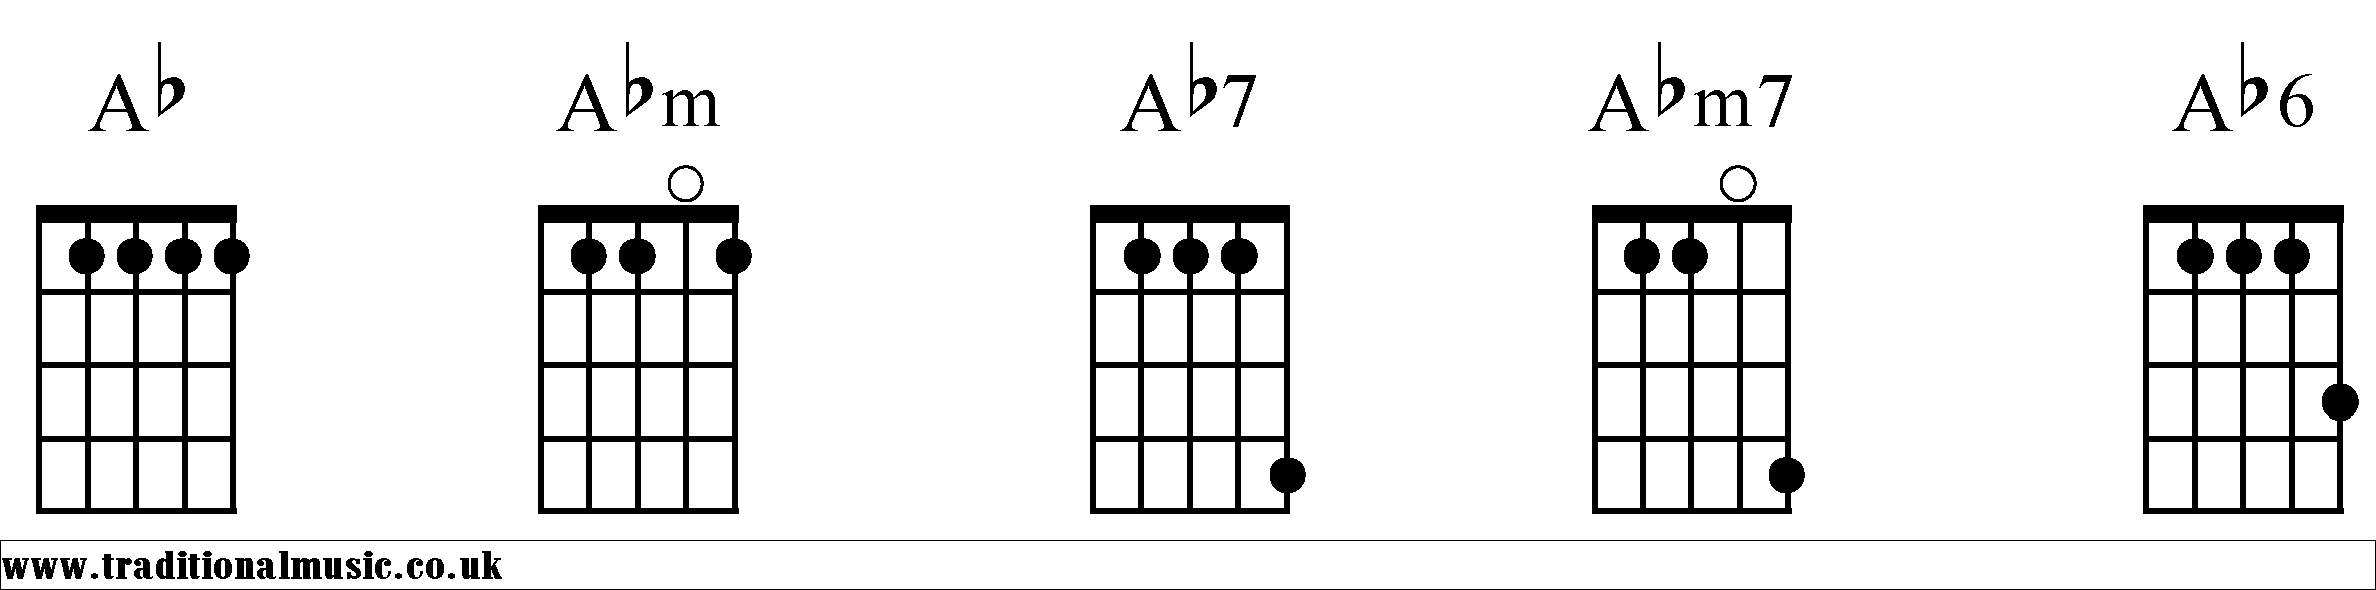
\includegraphics[scale=.15]{chords/Abbjo1}
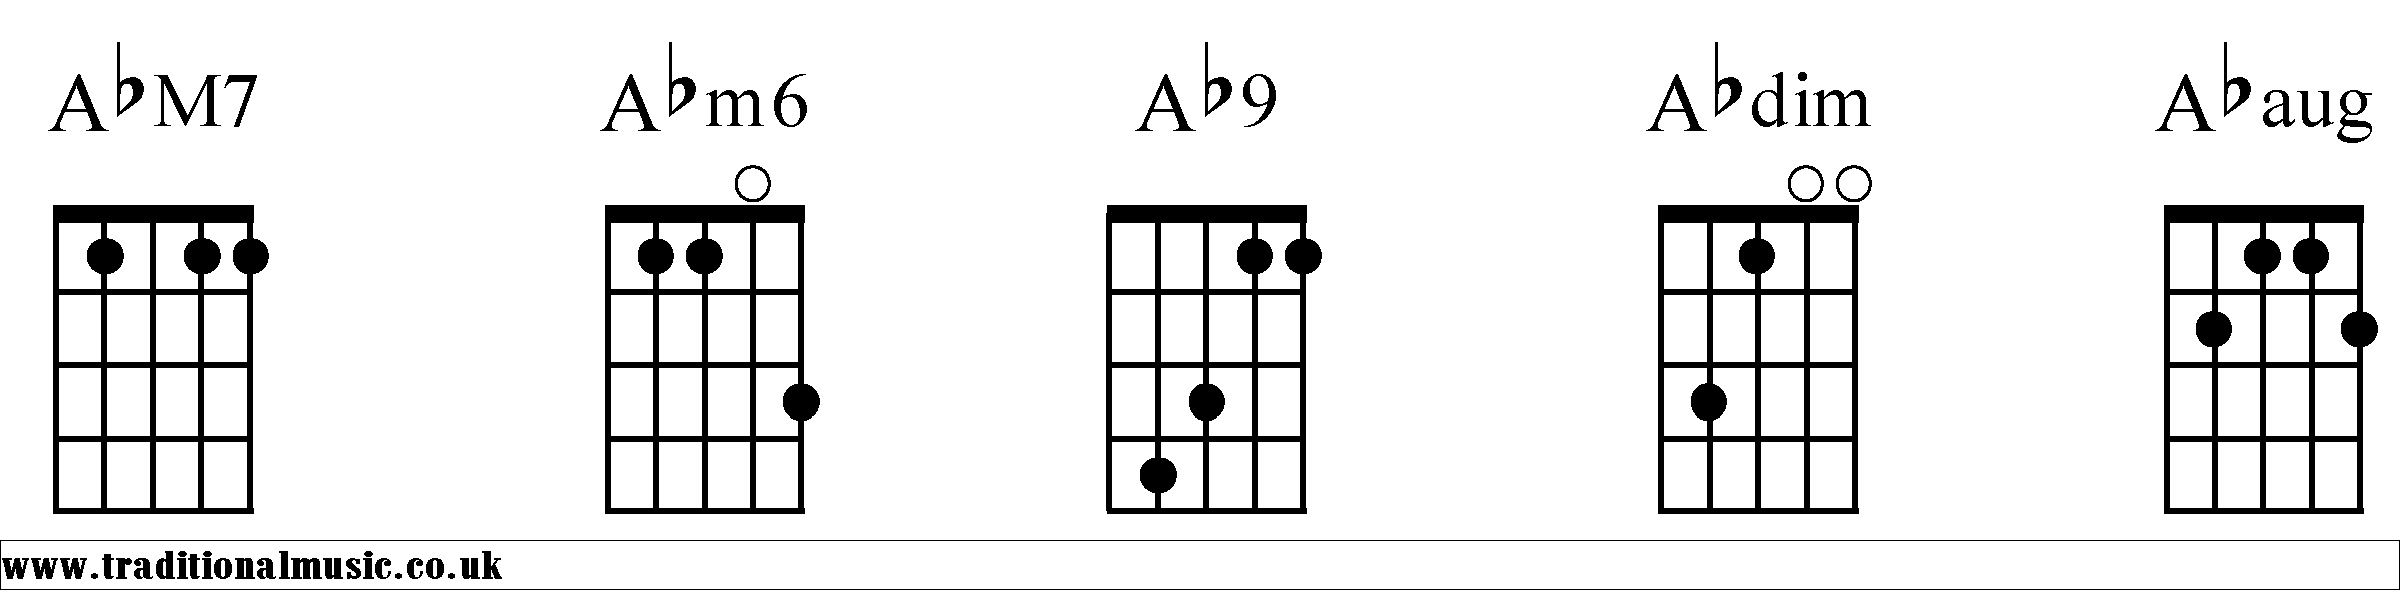
\includegraphics[scale=.15]{chords/Abbjo2}

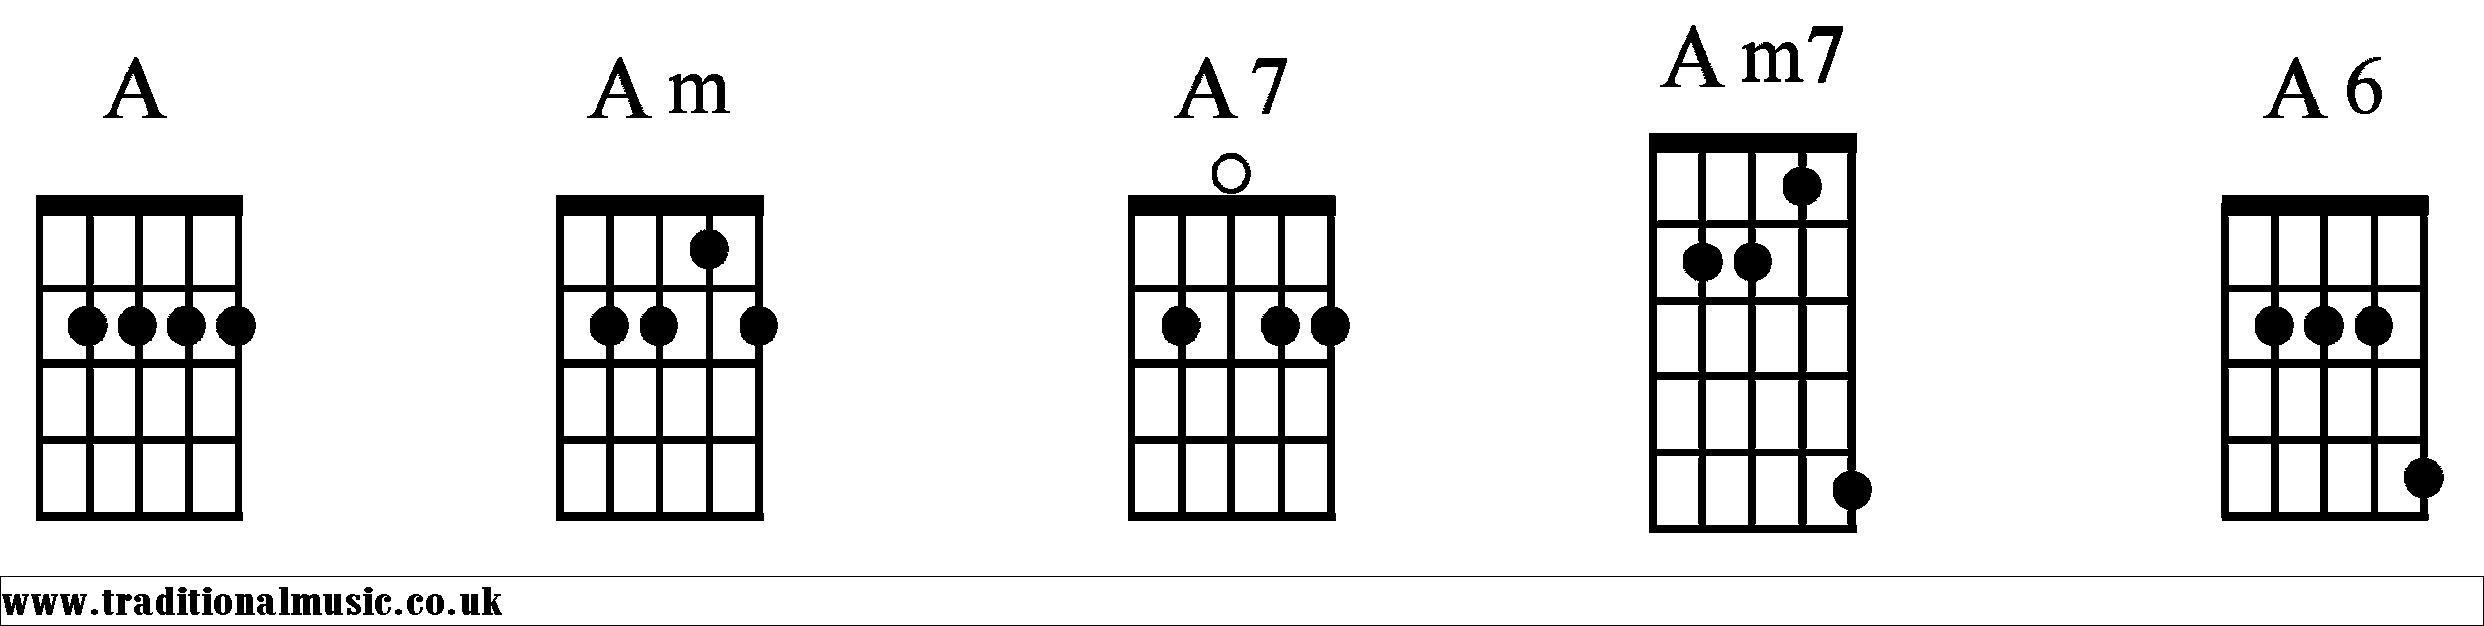
\includegraphics[scale=.15]{chords/Abjo1}
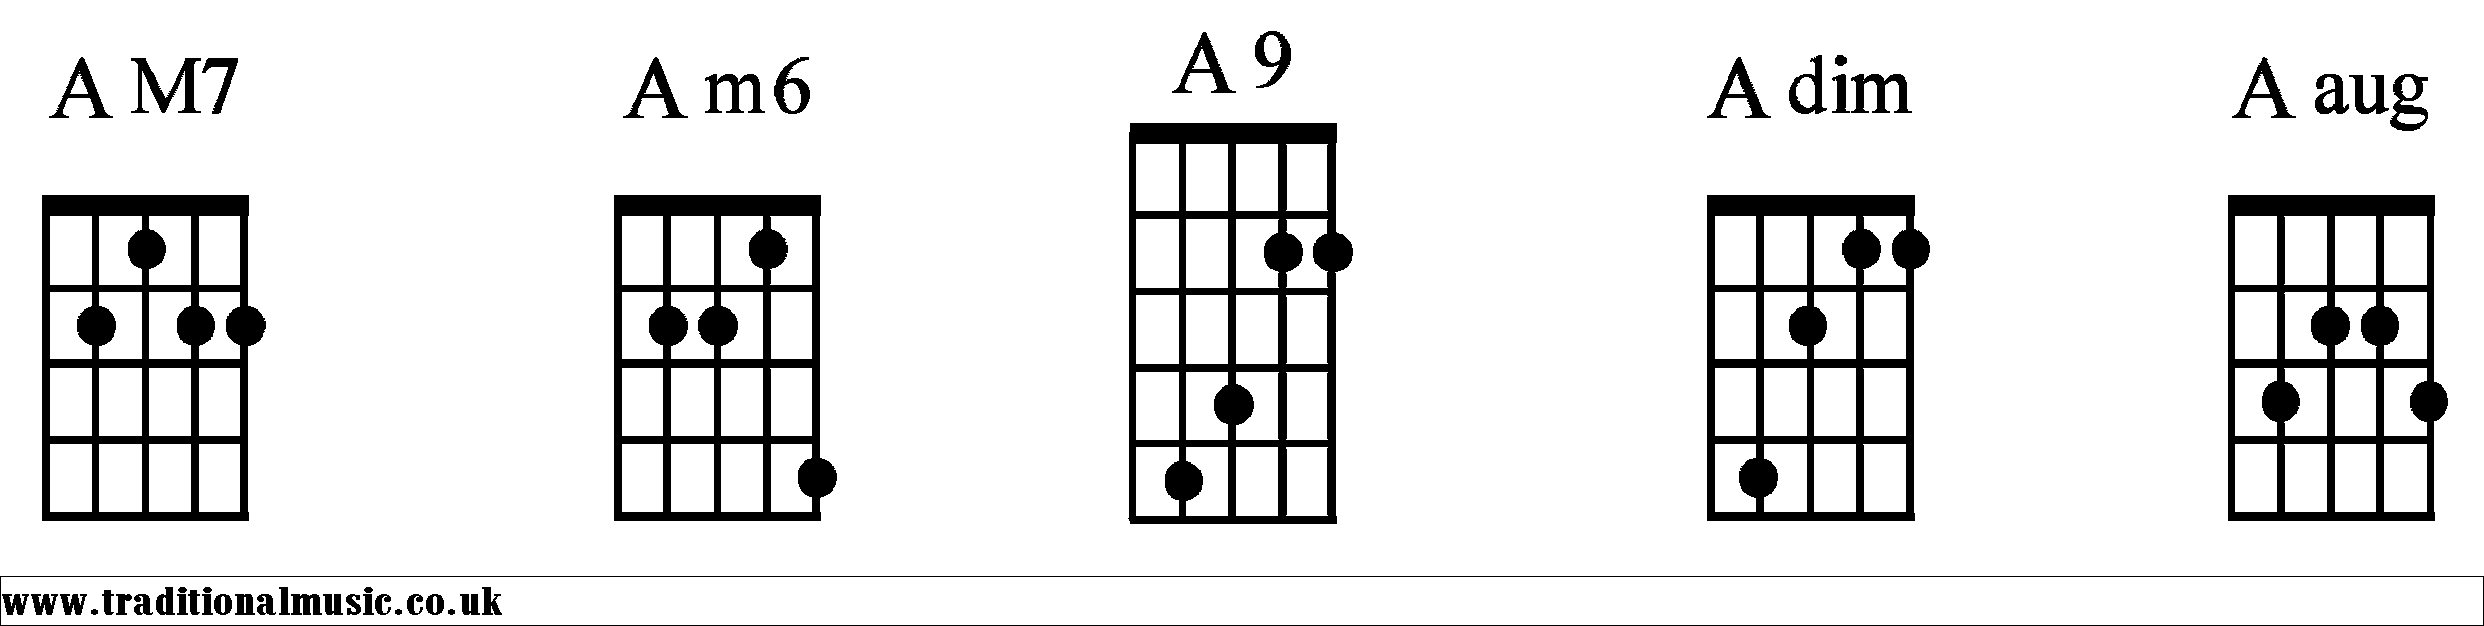
\includegraphics[scale=.15]{chords/Abjo2}

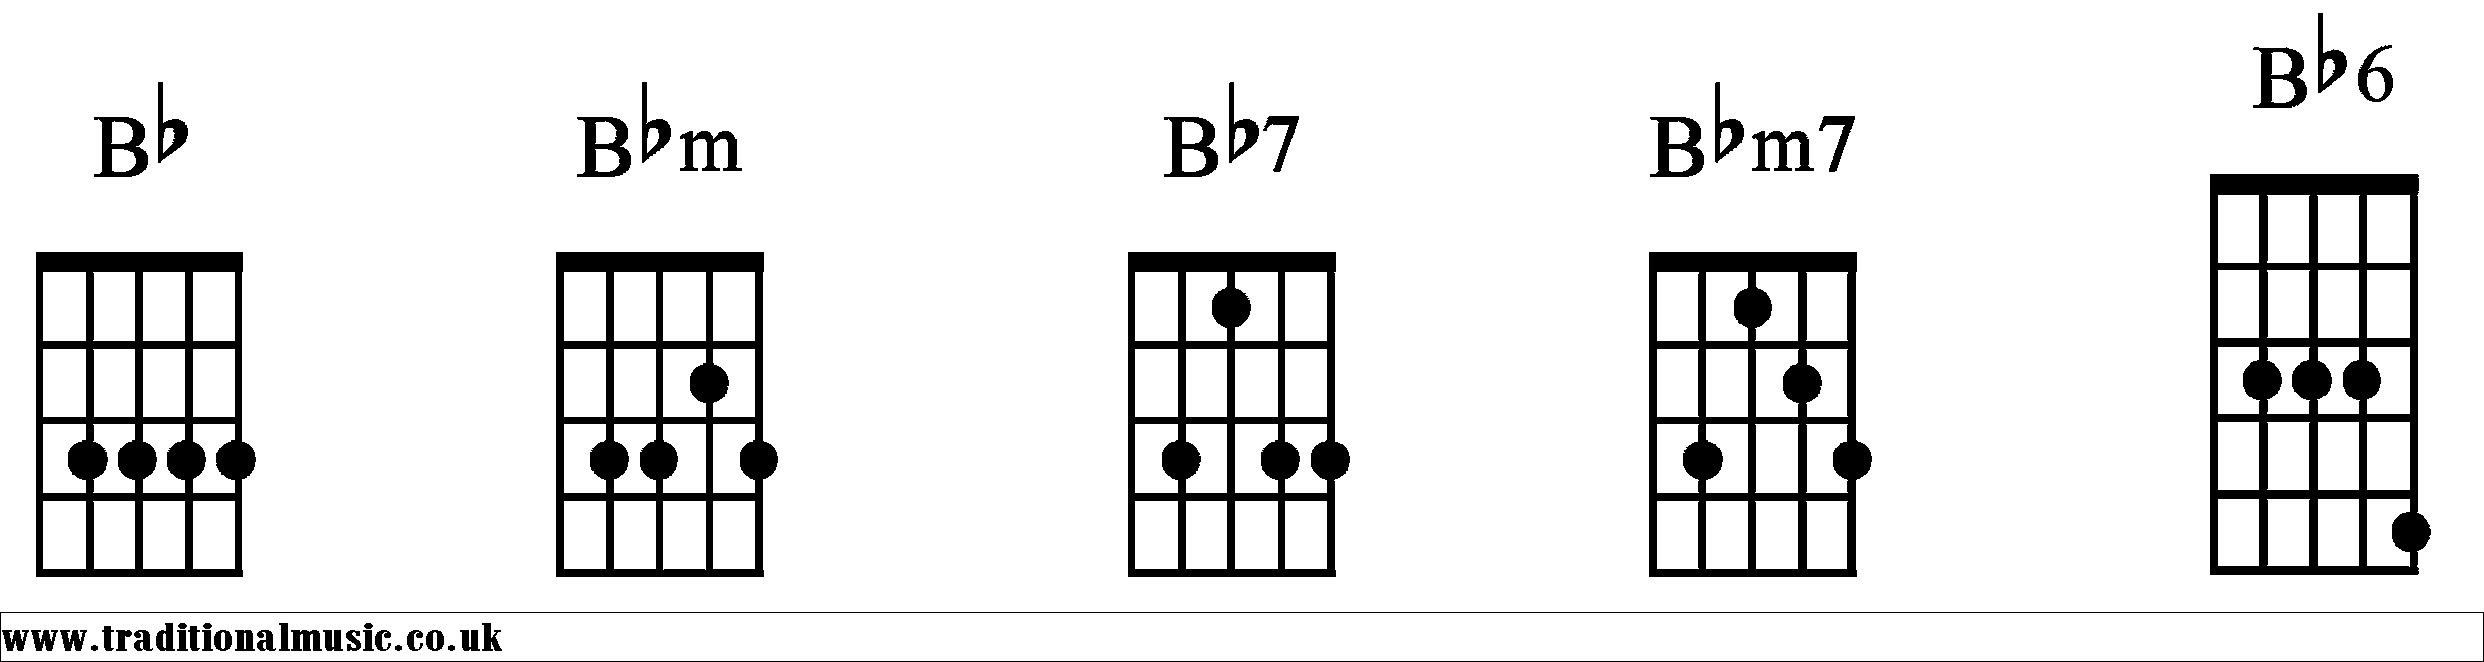
\includegraphics[scale=.15]{chords/Bbbjo1}
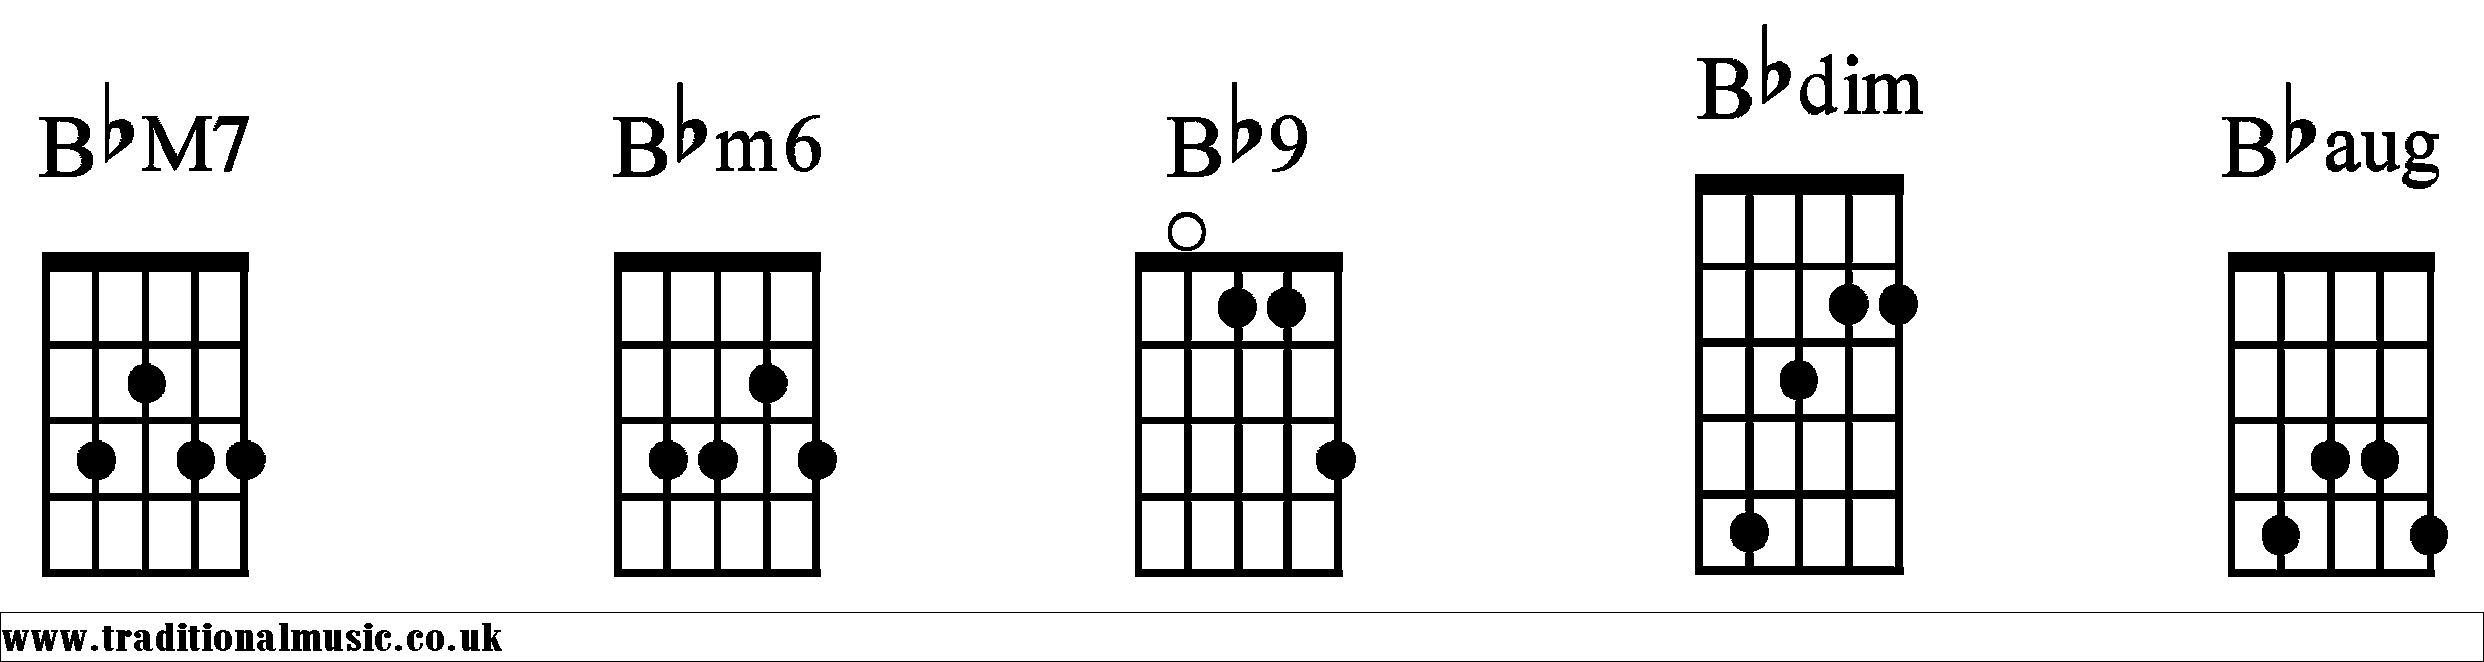
\includegraphics[scale=.15]{chords/Bbbjo2}

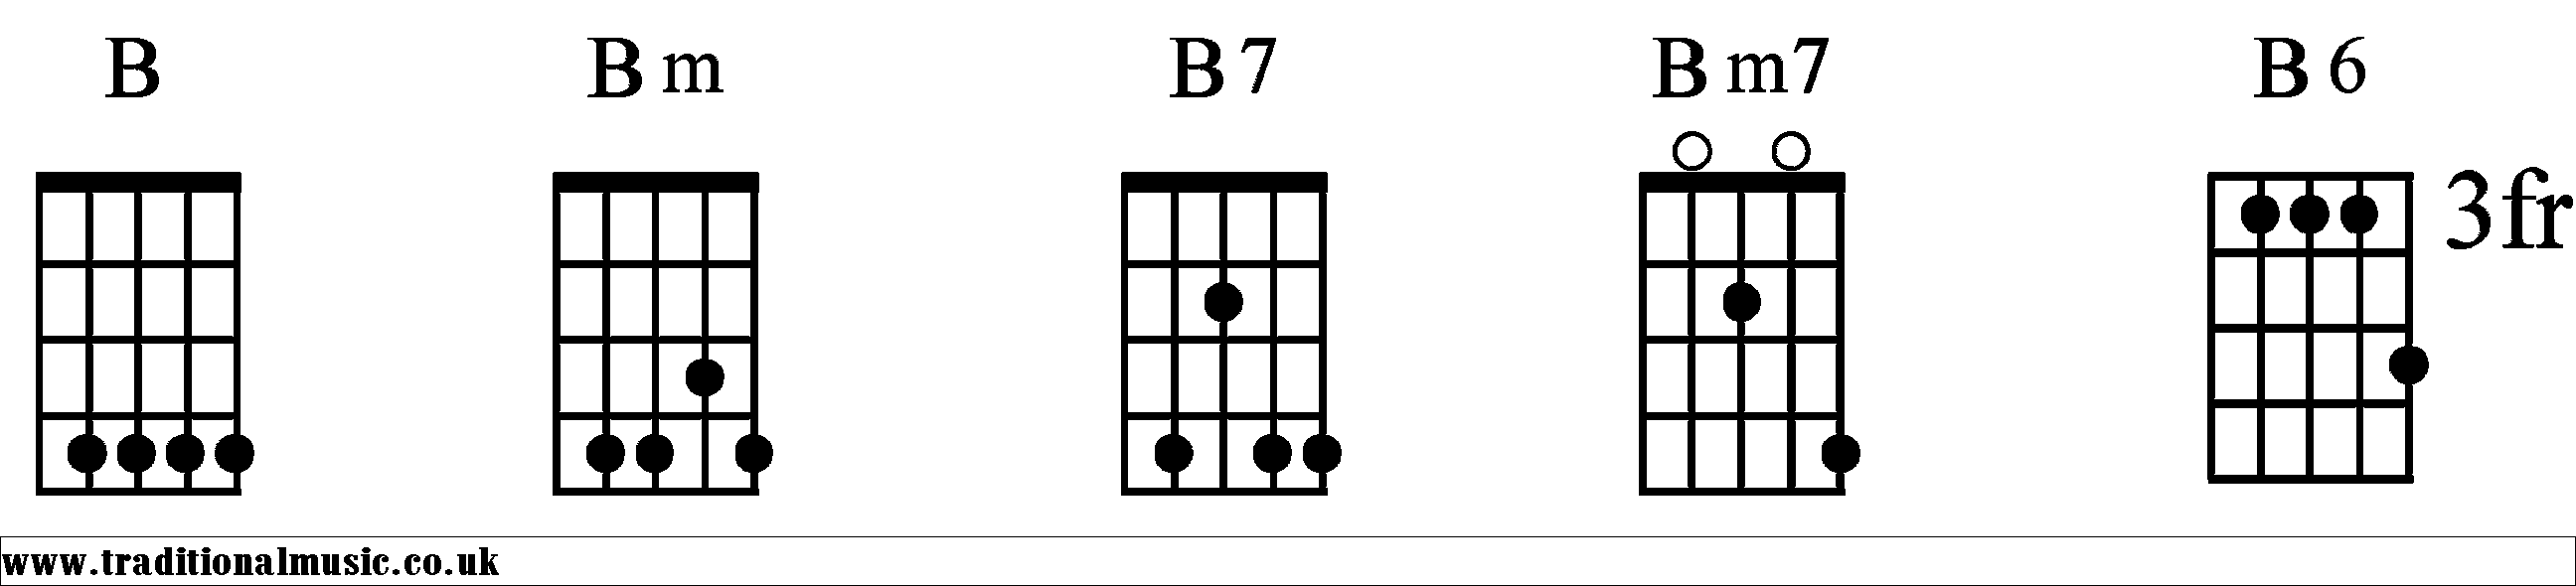
\includegraphics[scale=.15]{chords/Bbjo1}
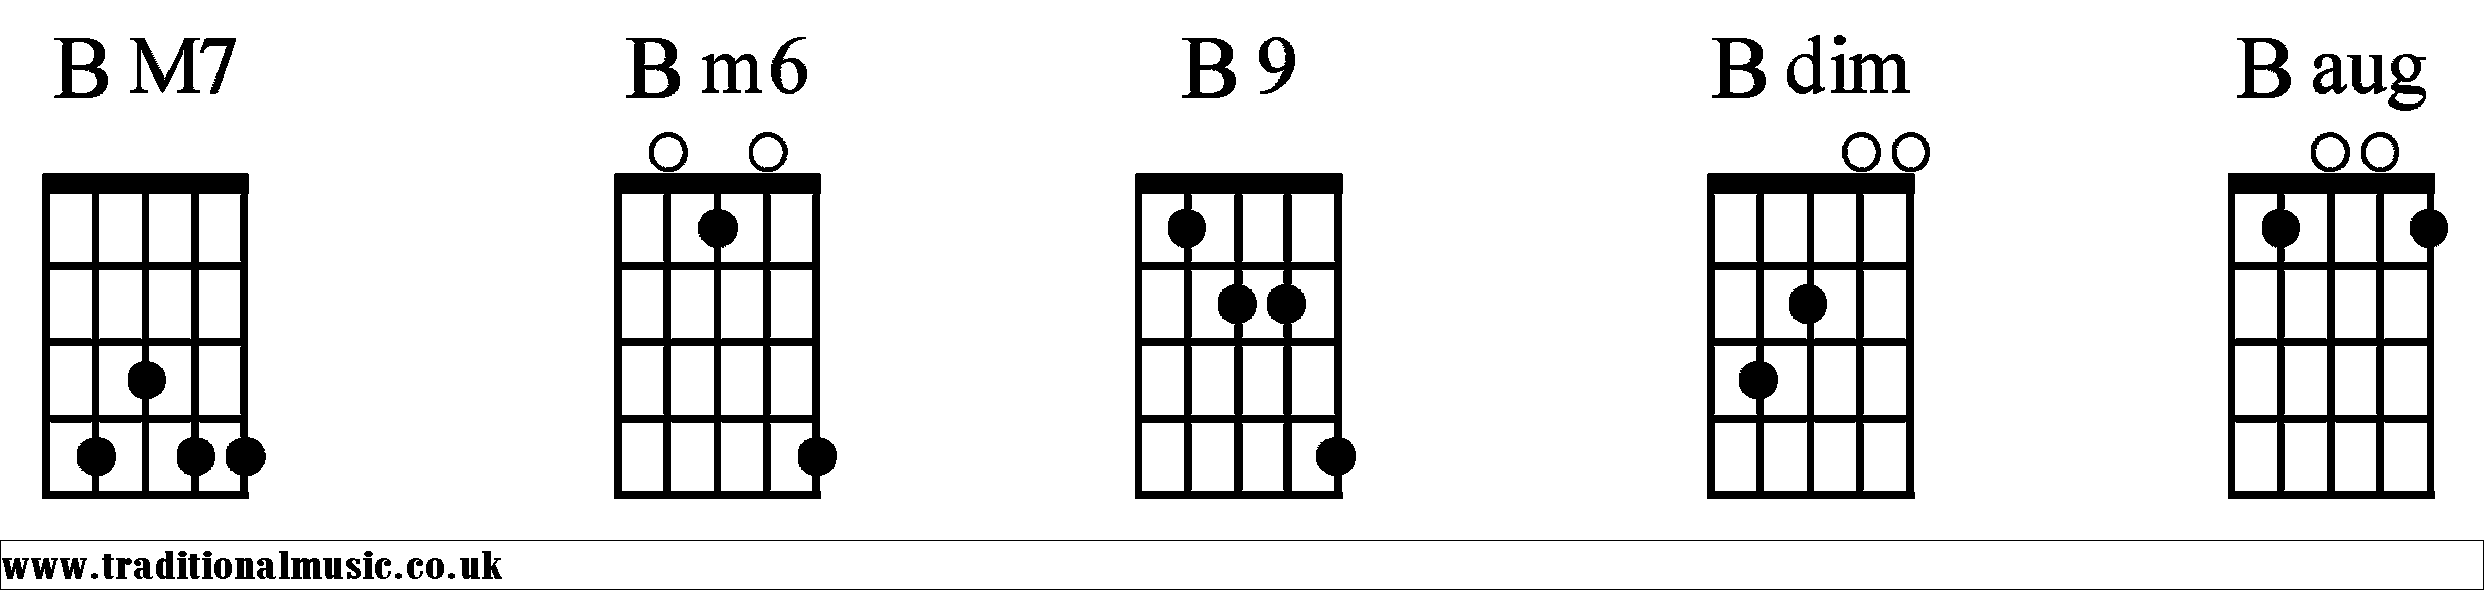
\includegraphics[scale=.15]{chords/Bbjo2}

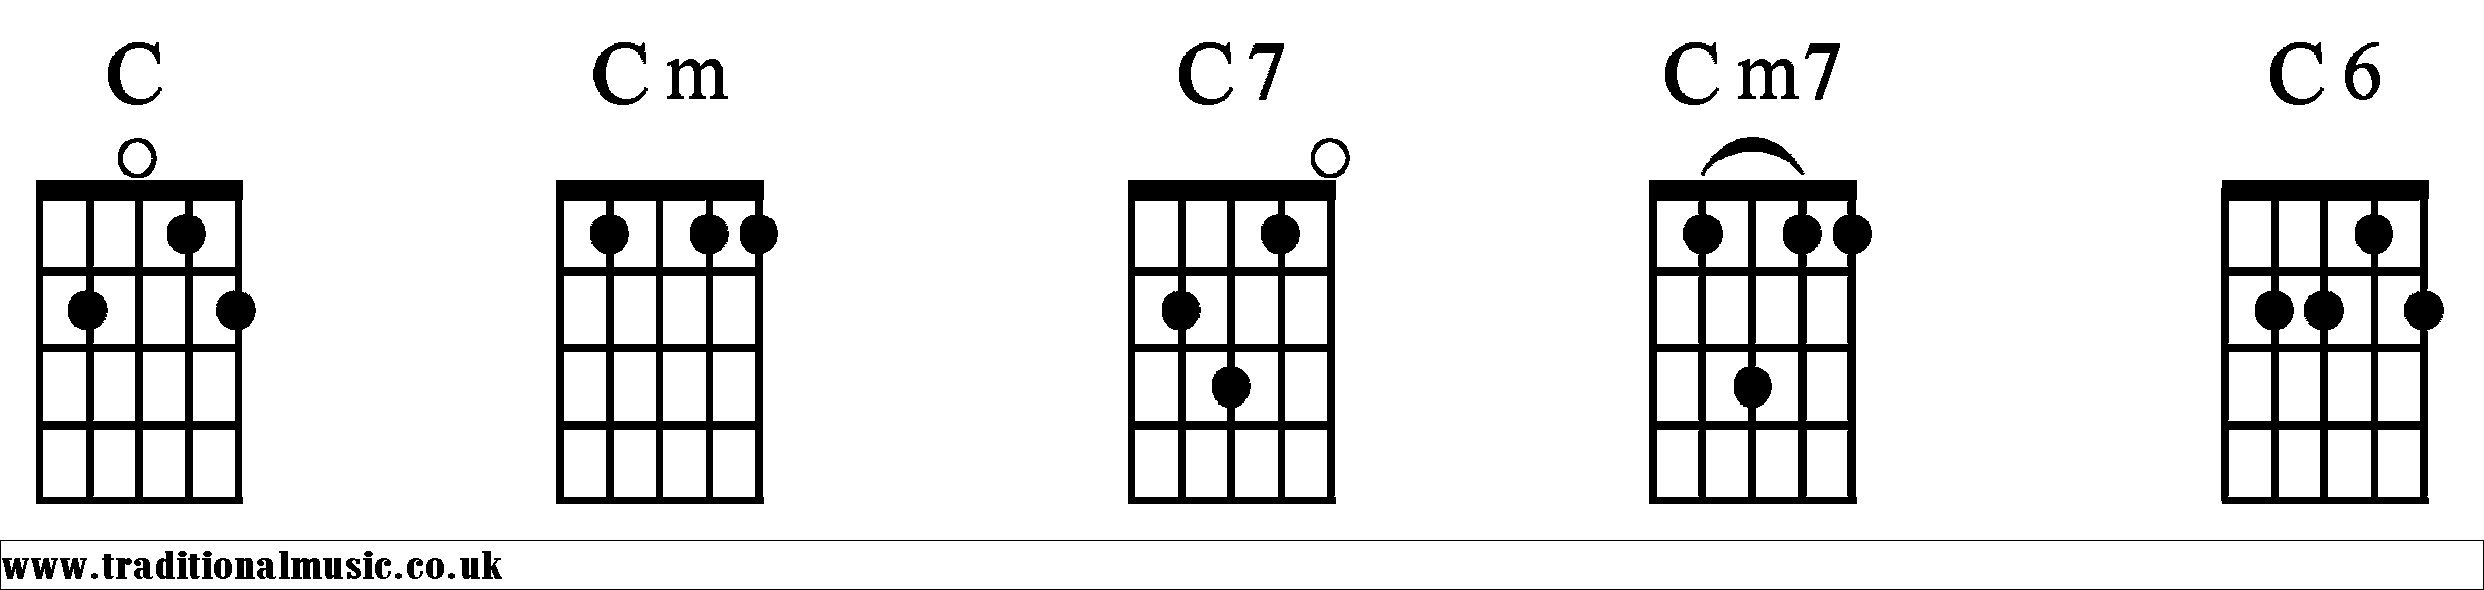
\includegraphics[scale=.15]{chords/Cbjo1}
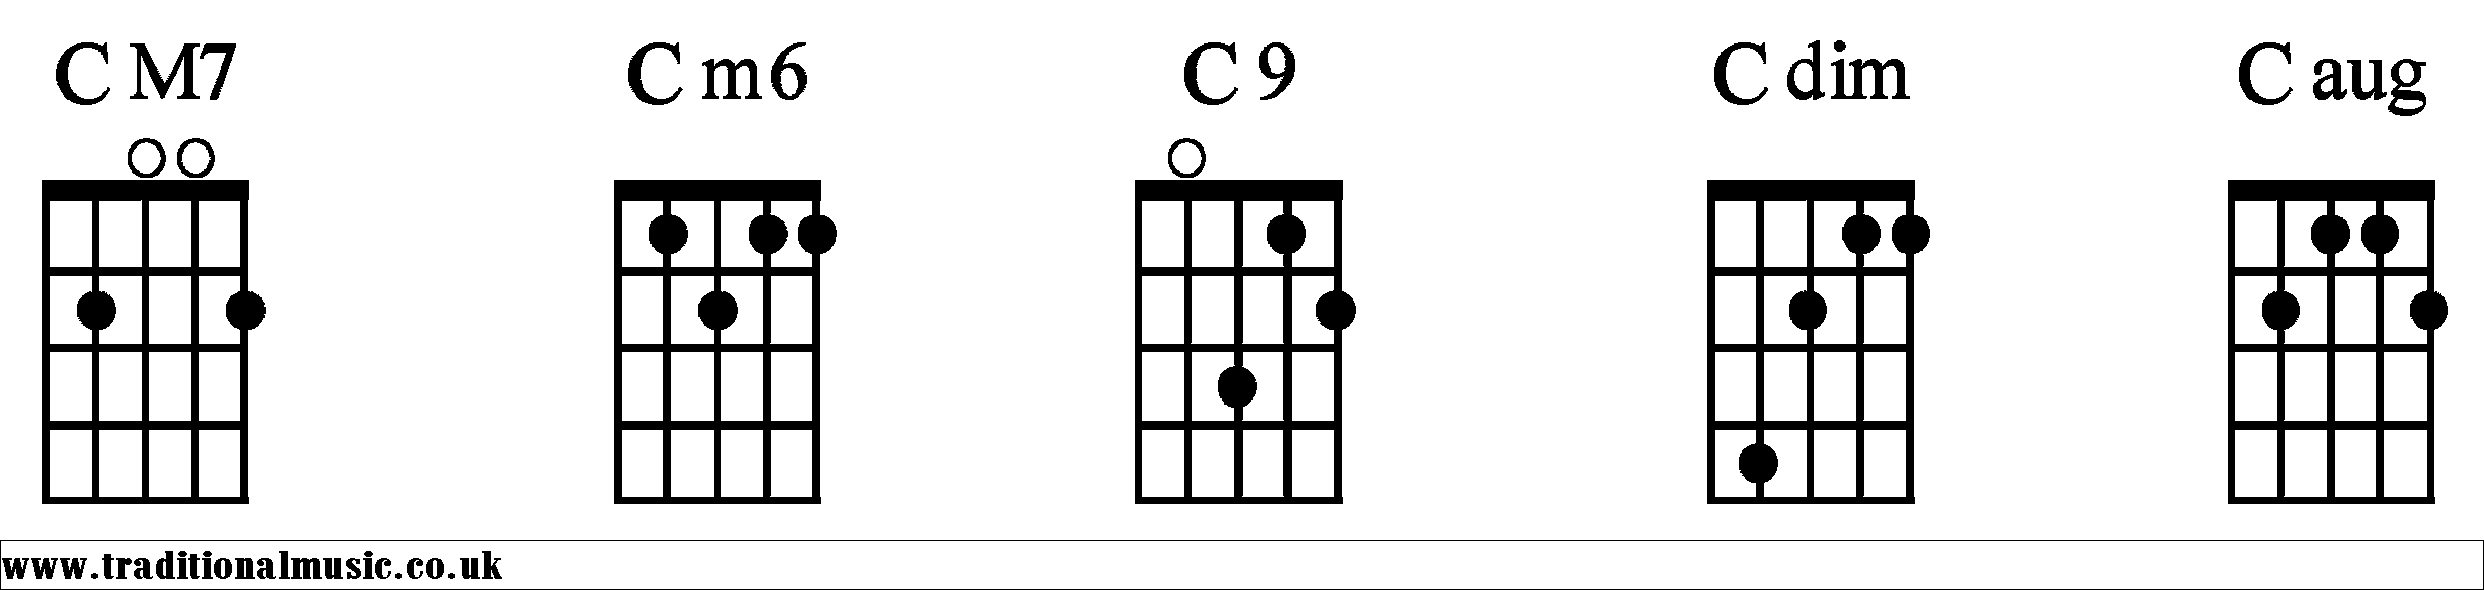
\includegraphics[scale=.15]{chords/Cbjo2}

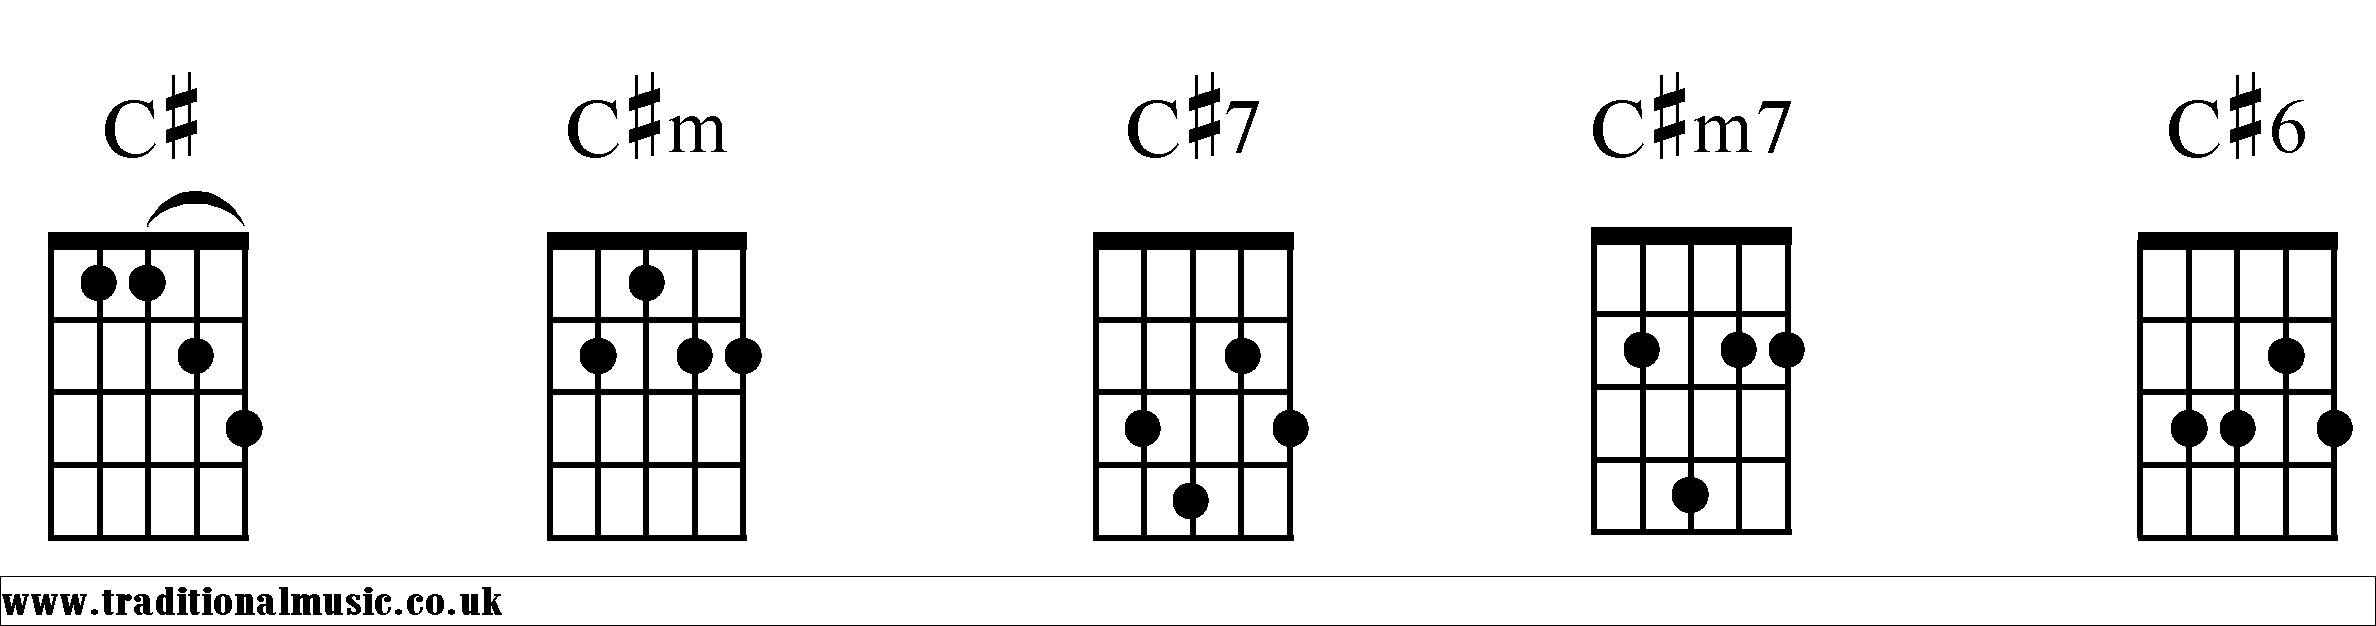
\includegraphics[scale=.15]{chords/Csbjo1}
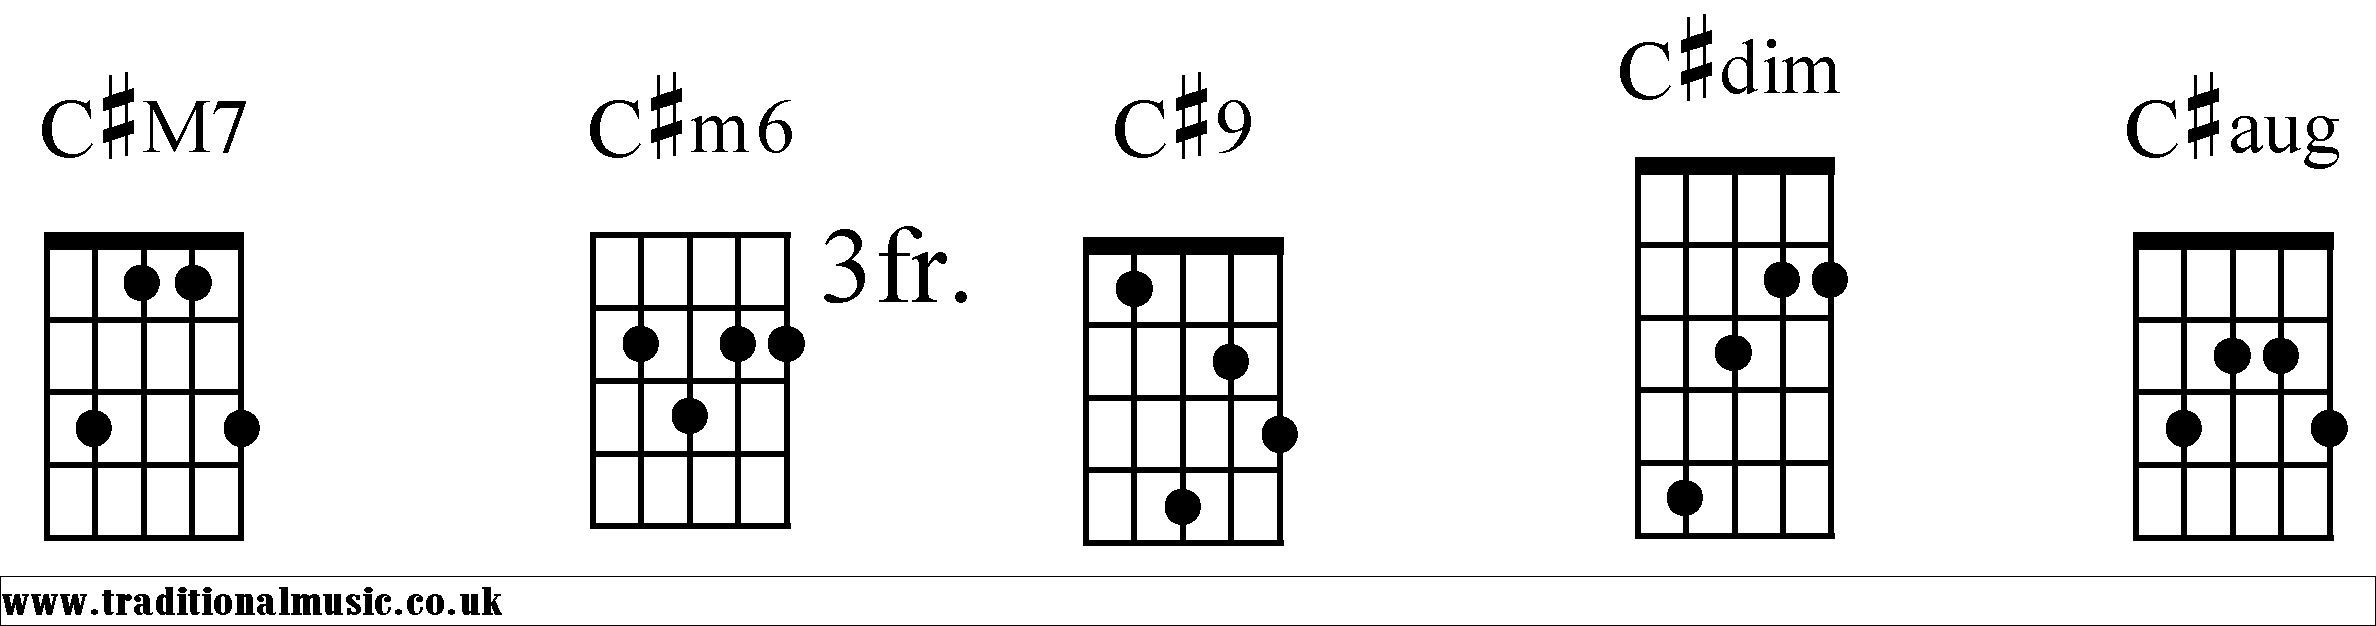
\includegraphics[scale=.15]{chords/Csbjo2}

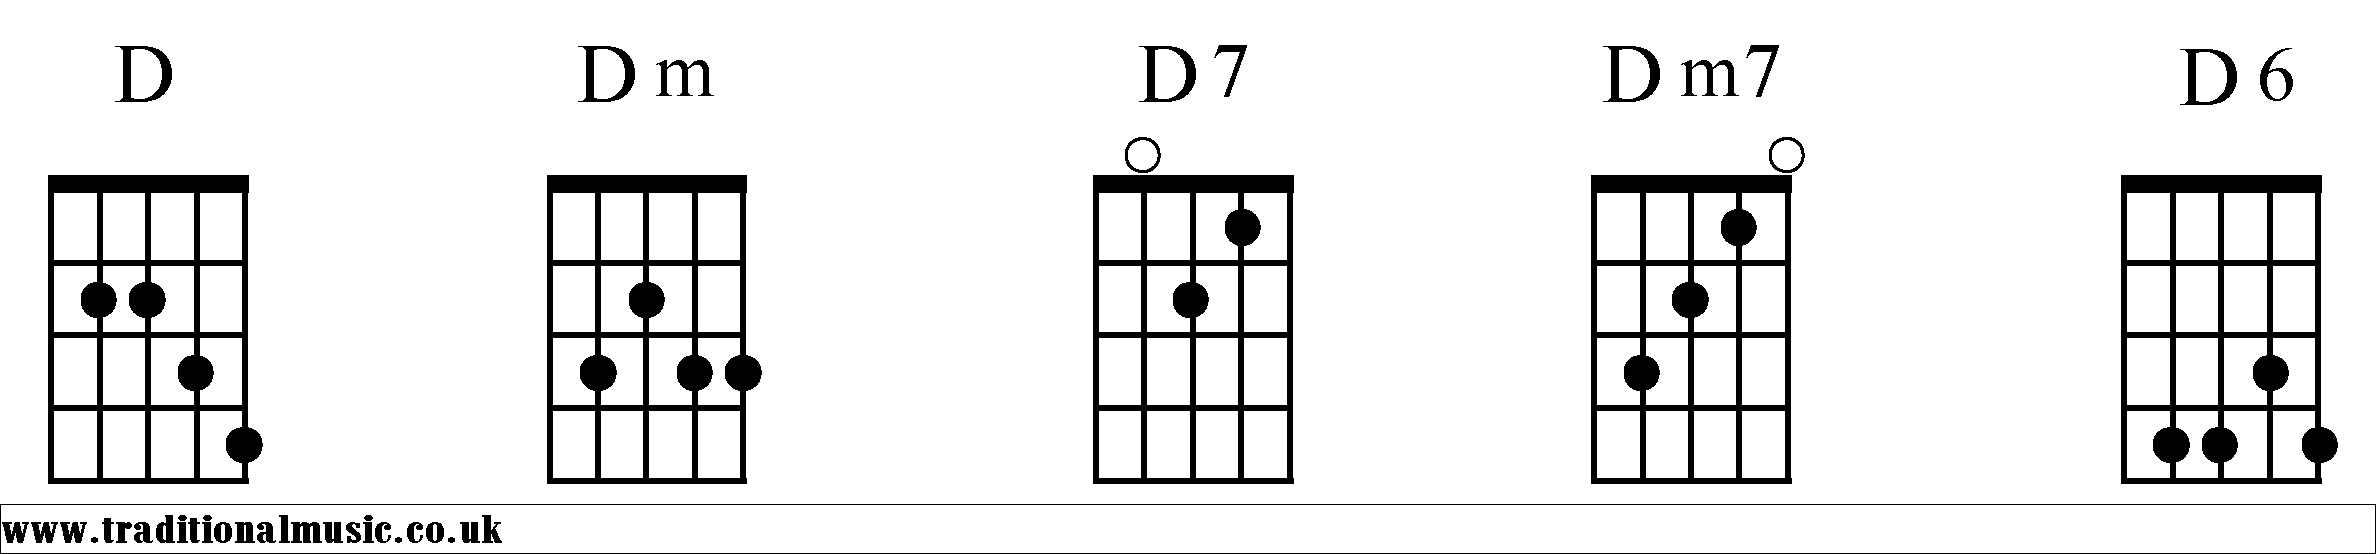
\includegraphics[scale=.15]{chords/Dbjo1}
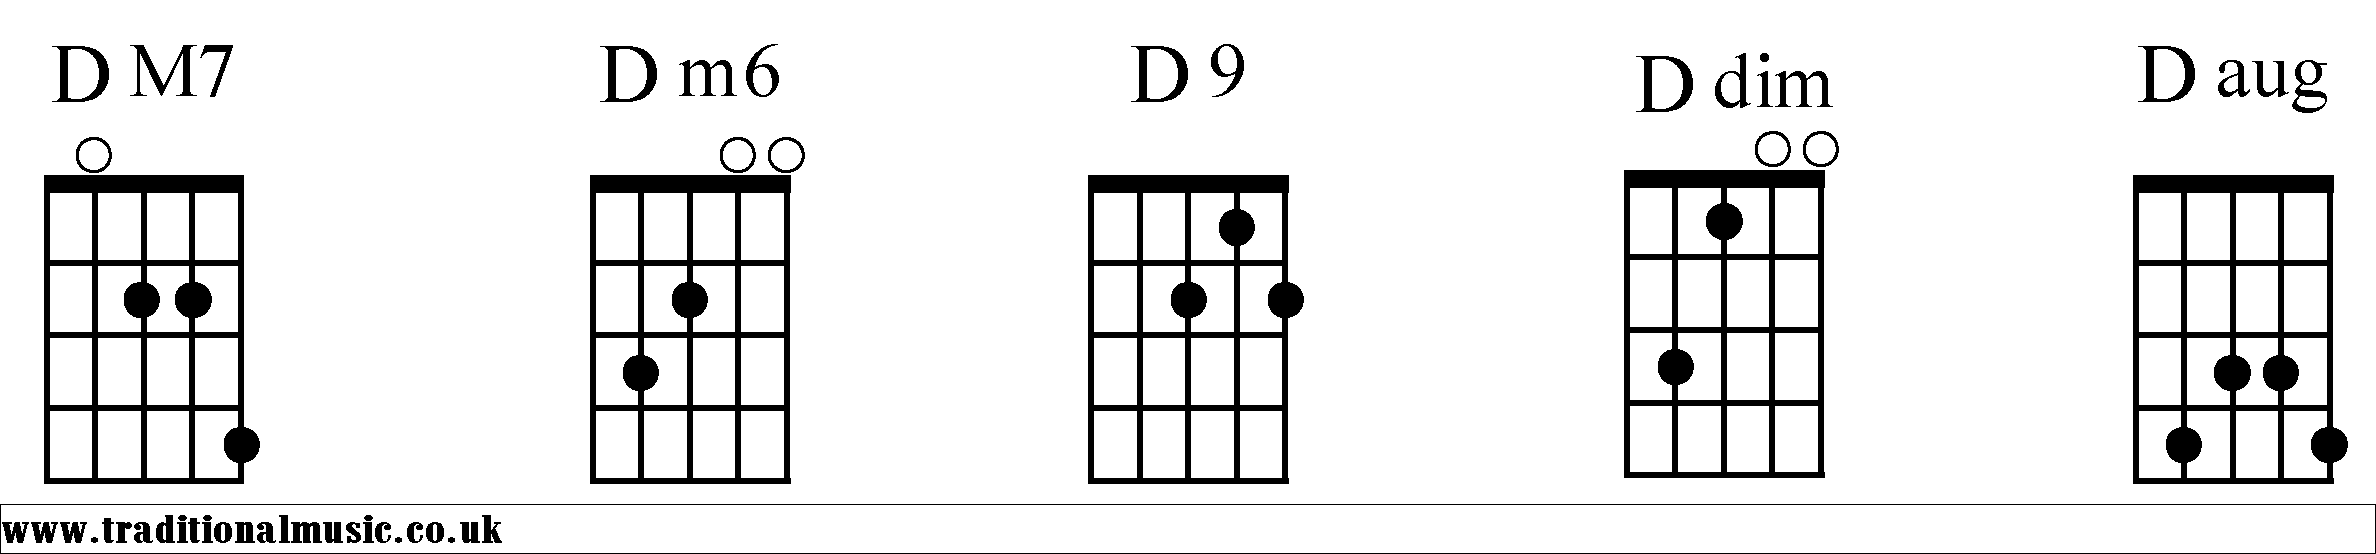
\includegraphics[scale=.15]{chords/Dbjo2}

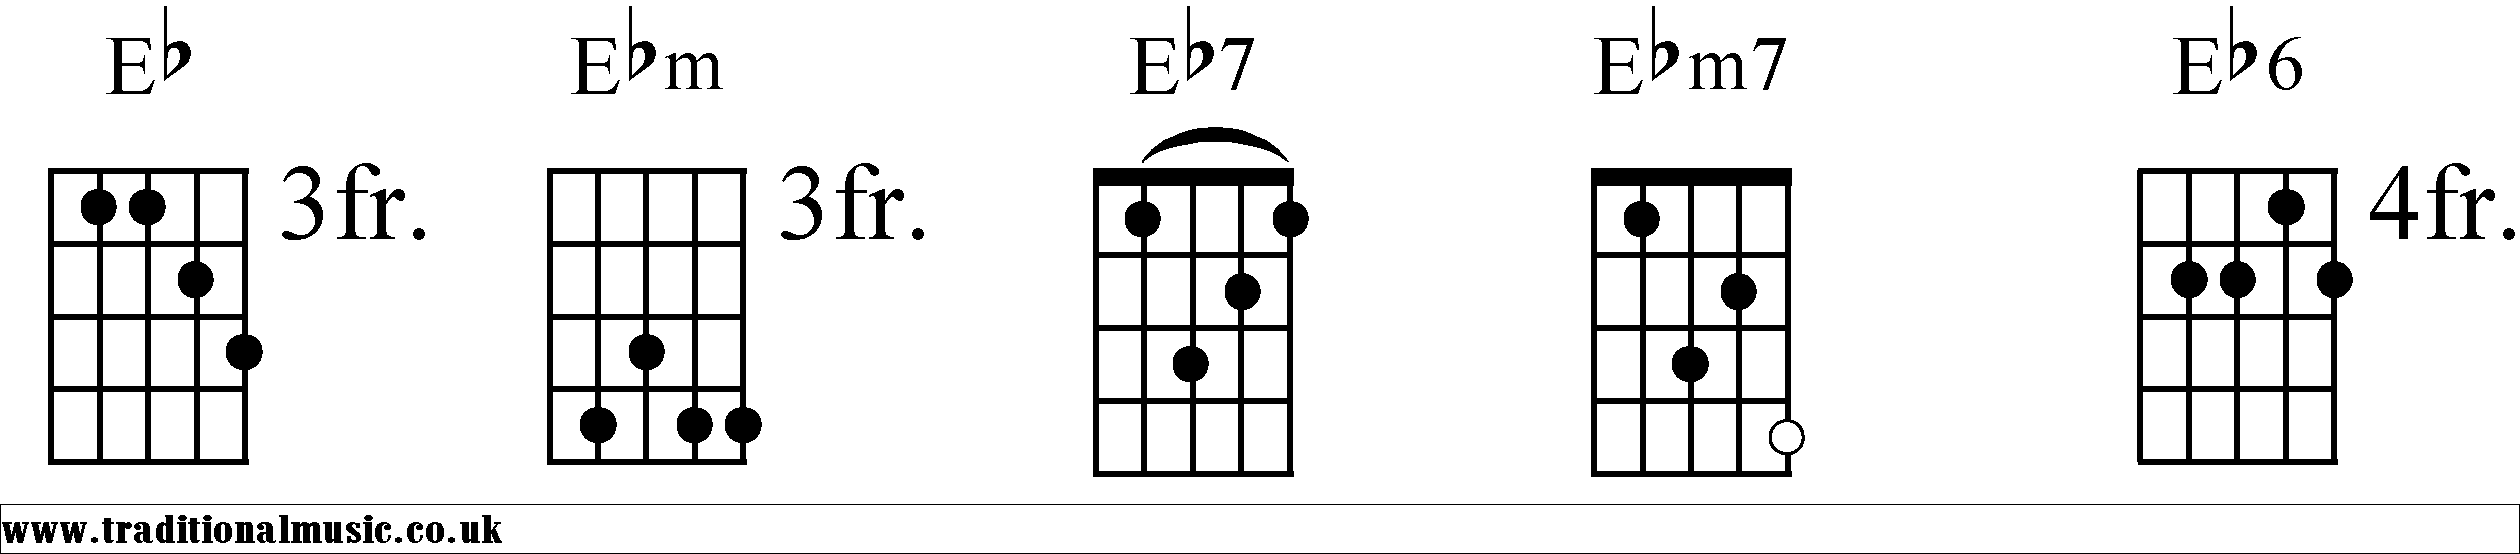
\includegraphics[scale=.15]{chords/Ebbjo1}
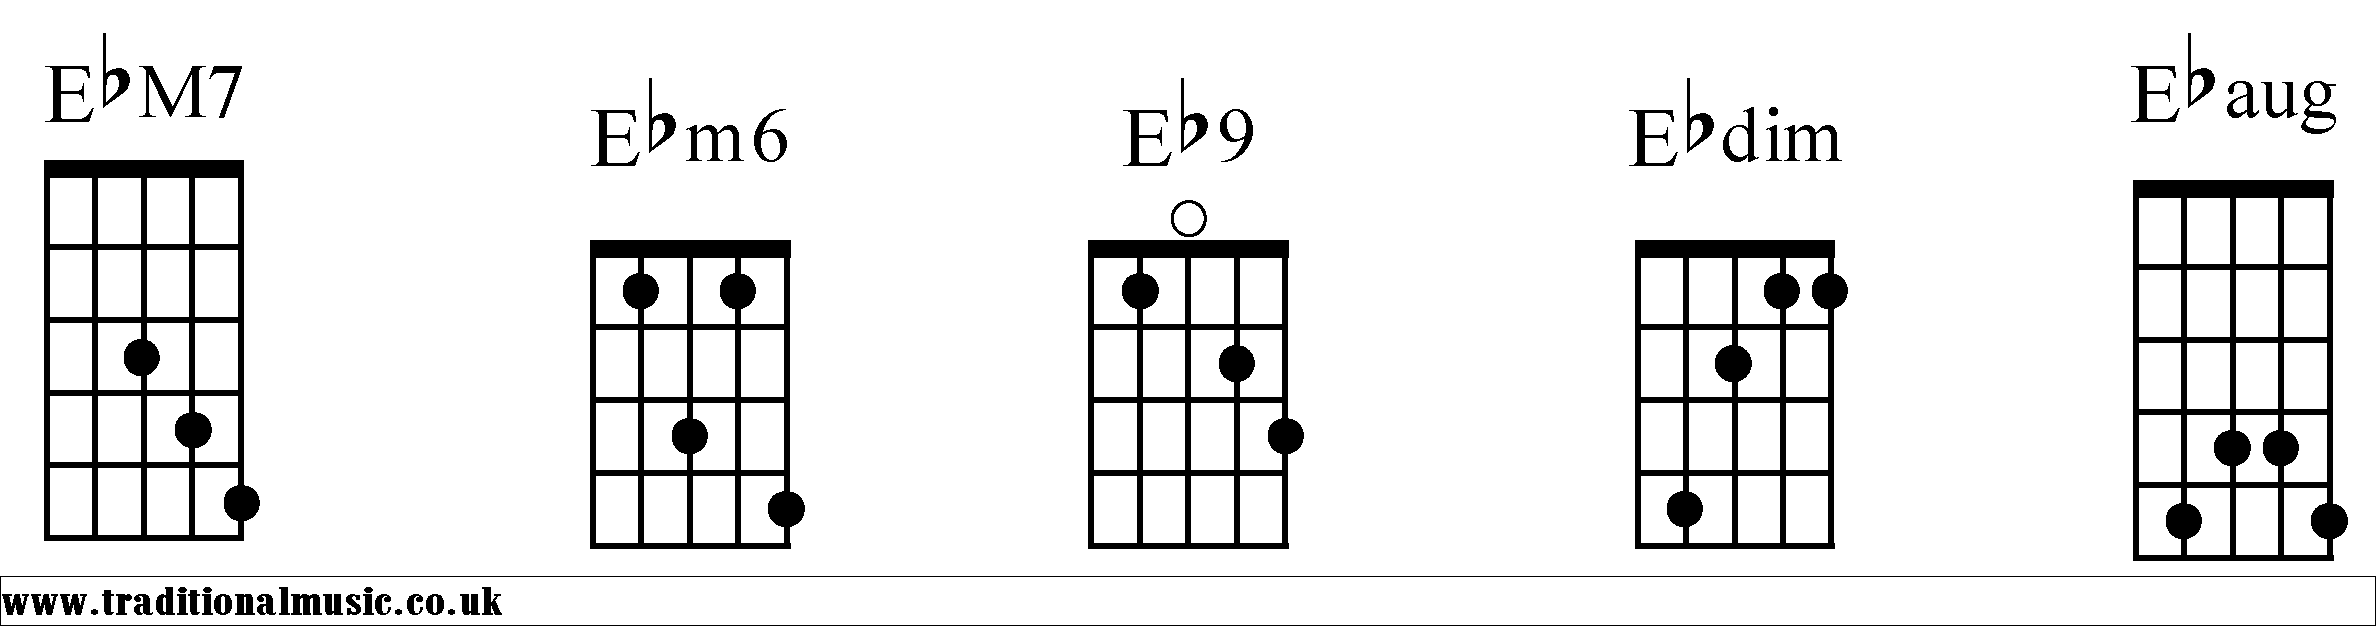
\includegraphics[scale=.15]{chords/Ebbjo2}

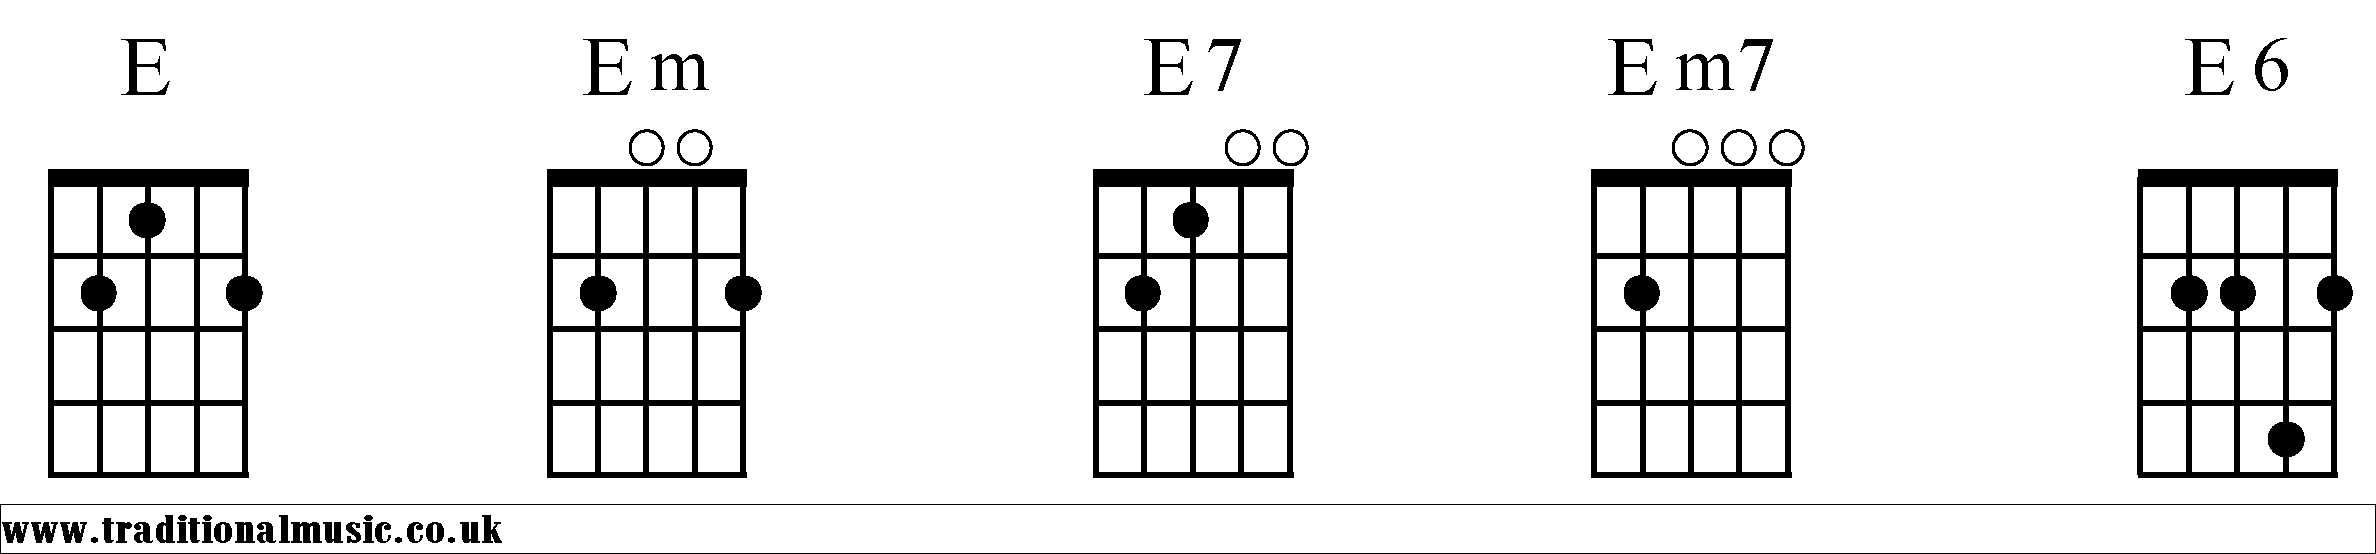
\includegraphics[scale=.15]{chords/Ebjo1}
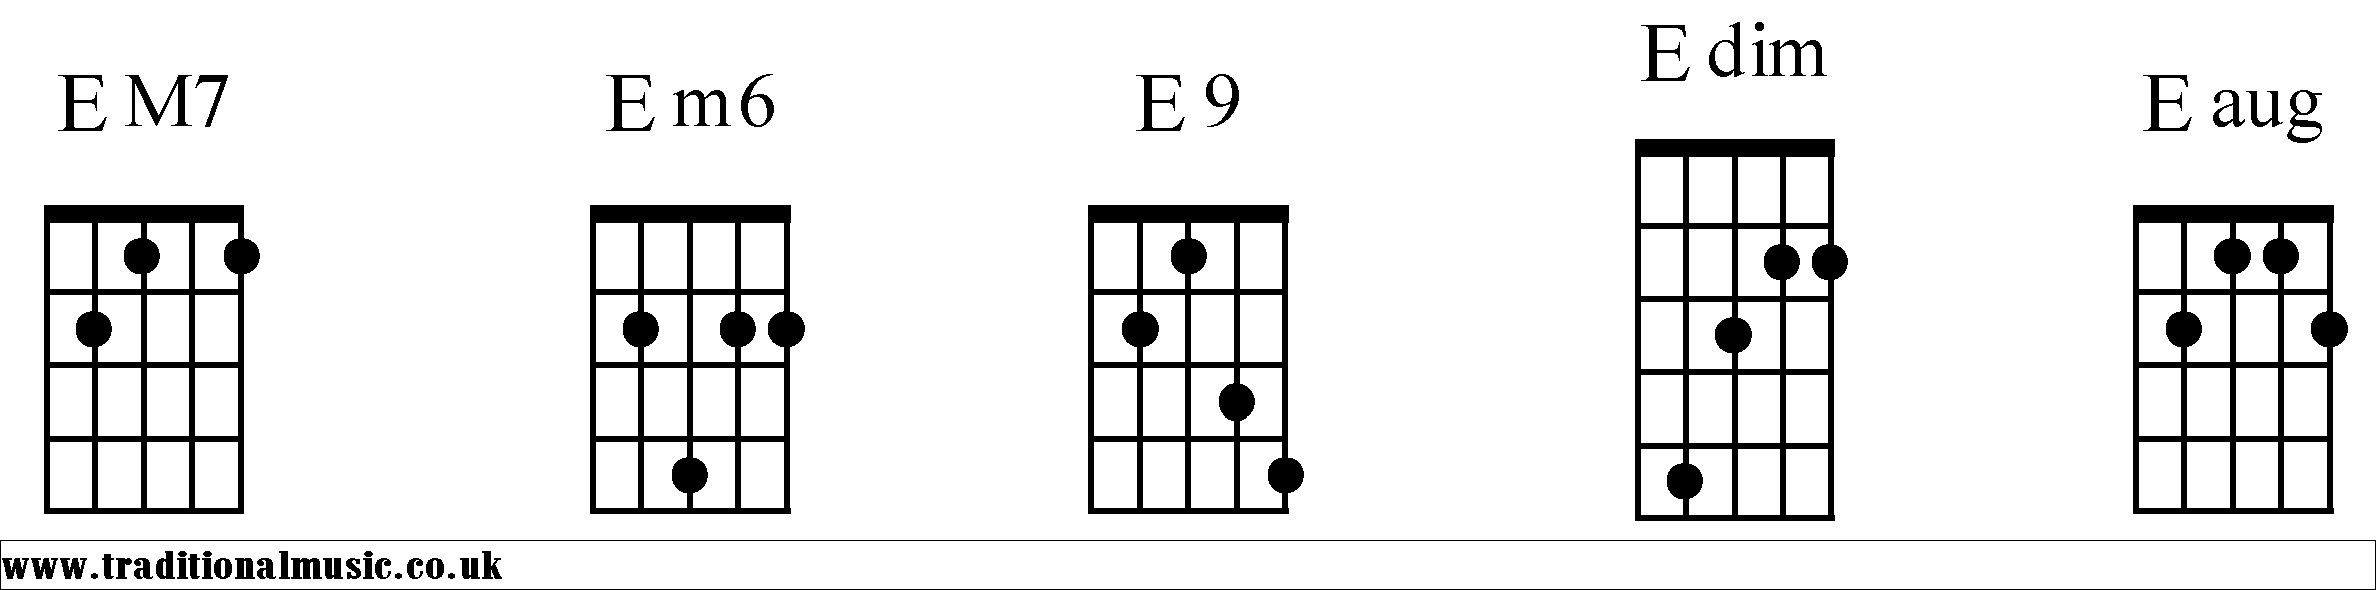
\includegraphics[scale=.15]{chords/Ebjo2}

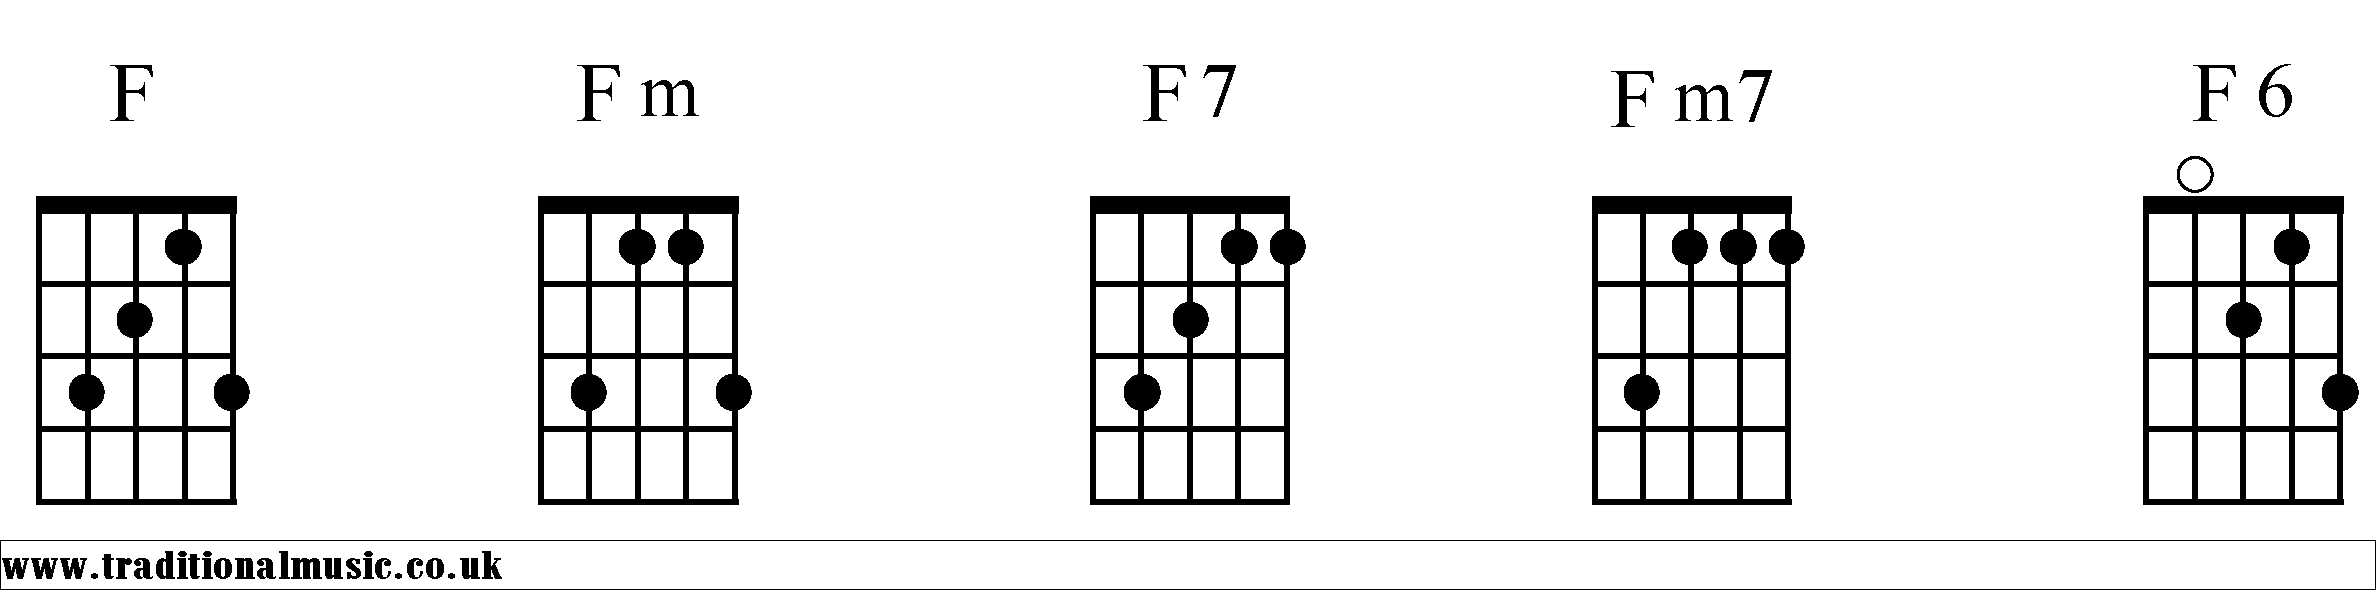
\includegraphics[scale=.15]{chords/Fbjo1}
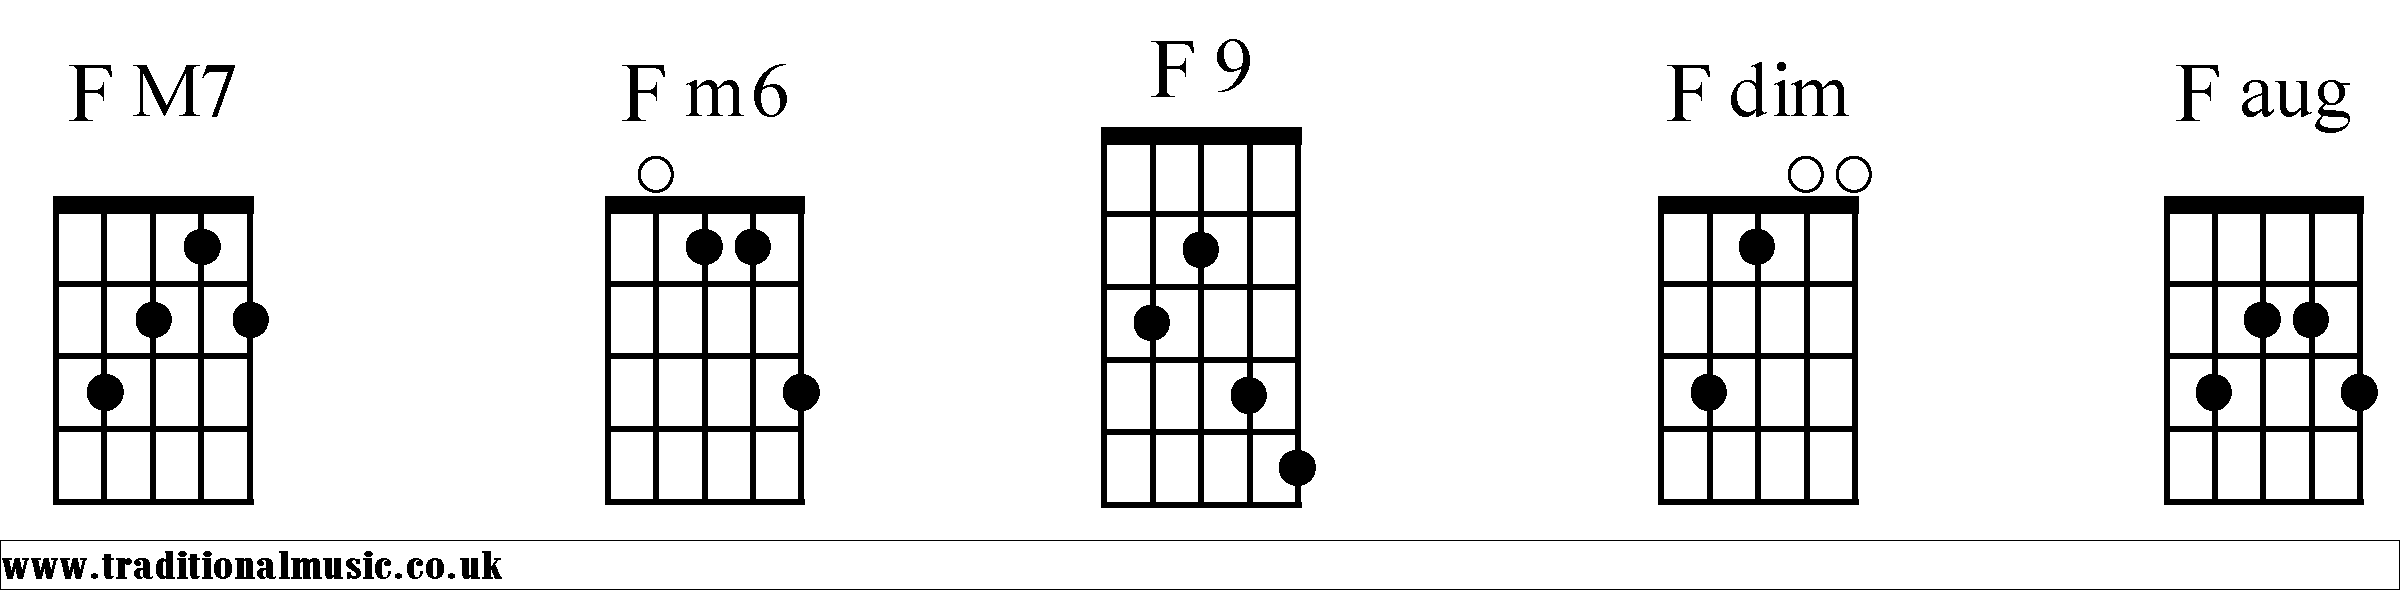
\includegraphics[scale=.15]{chords/Fbjo2}

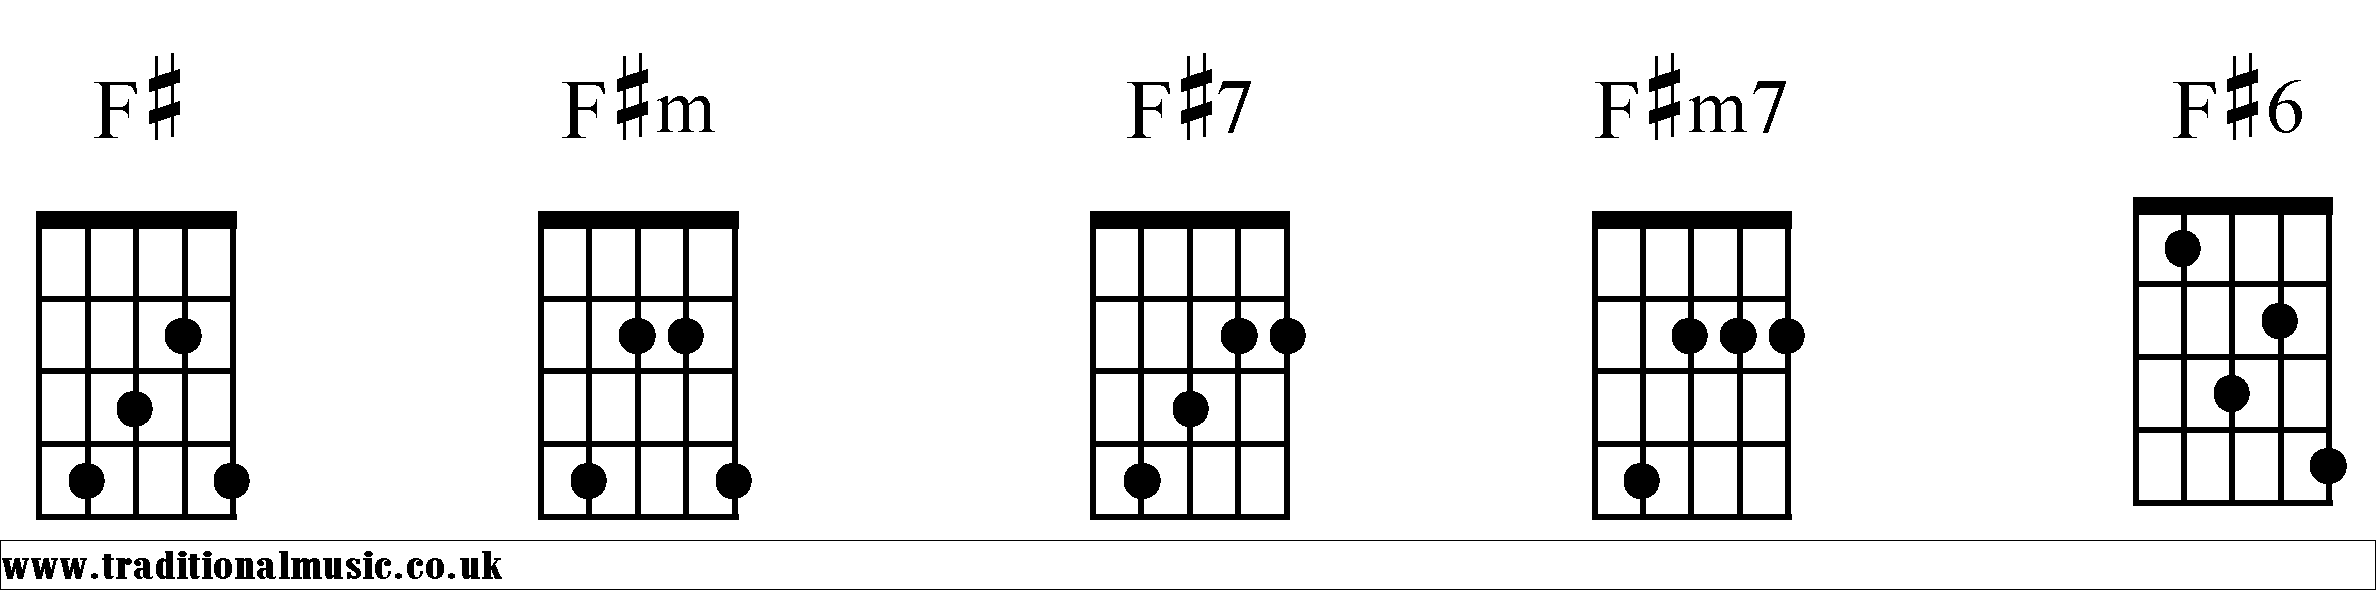
\includegraphics[scale=.15]{chords/Fsbjo1}
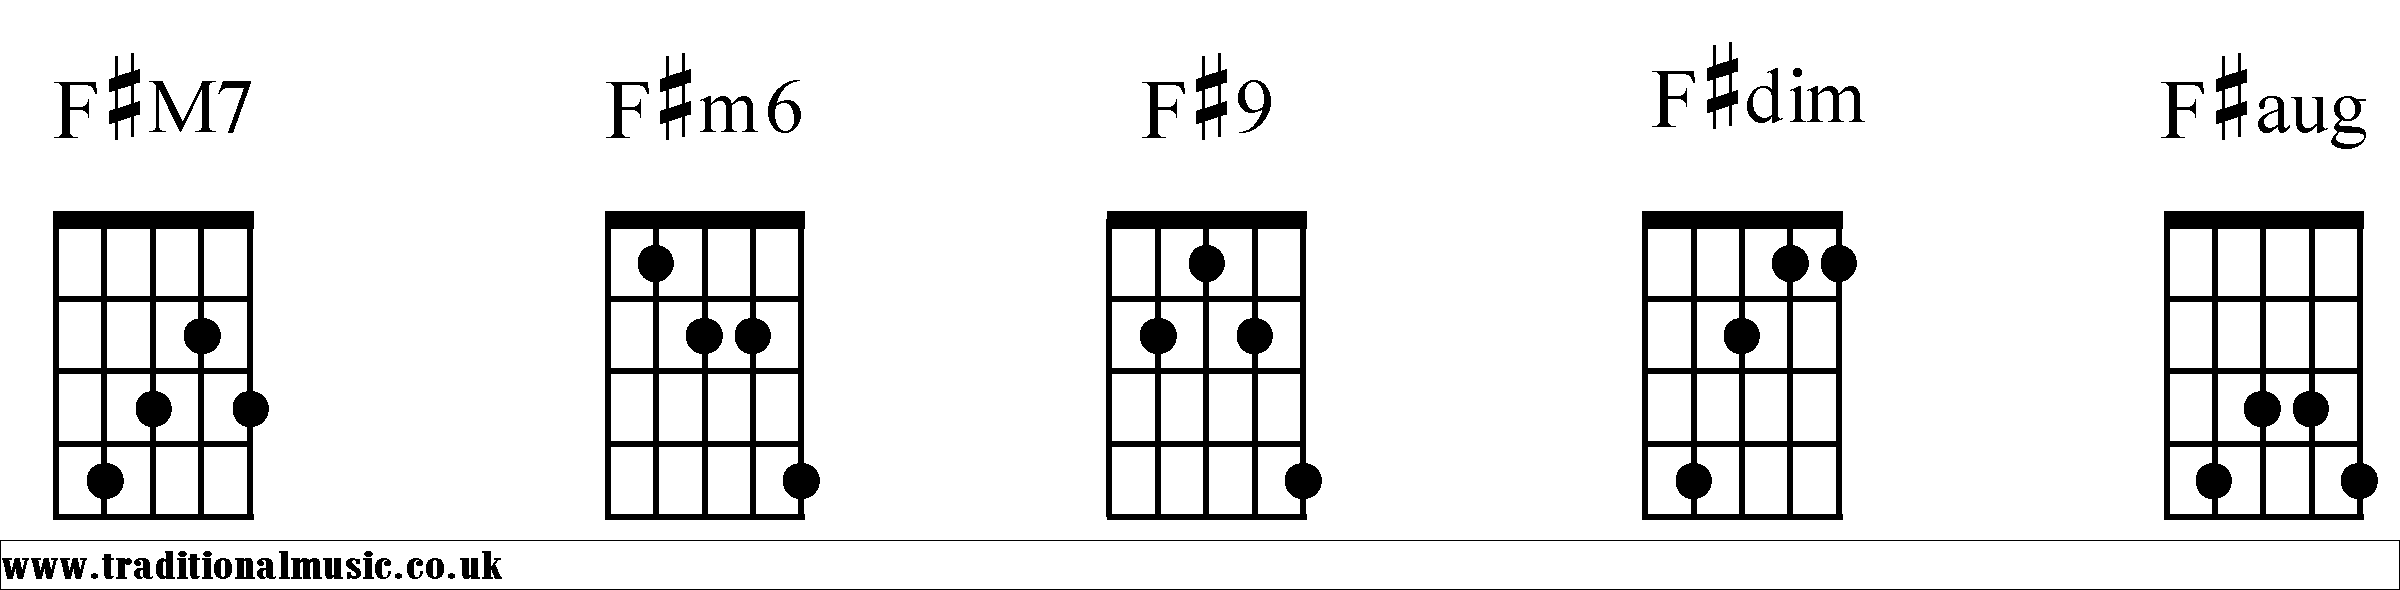
\includegraphics[scale=.15]{chords/Fsbjo2}

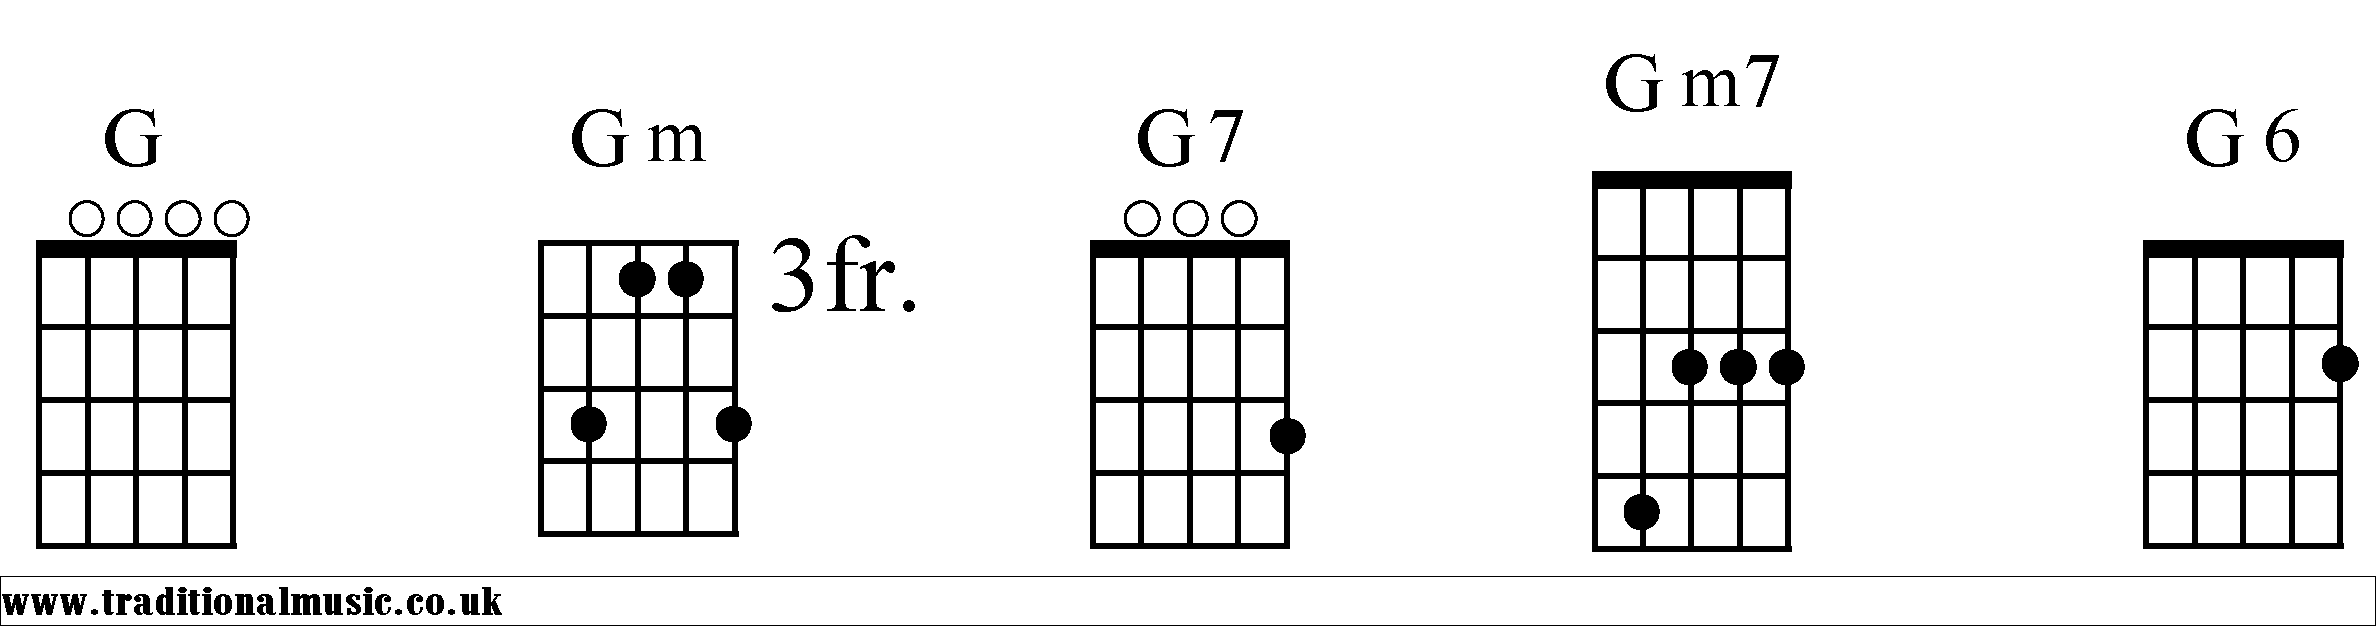
\includegraphics[scale=.15]{chords/Gbjo1}
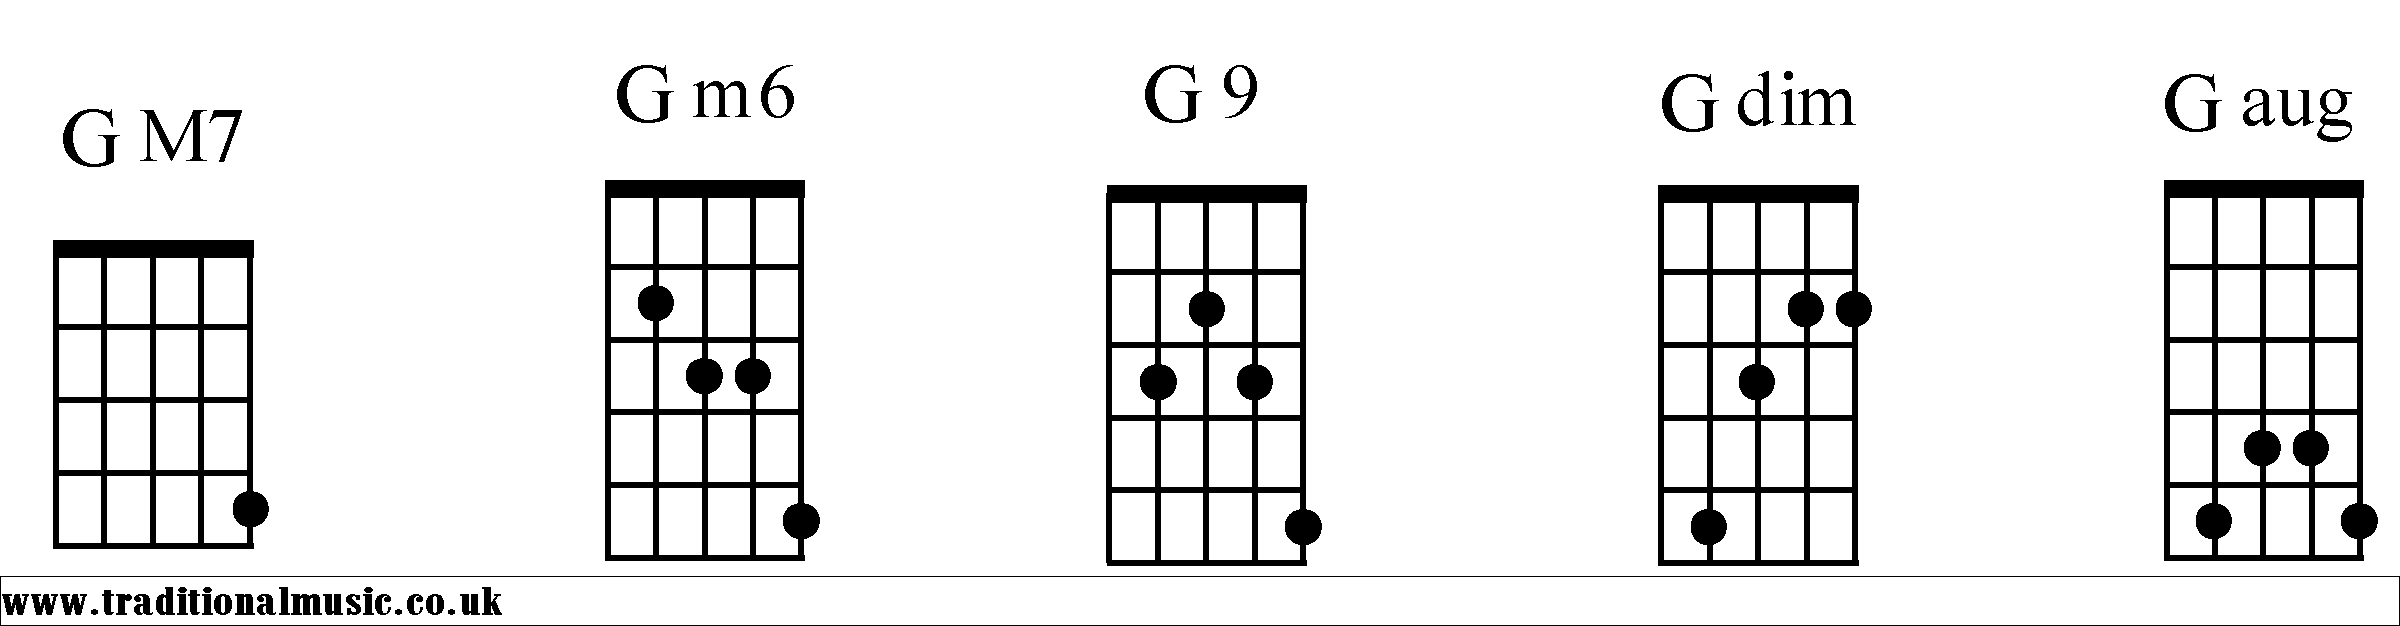
\includegraphics[scale=.15]{chords/Gbjo2}


\newpage
\chapter{Guitar Chords}


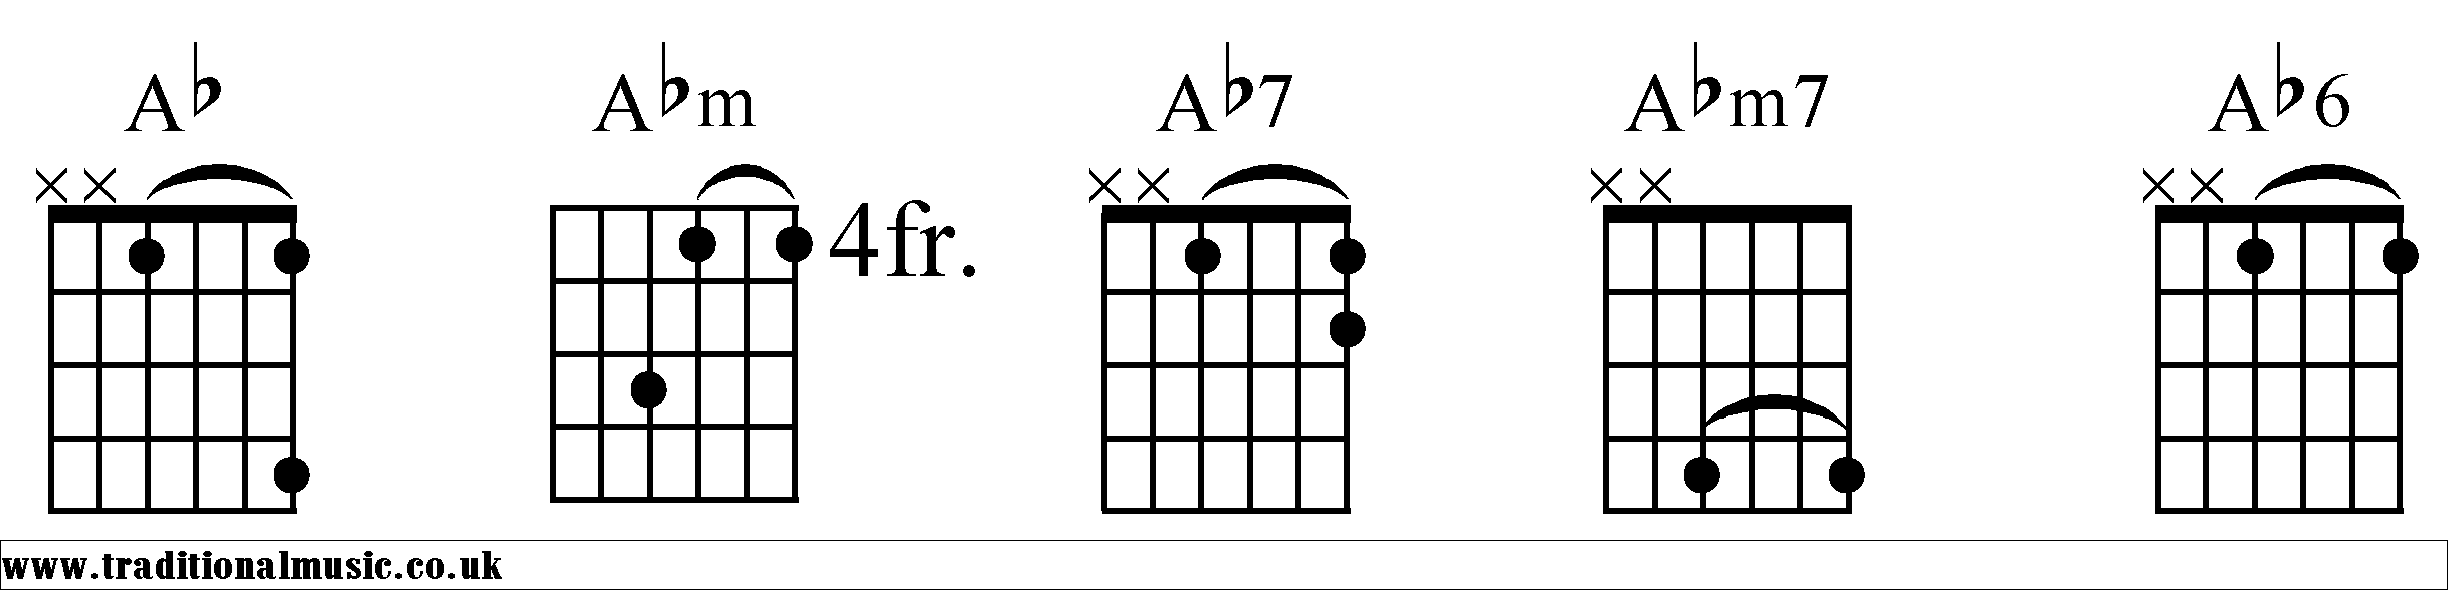
\includegraphics[scale=.15]{Abgtr1}
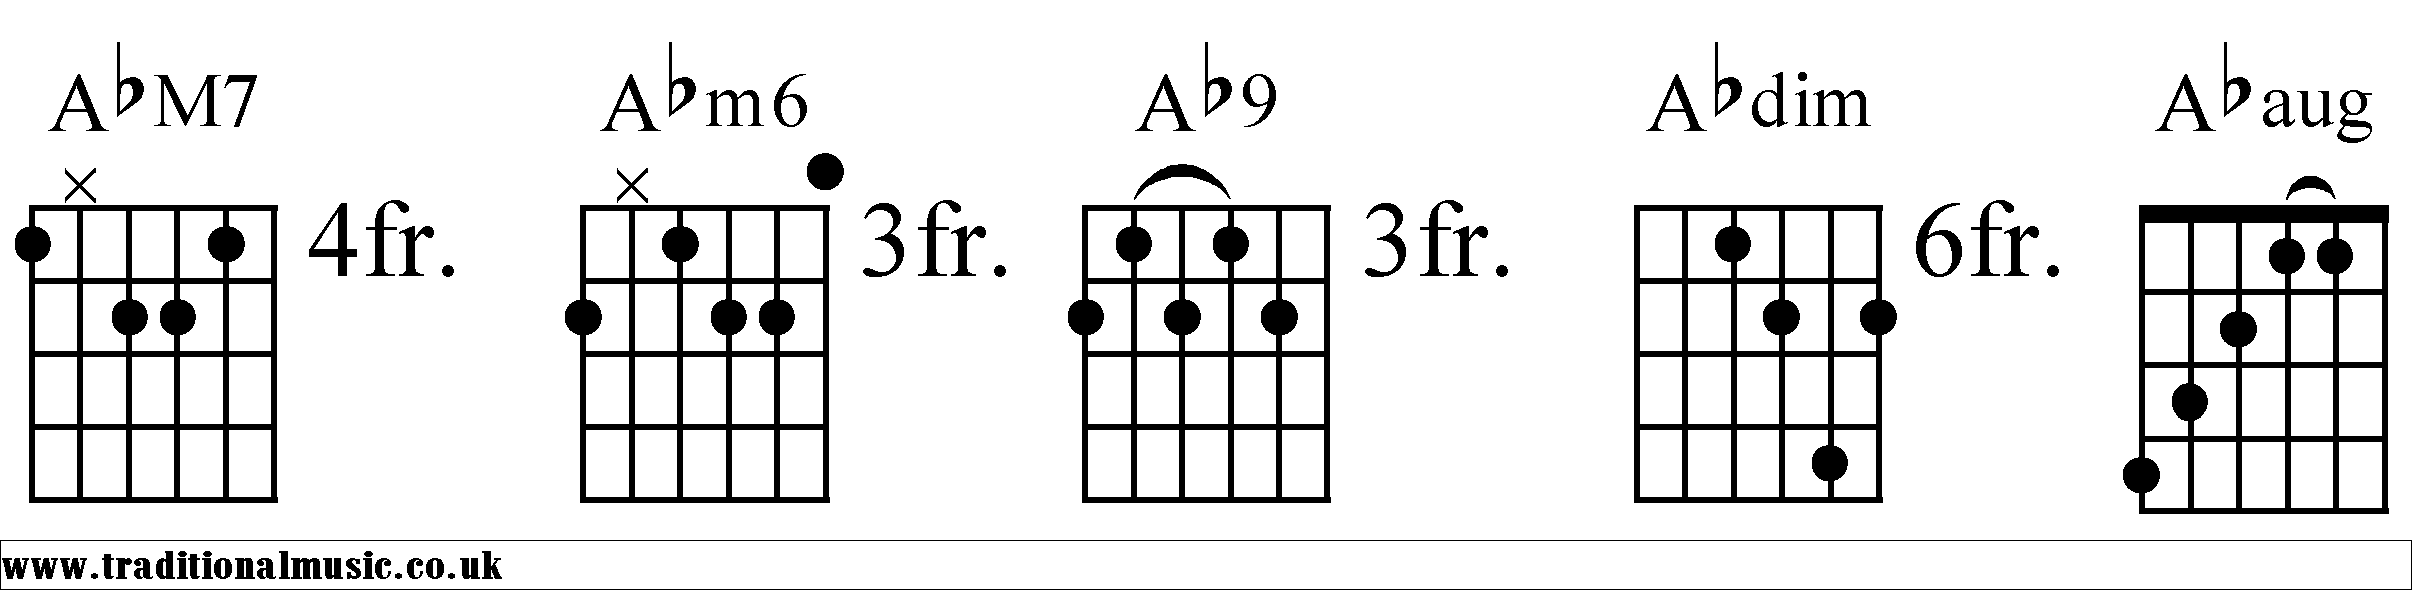
\includegraphics[scale=.15]{Abgtr2}

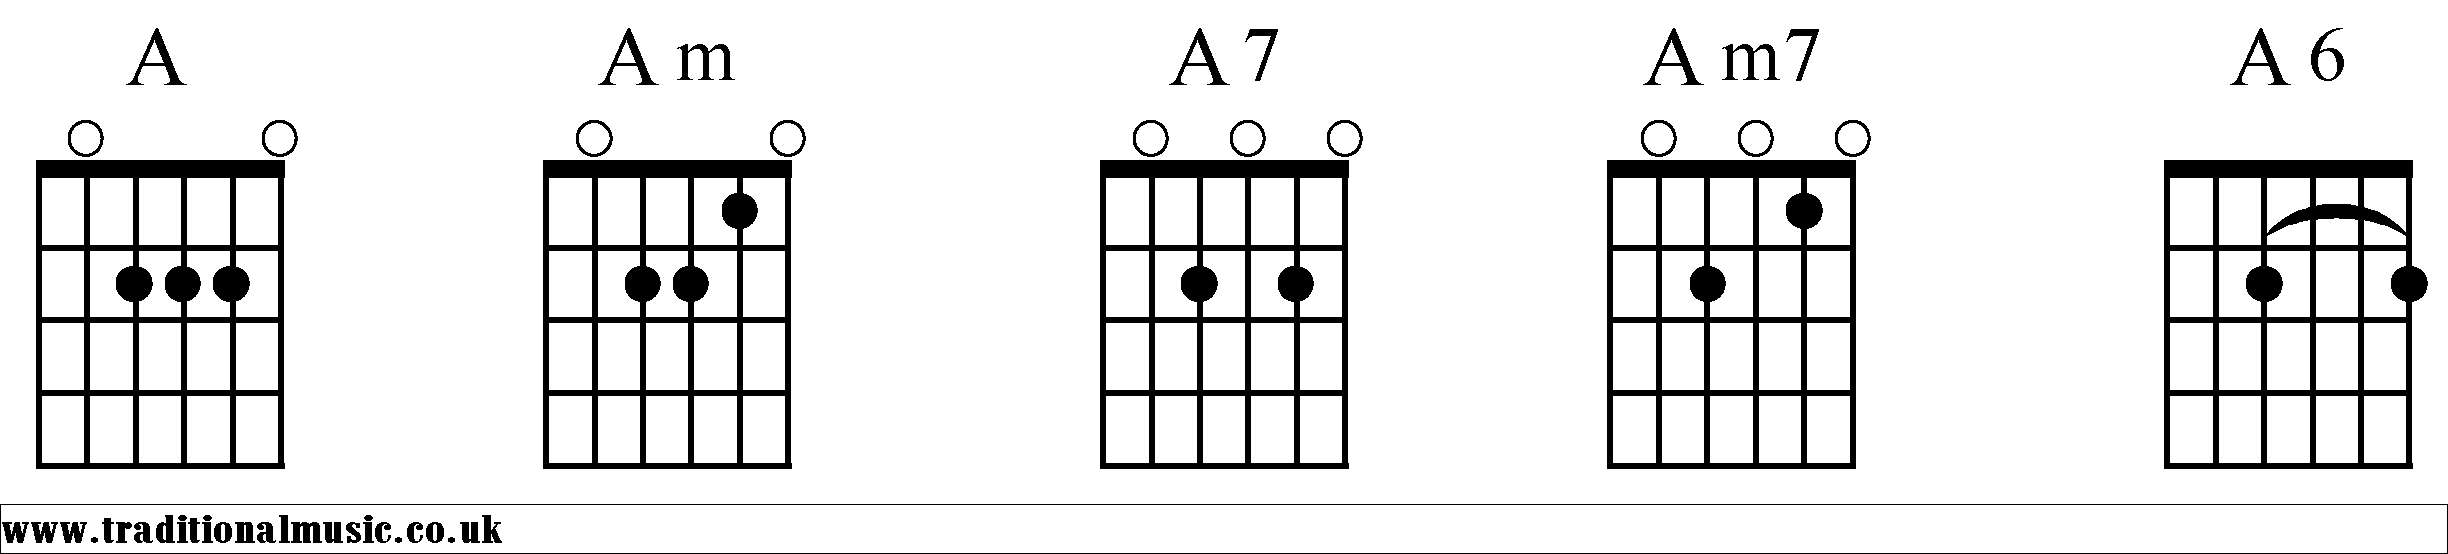
\includegraphics[scale=.15]{Agtr1}
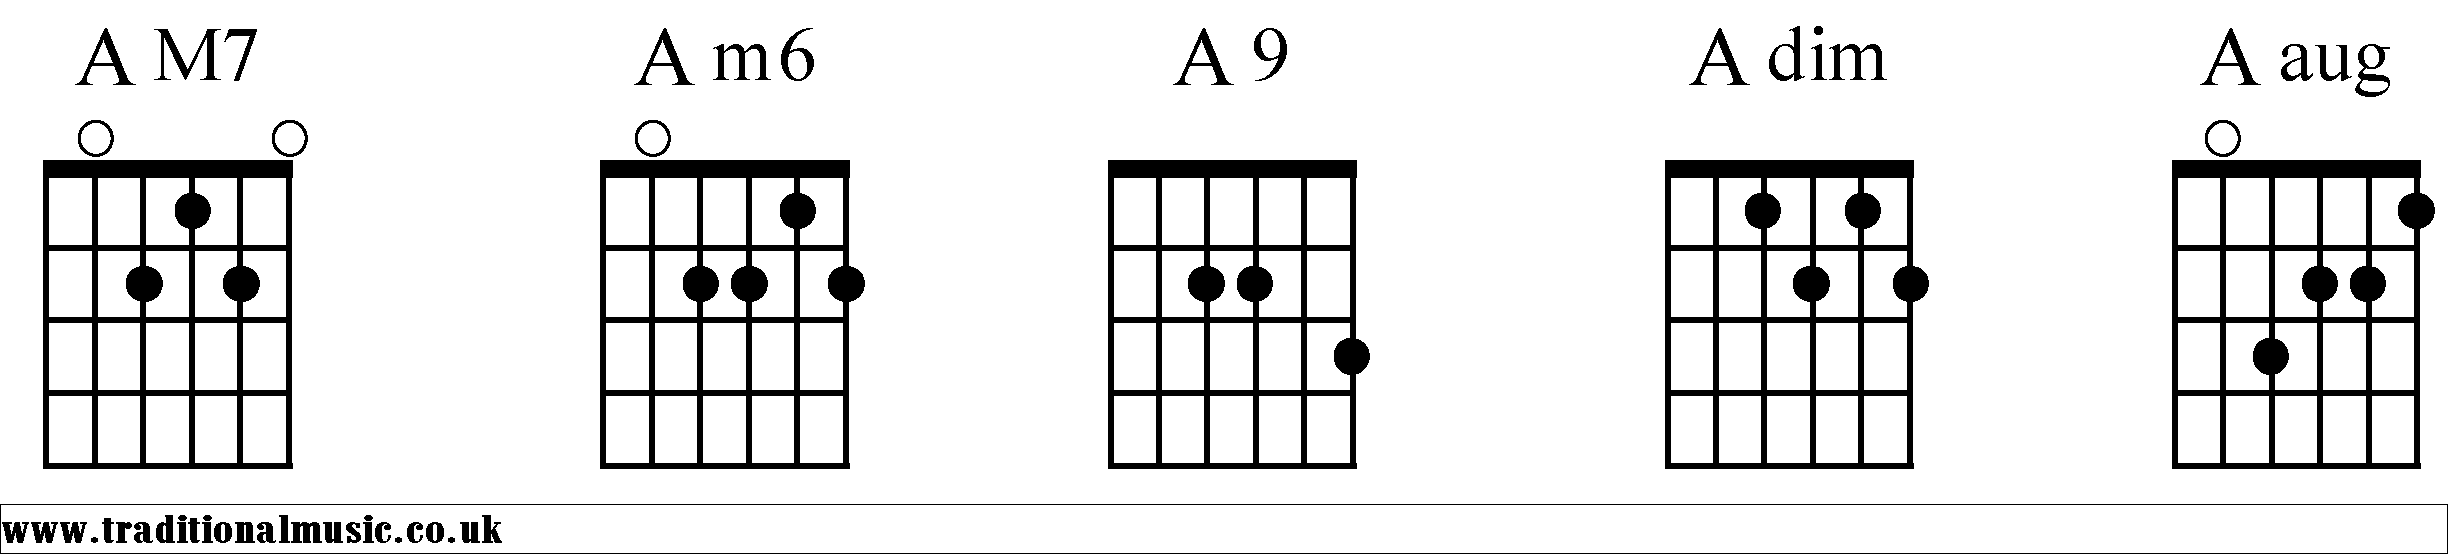
\includegraphics[scale=.15]{Agtr2}

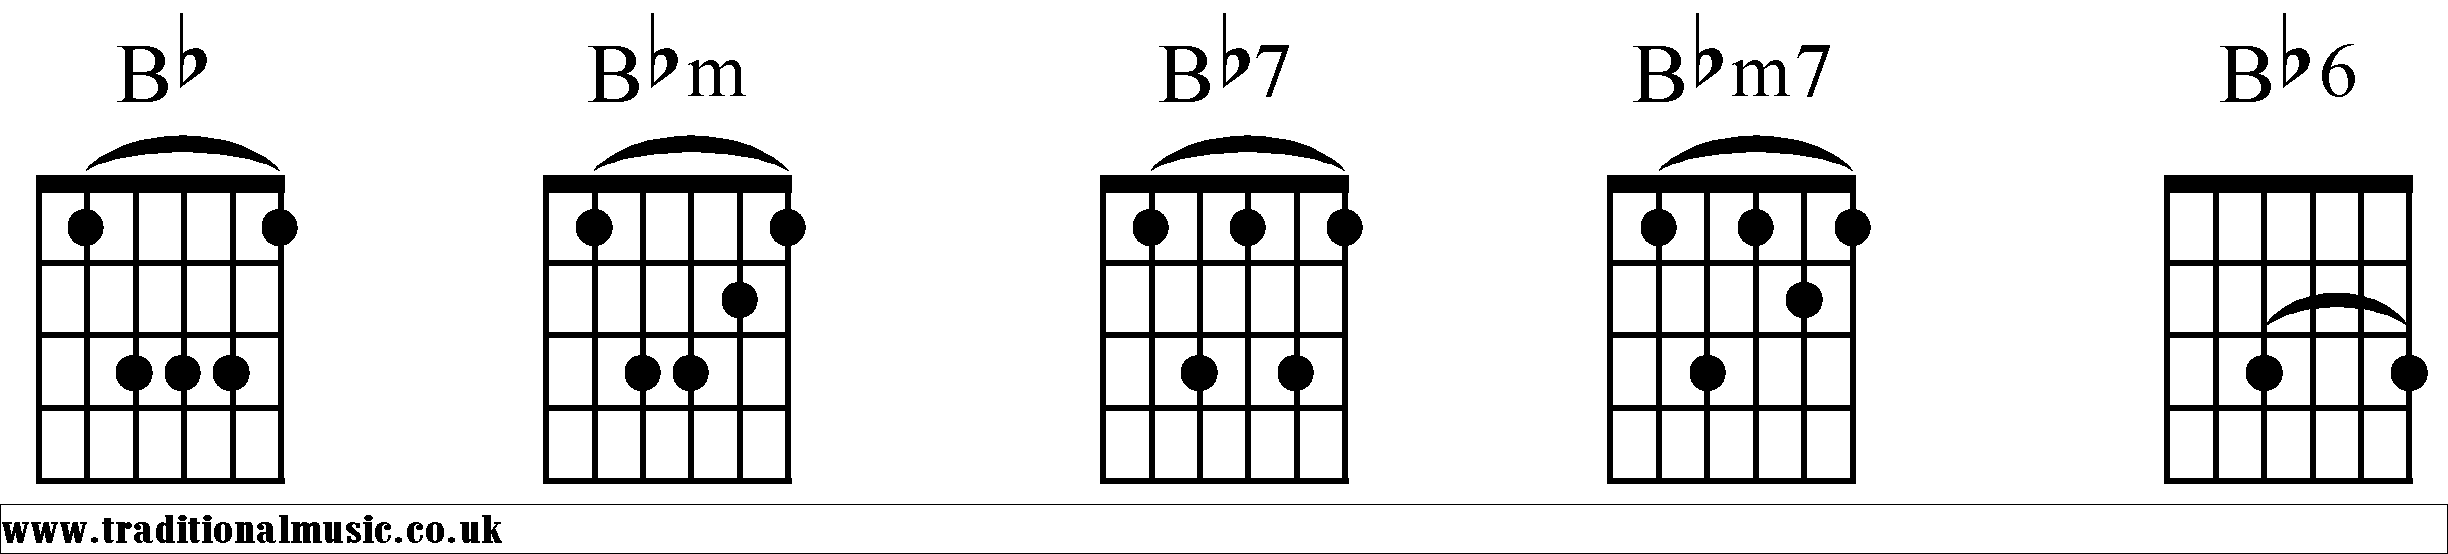
\includegraphics[scale=.15]{Bbgtr1}
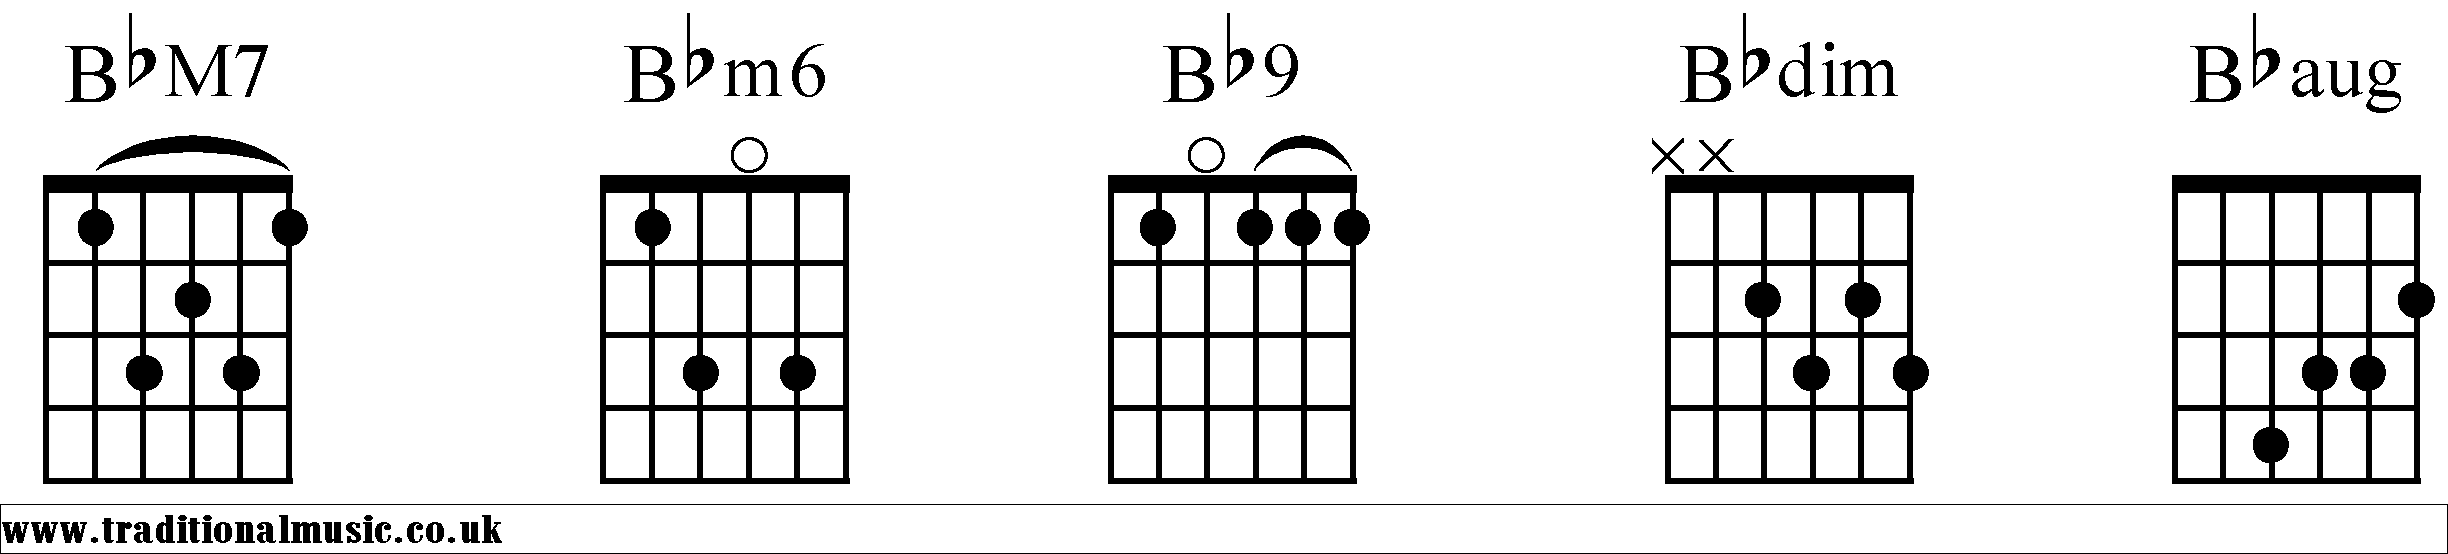
\includegraphics[scale=.15]{Bbgtr2}

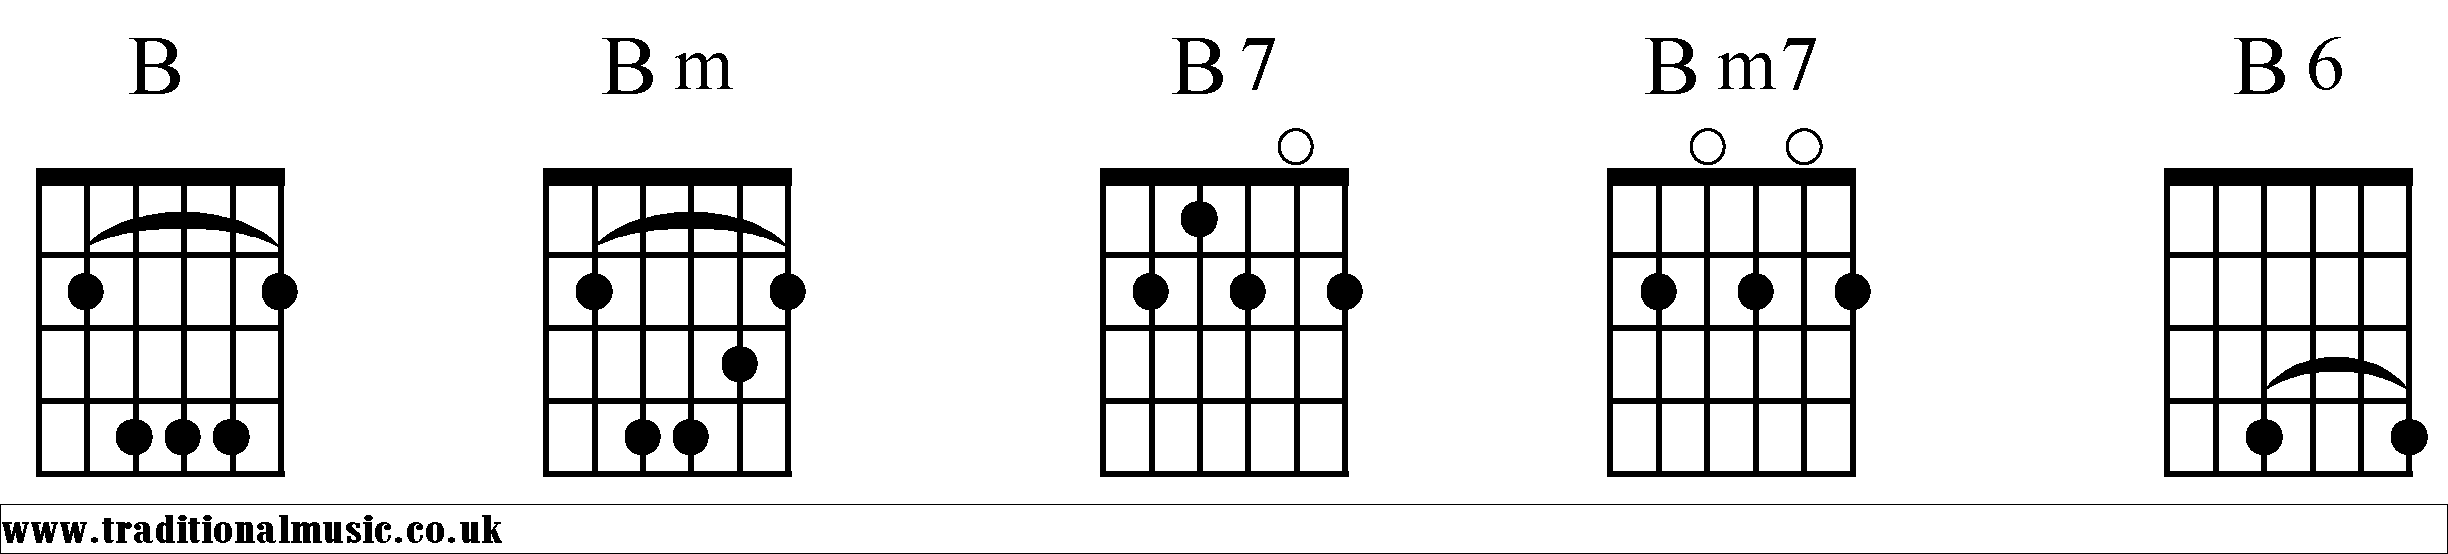
\includegraphics[scale=.15]{Bgtr1}
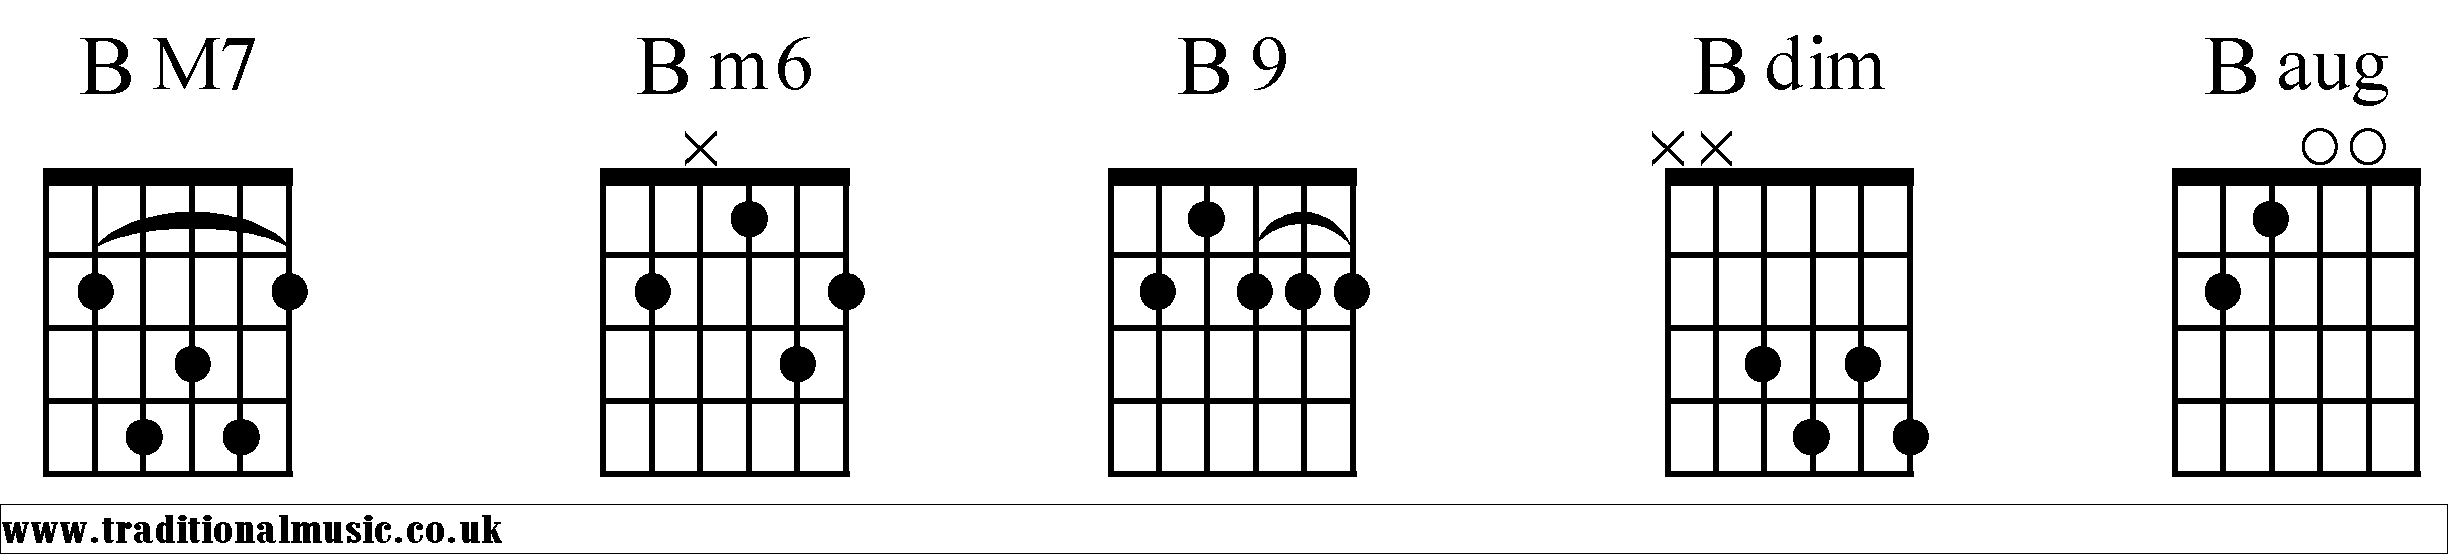
\includegraphics[scale=.15]{Bgtr2}

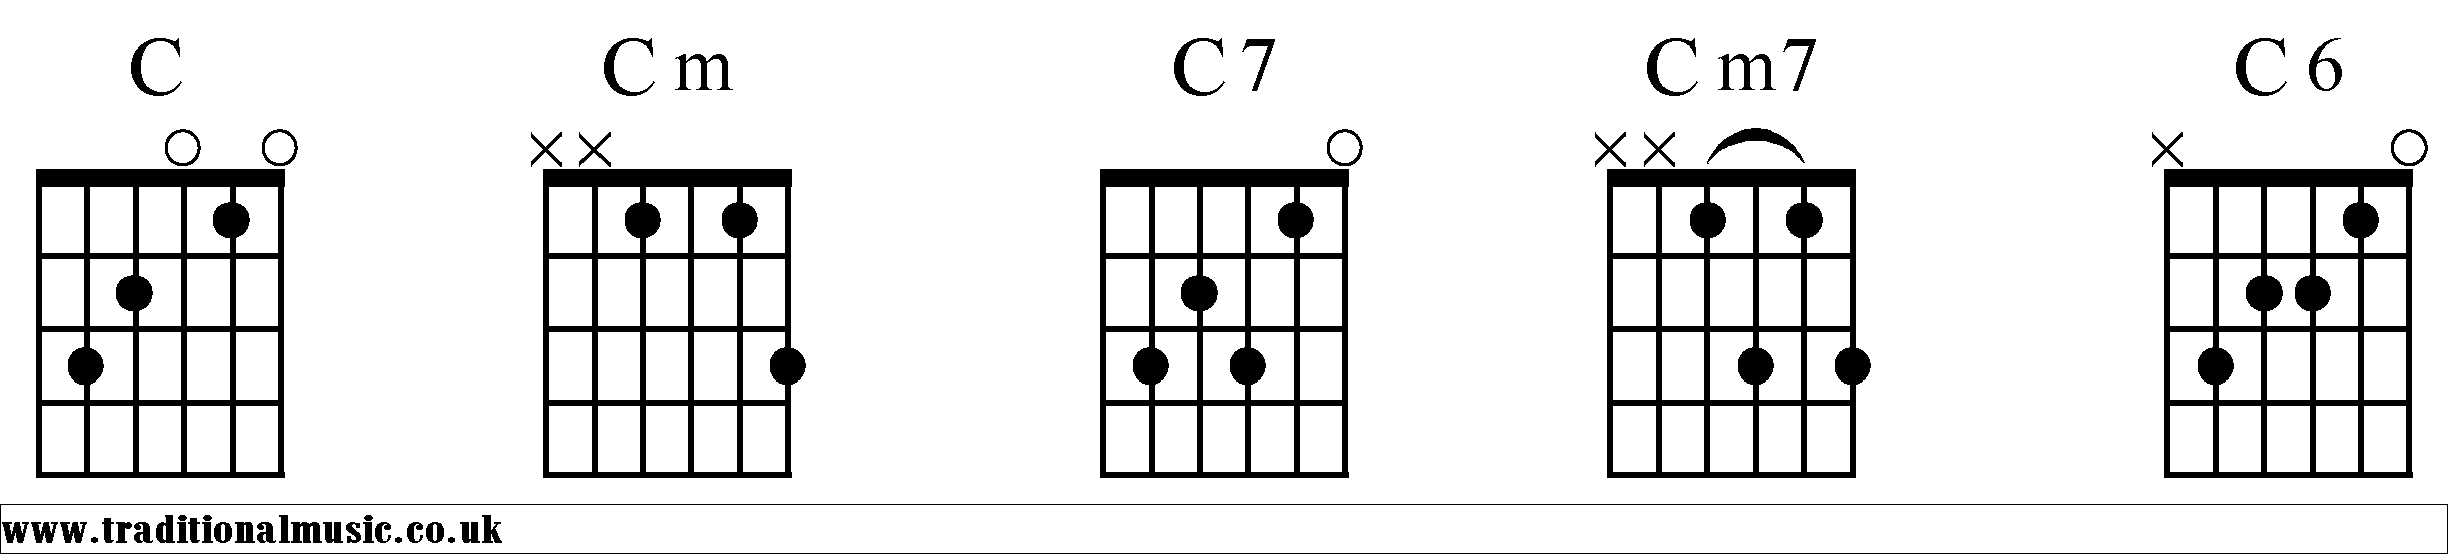
\includegraphics[scale=.15]{Cgtr1}
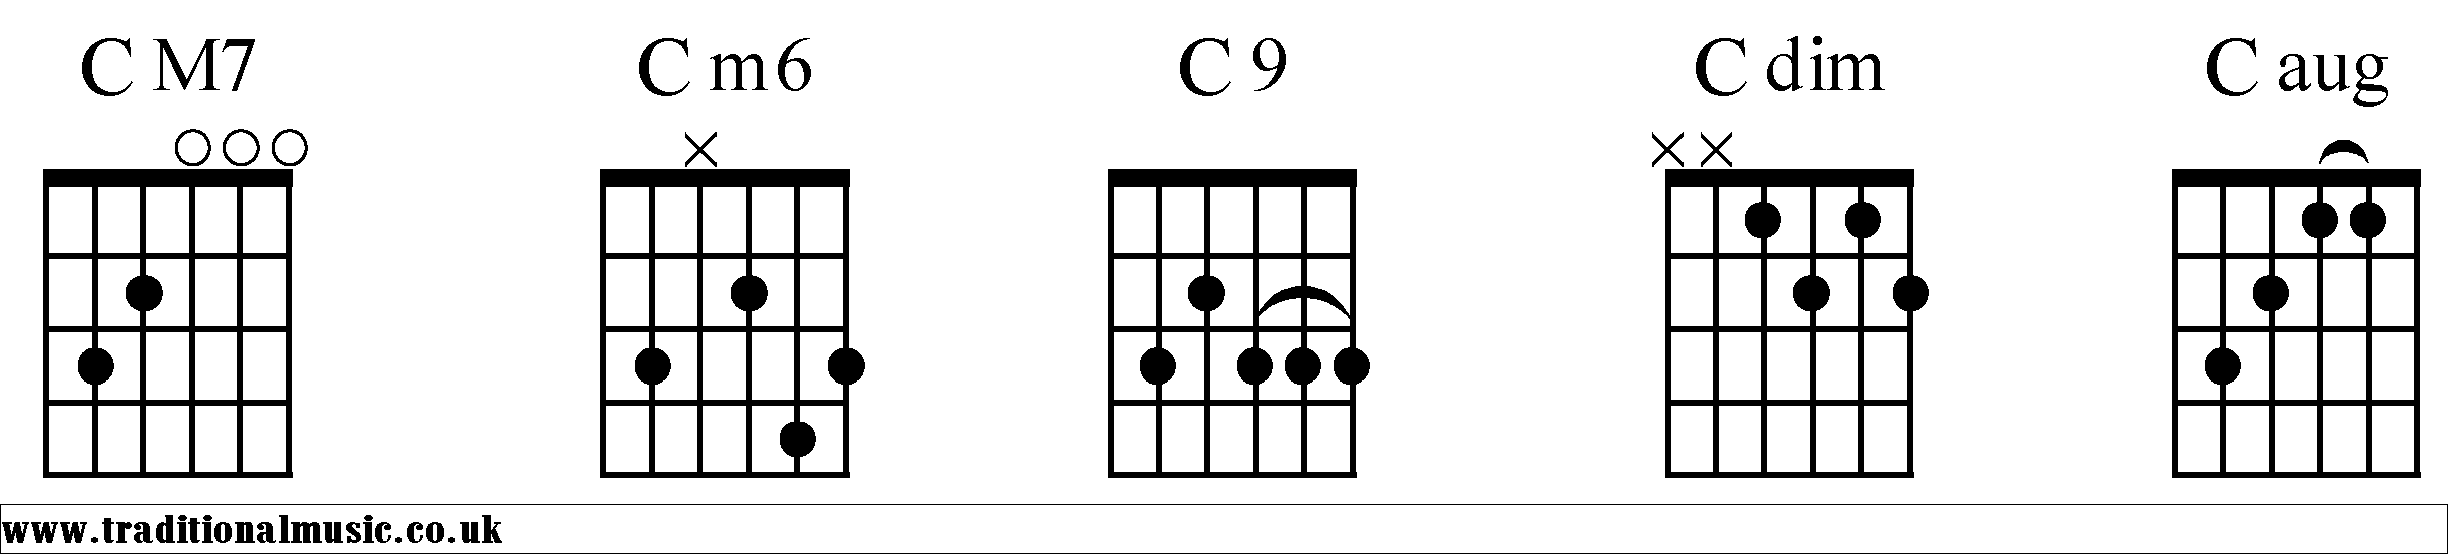
\includegraphics[scale=.15]{Cgtr2}

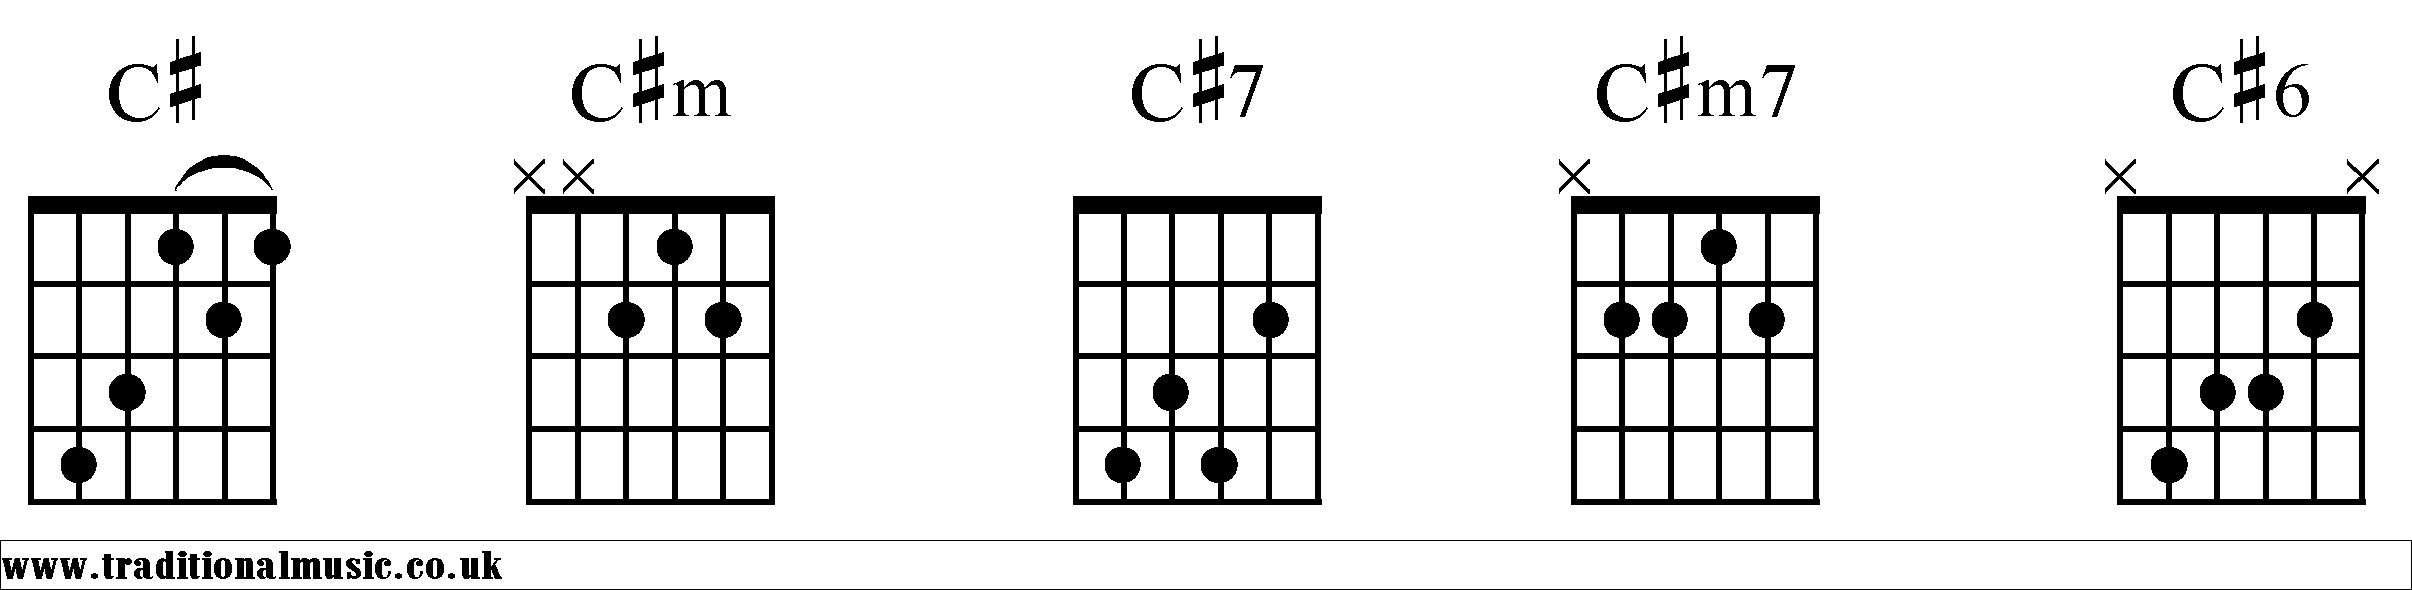
\includegraphics[scale=.15]{Csgtr1}
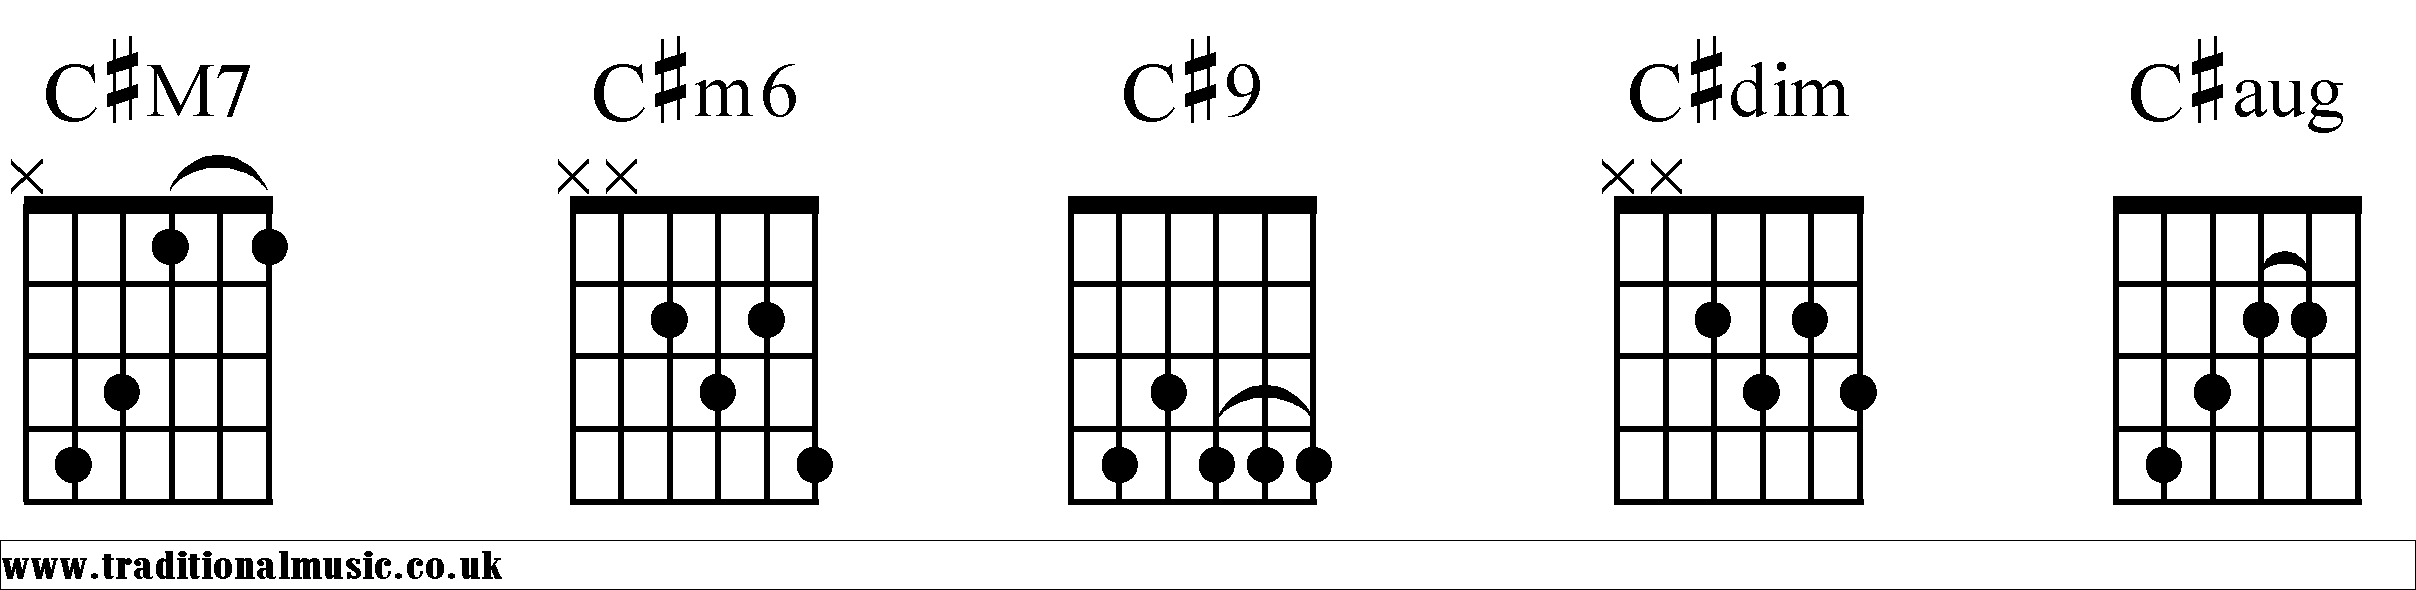
\includegraphics[scale=.15]{Csgtr2}

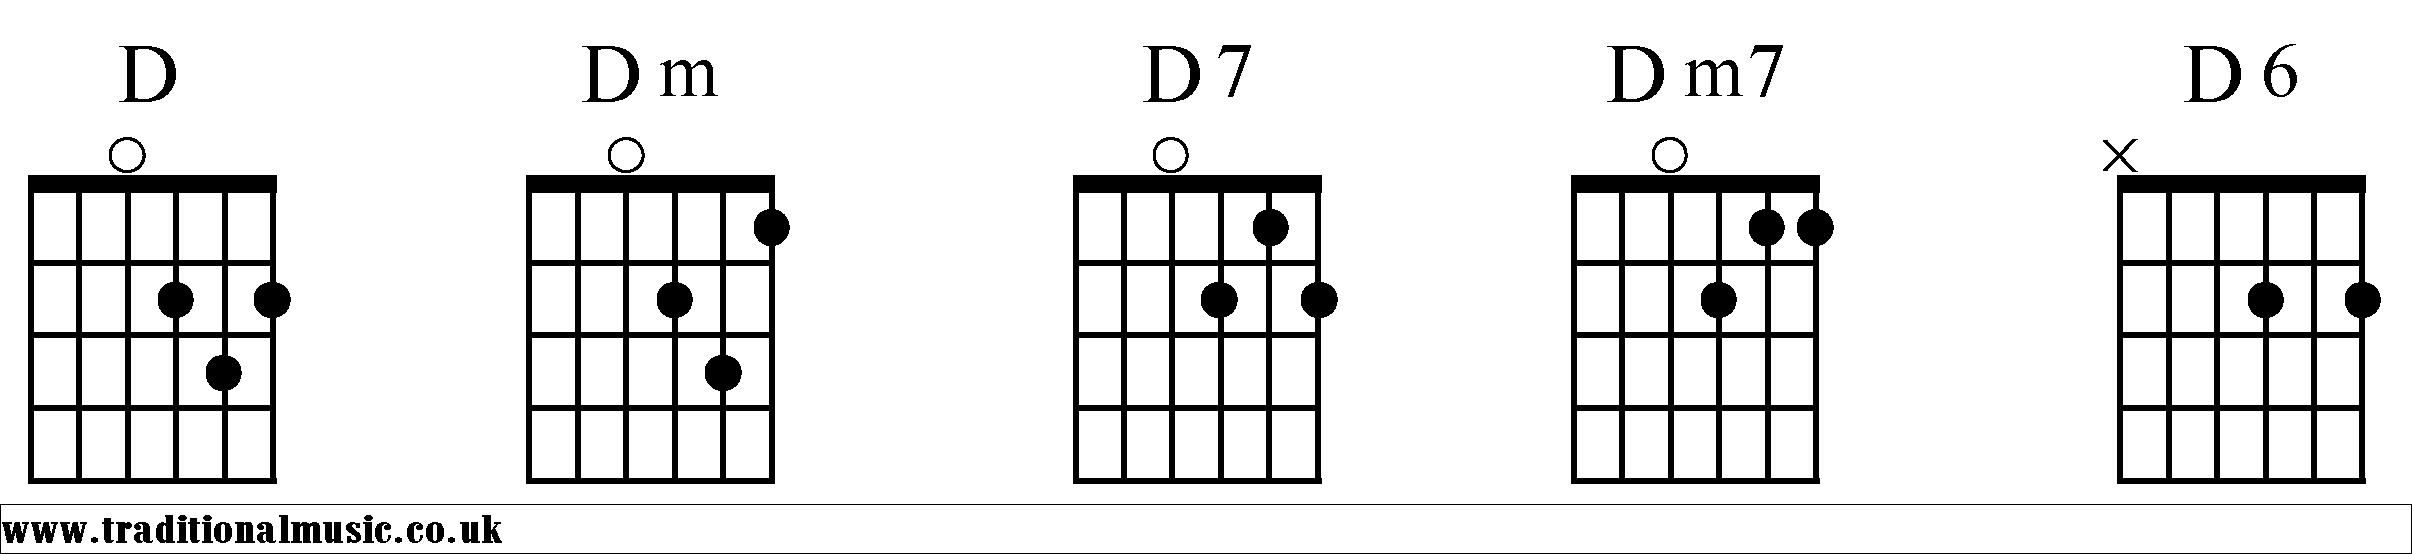
\includegraphics[scale=.15]{Dgtr1}
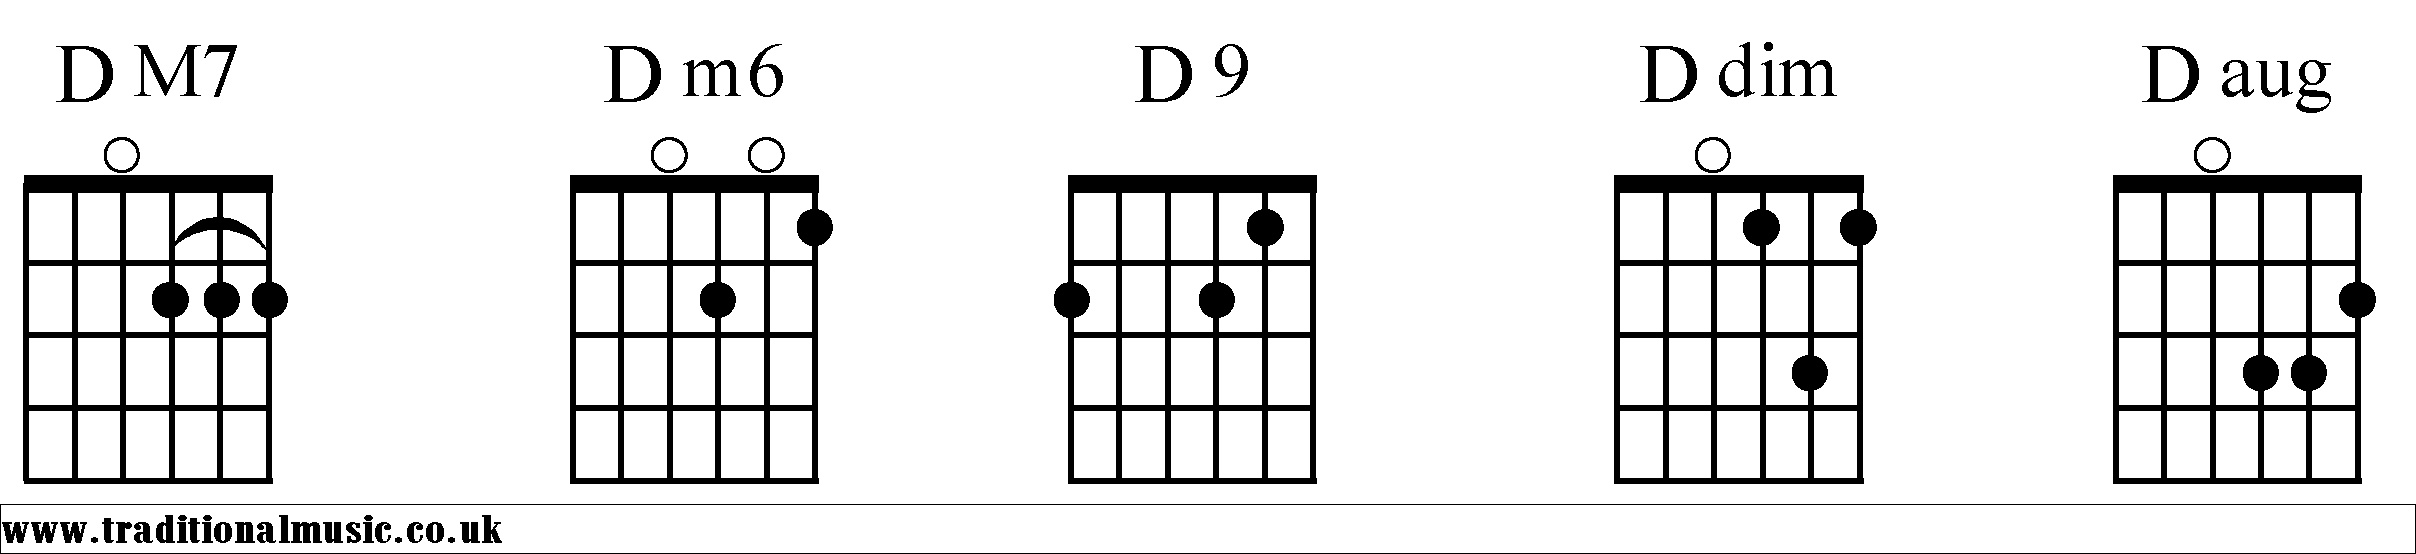
\includegraphics[scale=.15]{Dgtr2}

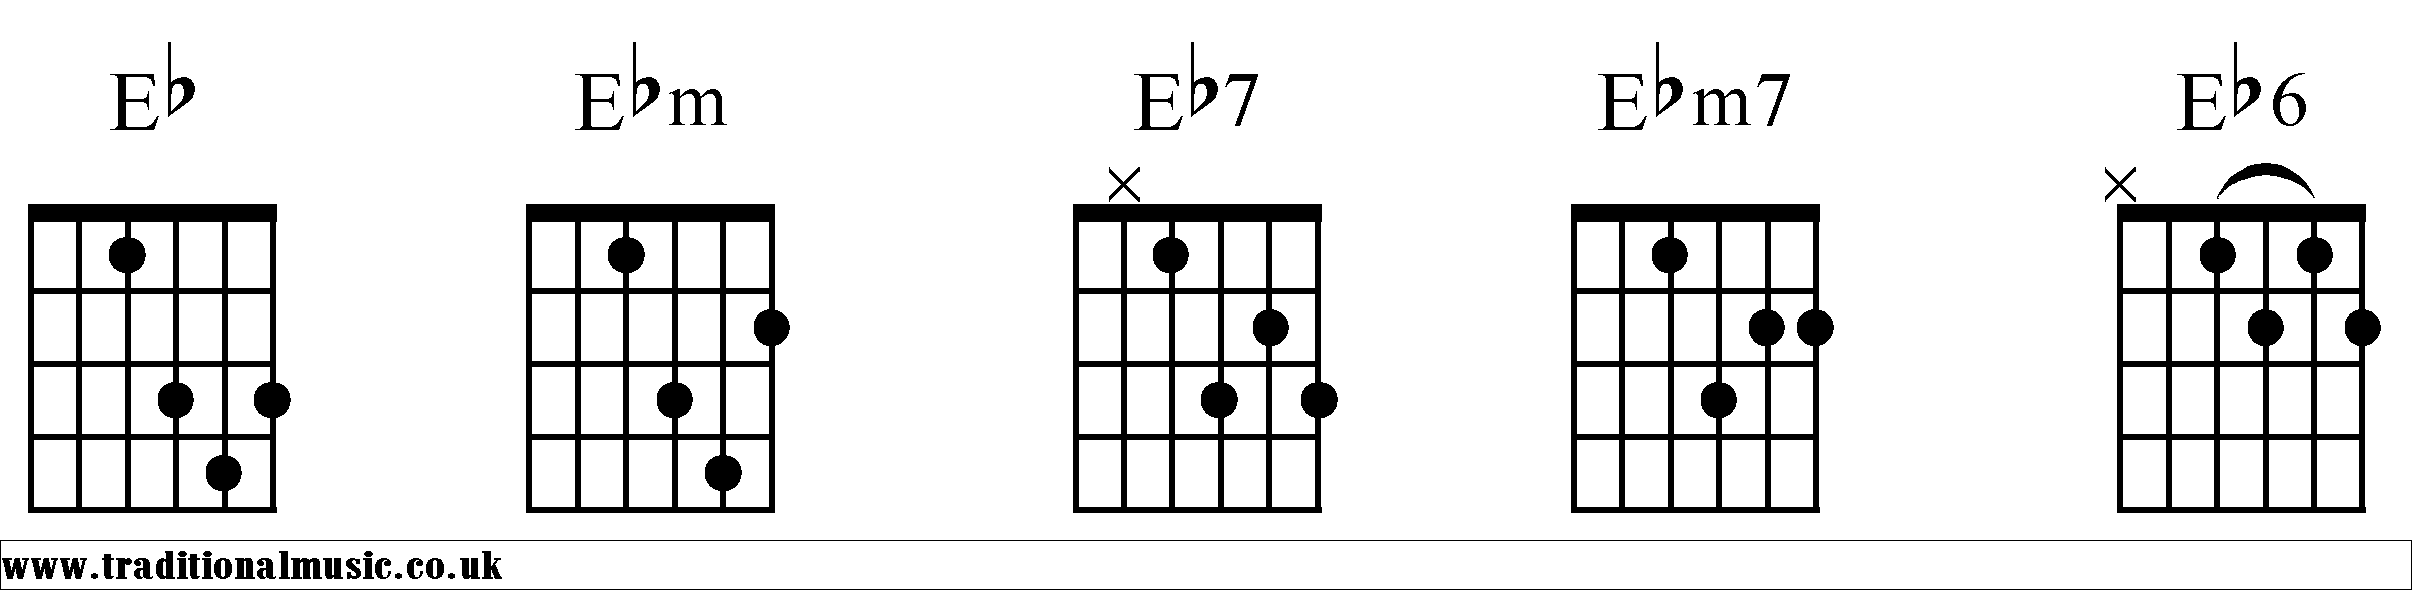
\includegraphics[scale=.15]{Ebgtr1}
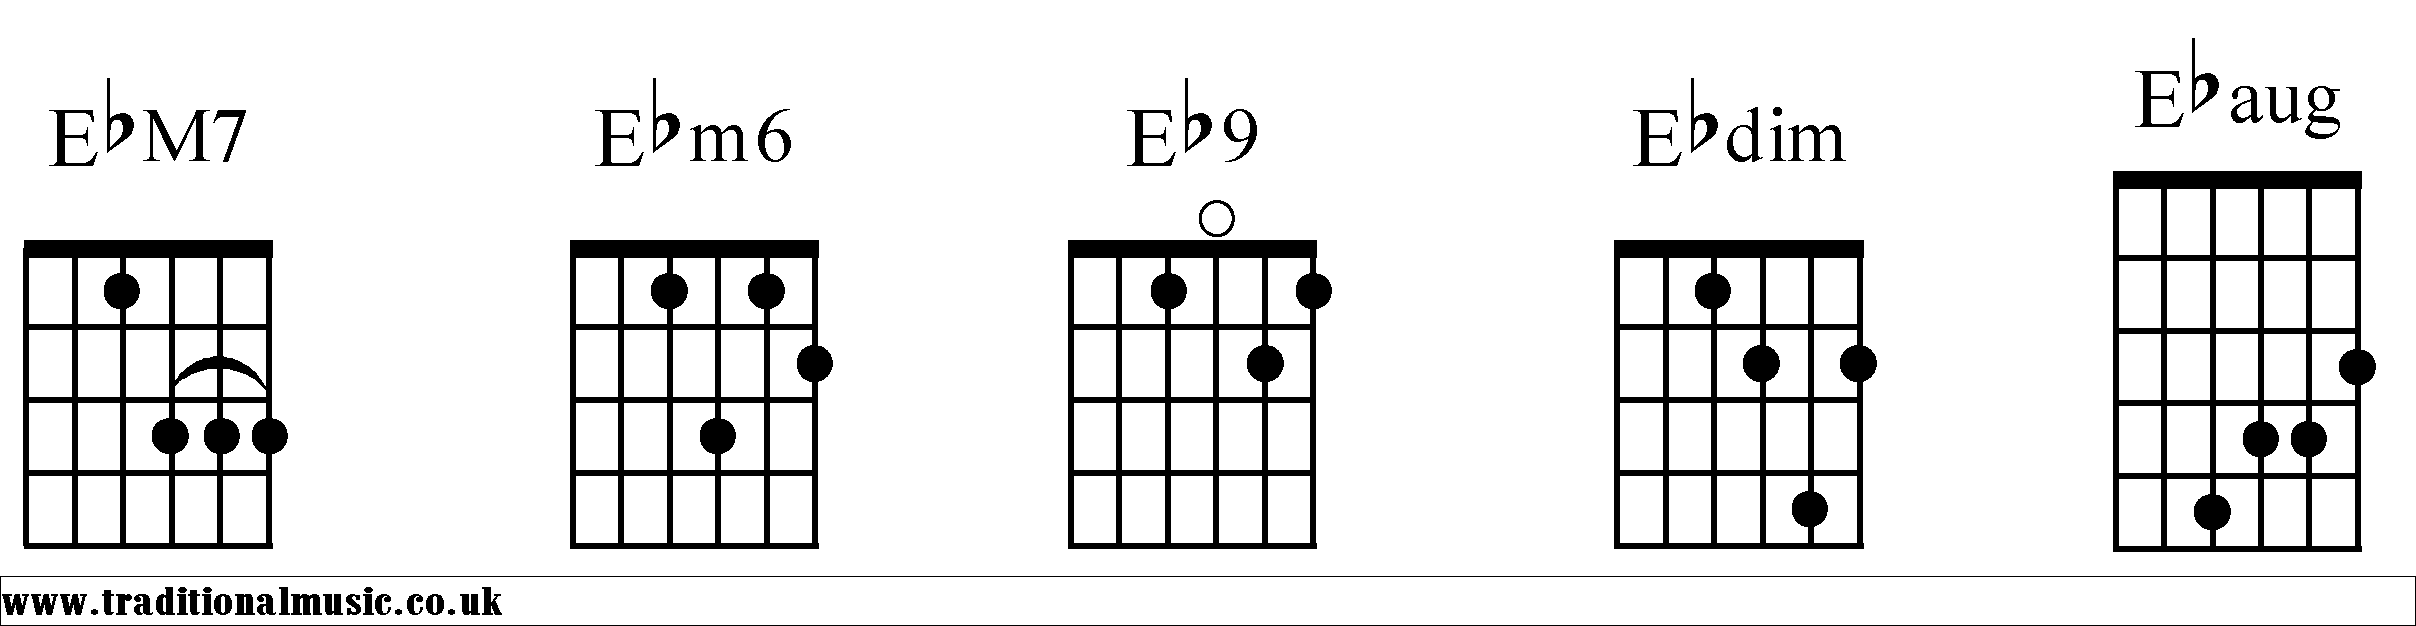
\includegraphics[scale=.15]{Ebgtr2}

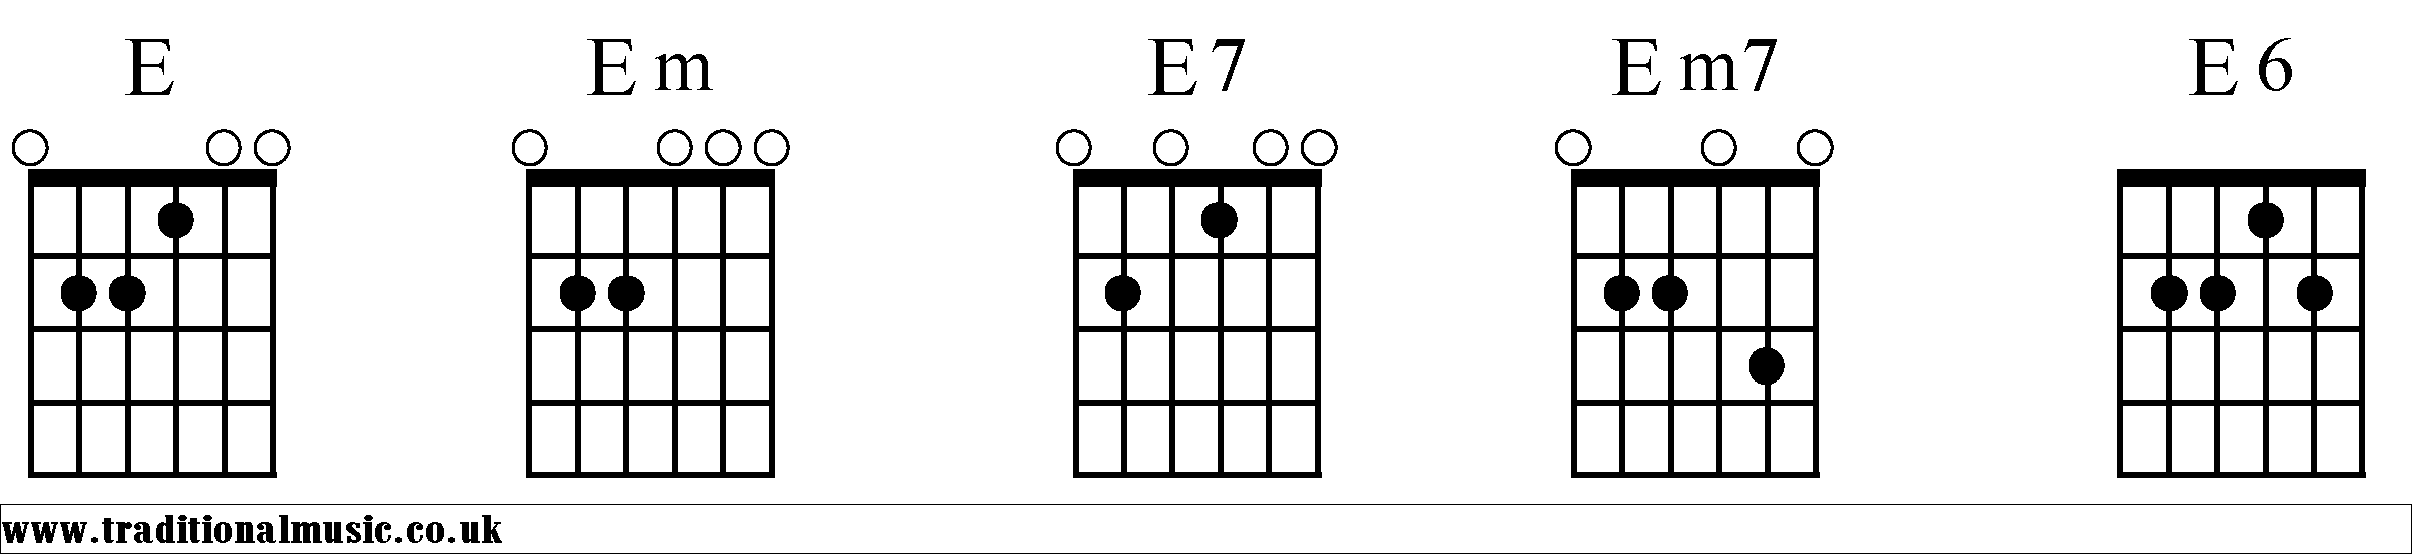
\includegraphics[scale=.15]{Egtr1}
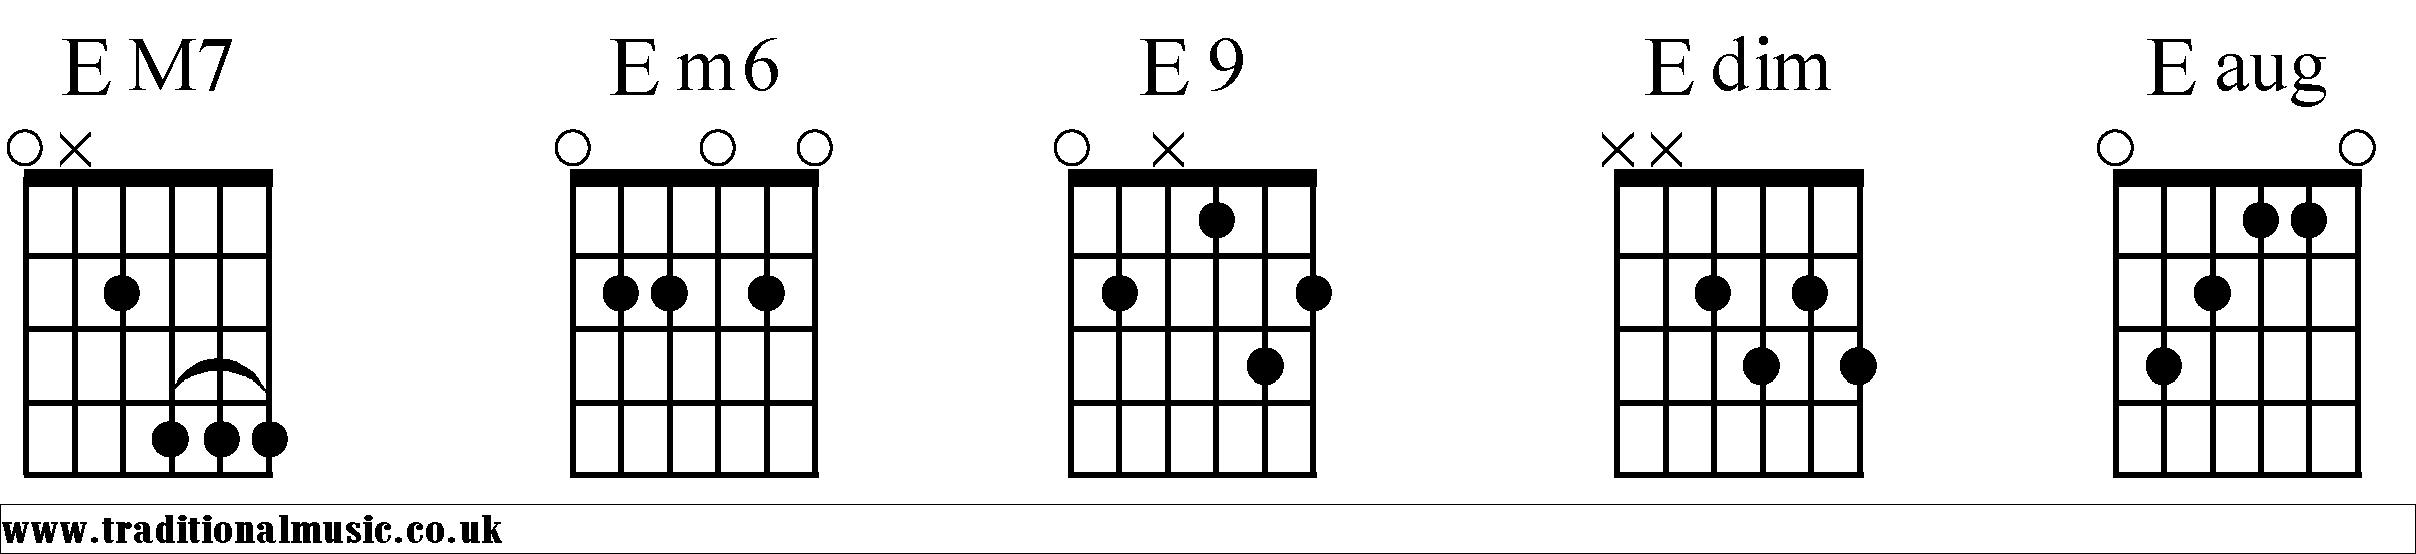
\includegraphics[scale=.15]{Egtr2}

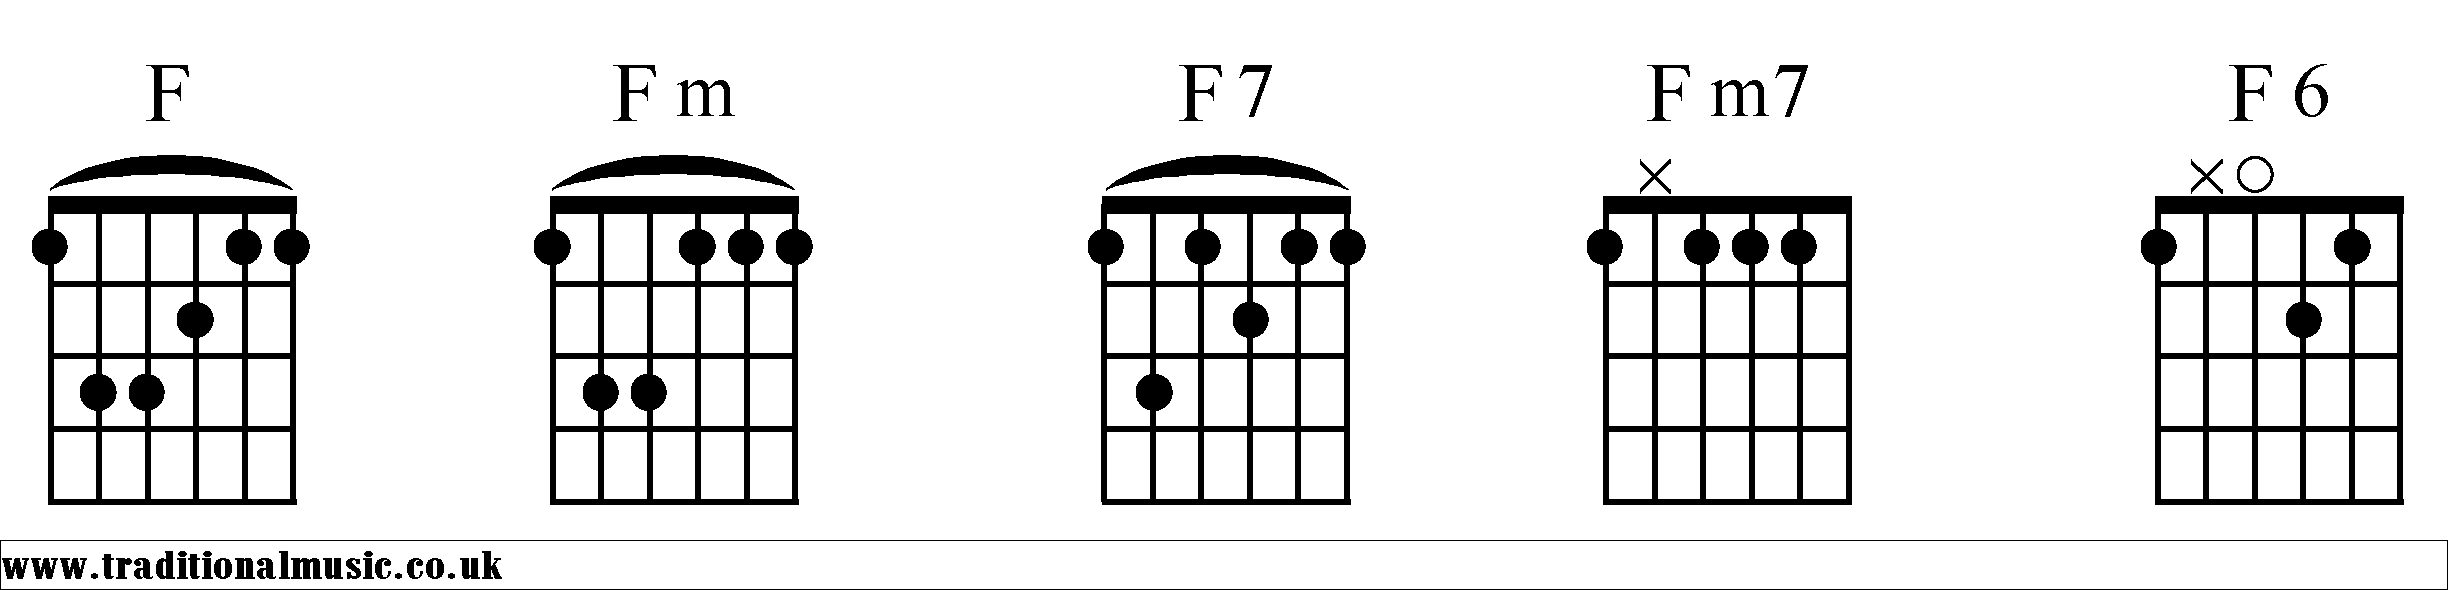
\includegraphics[scale=.15]{Fgtr1}
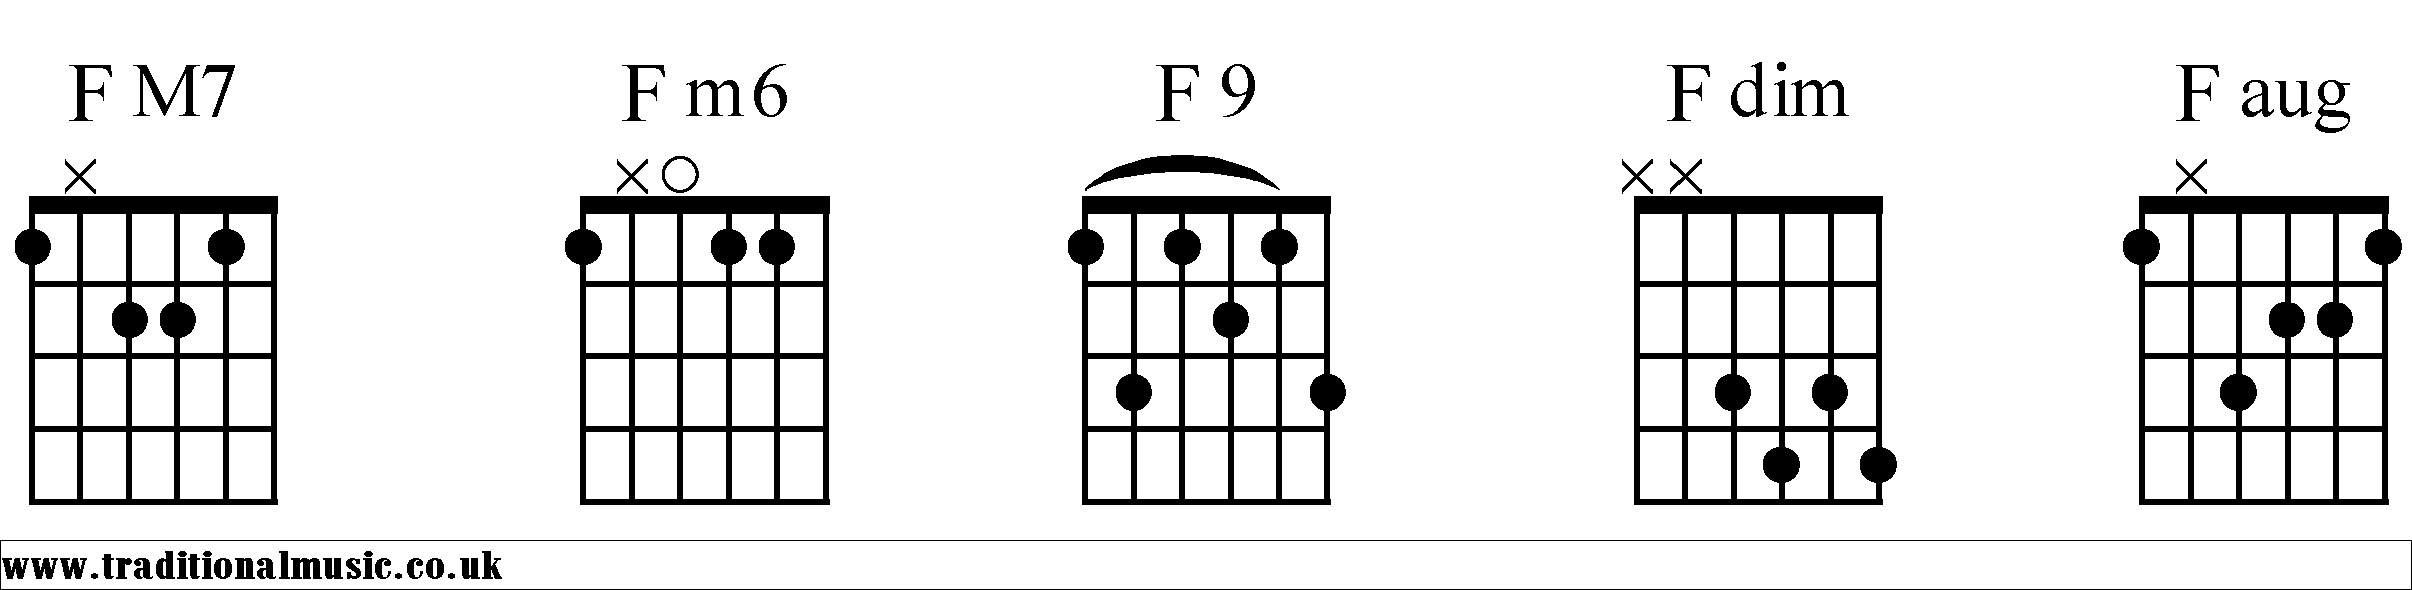
\includegraphics[scale=.15]{Fgtr2}

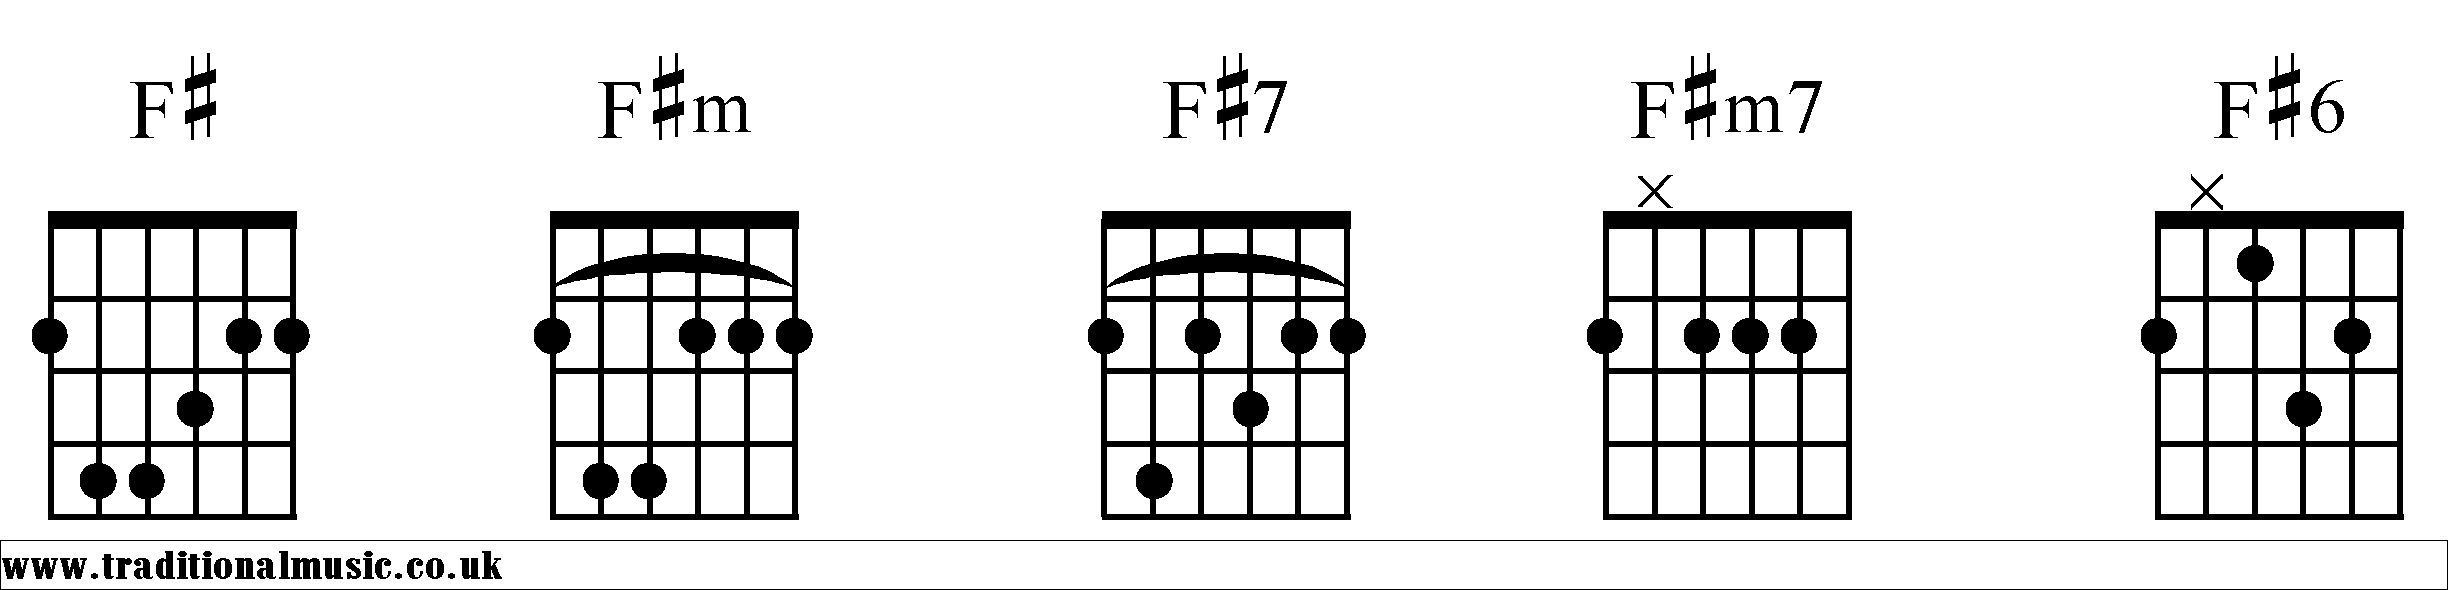
\includegraphics[scale=.15]{Fsgtr1}
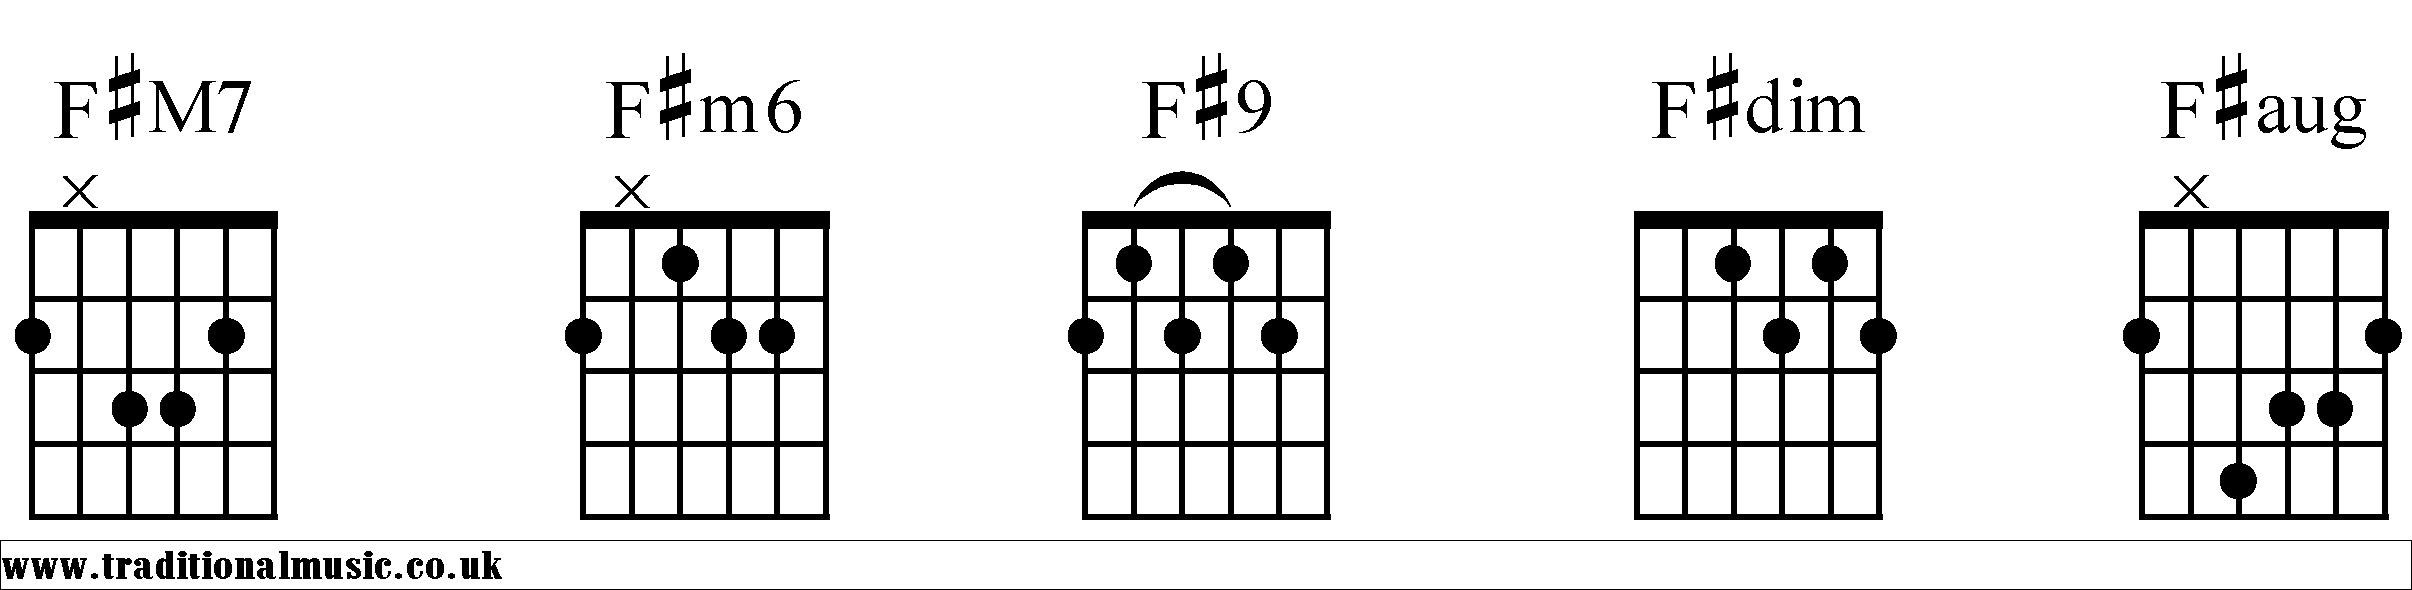
\includegraphics[scale=.15]{Fsgtr2}

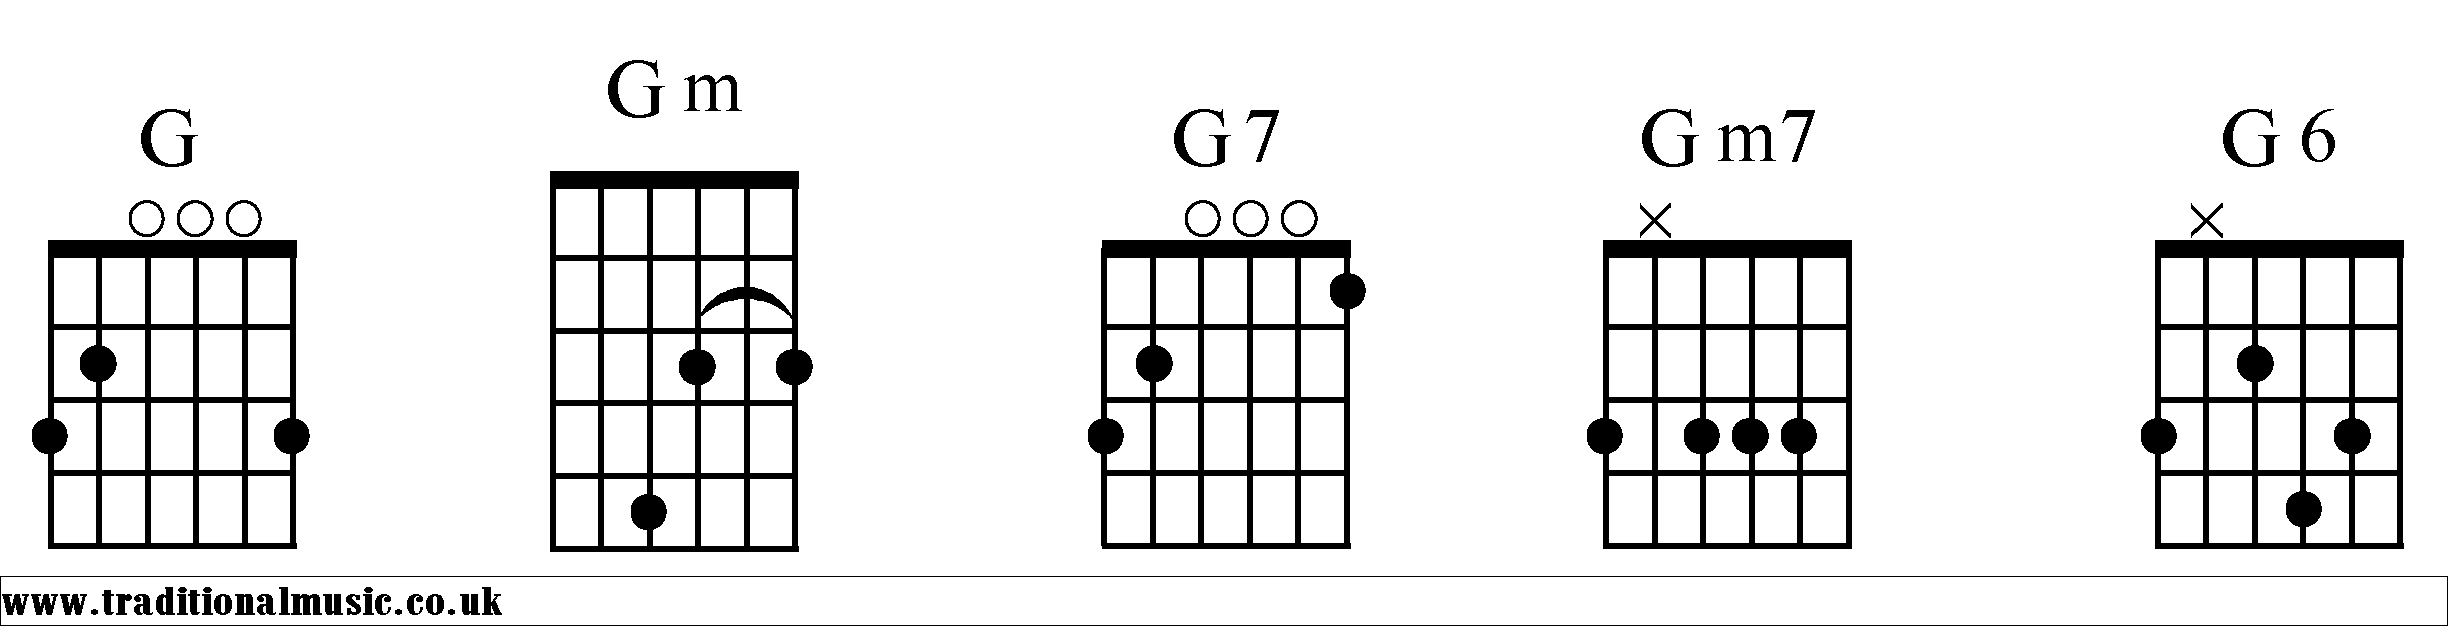
\includegraphics[scale=.15]{Ggtr1}
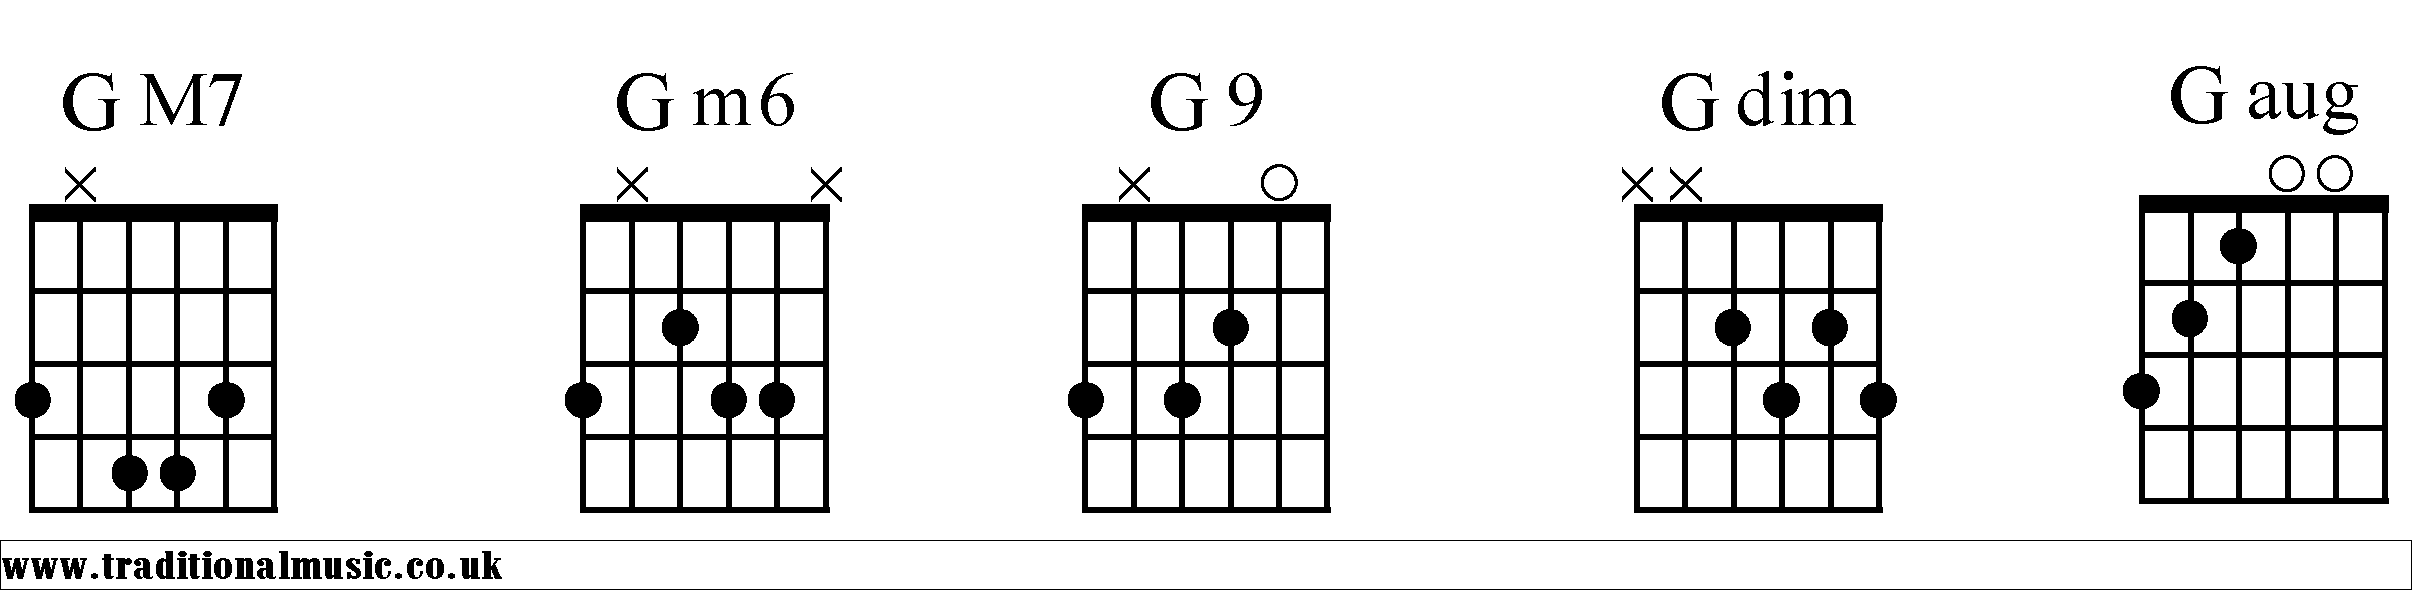
\includegraphics[scale=.15]{Ggtr2}


\end{document}
